\documentclass[12pt,a4paper,oneside]{report}

\usepackage[headheight=15pt, headsep=16pt, top=18mm, bottom=18mm, hmargin=22mm]{geometry}
\usepackage[T1]{fontenc}
\usepackage[utf8]{inputenc}
\usepackage{lmodern}
\usepackage{graphicx}
\usepackage{tikz}
\usepackage{parskip}
\usepackage{setspace}
\usepackage{refcount}
\usepackage{amsmath, amssymb}
\usepackage{amsthm}
\usepackage{adjustbox}
\usepackage{booktabs}
\usepackage{array}
\usepackage{tabularx}
\usepackage{longtable}
\usepackage{multirow}
\usepackage{makecell}
\usepackage{dirtree}
\usepackage{float}
\usepackage{placeins}
\usepackage{enumitem}
\usepackage[table]{xcolor}
\usepackage{csquotes}
\usepackage{fancyhdr}
\usepackage{titlesec}
\usepackage{subcaption}
\usepackage[most]{tcolorbox}
\tcbuselibrary{minted}
% tcolorbox writes temporary listing files into the LaTeX output directory;
% minted v3 no longer exposes an outputdir package option. The source defaults
% to the VS Code output directory (`out`); the Makefile overrides this through
% a generated wrapper so its `out_submit` build remains isolated.
\providecommand{\fedctlbuildoutputdir}{out}
\makeatletter
\edef\minted@outputdir{\fedctlbuildoutputdir/}
\makeatother
\usepackage{algorithm}
\usepackage{algpseudocode}
\usepackage{xurl}
\usepackage{hyperref}
\usepackage[backend=biber,style=authoryear-comp,maxcitenames=2,uniquelist=false,sorting=nyt]{biblatex}
\setcounter{biburllcpenalty}{100}
\setcounter{biburlucpenalty}{200}
\setcounter{biburlnumpenalty}{100}
\addbibresource{references.bib}
\usetikzlibrary{arrows.meta,calc,positioning}

\definecolor{paletteGreen}{HTML}{2A6F62}
\definecolor{paletteOrange}{HTML}{D96C3D}
\definecolor{coreblue}{RGB}{230,240,255}
\definecolor{darkblue}{RGB}{30,60,120}
\definecolor{fedavggreen}{HTML}{2A6F62}
\definecolor{heteroflblue}{HTML}{2E5FA7}
\definecolor{fedrolexpurple}{HTML}{7A4BA3}
\definecolor{fiarsered}{HTML}{B54747}
\definecolor{fedbuffteal}{HTML}{1D7A73}
\definecolor{fedstalebrown}{HTML}{8A5A2B}
\definecolor{codeFrame}{HTML}{E4E4E4}
\colorlet{evalBestText}{fiarsered}
\colorlet{evalSecondText}{heteroflblue}
\colorlet{codeBadgeBack}{paletteGreen!12!white}
\colorlet{codeBadgeFrame}{paletteGreen!75!black}
\newcommand{\evalbest}[1]{\textcolor{evalBestText}{{\bfseries\boldmath #1}}}
\newcommand{\evalsecond}[1]{\textcolor{evalSecondText}{#1}}
\newcommand{\evalcensored}[1]{\(\ge #1\)\textsuperscript{\(\ddagger\)}}

\hypersetup{
  colorlinks=true,
  linkcolor=paletteGreen,
  citecolor=paletteGreen,
  urlcolor=paletteGreen,
  filecolor=paletteGreen
}

\pagestyle{fancy}
\fancyhf{}
\fancyhead[L]{\nouppercase{\rightmark}}
\fancyhead[R]{\thepage}
\renewcommand{\headrulewidth}{0.4pt}

\newtcolorbox{aimbox}{
  colback=coreblue,
  colframe=white,
  boxrule=0pt,
  sharp corners,
  breakable
}

\newtcolorbox{definition}[1][]{%
  colback=paletteGreen!15!white,
  colframe=white,
  boxrule=0pt,
  sharp corners,
  breakable,
  before=\par\medskip,
  after=\par\medskip,
  #1
}

\newtcolorbox{paperbox}[1][]{
  colback=gray!4,
  colframe=paletteGreen!65!black,
  boxrule=0.35pt,
  sharp corners,
  breakable,
  #1
}

\newtheorem{theorem}{Theorem}[chapter]
\newtheorem{lemma}[theorem]{Lemma}


\font\codeLineNumberFont="Menlo" at 9pt
\renewcommand{\theFancyVerbLine}{{\codeLineNumberFont\arabic{FancyVerbLine}}}

\newtcblisting{codeblock}[2][]{
  breakable,
  enhanced,
  listing only,
  minted options app={
    mathescape,
    linenos,
    fontsize=\small,
    numbersep=10pt,
    xleftmargin=0.8em
  },
  minted language=#2,
  colback=gray!5,
  colframe=codeFrame,
  top=1pt,
  bottom=1pt,
  before skip=8pt,
  after skip=8pt,
  boxrule=0.2pt,
  overlay unbroken and first={
    \node[
      anchor=north east,
      fill=codeBadgeBack,
      draw=codeBadgeFrame,
      rounded corners=2pt,
      line width=0.45pt,
      inner xsep=5pt,
      inner ysep=2pt,
      font=\small\bfseries\ttfamily,
      text=codeBadgeFrame
    ] at ([xshift=-4pt,yshift=-3pt]interior.north east) {#2};
  },
  #1
}

\titleformat{\chapter}[hang]
  {\normalfont\bfseries}
  {\fontsize{60}{40}\selectfont\thechapter}
  {0.2em}
  {\fontsize{30}{30}\selectfont}

\titleformat{\section}
  {\normalfont\bfseries\Large}
  {\fontsize{19}{22}\selectfont\thesection}
  {0.6em}
  {}

\titleformat{\subsection}
  {\normalfont\bfseries\large}
  {\fontsize{16}{18}\selectfont\thesubsection}
  {0.6em}
  {}

\title{Fedctl: A Heterogeneous Testbed for Realistic Federated Learning}
\author{Haoran Jie}
\date{May 2026}
\newcommand{\declarationdate}{\number\day\space\ifcase\month\or January\or February\or March\or April\or May\or June\or July\or August\or September\or October\or November\or December\fi\space\number\year}
\newcommand{\candidatenumber}{3243Z}
\newcommand{\college}{Robinson College}
\newcommand{\coursethe}{Computer Science Tripos, Part III}
\newcommand{\coursefor}{Part III of the Computer Science Tripos}
\IfFileExists{\fedctlbuildoutputdir/generated-wordcount.tex}{%
  \input{\fedctlbuildoutputdir/generated-wordcount}%
}{%
  \newcommand{\mainwordcount}{UNKNOWN}%
  \newcommand{\mainwordcountplain}{UNKNOWN}%
}
\newcommand{\totalpagecount}{\ifsubmission 70\else 71\fi}
\newif\ifsubmission
% Uncomment for the anonymised submission copy:
% \submissiontrue

\begin{document}

\pagenumbering{gobble}
\begin{sffamily}
\begin{titlepage}
\makeatletter

\hspace*{-14mm}
\includegraphics[width=65mm]{figures/logo-dcst-colour}

\ifsubmission

\begin{center}
\Huge
\vspace{\fill}
\@title
\vspace{\fill}

\Large
Candidate \candidatenumber
\vspace{\fill}
\end{center}

\else

\begin{center}
\Huge
\vspace{\fill}
\@title
\vspace{\fill}

\@author
\vspace{10mm}

\Large
\college
\vfill

\@date
\vspace{\fill}
\end{center}

\fi

\vspace{\fill}
\begin{center}
Submitted in partial fulfilment of the requirements for the\\
\coursethe\\
University of Cambridge
\end{center}

\makeatother
\end{titlepage}

\clearpage
\makeatletter
\@tempcnta=\getpagerefnumber{lastcontentpage}\relax%
\advance\@tempcnta by -\getpagerefnumber{firstcontentpage}%
\advance\@tempcnta by 1%
\xdef\contentpages{\the\@tempcnta}%
\makeatother

Total page count: \totalpagecount

Main chapters (excluding front matter, bibliography and appendices):
\contentpages~pages
(pp~\pageref{firstcontentpage}--\pageref{lastcontentpage})

Main chapters word count: \mainwordcount

Methodology used to generate that word count:

\begin{quote}
\begin{verbatim}
$ texcount -merge -sum -q \
    1_introduction.tex 2_background.tex 3_related_work.tex \
    4_implementation.tex \
    5_evaluation.tex 6_conclusions.tex
\end{verbatim}
% \noindent Output used in this build: \texttt{\mainwordcountplain}
\end{quote}
\end{sffamily}

\vspace{\fill}
\onehalfspacing
\textbf{\Huge Declaration}
\vspace{40pt}

I,
\makeatletter\ifsubmission
\candidatenumber,
\else
\@author\ of \college,
\fi\makeatother
being a candidate for \coursefor, hereby declare that this report and
the work described in it are my own work, unaided except as may be
specified below, and that the report does not contain material that
has already been used to any substantial extent for a comparable
purpose. In preparation of this report, I adhered to the
\href{https://www.cst.cam.ac.uk/files/ai_policy.pdf}{Department of
Computer Science and Technology AI Policy}. I am content for my report
to be made available to the students and staff of the University.

\ifsubmission\else
\bigskip
\textbf{Signed:}\hspace{1em}\raisebox{-0.35\height}{%
  
\includegraphics[height=1.15cm]{figures/signature.png}%
}
\fi

\bigskip
\textbf{Date:} \declarationdate
\vspace{\fill}

\clearpage
\pagenumbering{roman}
\singlespacing
\chapter*{Abstract}
% !TeX root = main.tex
Federated learning (FL) trains a shared model without centralising clients' raw data, but practical edge deployments are shaped by processor speed, memory capacity, network path, and non-IID data. This dissertation argues that heterogeneous FL methods cannot be judged by final accuracy alone: wall-clock time, client trips, staleness, submodel quality, parameter coverage, and slow-device influence all affect whether a method is useful after deployment.

To make these effects measurable, this dissertation develops \textbf{fedctl}, a command-line and browser-facing framework for submitting, deploying, monitoring, and retrieving Flower experiments on a real heterogeneous edge testbed. The testbed contains \(30\times\texttt{rpi4}\) and \(20\times\texttt{rpi5}\) Raspberry Pi workers, provisioned with Ansible and orchestrated through Nomad. \texttt{fedctl} records the submitted run config, deploy config, placement, network impairment, logs, metrics, and artifacts, allowing methods and deployment conditions to be compared without changing application code.

Using this infrastructure, the dissertation evaluates submodel FL, asynchronous FL, and their combination. Under compute heterogeneity, reduced-rate submodels provide a practical middle ground between excluding weak clients and forcing them to train full models: \texttt{FIARSE} gives the strongest performance among heterogeneous methods, while \texttt{HeteroFL} and \texttt{FedRolex} give clearer wall-clock savings. Under straggler-induced heterogeneity, \texttt{FedAsync} is fastest in mixed-device runs, but gives weak devices low aggregate influence; \texttt{FedStaleWeight} improves that influence at the cost of slower target time.

Finally, this dissertation proposes \texttt{FedCover}, a coverage-aware aggregation algorithm for asynchronous submodel FL. Directly composing buffered asynchrony with nested submodels is feasible, but stale partial updates make accepted parameter coverage dynamic. \texttt{FedCover}'s capped inverse-coverage correction improves target and post-warm-up time over coverage-disabled \texttt{Async-HeteroFL}, without simply reweighting slow devices. Overall, the results show that realistic FL evaluation must jointly consider learning dynamics and deployment behaviour, since device capability, network conditions, and update timing fundamentally shape practical performance.

\ifsubmission\else
\chapter*{Acknowledgements}

I am grateful to my supervisor, Professor Nicholas Lane, for his guidance, encouragement, and perspective throughout this project. His advice helped shape both the systems direction of the work and the way this dissertation frames realistic federated learning evaluation.

I also thank my co-supervisor, Dr Javier Fernandez-Marques, for his generous technical advice, feedback, and practical support. I am grateful to the researchers in CamMLSys for their discussions, suggestions, and feedback on \texttt{fedctl}.

Finally, I thank my family and friends for their patience, support, and encouragement throughout the year. This project would not have been possible without them.

\fi

\tableofcontents
\clearpage

\pagenumbering{arabic}
\label{firstcontentpage}
% !TeX root = main.tex
\chapter{Introduction}
\label{chap:introduction}

Federated learning (FL) trains shared models across distributed clients without centralising data \parencite{mcmahan2017fedavg}, but edge deployments make evaluation systems-dependent: clients may differ in data, processor speed, memory pressure, network conditions, and availability \parencite{bonawitz2019towards,lai2022fedscale}. This dissertation evaluates FL methods under \textbf{compute heterogeneity}, \textbf{straggler-induced heterogeneity}, and data heterogeneity where it interacts with the system. To make these effects measurable, I developed \textbf{fedctl}: a command-line framework with a browser-based interface for deploying Flower\footnote{Flower is the federated-learning framework used for these experiments and is widely used for FL work in the Computer Laboratory at the University of Cambridge \parencite{beutel2022flower}.} applications on a Raspberry Pi cluster. A user can submit a Flower app with \texttt{fedctl submit run <project-dir>} and control reproducible client placement and network impairment. Using \texttt{fedctl}, the dissertation evaluates submodel FL\footnote{This dissertation uses \emph{submodel FL} as shorthand for partial-training-based model-heterogeneous FL: methods in which the server maintains a shared global model, sends each selected client an extracted smaller submodel, and maps the returned partial update back into the global model. Section~\ref{sec:related_model_heterogeneous_fl} defines this family.}, asynchronous FL, and their combination, asynchronous submodel FL; it also proposes \texttt{FedCover}, a coverage-aware aggregation algorithm for asynchronous submodel FL.

\section{Motivation: Evaluating Heterogeneous FL on Edge}

\paragraph{Setting the scene: realistic FL edge deployments.}
FL is often motivated by privacy, ownership, bandwidth, or regulatory constraints that prevent data from being centralised \parencite{kairouz2021advances,wang2021field}. In edge deployments, decentralisation also changes the systems setting \parencite{bonawitz2019towards}. A client is not simply a data partition: it is a physical device with its own processor, memory pressure, network path, and availability. 

\paragraph{Challenges in edge FL: heterogeneity.}
A Raspberry Pi 4 and a Pi 5 can train the same model locally. However, their influence on the deployed system differs: weaker devices can dominate round latency or face memory constraints. In asynchronous FL, this system heterogeneity can also influence global fairness, as faster clients update more frequently. This dissertation therefore separates \textbf{compute heterogeneity}, which affects feasible local workload, from \textbf{straggler-induced heterogeneity}, which affects update timing, staleness, and aggregation dynamics.

\paragraph{Heterogeneous FL methods: addressing system bottlenecks.}
Existing methods address these heterogeneities in different ways. \textbf{Submodel FL} methods such as \texttt{HeteroFL}, \texttt{FedRolex}, and \texttt{FIARSE} reduce compute and memory demands by assigning smaller local models to weaker clients \parencite{diao2021heterofl,alam2022fedrolex,wu2024fiarse}. \textbf{Asynchronous FL} methods such as \texttt{FedAsync}, \texttt{FedBuff}, and \texttt{FedStaleWeight} address completion-time variation by changing when responses are aggregated \parencite{xie2019asynchronous,nguyen2022fedbuff,ma2024fedstaleweight}. Their intersection, \textbf{asynchronous submodel FL}, combines uneven update timing with partial model updates.

\paragraph{Evaluation gaps for heterogeneous FL.}
This dissertation addresses two gaps in heterogeneous FL evaluation. First, many evaluations abstract away practical deployment conditions \parencite{wang2021field,diao2021heterofl,alam2022fedrolex,nguyen2022fedbuff,lai2022fedscale}; homogeneous hardware, simulation, and simplified delay models remove the effects these methods are intended to address\footnote{Unequal completion times, runtime bottlenecks, memory constraints, heterogeneous bandwidth, intermittent client availability, weak client exclusion, stale-update bias, and asymmetric client influence.}. Comprehensive evaluation therefore requires measuring both model performance and deployment behaviour. Second, submodel FL and asynchronous FL are mostly studied separately. Prior work such as \texttt{TimelyFL} combines the two method families through client workload coordination for timely participation \parencite{zhang2023timelyfl}. This dissertation studies the complementary server-side problem: improving parameter coverage instability under stale, partial updates. \textit{How do these method families behave on real hardware, and how should the server aggregate stale partial submodel updates?} This dissertation answers these questions through reproducible \texttt{fedctl} experiments and by proposing \texttt{FedCover}, a coverage-aware aggregation algorithm for asynchronous submodel FL.

\section{Project Aims}
\label{sec:project_aims}

\begin{aimbox}
\textbf{\textcolor{darkblue}{Main aims}}

\begin{enumerate}[label=(\alph*), topsep=6pt, itemsep=6pt]
  \item \label{aim:a}\textbf{Develop \texttt{fedctl}} as a framework for submitting, deploying, and inspecting Flower applications on a heterogeneous edge cluster.
  \begin{enumerate}[label=(\arabic*), leftmargin=2.5em, topsep=2pt, itemsep=2pt]
    \item \label{aim:a.1}submit and queue Flower applications as reproducible runs;
    \item \label{aim:a.2}support deployment monitoring, execution tracing, and status, log, and artefact inspection through CLI and browser interfaces;
    \item \label{aim:a.3}preserve deployment settings and runtime metadata for analysis.
  \end{enumerate}
  \item \label{aim:b}\textbf{Construct a realistic testbed} using mixed \texttt{rpi4}/\texttt{rpi5} workers, explicit device placement, and deployment-side control over execution conditions.
  \item \label{aim:c}\textbf{Evaluate compute heterogeneity under real local-compute bottlenecks}, comparing full-model training with submodel FL methods using accuracy, runtime, client timing, and submodel quality.
  \begin{enumerate}[label=(\arabic*), leftmargin=2.5em, topsep=2pt, itemsep=2pt]
    \item \label{aim:c.1}compare \texttt{FedAvg}, \texttt{HeteroFL}, \texttt{FedRolex}, and \texttt{FIARSE};
    \item \label{aim:c.2}separate final performance from wall-clock runtime and client timing;
    \item \label{aim:c.3}evaluate deployed submodel quality.
  \end{enumerate}
\end{enumerate}
\end{aimbox}

\begin{aimbox}
\textbf{\textcolor{darkblue}{Extension aims}}
\begin{enumerate}[label=(\alph*), topsep=6pt, itemsep=6pt]
  \item \label{eaim:a}\textbf{Add controlled network-impairment support} to the deployment layer.
  \begin{enumerate}[label=(\arabic*), leftmargin=2.5em, topsep=2pt, itemsep=2pt]
    \item \label{eaim:a.1}apply latency, jitter, loss, and rate-limit profiles through deployment config;
    \item \label{eaim:a.2}record the selected impairment profile and runtime metadata for analysis.
  \end{enumerate}

  \item \label{eaim:b}\textbf{Evaluate straggler-induced heterogeneity under real mixed-device and controlled network conditions}, comparing synchronous and asynchronous FL methods using time-to-target, client trips, staleness, and update share.
  \begin{enumerate}[label=(\arabic*), leftmargin=2.5em, topsep=2pt, itemsep=2pt]
    \item \label{eaim:b.1}compare \texttt{FedAvg}, \texttt{FedAsync}, \texttt{FedBuff}, and \texttt{FedStaleWeight};
    \item \label{eaim:b.2}measure time-to-target and client-trip efficiency;
    \item \label{eaim:b.3}diagnose slow-client representation through update share, aggregate-weight share, and staleness.
  \end{enumerate}

  \item \label{eaim:c}\textbf{Design \texttt{FedCover}}, a coverage-aware aggregation algorithm for asynchronous submodel FL.
  \item \label{eaim:d}\textbf{Evaluate asynchronous submodel FL}, testing whether buffered asynchronous aggregation over nested submodel updates is feasible and whether \texttt{FedCover} improves the resulting quality--runtime trade-off.
\end{enumerate}
\end{aimbox}

\section{Contributions}

This dissertation makes the following contributions.

\begin{aimbox}
\textbf{\textcolor{darkblue}{Key contributions}}
\begin{enumerate}[label=(\alph*), topsep=6pt, itemsep=6pt]
  \item \textbf{Developed \texttt{fedctl}:} an open-source CLI and browser-facing framework for submitting, deploying, monitoring, and retrieving Flower applications while preserving deployment logs, artefacts, W\&B evidence, placement, network settings, timing, staleness, and client influence.\footnote{\texttt{fedctl} can be installed with \texttt{pip install fedctl}. The deployed UI is available at \href{http://fedctl.cl.cam.ac.uk}{\texttt{fedctl.cl.cam.ac.uk}} for Cambridge Computer Laboratory users on the CL network or via the VPN.}
  \item \textbf{Proposed \texttt{FedCover}:} a coverage-aware buffered aggregation algorithm for asynchronous submodel FL, improving on uncorrected \texttt{Async-HeteroFL}.
  % \item \textbf{Evaluated asynchronous submodel FL:} a deployed evaluation of buffered asynchronous aggregation over nested submodel updates, showing that the direct combination is feasible across the evaluated settings and that timing-dependent buffers make parameter coverage a measurable aggregation variable.
  \item \textbf{Evaluated submodel FL under compute heterogeneity:} an empirical comparison of whether smaller client models improve the quality--speed trade-off under real local-compute bottlenecks, using \texttt{FedAvg} and implemented \texttt{HeteroFL}, \texttt{FedRolex}, and \texttt{FIARSE} while measuring submodel quality.
  \item \textbf{Evaluated asynchronous FL under straggler-induced heterogeneity:} an empirical comparison of when asynchronous coordination improves time-to-target under mixed completion times and controlled network conditions, using \texttt{FedAsync}, \texttt{FedBuff}, and \texttt{FedStaleWeight} while measuring slow-device influence.
  \item \textbf{Constructed a heterogeneous Raspberry Pi cluster for FL evaluation:} a 50-device edge cluster built from \(30\) \texttt{rpi4} and \(20\) \texttt{rpi5} workers, provisioned with Ansible and orchestrated through Nomad as the heterogeneous deployment substrate for the evaluation. See Appendix~\ref{appendix:physical_testbed} for the cluster physical setup.
\end{enumerate}
\end{aimbox}

\section{Dissertation Structure}
The remainder chapters are organised as follows: Chapter~\ref{chap:background} introduces the heterogeneous edge-FL setting with three forms of heterogeneity. Chapter~\ref{chap:related_work} reviews the method families. Chapter~\ref{chap:implementation} presents \texttt{fedctl} and \texttt{FedCover}. Chapter~\ref{chap:evaluation} evaluates compute heterogeneity, straggler-induced heterogeneity, and asynchronous submodel FL using \texttt{fedctl}. Chapter~\ref{chap:conclusions} summarises the completed work and future work. The appendices collect notation, systems definitions, algorithms, datasets, reproducibility settings, and extra figures.

% !TeX root = main.tex
\chapter{Background}
\label{chap:background}

This chapter establishes the setting used throughout the dissertation. It first defines FL through the standard global objective and synchronous \texttt{FedAvg} loop, which provide the reference point for later method comparisons (Section~\ref{sec:problem_setting}). It then separates the heterogeneity mechanisms that matter for the evaluation: data heterogeneity changes local objectives, compute heterogeneity changes the model work clients can feasibly perform, and straggler-induced heterogeneity changes update arrival time, staleness, and influence (Section~\ref{sec:heterogeneity_problems}).

\section{Federated Learning Setting}
\label{sec:problem_setting}

Federated learning (FL) trains a shared model across distributed clients without centralising their raw data \parencite{mcmahan2017fedavg,kairouz2021advances,bonawitz2019towards}. Let \(\mathcal{K}\) denote the client set, \(D_k\) the local dataset held by client \(k\), and \(w\) the global model parameters. The standard objective is \footnote{The mathematical symbols and notation used throughout the dissertation are summarised in Appendix~\ref{chap:notation}.}
\[
    F(w) = \sum_{k \in \mathcal{K}} p_k F_k(w),
    \qquad
    F_k(w) = \frac{1}{|D_k|}\sum_{(x,y)\in D_k} \ell(w;x,y),
\]
where \(p_k\) is usually uniform or proportional to \(|D_k|\). In a synchronous \texttt{FedAvg} round, the server sends \(w^{(t)}\) to a selected client set \(\mathcal{C}_t\), each client performs local optimisation, and the server averages returned models:
\[
    \tilde{w}_k^{(t+1)}
    =
    \operatorname{ClientUpdate}(w^{(t)}, D_k),
    \qquad
    w^{(t+1)}
    =
    \sum_{k\in\mathcal{C}_t}
    \frac{|D_k|}{\sum_{j\in\mathcal{C}_t}|D_j|}
    \tilde{w}_k^{(t+1)}.
\]
Figure~\ref{fig:background_fl_round} connects this optimisation view to the deployed execution path used in the experiments: selected clients train locally, updates cross the network boundary, and the server records the configuration and runtime evidence needed to interpret the result.

\begin{figure}[!htbp]
\centering
\begin{adjustbox}{max width=\textwidth}
\begin{tikzpicture}[
  >=Latex,
  font=\scriptsize,
  panel/.style={draw=black!18, fill=black!2, rounded corners=6pt},
  clientrow/.style={draw=black!22, fill=white, rounded corners=4pt, minimum width=9.75cm, minimum height=1.02cm},
  serverbox/.style={draw=darkblue!75!black, fill=darkblue!8, rounded corners=4pt, align=center, minimum width=2.25cm, minimum height=0.70cm},
  evidence/.style={draw=black!24, fill=black!3, rounded corners=4pt, align=center, text width=2.1cm, minimum height=1.00cm},
  data/.style={draw=paletteOrange!85!black, fill=paletteOrange!10, rounded corners=2pt, align=center, minimum width=1.10cm, minimum height=0.36cm, text=paletteOrange!90!black},
  train/.style={draw=paletteGreen!80!black, fill=paletteGreen!10, rounded corners=2pt, align=center, minimum width=1.30cm, minimum height=0.36cm},
  update/.style={draw=darkblue!70!black, fill=darkblue!6, rounded corners=2pt, align=center, minimum width=1.10cm, minimum height=0.36cm, text=darkblue!75!black},
  fast/.style={draw=paletteGreen!80!black, fill=paletteGreen!13, rounded corners=2pt, align=center, minimum width=1.10cm, minimum height=0.36cm, text=paletteGreen!65!black},
  slow/.style={draw=paletteGreen!80!black, fill=paletteGreen!7, rounded corners=2pt, align=center, minimum width=1.10cm, minimum height=0.36cm, text=paletteGreen!55!black},
  otherdev/.style={draw=paletteGreen!60!black, fill=paletteGreen!5, rounded corners=2pt, align=center, minimum width=1.10cm, minimum height=0.36cm, text=paletteGreen!60!black},
  axis/.style={rounded corners=3pt, align=center, minimum height=0.50cm, font=\scriptsize\bfseries},
  title/.style={font=\footnotesize\bfseries, anchor=west},
  small/.style={font=\tiny, text=black!60, align=center},
  flow/.style={-{Latex[length=1.7mm]}, line width=0.50pt, draw=black!55},
  updateflow/.style={-{Latex[length=1.8mm]}, line width=0.60pt, draw=darkblue!70!black},
  broadcast/.style={-{Latex[length=1.8mm]}, line width=0.60pt, draw=darkblue!70!black}
]
\draw[panel] (-7.75,-2.25) rectangle (2.55,3.2);
\draw[panel] (3.45,-2.25) rectangle (9.25,3.2);
\draw[densely dashed, line width=0.55pt, draw=black!55] (2.90,-1.80) -- (2.90,2.70);
\node[title, text=black!70] at (-7.45,2.62) {client side: selected devices};
\node[title, text=darkblue!75!black] at (3.75,2.62) {server side};
\node[small, rotate=90] at (3.15,0.57) {network boundary};

\foreach \id/\y/\device/\devstyle/\detail in {
  k/1.64/\texttt{rpi5}/fast/larger local work,
  j/0.46/\texttt{rpi4}/slow/slower completion,
  n/-0.72/edge/otherdev/available client
} {
  \node[clientrow] (row\id) at (-2.52,\y+0.05) {};
  \node[data] (data\id) at (-5.15,\y+0.05) {\(D_{\id}\)};
  \node[\devstyle] (dev\id) at (-3.45,\y+0.05) {\device};
  \node[train] (train\id) at (-1.55,\y+0.05) {local train};
  \node[update] (upd\id) at (0.55,\y+0.05) {\(\Delta w_{\id}\)};
  \node[small, anchor=west] at (-4.35,\y-0.35) {\detail};
  \draw[flow] (data\id) -- (dev\id);
  \draw[flow] (dev\id) -- (train\id);
  \draw[flow] (train\id) -- (upd\id);
}
\node[font=\scriptsize\bfseries, anchor=west] at (-7.28,1.68) {Client \(k\)};
\node[font=\scriptsize\bfseries, anchor=west] at (-7.28,0.50) {Client \(j\)};
\node[font=\scriptsize\bfseries, anchor=west] at (-7.28,-0.68) {Client \(n\)};

\node[serverbox] (global) at (4.95,1.85) {global model\\\(w^{(t)}\)};
\node[serverbox, fill=darkblue!5, draw=darkblue!70!black] (agg) at (4.95,0.51) {aggregation\\weighted mean};
\node[serverbox] (next) at (4.95,-1.12) {next model\\\(w^{(t+1)}\)};
\node[evidence] (evid) at (7.72,0.51) {run config\\deploy config\\logs/metrics};

\draw[broadcast] (global.west) -- (2.90,1.85);
\node[small, text=darkblue!70!black] at (2.60,2.10) {broadcast \(w^{(t)}\)};

\draw[draw=darkblue!70!black, line width=0.45pt] (2.52,-0.67) -- (2.52,1.69);
\draw[updateflow] (updk.east) -- (2.52,1.69);
\draw[updateflow] (updj.east) -- (2.52,0.51);
\draw[updateflow] (updn.east) -- (2.52,-0.67);
\draw[updateflow] (2.52,0.51) -- (agg.west);
\node[small, text=darkblue!70!black] at (1.05,-0.28) {returned client updates};

\draw[broadcast] (global) -- (agg);
\draw[broadcast] (agg) -- (next);
\draw[flow, draw=darkblue!60!black] (agg.east) -- (evid.west);

\draw[panel] (-7.75,-4.02) rectangle (9.25,-2.38);
\node[title] at (-7.45,-2.72) {where heterogeneity enters the evaluation};
\node[axis, draw=paletteOrange!85!black, fill=paletteOrange!11, text=paletteOrange!90!black, minimum width=4.70cm, text width=4.25cm]
  at (-4.95,-3.40) {data: different \(D_k\) and local objectives};
\node[axis, draw=paletteGreen!80!black, fill=paletteGreen!10, text=paletteGreen!65!black, minimum width=4.70cm, text width=4.25cm]
  at (0.45,-3.40) {compute: feasible local model work};
\node[axis, draw=darkblue!70!black, fill=darkblue!7, text=darkblue!70!black, minimum width=4.70cm, text width=4.25cm]
  at (5.85,-3.40) {straggler-induced: arrival time and staleness};

\node[
  draw=paletteOrange!85!black,
  fill=paletteOrange!8,
  rounded corners=3pt,
  align=center,
  minimum width=7.20cm,
  minimum height=0.52cm
]
  at (-3,-1.72)
  {\textcolor{paletteOrange!90!black}{\(F(w)=\sum_k p_kF_k(w)\) is estimated without centralising raw data}};
\end{tikzpicture}
\end{adjustbox}
\caption{\textbf{Federated-learning abstraction and deployed execution path.}}
\label{fig:background_fl_round}
\end{figure}

This abstraction separates optimisation from raw-data movement. However, it abstracts away the systems path taken by each update: client selection, device placement, local training time, communication time, queueing, and failure handling. In a homogeneous cluster these effects may be small enough to treat as engineering detail. On heterogeneous edge hardware they become part of the experimental treatment, because they determine which clients can train, how long a round takes, and which updates actually influence the model.

This dissertation is therefore closest to the \textbf{cross-device edge-FL setting} in its systems assumptions: clients are resource-constrained devices, device capability matters, and availability or completion time can vary \parencite{kairouz2021advances,wang2021field,bonawitz2019towards}. The experiments use an addressable Raspberry Pi cluster so that the same physical hardware can be reused across methods and the source of heterogeneity can be measured.

\section{Heterogeneity in Federated Learning}
\label{sec:heterogeneity_problems}

Real edge-FL deployments are heterogeneous in several ways. User devices collect different data, expose different processor and memory budgets, and return updates through networks with variable latency, bandwidth, and availability \parencite{kairouz2021advances,wang2021field,bonawitz2019towards,lai2022fedscale}. Treating these effects as one generic ``heterogeneity'' problem hides the mechanism being tested. This dissertation separates them into \textbf{data heterogeneity, compute heterogeneity, and straggler-induced heterogeneity} so that each method family is evaluated against the deployment pressure it is designed to address.

\begin{figure}[H]
\centering
\begin{adjustbox}{max width=\textwidth}
\begin{tikzpicture}[
  >=Latex,
  font=\scriptsize,
  heteroCard/.style={rounded corners=4pt, minimum width=4.05cm, minimum height=3.15cm, inner sep=0pt, outer sep=0pt},
  dataCard/.style={heteroCard, draw=paletteOrange!85!black, fill=paletteOrange!8},
  computeCard/.style={heteroCard, draw=paletteGreen!80!black, fill=paletteGreen!8},
  stragglerCard/.style={heteroCard, draw=darkblue!75!black, fill=darkblue!7},
  cardTitle/.style={align=center, text width=3.58cm, inner sep=0pt, outer sep=0pt, font=\small\bfseries},
  cardBody/.style={align=center, text width=3.58cm, inner sep=0pt, outer sep=0pt, font=\scriptsize},
  note/.style={draw=black!25, fill=black!3, rounded corners=3pt, align=center, text width=11.5cm, minimum height=0.55cm, inner sep=4pt, font=\scriptsize\bfseries, text=black!70},
  arrow/.style={-{Latex[length=1.8mm]}, line width=0.45pt, draw=black!45}
]
\node[dataCard] (data) at (0,0) {};
\node[computeCard] (compute) at (4.65,0) {};
\node[stragglerCard] (straggler) at (9.3,0) {};

\node[cardTitle, text=paletteOrange!90!black, anchor=north] at ([yshift=-0.22cm]data.north) {Data\\heterogeneity};
\node[cardTitle, text=paletteGreen!70!black, anchor=north] at ([yshift=-0.22cm]compute.north) {Compute\\heterogeneity};
\node[cardTitle, text=darkblue!85!black, anchor=north] at ([yshift=-0.22cm]straggler.north) {Straggler-induced\\heterogeneity};

\node[cardBody, anchor=north] at ([yshift=-1.42cm]data.north) {
  different \(D_k\) \\ different \(F_k\)\\[0.75em]
  label skew\\
  feature skew\\
  % device-correlated skew
};
\node[cardBody, anchor=north] at ([yshift=-1.42cm]compute.north) {
  different feasible\\local model training\\[0.75em]
  % \(r_k \in (0,1]\)\\
  % submodel rate\\[0.25em]
  CPU, memory,\\batch/model size
};
\node[cardBody, anchor=north] at ([yshift=-1.42cm]straggler.north) {
  different completion\\time \(C_k\)\\[0.75em]
  latency, bandwidth\\
  queueing staleness \(\tau_i\)
};

\node[note] (note) at (4.65,-2.35)
  {different mechanism \(\rightarrow\) different measurement \(\rightarrow\) different method family};
\draw[arrow] (data.south) -- (note.north -| data.south);
\draw[arrow] (compute.south) -- (note.north);
\draw[arrow] (straggler.south) -- (note.north -| straggler.south);
\end{tikzpicture}
\end{adjustbox}
\caption{\textbf{Three forms of heterogeneity used in this dissertation.} The taxonomy separates data-distribution, local-capacity, and update-timing effects.}
\label{fig:background_heterogeneity_forms}
\end{figure}

\subsection{Data Heterogeneity}

Data heterogeneity means that client datasets need not be sampled from the same distribution. Formally, \(D_k \not\sim D_j\) for some clients \(k,j\), so the local objectives \(F_k\) can point in different optimisation directions. This is a standard FL challenge \parencite{kairouz2021advances,wang2021field}. It can appear as label skew, where clients observe different class proportions; feature skew, where the input distribution differs across clients; or device-correlated skew, where the data distribution is systematically tied to hardware class or availability. In this dissertation it is not the only focus, but it is deliberately included because it interacts with systems heterogeneity: if slower devices also hold different labels or feature ranges, then excluding or underweighting those devices changes both runtime and learned behaviour. The evaluation therefore uses both IID and non-IID partitions, and includes one device-correlated ablation to test whether stale-aware weighting can compensate when slow devices carry distinct data.

\subsection{Compute Heterogeneity}
\label{sec:background_compute_heterogeneity}

Compute heterogeneity refers to differences in the local model work that clients can support, including \textbf{processor speed, memory capacity, and the feasible batch or model size} \parencite{li2020fedprox,lai2022fedscale}. The evaluation represents this with mixed \texttt{rpi4} and \texttt{rpi5} workers. In real deployments, the problem is not only that weaker devices take longer: for some model--device pairs, holding the full model, activations, and optimiser state may be unrealistic. If every selected client nevertheless trains the full model, then synchronous round time is governed by the slowest selected client:
\[
    T_{\mathrm{round}}^{(t)}
    =
    \max_{k\in\mathcal{C}_t}
    T_k^{\mathrm{train}}(w, B_k, E)
    +
    T_{\mathrm{sync}}^{(t)},
\]
where \(B_k\) is the local batch size, \(E\) the number of local epochs, and \(T_{\mathrm{sync}}^{(t)}\) groups the communication and orchestration cost for the round. Submodel FL changes this cost model by assigning smaller subnetworks to weaker clients \parencite{diao2021heterofl,horvath2021fjord,alam2022fedrolex,wu2024fiarse}. If \(r_k^{(t)}\in(0,1]\) is client \(k\)'s model rate in round \(t\), then
\[
    w_{k,0}^{(t)} = \operatorname{Slice}(w^{(t)}, I_k^{(t)}),
    \qquad
    \frac{|I_k^{(t)}|}{|w^{(t)}|} \approx r_k^{(t)}.
\]
The resulting question is not only whether smaller local models reduce runtime, but whether they make participation feasible while preserving useful full-model and submodel quality.

\subsection{Straggler-Induced Heterogeneity}
\label{sec:background_straggler_heterogeneity}

Straggler-induced heterogeneity arises even when all clients train the same model. A client update has an end-to-end completion time
\[
    C_k^{(t)}
    =
    T_{k,\mathrm{down}}^{(t)}
    +
    T_{k,\mathrm{train}}^{(t)}
    +
    T_{k,\mathrm{up}}^{(t)}
    +
    T_{k,\mathrm{queue}}^{(t)},
\]
combining model download, local training, upload, and deployment/runtime overhead. Network conditions change the communication terms through delay, jitter, loss, bandwidth, and asymmetry. Synchronous FL waits for a fixed cohort, so the maximum completion time dominates a round. Asynchronous FL avoids that barrier, but introduces \textbf{stale updates}: if a client trained on server version \(v_i\) and the server is now at step \(s\), then \textbf{staleness \(\tau\)} is:
\[
    \tau_i = s - v_i.
\]
This distinction motivates methods different from those used for compute heterogeneity, including asynchronous aggregation and systems-aware client scheduling \parencite{xie2019asynchronous,nguyen2022fedbuff,ma2024fedstaleweight,lai2021oort}.

These heterogeneity axes lead to the method families reviewed in Chapter~\ref{chap:related_work}. Compute heterogeneity motivates submodel FL, where clients train different-sized slices of a shared model. Straggler-induced heterogeneity motivates asynchronous FL, where the server need not wait for the slowest clients. Their intersection motivates asynchronous submodel FL.

% \subsection{Why the Axes Must Be Separated}

% The three heterogeneity sources overlap in deployed systems, but they should not be collapsed into one generic ``heterogeneous FL'' problem. Data heterogeneity changes the local objective. Compute heterogeneity changes feasible local model work and synchronous straggler cost. Straggler-induced heterogeneity changes update arrival order, staleness, and participation frequency. The evaluation therefore treats compute heterogeneity and straggler-induced heterogeneity as separate experimental axes, while also testing cases where systems and data skew are correlated.

% \section{Platform Requirements}
% \label{sec:hl_design_goal}

% \texttt{fedctl} addresses these requirements through a concrete run path on real hardware: CLI submission, typed deployment control, separated run and deploy config, network shaping, and retained runtime evidence. Table~\ref{tab:background_requirements} summarises the resulting platform requirements.

% \begin{table}[!htbp]
% \centering
% \caption{Heterogeneity axes and the platform requirements they induce.}
% \label{tab:background_requirements}
% \footnotesize
% \begin{tabularx}{\textwidth}{>{\raggedright\arraybackslash}p{0.23\textwidth}>{\raggedright\arraybackslash}p{0.30\textwidth}>{\raggedright\arraybackslash}X}
% \toprule
% Heterogeneity axis & Required control & Required measurement \\
% \midrule
% Data heterogeneity & Dataset partitioning, seed control, task configuration & Global score, client/local score, class- or group-level diagnostics when data and device type are correlated \\
% Compute heterogeneity & Typed placement, per-device batch sizes, model-rate assignment, resource reservations & End-to-end runtime, client train time, extracted-submodel quality, device/rate timing \\
% Straggler-induced heterogeneity & Concurrency, buffer size, asynchronous update algorithm, \texttt{netem} impairment, topology choice & Time-to-target, completed client trips, staleness, update share, aggregate weight share \\
% Reproducibility & Run config and deploy config separation, seed expansion, archived request metadata & Reconstructed command, effective configs, logs, W\&B histories, result artifacts \\
% \bottomrule
% \end{tabularx}
% \end{table}

% Two design consequences follow. First, workload and method choices must be separated from execution settings. In \texttt{fedctl}, run configs control the FL method, task, data split, seed, and method hyperparameters, while deploy configs control placement, resources, images, and network impairment. Second, the run path must preserve runtime evidence, not only final accuracy. The evaluation depends on timing, staleness, update share, aggregate weight share, logs, and configuration metadata to explain why a method behaved as it did.

% \section{Starting Point}
% \label{sec:starting_point}

% The starting infrastructure was a mixed Raspberry Pi cluster managed with Nomad, Docker, and Ansible. Flower provided the FL runtime abstraction, and PyTorch provided the model/task implementation layer \parencite{beutel2022flower}. This was enough to run individual distributed workloads, but not enough to conduct controlled, repeated, method-comparable FL experiments on heterogeneous devices.

% The missing capabilities became the core scope of \texttt{fedctl}: a reusable CLI submission path, typed placement for Flower roles, a run/deploy config split, controlled \texttt{netem} impairment, durable log/artifact capture, and a shared research application in which synchronous, submodel, and asynchronous methods could be compared under the same deployment controls.

% The dissertation therefore has two linked contributions. It builds the evaluation platform needed to expose heterogeneity on the cluster, and it uses that platform to evaluate the method families reviewed in Chapter~\ref{chap:related_work}. This is why the implementation chapter is substantial: without the control plane, placement layer, network shaping, and observability surface, the empirical claims in Chapter~\ref{chap:evaluation} would not be reproducible or interpretable.

% !TeX root = main.tex
\chapter{Related Work}
\label{chap:related_work}

This chapter reviews \emph{Homogeneous Synchronous FL} (Section~\ref{sec:related_sync_fl}), \emph{Submodel FL} (Section~\ref{sec:related_model_heterogeneous_fl}), \emph{Asynchronous FL} (Section~\ref{sec:related_async_fl}), and \emph{Asynchronous Submodel FL} (Section~\ref{sec:async_submodel_related}). Appendix~\ref{chap:notation} summarises the notation used, and Appendix~\ref{appendix:algorithms} gives unified pseudocode for each implemented FL algorithm.

Other previous work includes addressing data heterogeneity through \textbf{optimisation corrections} \parencite{li2020fedprox,karimireddy2020scaffold,wang2020fednova}, and addressing systems heterogeneity through \textbf{client selection and pacing} \parencite{nishio2018fedcs,lai2021oort,chai2020tifl}; these are complementary to the FL methods evaluated here.

% All methods studied here retain the federated objective defined in Section~\ref{sec:problem_setting}. The scientific question is therefore not what objective the methods claim to solve, but how they change the \emph{systems path} by which information from heterogeneous clients reaches the server model.

\section{Homogeneous Synchronous FL}
\label{sec:related_sync_fl}

The reference point for the two following method families is standard synchronous FL. In each round, the server broadcasts \(w^{(t)}\), each selected client performs local optimisation, and the server aggregates the returned models by an example-weighted average:
\[
    \tilde{w}_k^{(t+1)} \leftarrow \operatorname{ClientUpdate}(w^{(t)}, D_k),
    \qquad
    w^{(t+1)}
    =
    \frac{\sum_{k\in\mathcal{C}_t} n_k \tilde{w}_k^{(t+1)}}
         {\sum_{h\in\mathcal{C}_t} n_h}.
\]

\subsection{\texttt{FedAvg}}
\label{sec:fedavg_related}

\texttt{FedAvg} is the synchronous FL baseline \parencite{mcmahan2017fedavg} and follows the update rule above. In each round, it trains the full model on each selected client and waits for all selected clients' responses before aggregation. In chapter~\ref{chap:evaluation}, the comparison of \texttt{FedAvg} with other methods not only demonstrates the negative effects of heterogeneity, but also shows the effects of submodel FL and asynchronous FL in addressing these issues.

\section{Submodel FL}
\label{sec:related_model_heterogeneous_fl}

\textbf{Submodel FL}, also known as \textbf{partial-training-based model-heterogeneous FL}, aims to address compute heterogeneity. It relaxes the constraint that same-size models must be trained on all clients and allows weaker clients to train smaller subnetworks. The methods studied here share a common partial-training structure: 
the server uses an \textbf{extraction policy} \( \Psi_{\mathcal{M}} \) to choose a parameter subset \( I_k^{(t)} \), the client trains the model initialised with weights \( w_{I_k^{(t)}}^{(t)} \), and the server aggregates each parameter only over clients that actually trained it.

\[
    I_k^{(t)} = \Psi_{\mathcal{M}}\!\left(w^{(t)}, r_k, t\right),
    \qquad
    w_{k,0}^{(t)} = w^{(t)}_{I_k^{(t)}}.
\]
Here, \(r_k\) is the fixed model rate assigned to client \(k\). The following equation gives the per-parameter aggregation, where \(\mathcal{U}_j^{(t)}\) is the set of clients that trained parameter \(j\) in round \(t\), and \([w]_j\) denotes the \(j\)th parameter of model \(w\):
\[
    \mathcal{U}_j^{(t)} = \{k\in\mathcal{C}_t: j\in I_k^{(t)}\},
    \qquad
    [w^{(t+1)}]_j
    =
    \frac{\sum_{k\in\mathcal{U}_j^{(t)}} n_k [\tilde{w}_k^{(t+1)}]_j}
         {\sum_{h\in\mathcal{U}_j^{(t)}} n_h},
    \quad
    \mathcal{U}_j^{(t)}\neq\emptyset.
\]

Figure~\ref{fig:model_heterogeneity_method_overview} shows the distinction between the three submodel FL methods. Across synchronous rounds, \texttt{HeteroFL} \textbf{reuses fixed nested prefixes}, \texttt{FedRolex} \textbf{rotates the selected window}, and \texttt{FIARSE} applies an \textbf{importance-aware sparse mask}.

\begin{figure}[H]
\centering

\includegraphics[width=\textwidth]{figures/model_heterogeneity_method_overview.pdf}
\caption{\textbf{Method-overview for the three submodel FL baselines.}}
\label{fig:model_heterogeneity_method_overview}
\end{figure}

\subsection{\texttt{HeteroFL}}
\label{sec:heterofl_related}

\texttt{HeteroFL} instantiates the extractor as \(\Psi_{\mathrm{nested}}\), a \textbf{static nested} prefix selector \parencite{diao2021heterofl}. For layer \(\ell\) with \(d_\ell\) structured units, the layer-wise index set is
\[
    I_{k,\ell}^{(t)}
    =
    \{1,\dots,\lceil r_k d_\ell\rceil\},
    \qquad
    I_k^{(t)}=\Psi_{\mathrm{nested}}\!\left(w^{(t)}, r_k\right).
\]
The resulting submodels are nested, so every lower-rate model is contained in every higher-rate model. Under per-parameter aggregation, prefix parameters are averaged over more clients, while outer parameters are updated only by clients with a larger model rate \(r_k\). This ties each client to a fixed parameter region which stabilises training but underexposes some parameters to weak clients. 

\subsection{\texttt{FedRolex}}
\label{sec:fedrolex_related}

\texttt{FedRolex} instantiates the extractor as \(\Psi_{\mathrm{roll}}\), a \textbf{rolling-window} selector \parencite{alam2022fedrolex}. Rather than selecting the same nested prefix, it shifts the window over the parameter space:
\[
    I_k^{(t)}=\Psi_{\mathrm{roll}}\!\left(w^{(t)}, r_k, \rho_t\right),
\]
where the offset \(\rho_t\) advances with the round index. This gives lower-rate clients opportunities to train different parameter regions over time. However, per-client submodel training can be less stable.

% \begin{definition}
% \begin{lemma}[FedRolex coverage lemma {\normalfont\parencite{alam2022fedrolex}}]
% Given \(I\) candidate indices and one uniformly chosen index per round, the expected number of rounds required to choose all indices at least once is
% \[
%     I \left(\frac{1}{I} + \frac{1}{I-1} + \cdots + \frac{1}{1}\right),
% \]
% which is asymptotically \(I \log I\) as \(I \to \infty\).
% \end{lemma}
% \end{definition}

\subsection{\texttt{FIARSE}}
\label{sec:fiarse_related}

\texttt{FIARSE} instantiates the extractor as \(\Psi_{\mathrm{importance}}\), an \textbf{importance-aware sparse mask} \parencite{wu2024fiarse}. It is motivated by previous work on sparsity and pruning \parencite{hoefler2021sparsity}. The importance score \(s_j^{(t)}\) for parameter \(j\) in round \(t\) is just its magnitude
\[
    s_j^{(t)}=|[w^{(t)}]_j|,
    \qquad
    I_k^{(t)}
    =
    \Psi_{\mathrm{importance}}\!\left(w^{(t)}, r_k\right)
    =
    \{j:s_j^{(t)}\geq\theta_k^{(t)}\},
\]
\(\theta_k^{(t)}\) is the threshold that keeps the top \(r_k\) fraction of parameters. Therefore, each submodel is expected to be a high-quality sparse approximation of the global model, hence improving submodel quality. One caveat is that \cite{wu2024fiarse}'s efficiency argument relies on sparse execution, while the evaluation here runs the masks through dense PyTorch kernels on Raspberry Pi CPUs, separating submodel-quality gains from sparse-kernel runtime benefits.


\section{Asynchronous FL}
\label{sec:related_async_fl}

Asynchronous FL aims to address straggler-induced heterogeneity. It removes the restriction in synchronous FL that waits for the entire client set to finish, which can be costly when device capabilities or network conditions differ across clients. Using the staleness notation from Section~\ref{sec:background_straggler_heterogeneity}, let server step \(s\) index server updates. If update \(i\) was trained from server version \(v_i\), then its arrival staleness is
\[
    \tau_i = s - v_i.
\]

\begin{figure}[H]
\centering
\begin{adjustbox}{max width=\textwidth}
\begin{tikzpicture}[
  >=Latex,
  font=\scriptsize,
  outer/.style={draw=black!18, fill=gray!3, rounded corners=5pt, minimum width=15.1cm, minimum height=6.5cm},
  panel/.style={draw=black!18, fill=white, rounded corners=4pt, minimum width=4.15cm, minimum height=2.05cm},
  clientfast/.style={draw=darkblue!70!black, fill=darkblue!7, rounded corners=3pt, align=center, minimum width=1.35cm, minimum height=0.55cm},
  clientslow/.style={draw=paletteOrange!85!black, fill=paletteOrange!12, rounded corners=3pt, align=center, minimum width=1.35cm, minimum height=0.55cm},
  updatefast/.style={draw=darkblue!70!black, fill=darkblue!8, circle, minimum size=6.7mm, inner sep=0pt, font=\scriptsize\bfseries},
  updateslow/.style={draw=paletteOrange!85!black, fill=paletteOrange!13, circle, minimum size=6.7mm, inner sep=0pt, font=\scriptsize\bfseries},
  box/.style={draw=black!28, fill=white, rounded corners=3pt, align=center, inner sep=4pt},
  arrow/.style={->, line width=0.65pt, draw=black!58},
  mutedarrow/.style={->, line width=0.55pt, draw=black!38},
  methodarrow/.style={->, line width=0.8pt},
  note/.style={align=center, text=black!62},
  barlabel/.style={font=\tiny, text=black!58, align=center}
]
\node[outer] at (0,0) {};
\node[font=\bfseries\small, text=black!68] at (0,2.67) {Asynchronous execution choices};

\node[box, text width=1.25cm] (server) at (-6.65,1.25) {server\\version \(v\)};
\node[clientfast] (fast) at (-4.45,1.70) {fast\\clients};
\node[clientslow] (slow) at (-4.45,0.78) {slow\\clients};
\draw[mutedarrow] (server.east) -- (fast.west);
\draw[mutedarrow] (server.east) -- (slow.west);
\node[box, minimum width=1.75cm, minimum height=1.05cm] (buffer) at (0.85,1.22) {};
\node[updatefast] (uone) at (-2.70,1.82) {\(u_1\)};
\node[updatefast] (utwo) at (-1.86,1.20) {\(u_2\)};
\node[updateslow] (uthree) at (-1.00,0.58) {\(u_3\)};
\node[barlabel] at (-2.70,2.3) {\(\tau=0\)};
\node[barlabel] at (-1.86,0.79) {\(\tau=1\)};
\node[barlabel, text=paletteOrange!90!black] at (-1.00,0.16) {\(\tau=3\)};
\draw[mutedarrow] (fast.east) -- (uone.west);
\draw[mutedarrow] (fast.east) -- (utwo.west);
\draw[mutedarrow] (slow.east) -- (uthree.west);

\node[font=\scriptsize\bfseries, text=black!68] at (0.8,2) {buffer fills at \(K=3\)};
\draw[draw=darkblue!70!black, fill=darkblue!8, line width=0.55pt] (0.21,0.9) rectangle (0.55,1.5);
\draw[draw=darkblue!70!black, fill=darkblue!8, line width=0.55pt] (0.67,0.9) rectangle (1.01,1.5);
\draw[draw=paletteOrange!85!black, fill=paletteOrange!13, line width=0.55pt] (1.13,0.9) rectangle (1.47,1.5);
\node[barlabel, text=darkblue!80!black] at (0.85,0.50) {no buffer for \texttt{FedAsync}};
\draw[arrow] (uone.east) -- (buffer.west);
\draw[arrow] (utwo.east) -- (buffer.west);
\draw[arrow] (uthree.east) -- (buffer.west);

\node[box, text width=1.55cm, minimum height=0.78cm] (aggregate) at (3.65,1.22) {weighted\\aggregate};
\node[box, text width=1.35cm, minimum height=0.78cm] (nextmodel) at (6.35,1.22) {next model\\\(w^{[s+1]}\)};
\draw[arrow] (buffer.east) -- (aggregate.west);
\draw[arrow] (aggregate.east) -- (nextmodel.west);

\draw[draw=black!18, line width=0.45pt] (-6.35,-0.1) -- (6.35,-0.1);

\node[panel] (fedasyncpanel) at (-4.85,-1.95) {};
\node[panel] (fedbuffpanel) at (0,-1.95) {};
\node[panel] (fedstalepanel) at (4.85,-1.95) {};

\node[font=\bfseries\scriptsize, text=darkblue] at (-4.85,-0.6) {\texttt{FedAsync}: immediate update};
\node[font=\scriptsize, text=black!62] at (-4.85,-1.2) {\(\lambda_i=\lambda_0\varphi(\tau_i)\)};
\node[updatefast, minimum size=6.2mm] (asyncupdate) at (-6.50,-2.15) {\(u_i\)};
\node[box, text width=0.85cm, minimum height=0.55cm] (asyncmix) at (-5.1,-2.15) {update\\now};
\node[box, text width=0.85cm, minimum height=0.55cm] (asyncnext) at (-3.45,-2.15) {next\\model};
\draw[arrow] (asyncupdate.east) -- (asyncmix.west);
\draw[arrow] (asyncmix.east) -- (asyncnext.west);
\node[barlabel] at (-6.50,-2.63) {\(\tau_i\)};
\node[font=\tiny\bfseries, text=black!55, align=center] at (-5.0,-2.82) {no buffer};

\node[font=\bfseries\scriptsize, text=fedbuffteal] at (0,-0.6) {\texttt{FedBuff}: stale decay};
\node[font=\scriptsize, text=black!62] at (0,-1.2) {\(q_i=(1+\tau_i)^{-1/2}\)};
\draw[->, draw=black!35, line width=0.45pt] (-1.65,-2.67) -- (1.65,-2.67);
\draw[->, draw=black!35, line width=0.45pt] (-1.45,-2.90) -- (-1.45,-1.62);
\draw[fill=darkblue!18, draw=darkblue!75!black] (-1.20,-2.67) rectangle (-0.78,-1.84);
\draw[fill=darkblue!12, draw=darkblue!75!black] (-0.35,-2.67) rectangle (0.07,-2.08);
\draw[fill=paletteOrange!12, draw=paletteOrange!90!black] (0.50,-2.67) rectangle (0.92,-2.39);
\node[barlabel] at (-0.99,-2.84) {\(\tau=0\)};
\node[barlabel] at (-0.14,-2.84) {\(\tau=1\)};
\node[barlabel, text=paletteOrange!90!black] at (0.71,-2.84) {\(\tau=3\)};
\node[barlabel, rotate=90] at (-1.72,-2.20) {weight \(\alpha\)};
\node[font=\tiny\bfseries, text=paletteOrange!90!black, align=center] at (1.28,-2.04) {stale\\low};

\node[font=\bfseries\scriptsize, text=fedstalebrown] at (4.85,-0.6) {\texttt{FedStaleWeight}: stale weights};
\node[font=\scriptsize, text=black!62] at (4.85,-1.2) {\(q_i=\tau_iK+1\)};
\draw[->, draw=black!35, line width=0.45pt] (3.20,-2.67) -- (6.50,-2.67);
\draw[->, draw=black!35, line width=0.45pt] (3.40,-2.90) -- (3.40,-1.62);
\draw[fill=darkblue!10, draw=darkblue!75!black] (3.65,-2.67) rectangle (4.07,-2.46);
\draw[fill=darkblue!12, draw=darkblue!75!black] (4.50,-2.67) rectangle (4.92,-2.20);
\draw[fill=paletteOrange!18, draw=paletteOrange!90!black] (5.35,-2.67) rectangle (5.77,-1.84);
\node[barlabel] at (3.86,-2.84) {\(\tau=0\)};
\node[barlabel] at (4.71,-2.84) {\(\tau=1\)};
\node[barlabel, text=paletteOrange!90!black] at (5.56,-2.84) {\(\tau=3\)};
\node[barlabel, rotate=90] at (3.13,-2.20) {weight \(\alpha\)};
\node[font=\tiny\bfseries, text=paletteOrange!90!black, align=center] at (6.18,-2.04) {stale\\high};
\end{tikzpicture}
\end{adjustbox}
\caption{\textbf{Method-overview for the three asynchronous FL baselines.}}
\label{fig:async_method_overview}
\end{figure}

Figure~\ref{fig:async_method_overview} shows the distinction between the three asynchronous FL methods. \texttt{FedAsync} applies each reply immediately to update the global model, whereas \texttt{FedBuff} and \texttt{FedStaleWeight} first collect replies in a buffer of size \(K\), then aggregate the replies with stale-decay and stale-weight normalisation respectively.



\subsection{\texttt{FedAsync}}
\label{sec:fedasync_related}

\texttt{FedAsync} is the fully asynchronous baseline: every received client model immediately updates the global model, with no aggregation buffer \parencite{xie2019asynchronous}. Each arrival applies a weighted update between the current model \(w^{[s]}\) and the returned model \(\tilde{w}_i\),
\[
    w^{[s+1]}
    =
    (1-\lambda_i) w^{[s]} + \lambda_i \tilde{w}_i,
    \qquad
    \lambda_i = \lambda_0 \varphi(\tau_i).
\]
Here \(\lambda_i\) is the immediate-arrival update coefficient, \(\lambda_0\) is the base rate, and \(\varphi(\tau_i)\) downweights stale replies. \cite{xie2019asynchronous} considers constant weighting \(\varphi(\tau)=1\), polynomial decay \(\varphi(\tau)=(1 + \tau)^{-a}\), and hinge decay, which keeps full weight up to a delay threshold and then decays.

\subsection{\texttt{FedBuff}}
\label{sec:fedbuff_related}

\texttt{FedBuff} sits between synchronous \texttt{FedAvg} and one-update-at-a-time \texttt{FedAsync} \parencite{nguyen2022fedbuff}. The server keeps several client jobs in flight. As clients finish, their updates are appended to a buffer; when \(K\) replies have accumulated, the server normalises their weights, applies one aggregate update, clears the buffer, and dispatches more work. This enables non-blocking execution while avoiding a separate global update for every single reply arrival.

For a filled buffer \(\mathcal{B}_s\), the buffered update is
\[
    \alpha_i = \frac{q_i}{\sum_{u\in\mathcal{B}_s} q_u},
    \qquad
    w^{[s+1]}
    =
    w^{[s]} - \eta_s
    \sum_{i\in\mathcal{B}_s}\alpha_i\Delta_i .
\]
Here \(\Delta_i\) is the model delta from reply \(i\). \(q_i\) is the staleness score assigned to reply \(i\), and \(\alpha_i\) is the normalised buffer weight. \texttt{FedBuff} assigns each reply \(i\) the \textbf{staleness score}:
\[
    q_i = (1+\tau_i)^{-1/2}.
\]
Older replies therefore receive smaller buffer weights, but still contribute as part of the aggregate. The buffer size \(K\) controls how many updates are combined per server step, while client concurrency controls how many clients may train at once. This reduces straggler blocking, supports secure aggregation more naturally than \texttt{FedAsync}, and makes \(K\) the evaluation variable for speed, update diversity, and slow-device representation.

% \begin{definition}
% \begin{theorem}[FedBuff ergodic convergence {\normalfont\parencite{nguyen2022fedbuff}}]
% Assume unbiased stochastic gradients, bounded local and global variance, bounded gradients, \(L\)-smooth local objectives, and bounded staleness. Let
% \[
%     A(Q) := \sum_{q=0}^{Q-1} \eta_\ell^{(q)},
%     \qquad
%     B(Q) := \sum_{q=0}^{Q-1} \left(\eta_\ell^{(q)}\right)^2.
% \]
% If the local and server learning rates satisfy \(\eta_s \eta_\ell^{(q)} Q \leq 1/L\) for all local steps \(q\), then the buffered asynchronous iterates satisfy the ergodic bound
% \[
% \begin{aligned}
%     \frac{1}{T} \sum_{t=0}^{T-1} \left\lVert \nabla f(w^t) \right\rVert^2
%     &\leq \frac{2 \left(f(w^0) - f^* \right)}{\eta_s A(Q) T}
%     + \frac{L}{2}\frac{\eta_s B(Q)}{A(Q)} \sigma_\ell^2 \\
%     &\quad + 3L^2 Q B(Q)\left(\eta_s^2 \tau_{\max,K}^2 + 1\right)
%     \left(\sigma_\ell^2 + \sigma_g^2 + G\right).
% \end{aligned}
% \]
% \end{theorem}
% \end{definition}

% The original analysis gives convergence under standard smooth non-convex assumptions and bounded staleness; here, the key point is that \texttt{FedBuff} exposes buffer size and staleness as optimisation variables rather than implementation details.

\subsection{\texttt{FedStaleWeight}}
\label{sec:fedstaleweight_related}

\texttt{FedStaleWeight} keeps the same buffered execution model as \texttt{FedBuff}, but changes the staleness score and hence the buffer weights \parencite{ma2024fedstaleweight}. Fast clients can dominate asynchronous training because they complete more trips; this creates a problem when data are non-IID, especially when device speed and data distribution are correlated. Therefore, \texttt{FedStaleWeight} upweights stale replies to counteract this bias. The \textbf{staleness score} for reply \(i\) is:
\[
    q_i = \tau_iK + 1.
\]
Staler replies therefore receive larger weights after normalisation. This is useful when staleness tracks under-represented client groups, but hurts performance when clients' data, and hence their update gradients, are IID. The bias correction effect is evaluated in Section~\ref{sec:eval_device_correlated_skew}.

% \begin{definition}
% \begin{theorem}[FedStaleWeight ergodic convergence {\normalfont\parencite{ma2024fedstaleweight}}]
% Under the same smoothness, bounded-variance, bounded-gradient, and bounded-staleness assumptions used for buffered asynchronous FL, let
% \[
%     A(Q) := \sum_{q=0}^{Q-1} \eta_\ell^{(q)},
%     \qquad
%     B(Q) := \sum_{q=0}^{Q-1} \left(\eta_\ell^{(q)}\right)^2,
% \]
% and let \(U(\tau_{\max,b})\) denote the maximum squared deviation between equal buffer weighting and the normalised stale-weighted coefficients. If \(\eta_s \eta_\ell^{(q)} Q \leq 1/L\) for all local steps \(q\), then the FedStaleWeight iterates satisfy
% \[
% \begin{aligned}
%     \frac{1}{T}\sum_{t=0}^{T}\left\lVert \nabla f(w^t) \right\rVert^2
%     &\leq \frac{2\left(f(w^0)-f(w^*)\right)}{\eta_s A(Q) T} \\
%     &\quad + 12 \eta_s^2 \tau_{\max,b}^2 B(Q) Q L^2
%       \left(\frac{b\tau_{\max,b}+1}{\tau_{\max,b}+1}\right)^2
%       \left(\sigma_\ell^2 + \sigma_g^2 + G\right) \\
%     &\quad + 12 B(Q) Q L^2 \left(\sigma_\ell^2 + \sigma_g^2 + G\right)
%       + 4b^2 U(\tau_{\max,b})G.
% \end{aligned}
% \]
% \end{theorem}
% \end{definition}

% The original analysis places this stale-weighted update rule in the same smooth non-convex framework as buffered asynchronous FL, with an additional term capturing the deviation induced by reweighting. This separates the systems question of slow-client representation from the optimisation question of whether stale-aware rebalancing remains analysable.



\section{Asynchronous Submodel FL}
\label{sec:async_submodel_related}


\paragraph{Gap between method families.}
Submodel FL and asynchronous FL address compute and straggler-induced heterogeneity respectively. Submodel FL allows reduced-size models for weaker clients, while asynchronous FL relaxes waiting requirements. In a realistic edge FL setting these heterogeneities can coincide: a weak client may train a reduced submodel and still return a stale update. \cite{zhang2023timelyfl} proposes \texttt{TimelyFL}, using client workload coordination to make asynchronous participation timely. The gap left for this dissertation is the complementary server-side question: once a buffer contains stale partial submodel updates, how should the server aggregate parameters with unequal and dynamic coverage?

\paragraph{Why coverage becomes dynamic.}
Parameter coverage is already central to submodel FL. In synchronous \texttt{HeteroFL}-style aggregation, a parameter is updated only by clients whose assigned submodel contains it, so coverage is tied to the selected client set and model-rate assignment \parencite{diao2021heterofl}. \texttt{FedRolex} changes the selected window over rounds to reduce persistent concentration in one parameter region \parencite{alam2022fedrolex}. In asynchronous submodel FL, whichever clients finish first determine both the normalised buffer weights and the submodel regions present in that server step. For a fixed asynchronous server step \(s\), with accepted buffer \(\mathcal{B}_s\), the coverage mass for parameter \(j\) is
\[
    c_j^{[s]}
    =
    \sum_{i\in\mathcal{B}_s:\, j\in I_i}\alpha_i,
    \qquad
    \alpha_i
    =
    \frac{q_i}{\sum_{u\in\mathcal{B}_s}q_u}.
\]
Here, \(\alpha_i\) is the normalised buffer weight and \(q_i\) is the staleness score for update \(i\). This coverage mass \(c_j^{[s]}\) is dynamic, and can differ across parameters within the same server step.

Figure~\ref{fig:async_submodel_coverage_mismatch} illustrates the resulting aggregation problem: low-coverage parameter blocks contribute a smaller component to the buffered update even when their local delta is useful. This can misalign the coverage-scaled step with the full-coverage step, which can hurt convergence and final performance.

\begin{figure}[H]
\centering
\begin{adjustbox}{max width=\textwidth}
\begin{tikzpicture}[
  >=Latex,
  font=\small,
  panel/.style={draw=black!18, fill=gray!2, rounded corners=4pt, minimum width=7.60cm, minimum height=6.35cm},
  title/.style={font=\small\bfseries, text=black!72},
  smalllabel/.style={font=\footnotesize, align=center, text=black!67},
  rowlabel/.style={font=\footnotesize, align=center, text=black!65},
  blocklabel/.style={font=\footnotesize\bfseries, align=center},
  vec/.style={-{Latex[length=2.8mm]}, line width=0.95pt},
  resultant/.style={-{Latex[length=3.1mm]}, line width=1.15pt}
]
\node[panel] at (-4.08,0) {};
\node[panel] at (4.08,0) {};

\node[title] at (-4.08,2.78) {Parameter-block coverage};
\node[smalllabel] at (-4.08,2.38) {nested submodels cover prefix blocks more};

\draw[draw=black!45, line width=0.65pt] (-6.55,-1.62) rectangle (-1.75,1.62);
\draw[draw=paletteGreen!75!black, fill=paletteGreen!24, line width=0.65pt] (-6.55,-1.62) rectangle (-4.95,1.62);
\draw[draw=darkblue!75!black, fill=darkblue!14, line width=0.65pt] (-4.95,-1.62) rectangle (-3.35,1.62);
\draw[draw=paletteOrange!90!black, fill=paletteOrange!18, line width=0.65pt] (-3.35,-1.62) rectangle (-1.75,1.62);

\node[blocklabel, text=paletteGreen!55!black] at (-5.75,0.52) {prefix\\block};
\node[blocklabel, text=darkblue!75!black] at (-4.15,0.52) {middle\\block};
\node[blocklabel, text=paletteOrange!90!black] at (-2.55,0.52) {outer\\block};
\node[smalllabel, text=paletteGreen!55!black] at (-5.75,-0.78) {\(c=1.00\)};
\node[smalllabel, text=darkblue!75!black] at (-4.15,-0.78) {\(c=0.65\)};
\node[smalllabel, text=paletteOrange!90!black] at (-2.55,-0.78) {\(c=0.25\)};
\node[smalllabel] at (-4.08,-2.36) {coverage mass varies across the full model};

\node[title] at (4.08,2.78) {Buffered update components};
\node[smalllabel] at (4.08,2.38) {same local deltas, different coverage scaling};

\node[rowlabel] at (1.64,1.12) {full\\coverage\\\((1,1,1)\)};
\coordinate (eq0) at (2.70,1.16);
\coordinate (eq1) at (4.35,1.16);
\coordinate (eq2) at (5.60,1.81);
\coordinate (eq3) at (6.85,1.16);
\draw[vec, draw=paletteGreen!75!black] (eq0) -- (eq1);
\draw[vec, draw=darkblue!75!black] (eq1) -- (eq2);
\draw[vec, draw=paletteOrange!90!black] (eq2) -- (eq3);
\fill[black!68] (eq0) circle (1.7pt);
\draw[resultant, draw=black!64] (2.70,0.34) -- (6.85,0.34);
\node[smalllabel, text=black!58] at (4.78,0.03) {full-coverage step};

\node[rowlabel] at (1.64,-1.32) {partial\\coverage\\\((1,.65,.25)\)};
\coordinate (un0) at (2.70,-1.28);
\coordinate (un1) at (4.35,-1.28);
\coordinate (un2) at (5.16,-0.86);
\coordinate (un3) at (5.48,-1.02);
\draw[vec, draw=paletteGreen!75!black] (un0) -- (un1);
\draw[vec, draw=darkblue!75!black] (un1) -- (un2);
\draw[vec, draw=paletteOrange!90!black] (un2) -- (un3);
\fill[black!68] (un0) circle (1.7pt);
\draw[resultant, draw=black!64] (2.70,-1.98) -- (5.48,-1.72);
\node[smalllabel, text=black!58] at (4.09,-2.30) {coverage-scaled step};
\end{tikzpicture}
\end{adjustbox}
\caption{\textbf{Coverage mismatch in asynchronous submodel aggregation.} Left: nested submodels give different parameter blocks different coverage mass \(c_j^{[s]}\). Right: partial coverage scales update components unevenly, so the coverage-scaled step can deviate.}
\label{fig:async_submodel_coverage_mismatch}
\end{figure}

\paragraph{\texttt{FedCover} motivation.}
\label{sec:coverage_mismatch_related}
\label{sec:fedcover_related}
A direct baseline is therefore \texttt{Async-HeteroFL}, which is \texttt{FedBuff}-style buffering combined with \texttt{HeteroFL}-style nested slicing. This baseline accepts stale partial replies, but applies the buffered aggregate without correcting for parameters whose coverage mass \(c_j^{[s]}\) is small, producing the coverage-scaled step. \texttt{FedCover} addresses this server-side aggregation problem by applying a capped inverse-coverage correction to under-covered parameter blocks. Section~\ref{sec:fedcover_impl} defines the algorithm, and Section~\ref{sec:eval_async_submodel_fl} evaluates whether this correction improves the performance--runtime trade-off under various conditions.


% \section{From Methods to Evaluation Design}
% \label{sec:related_method_evaluation_bridge}

% The methods above are selected because they exercise different deployed-system failure modes, not because they exhaust the FL literature. Table~\ref{tab:method_evaluation_bridge} summarises how each family maps onto the dissertation's evaluation questions. The common requirement is that all methods must run through the same physical cluster, configuration surface, logging path, and result-collection workflow; otherwise differences in quality or runtime could be artifacts of the harness rather than consequences of the method.

% \begin{table}[!htbp]
% \centering
% \caption{Method families and the evaluation evidence they require.}
% \label{tab:method_evaluation_bridge}
% \footnotesize
% \begin{tabularx}{\textwidth}{>{\raggedright\arraybackslash}p{0.24\textwidth}>{\raggedright\arraybackslash}p{0.20\textwidth}>{\raggedright\arraybackslash}X>{\centering\arraybackslash}p{0.12\textwidth}}
% \toprule
% Method family & Algorithms & Evaluation role & Questions \\
% \midrule
% Full-model synchronous baseline & \texttt{FedAvg} & Reference point for full-model quality, synchronous runtime, and client-trip cost across both axes & C1, S1 \\
% Submodel FL methods & \texttt{HeteroFL}, \texttt{FedRolex}, \texttt{FIARSE} & Client-capacity comparison using submodel quality, train-round latency, and device/rate timing & C1--C3 \\
% Immediate asynchronous method & \texttt{FedAsync} & Straggler-induced heterogeneity comparison using time-to-target, slow-device update share, and stale-update behaviour & S1--S2 \\
% Buffered asynchronous methods & \texttt{FedBuff}, \texttt{FedStaleWeight} & Straggler-induced heterogeneity and representation comparison using staleness, buffer behaviour, and aggregate weight share & S1--S3 \\
% \bottomrule
% \end{tabularx}
% \end{table}

% Chapter~\ref{chap:implementation} describes the shared deployment and measurement controls that make these method families comparable on the same physical cluster.

% !TeX root = main.tex
\chapter{Implementation}
\label{chap:implementation}

\newcommand{\impltagplain}[2]{\texorpdfstring{\textsuperscript{\textbf{\textcolor{#1}{[#2]}}}}{[#2]}}
\newcommand{\impltag}[3]{\texorpdfstring{\hyperlink{#1}{\textsuperscript{\textbf{\textcolor{#2}{[#3]}}}}}{[#3]}}
\newcommand{\impltaghead}[3]{\protect\hyperlink{#1}{\impltagplain{#2}{#3}}}
\newcommand{\runconf}{\impltag{implcomp:run}{darkblue}{run}}
\newcommand{\deployconf}{\impltag{implcomp:dep}{darkblue}{dep}}
\newcommand{\fedctlcli}{\impltag{implcomp:request}{paletteGreen}{cli}}
\newcommand{\submitsvc}{\impltag{implcomp:request}{paletteGreen}{svc}}
\newcommand{\regtag}{\impltag{implcomp:deploy}{paletteGreen}{reg}}
\newcommand{\nomadrenderer}{\impltag{implcomp:deploy}{paletteGreen}{nomad}}
\newcommand{\submitrunner}{\impltag{implcomp:deploy}{paletteGreen}{runner}}
\newcommand{\distroles}{\impltag{implcomp:runtime}{paletteOrange}{roles}}
\newcommand{\researchapp}{\impltag{implcomp:runtime}{paletteOrange}{app}}
\newcommand{\wandbtag}{\impltag{implcomp:observability}{gray}{wandb}}
\newcommand{\artifacttag}{\impltag{implcomp:observability}{gray}{art}}
\newcommand{\uilogstag}{\impltag{implcomp:observability}{gray}{ui}}
\newcommand{\substratetag}{\impltag{implcomp:substrate}{fedstalebrown}{cluster}}
\newcommand{\implterm}[2]{\textcolor{#1}{#2}}

This chapter has two parts. The first describes \texttt{fedctl}, the control path used to package, submit, deploy, monitor, and retrieve Flower experiments, and the dissertation-specific Flower application that implements the FL methods, tasks, and diagnostics evaluated in Chapter~\ref{chap:evaluation}. The second introduces \texttt{FedCover} (Sec.~\ref{sec:fedcover_impl}), the coverage-aware aggregation algorithm for asynchronous submodel FL.

The \texttt{fedctl} implementation follows the lifecycle of a run:
\[
\begin{aligned}
\begin{array}{@{}c@{}}\text{experiment specification}\\[-0.1em]\text{\small Sec.~\ref{sec:impl_configuration}}\end{array}
&\longrightarrow
\begin{array}{@{}c@{}}\text{packaging/submission}\\[-0.1em]\text{\small Secs.~\ref{sec:impl_configuration}, \ref{sec:impl_remote_execution}}\end{array}
\longrightarrow
\begin{array}{@{}c@{}}\text{cluster deployment}\\[-0.1em]\text{\small Sec.~\ref{sec:impl_remote_execution}}\end{array}
\\[0.85em]
&\longrightarrow
\begin{array}{@{}c@{}}\text{heterogeneity control}\\[-0.1em]\text{\small Sec.~\ref{sec:impl_heterogeneity_control}}\end{array}
\longrightarrow
\begin{array}{@{}c@{}}\text{method execution}\\[-0.1em]\text{\small Sec.~\ref{sec:impl_flower_application}}\end{array}
\longrightarrow
\begin{array}{@{}c@{}}\text{evidence}\\[-0.1em]\text{\small App.~\ref{appendix:observability_submit_ui}}\end{array}
\end{aligned}
\]

\FloatBarrier
\section{Overview of the \texttt{fedctl} System}
\label{sec:impl_overview}

The system separates cluster orchestration from experiment logic. \texttt{fedctl} is the orchestration layer: it packages a Flower application, renders the Nomad\footnote{Flower is the federated-learning framework used for these experiments and is widely used for FL work in the Computer Laboratory at the University of Cambridge. Nomad is the scheduler and orchestrator used to place runtime services on cluster machines. Appendix~\ref{def:flower} and Appendix~\ref{def:nomad} give the definitions.} jobs that place its services on the Raspberry Pi cluster, and preserves the resulting run evidence. \texttt{fedctl\_research} is the experiment layer, containing the tasks, methods, and diagnostics evaluated in Chapter~\ref{chap:evaluation}. This separation keeps execution conditions such as images, placement, service discovery, network shaping, logs, and artifacts separate from task construction, data partitioning, local training, evaluation, and aggregation.

\FloatBarrier
\subsection{System decomposition}
\label{sec:impl_main_components}

Figure~\ref{fig:fedctl_overview} is the component map for the implementation: specification, control plane, Flower runtime, and observability. 

\begin{figure}[!htbp]
\centering
\begin{tikzpicture}[
  >=Stealth,
  font=\scriptsize,
  arrow/.style={thick, ->},
  infraarrow/.style={thick, ->, dashed},
  coltitle/.style={font=\bfseries\small},
  groupbox/.style={draw, dashed, rounded corners=4pt, minimum width=3.0cm, minimum height=6.05cm, inner sep=0pt},
  cfggroup/.style={groupbox, fill=coreblue!8},
  ctlgroup/.style={groupbox, fill=paletteGreen!6},
  rungroup/.style={groupbox, fill=paletteOrange!6},
  obsgroup/.style={groupbox, fill=gray!6},
  innerbox/.style={draw, rounded corners=3pt, align=center, text width=2.25cm, minimum height=0.76cm, inner sep=3pt},
  cfgbox/.style={innerbox, fill=coreblue!28},
  ctlbox/.style={innerbox, fill=paletteGreen!18},
  runbox/.style={innerbox, fill=paletteOrange!20},
  obsbox/.style={innerbox, fill=gray!14},
  basebox/.style={draw, rounded corners=4pt, align=center, fill=white, text width=7.6cm, minimum height=0.85cm, inner sep=5pt}
]
\node[coltitle] at (0.0, 0.55) {Specification};
\node[coltitle] at (3.65, 0.55) {Control plane};
\node[coltitle] at (7.3, 0.55) {Flower runtime};
\node[coltitle] at (10.95, 0.55) {Observability};

\node[cfggroup] (config) at (0.0, -3.05) {};
\node[ctlgroup] (control) at (3.65, -3.05) {};
\node[rungroup] (runtime) at (7.3, -3.05) {};
\node[obsgroup] (observability) at (10.95, -3.05) {};

\node[cfgbox, anchor=north, minimum height=1.05cm] (spec) at (0.0, -0.3) {\textbf{Configuration}\\\runconf{} \deployconf};

\node[ctlbox, anchor=north] (cli) at (3.65, -0.3) {\textbf{\texttt{fedctl} CLI}\\\fedctlcli};
\node[ctlbox, anchor=north] (svc) at (3.65, -1.4) {\textbf{Submit service}\\\submitsvc};
\node[ctlbox, anchor=north] (reg) at (3.65, -2.5) {\textbf{Registry}\\\regtag};
\node[ctlbox, anchor=north] (nomad) at (3.65, -3.60) {\textbf{Nomad renderer}\\\nomadrenderer};
\node[ctlbox, anchor=north] (runner) at (3.65, -5.0) {\textbf{Submit runner}\\\submitrunner};

\node[runbox, anchor=north] (roles) at (7.3, -0.3) {\textbf{Distributed roles}\\\distroles};
\node[runbox, anchor=north] (app) at (7.3, -1.75) {\textbf{Research app}\\\researchapp};

\node[obsbox, anchor=north] (wandb) at (10.95, -0.3) {\textbf{W\&B}\\\wandbtag};
\node[obsbox, anchor=north] (art) at (10.95, -1.45) {\textbf{Structured artifacts}\\\artifacttag};
\node[obsbox, anchor=north] (ui) at (10.95, -2.9) {\textbf{Submit UI/logs}\\\uilogstag};

\node[basebox] (cluster) at (5.48, -7.32) {\textbf{Cluster substrate}\\\substratetag};

\draw[arrow] (config.east) -- (control.west);
\draw[arrow] (control.east) -- (runtime.west);
\draw[arrow] (runtime.east) -- (observability.west);
\draw[infraarrow] (cluster.north) -- ++(0,0.18) -| (control.south);
\draw[infraarrow] (cluster.north) -- ++(0,0.18) -| (runtime.south);
\end{tikzpicture}
\caption{\textbf{High-level \texttt{fedctl} execution stack.}}
\label{fig:fedctl_overview}
\end{figure}

\hypertarget{implcomp:run}{}\hypertarget{implcomp:dep}{}
\paragraph[Configuration.]{Configuration \impltaghead{implcomp:run}{darkblue}{run}\impltaghead{implcomp:dep}{darkblue}{dep}.\footnote{Throughout the following sections, superscript tags such as \textsuperscript{\textbf{\textcolor{darkblue}{[run]}}} identify the responsible component and link back to its explanatory paragraph.}}
Configuration covers both the application workload and the execution environment. The run side selects the FL method, task, partitioner, model-rate allocation, client sampling, local training budget, evaluation hooks, and random seed. The deployment side specifies typed workers, placement policy, resource reservations, registry and submit-service settings, and optional network profiles.

\hypertarget{implcomp:request}{}
\paragraph[Submission and admission control.]{Submission and admission control \impltaghead{implcomp:request}{paletteGreen}{cli}\impltaghead{implcomp:request}{paletteGreen}{svc}.}
The \texttt{fedctl} CLI resolves the project, configs, and overrides, then prepares the run bundle and submission request. The submit service persists that request, records the reconstructed command, and decides when the run can consume cluster capacity.

\hypertarget{implcomp:deploy}{}
\paragraph[Executable environment and deployment.]{Executable environment and deployment \impltaghead{implcomp:deploy}{paletteGreen}{reg}\impltaghead{implcomp:deploy}{paletteGreen}{nomad}\impltaghead{implcomp:deploy}{paletteGreen}{runner}.}
The registry stores the SuperExec image used to launch the application processes. The Nomad renderer turns the deploy config into the scheduler objects that place those processes, while the submit runner reconstructs the submitted bundle on the cluster before invoking the common deploy-and-run path. Appendix~\ref{def:containers_registry_submit_runner} summarises the supporting container, registry, and submit-runner terminology.

\hypertarget{implcomp:runtime}{}
\paragraph[Flower runtime.]{Flower runtime \impltaghead{implcomp:runtime}{paletteOrange}{roles}\impltaghead{implcomp:runtime}{paletteOrange}{app}.}
The run is executed by Flower roles hosted as Nomad-managed containers: SuperLink, SuperNodes, ServerApp, and ClientApps. These roles provide the communication and execution surface; the research app supplies the method and workload code inside them. Appendix~\ref{def:flower_components} gives the fuller Flower component definitions.

\hypertarget{implcomp:observability}{}
\paragraph[Observability outputs.]{Observability outputs \impltaghead{implcomp:observability}{gray}{wandb}\impltaghead{implcomp:observability}{gray}{art}\impltaghead{implcomp:observability}{gray}{ui}.}
W\&B captures metrics and summaries; structured artifacts preserve app-specific data; submit-service logs preserve the operational context for failed or delayed runs. Appendix~\ref{def:network_evidence} summarises the supporting evidence terminology.

\hypertarget{implcomp:substrate}{}
\paragraph[Cluster substrate.]{Cluster substrate \impltaghead{implcomp:substrate}{fedstalebrown}{cluster}.}
The cluster substrate provides inventory, Nomad node labels, resource reservations, service networking, and deployment-side network profiles. These properties constrain where and how the FL roles execute.

\FloatBarrier
\section{Configuration and Experiment Specification}
\label{sec:impl_configuration}

Configuration is split into two surfaces. The \implterm{darkblue}{run config} \runconf{} describes workload and method choices. The \implterm{darkblue}{deploy config} \deployconf{} describes execution conditions: typed workers, placement, resources, images, and network profile.  This split prevents method parameters from being mixed with deployment conditions, allowing the same workload to be replayed under different hardware and network settings.

See the website \href{http://fedctl.cl.cam.ac.uk/help\#configs}{\underline{configuration help}} (accessible via CL network) for a user-facing reference.

\FloatBarrier
\subsection[Run config]{Run config: Flower run-config materialization \impltaghead{implcomp:run}{darkblue}{run}}

\paragraph{Input shape.}
The run config is handed to Flower through its \texttt{--run-config} interface. Flower expects a TOML, while \texttt{fedctl} accepts sectioned TOML (e.g. grouped by run identity, server budget, client training, partitioning, etc). Before execution, \texttt{fedctl} validates the sectioned file and writes the normalized flat TOML expected by Flower.

For example, a user-facing run-config file can group related settings:

\begin{codeblock}{toml}
[run]
method = "fedavg"
task = "fashion_mnist"
seed = 1337

[server]
num-server-rounds = 20
min-available-nodes = 4

[client]
local-epochs = 1
learning-rate = 0.01

[partitioner]
type = "dirichlet"
alpha = 0.5
\end{codeblock}

% \paragraph{Lowering to Flower.}
% After validation, \texttt{fedctl} materializes the supported keys as the flat TOML expected by Flower, merges command-line overrides for fields such as seed or learning rate, and passes the resulting file to \texttt{flwr run} through Flower's native \texttt{--run-config} mechanism. The submitted artifact records this effective configuration so the remote request can be reconstructed later.

\FloatBarrier
\subsection[Deploy config]{Deploy config: fedctl execution state \impltaghead{implcomp:dep}{darkblue}{dep}}

\paragraph{Execution-surface config.}
The deploy config follows a different path. It is consumed by \texttt{fedctl} before Flower starts, rather than converted into Flower's \texttt{--run-config}. It resolves the submit-service endpoint and token, artifact store, submit image, cluster registry, typed SuperNode counts, placement policy, resource reservations, and network profiles. These values control packaging, upload, queue submission, image selection, and Nomad job rendering.

\paragraph{Resolution and first-run defaults.}
Deploy config resolution is ordered so that per-run and per-project choices override user defaults. An explicit \texttt{--deploy-config} path has highest priority; otherwise \texttt{fedctl} looks for project-local config, then the active user profile in \texttt{\textasciitilde/.config/fedctl/config.toml}. A fresh install creates a default user deploy config, leaving only the submit-service bearer token for the user to provide.

\paragraph{Concrete deploy config.}
A minimal deploy config only needs to show the user-facing execution choices; site-specific transport values such as the submit endpoint, artifact store, submit-runner image, and registry are normally supplied by defaults or project profiles:

\hypertarget{example:concrete-deploy-config}{}
\begin{codeblock}{yaml}
submit:
  token: ""        # submit-service bearer token
  user: "alice"    # owner recorded for the submission

deploy:
  supernodes:      # logical SuperNodes by device class
    rpi4: 2        # two logical clients on rpi4 workers
    rpi5: 2        # two logical clients on rpi5 workers
  placement:       # scheduler placement policy
    allow_oversubscribe: true  # allow sharing workers
    spread_across_hosts: true  # prefer different hosts
  resources:       # Nomad resource reservations
    supernode:
      default: { cpu: 1000, mem: 1024 }  # per-SuperNode budget
  network:         # named network-impairment profiles
    default_profile: mild  # fallback for unassigned clients
    profiles:
      none: {}     # no impairment
      mild:        # example impaired profile
        delay_ms: 30   # added latency in milliseconds
        jitter_ms: 5   # delay variation in milliseconds
        loss_pct: 0.5  # packet-loss percentage
\end{codeblock}

\paragraph{Runtime consumption.}
The \texttt{submit} block supplies the submit-service identity and bearer token; endpoint, artifact, and image defaults can be overridden when a different cluster or registry is needed.

The deployment renderer consumes the \texttt{deploy} block. Typed SuperNode counts override the Flower project's flat \texttt{local-simulation.num-supernodes} value, \texttt{placement} controls packing or spreading across hosts, \texttt{resources} becomes Nomad CPU and memory reservations, and \texttt{network} defines named netem profiles. These fields affect SuperLink, SuperNode, and SuperExec jobs, but never appear as Flower \texttt{--run-config} keys.

\FloatBarrier
\section{Remote Execution and Cluster Orchestration}
\label{sec:impl_remote_execution}

Remote execution turns a local Flower workload into a reproducible cluster run, preserving the submitted configuration, deployment state, operational logs, and result artifacts.

\FloatBarrier
\subsection{Run lifecycle}

Figure~\ref{fig:remote_execution_lifecycle} summarises the remote execution lifecycle.

\begin{figure}[!htbp]
\centering
\makebox[\textwidth][c]{%
  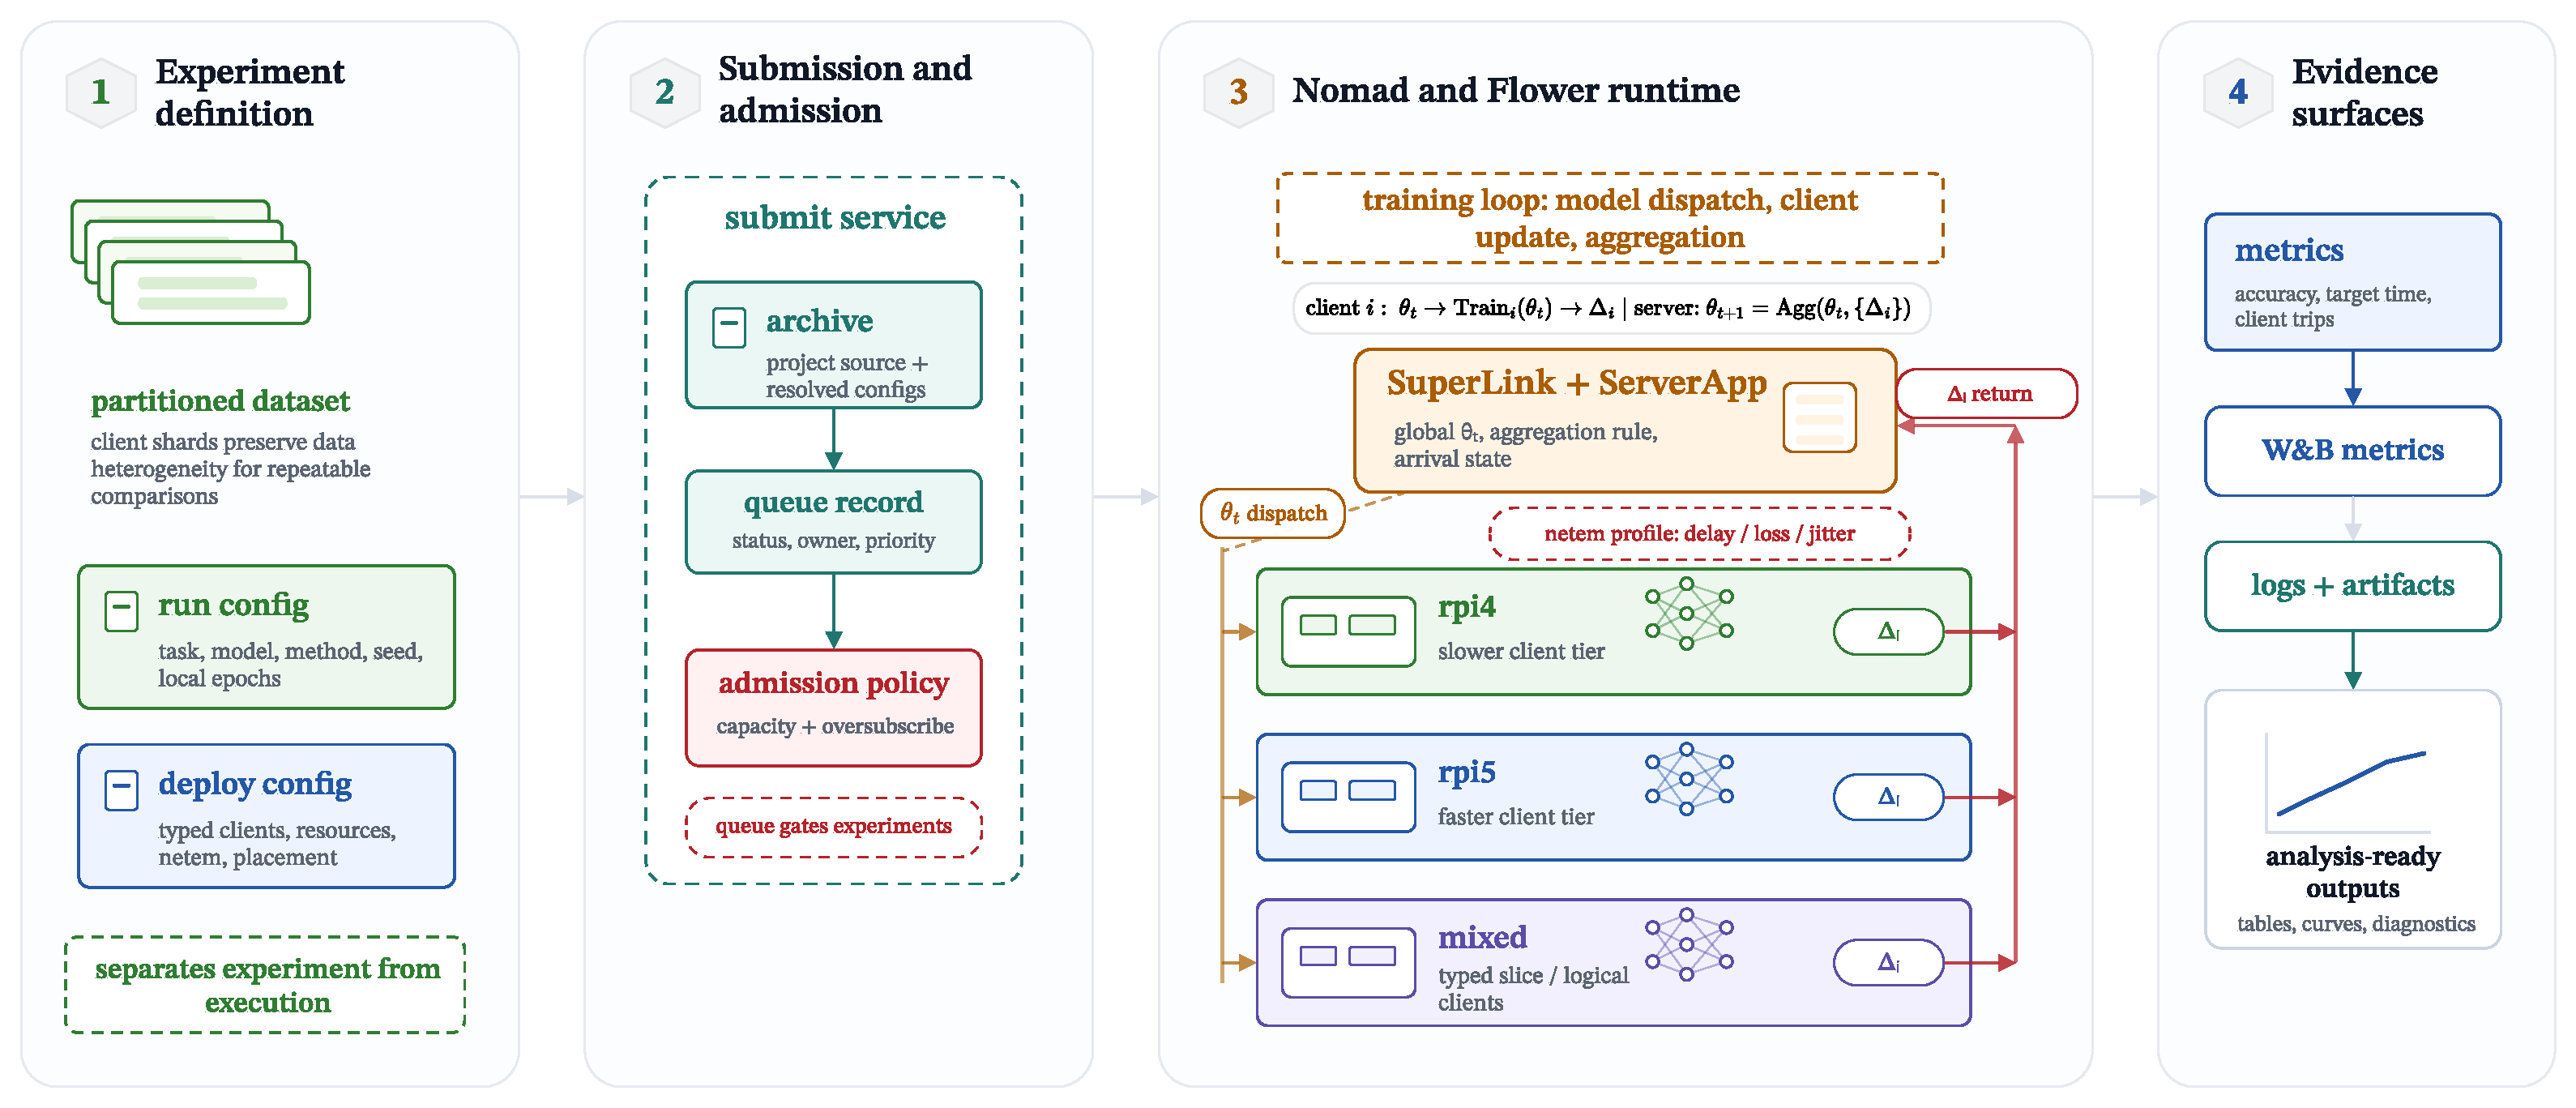
\includegraphics[width=\textwidth]{figures/remote_execution_lifecycle_clean.pdf}%
}
\caption{\textbf{Remote execution lifecycle.}}
\label{fig:remote_execution_lifecycle}
\end{figure}

The request records the Flower project, workload choices, deployment choices, and CLI overrides. The uploaded bundle makes it executable away from the developer machine. The \implterm{paletteGreen}{queue} stores the run persistently; admission checks typed capacity and placement constraints; and the \implterm{paletteGreen}{submit runner} invokes the deployment path: build or select the SuperExec image, render Nomad jobs, configure the Flower federation, and start \texttt{flwr run}. Metrics, \implterm{gray}{structured artifacts}, and \implterm{gray}{logs} then become evaluation evidence.

\FloatBarrier
\subsection[Submission interface]{Submission interface \impltaghead{implcomp:request}{paletteGreen}{cli}}

The \implterm{paletteGreen}{submit interface} is the user-facing control surface for remote experiments. \texttt{fedctl submit run} creates the submission; companion commands inspect status, logs, inventory, and results, and can cancel or purge terminal records. See the website \href{http://fedctl.cl.cam.ac.uk/help\#reference}{\underline{command reference}} (accessible via CL network) for the full command set.

For dissertation experiments, the typical launch form passes a Flower project, a run config \runconf, and a deploy config \deployconf:

\begin{codeblock}{bash}
fedctl submit run <flower-project> \
  --run-config <run-config> \
  --deploy-config <deploy-config>
\end{codeblock}

\paragraph{Request capture.}
The \implterm{paletteGreen}{CLI} inspects the Flower project, resolves the configs, applies overrides such as seed or run name, and records the reconstructed user-facing command.

\paragraph{Transport and executable environment.}
As part of creating a submission, the CLI uploads the project and resolved configuration material needed by the remote runner. The request can then execute from the submit node without depending on the developer machine. Transient build products and machine-local state are excluded from the bundle.

The \implterm{paletteGreen}{submit runner} \submitrunner{} builds or reuses the SuperExec image stored in the \implterm{paletteGreen}{registry} \regtag{}. When possible, the image tag is derived from the build context, Dockerfile, and Flower version, so identical inputs are reused across seed and method sweeps.

\FloatBarrier
\subsection[Queued admission and dispatch]{Queued admission and dispatch \impltaghead{implcomp:request}{paletteGreen}{svc}\impltaghead{implcomp:substrate}{fedstalebrown}{cluster}}
\label{sec:impl_queued_admission}

The \implterm{paletteGreen}{submit service} separates an experiment batch into persistent records and dispatch decisions. A \implterm{paletteGreen}{queue record} stores identity, artifact, runner arguments, priority, status, job mapping, and logs. A dispatcher reconciles queued records with live \implterm{fedstalebrown}{Nomad state}; an admitted record becomes a submit-runner Nomad batch job that downloads the bundle, reports job mappings, and enters the deployment path. Figure~\ref{fig:queue_admission_dispatch} visualises this step.

\begin{figure}[!htbp]
\centering
\makebox[\textwidth][c]{%
  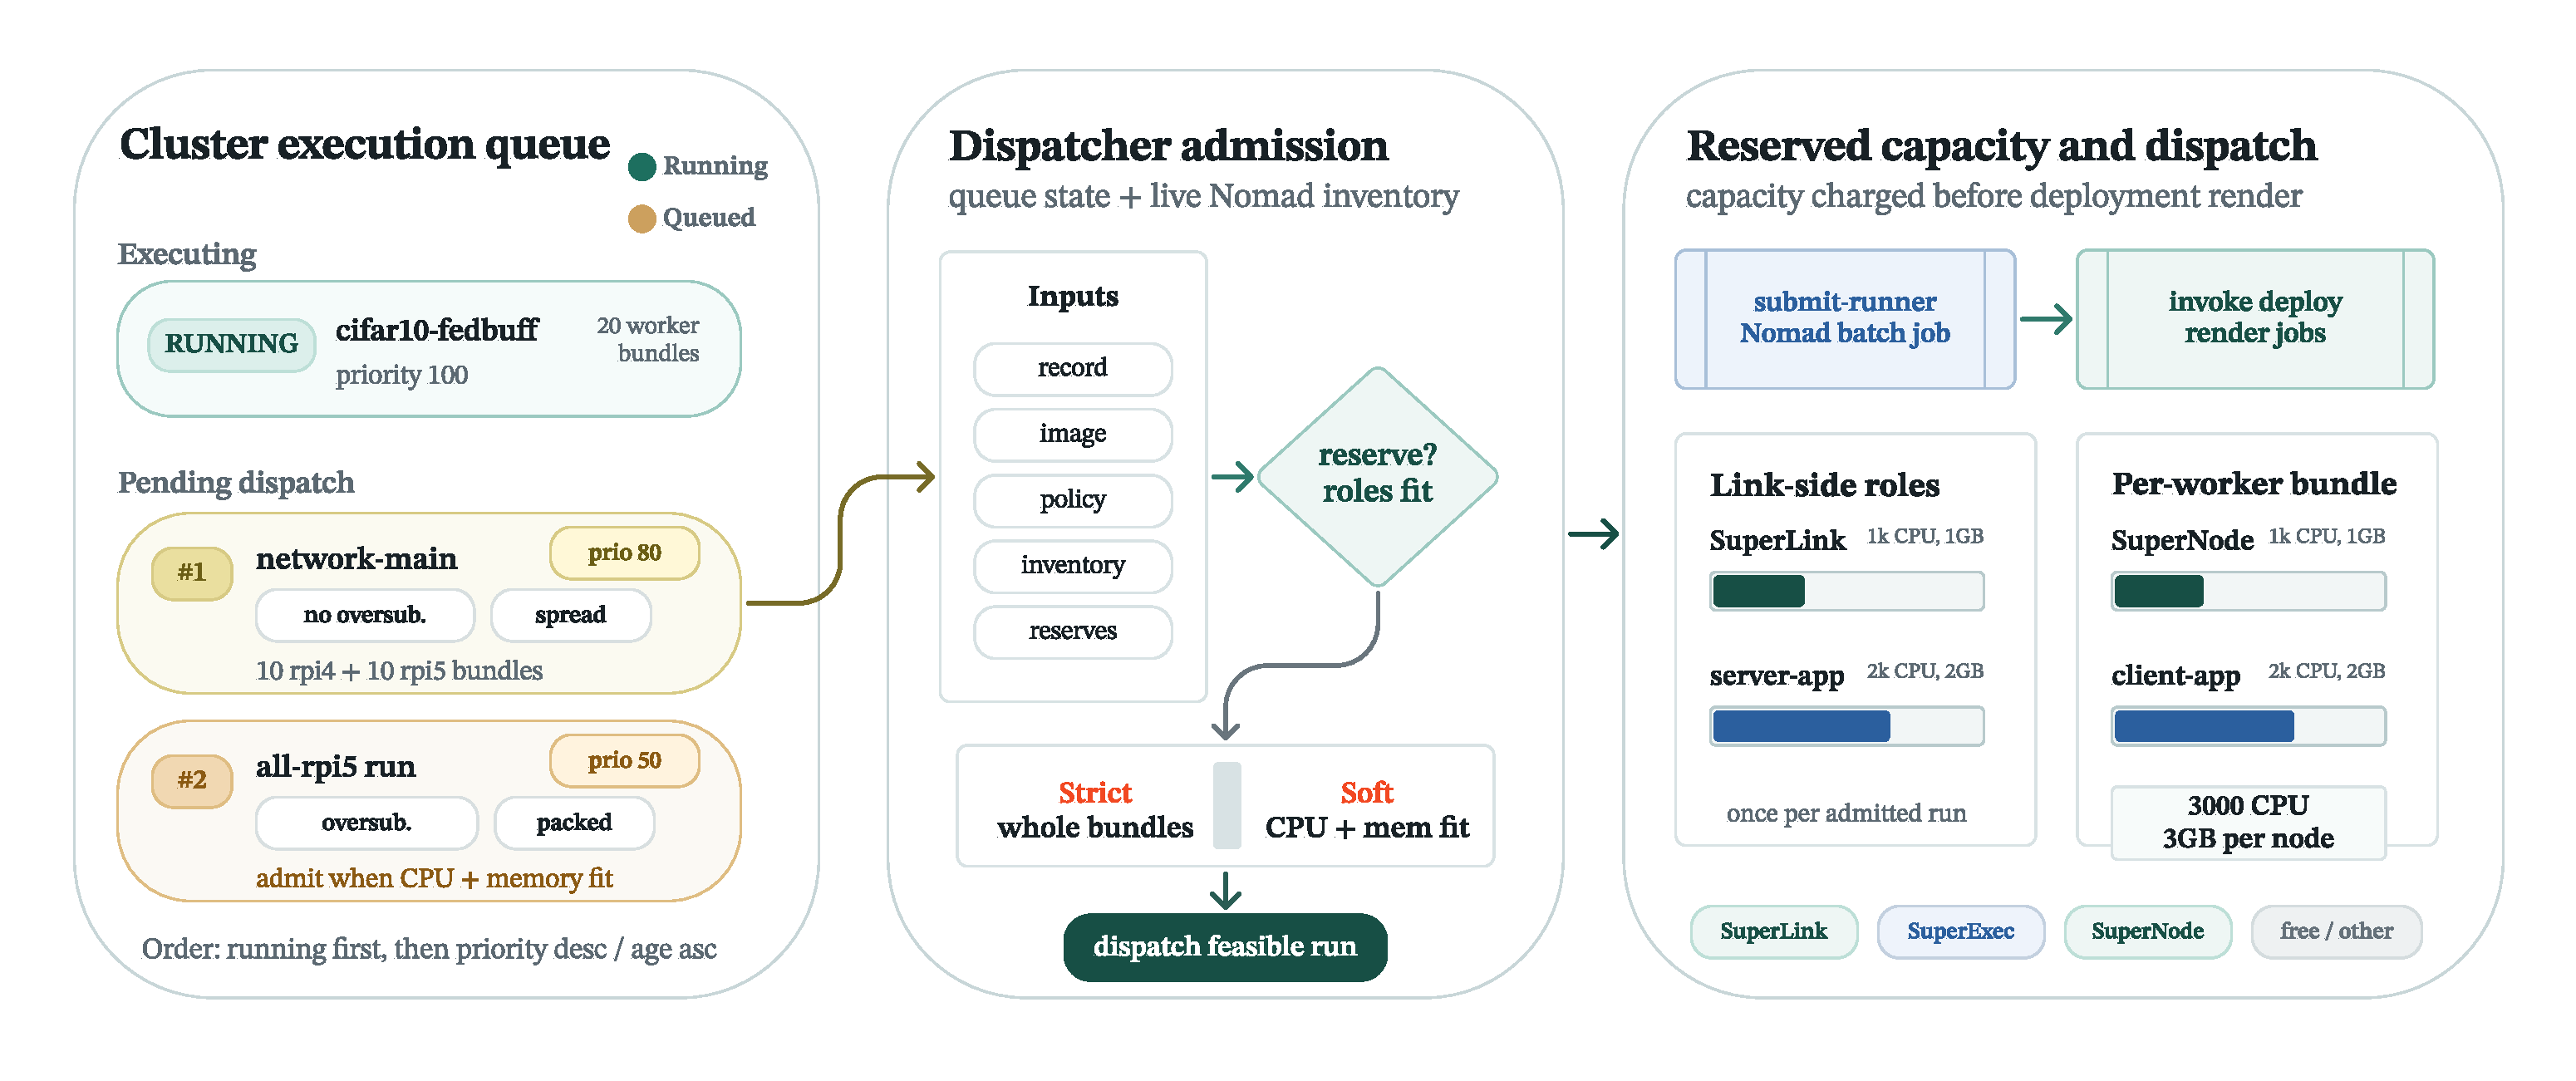
\includegraphics[width=1.08\textwidth]{figures/queue_admission_dispatch_clean.pdf}%
}
\caption{\textbf{Queued admission and dispatch path.}}
\label{fig:queue_admission_dispatch}
\end{figure}

% \begin{table}[!htbp]
% \centering
% \small
% \begin{tabularx}{\textwidth}{@{}>{\raggedright\arraybackslash}p{0.31\textwidth}>{\raggedright\arraybackslash}X@{}}
% \toprule
% \textbf{Admission input} & \textbf{How it is used} \\
% \midrule
% Submission record & Provides priority, namespace, submit image, artifact location, runner arguments, and current status. \\
% Runner arguments & Encode requested SuperNode counts, typed workers, and oversubscription policy. \\
% Deployment defaults & Provide resource reservations, node classes, and default placement policy when the request omits them. \\
% Nomad inventory & Supplies ready nodes, device type, node class, free CPU/memory, and visible allocations. \\
% Running submissions & Reserve capacity already consumed by active runs so later strict submissions do not collide with them. \\
% \bottomrule
% \end{tabularx}
% \caption{Inputs used by the submit-service dispatcher when deciding whether a queued run can be admitted.}
% \label{tab:submit_admission_inputs}
% \end{table}

\paragraph{Capacity and placement decision.}
Queueing is typed-capacity admission control. For strict deployments, the dispatcher accounts for whole typed worker bundles before dispatching, so a run requesting ten \texttt{rpi4} and ten \texttt{rpi5} workers waits until those devices are available. Placement can then either spread logical workers across distinct hosts, prefer spreading before reuse, or deliberately oversubscribe physical hosts.\footnote{These choices are controlled through the deploy config under \texttt{deploy.placement}, including \texttt{spread\_across\_hosts}, \texttt{prefer\_spread\_across\_hosts}, and \texttt{allow\_oversubscribe}.} Oversubscribed deployments use resource-based admission from live CPU and memory availability rather than exclusive device reservation, and the selected placement policy remains part of the recorded run state.

\FloatBarrier 
\subsection[Nomad rendering and service wiring]{Nomad rendering and service wiring \impltaghead{implcomp:deploy}{paletteGreen}{nomad}\impltaghead{implcomp:runtime}{paletteOrange}{roles}}

At this point, \texttt{fedctl} has a resolved deployment plan: the Flower roles to run, the device classes they should use, their resource reservations, and any network profiles. The \implterm{paletteGreen}{Nomad renderer} is the bridge from that plan to the cluster. It emits and submits the job specifications for SuperLink, SuperNodes, ServerApp, and ClientApps, starting the services first so their endpoints are discoverable before \texttt{flwr run} launches the application. Table~\ref{tab:nomad_flower_role_mapping} maps the Flower roles to the scheduler objects used in this deployment; Appendix~\ref{def:nomad} provides the Nomad vocabulary behind those objects.

\begin{table}[!htbp]
\centering
\small
{\renewcommand{\arraystretch}{1.18}
\begin{tabularx}{\textwidth}{@{}>{\raggedright\arraybackslash}p{0.16\textwidth}>{\raggedright\arraybackslash}p{0.28\textwidth}>{\raggedright\arraybackslash}X@{}}
\toprule
\textbf{Flower role} & \textbf{Nomad mapping} & \textbf{Purpose in the run} \\
\midrule
SuperLink & Link-class service job & Hosts the central Flower endpoints used by SuperNodes and the ServerApp. \\
SuperNodes & Service job with one task group per logical client & Provide client-side runtime endpoints; in \texttt{fedctl}, one endpoint is paired with each logical client and device placement. \\
ServerApp & Link-class service job & Runs the server application against the discovered SuperLink ServerApp endpoint. \\
ClientApp & One service job per logical client & Runs each client application against its paired SuperNode with client, device, and network metadata injected. \\
\bottomrule
\end{tabularx}
}
\caption{How the deployment renderer maps Flower runtime roles to Nomad jobs.}
\label{tab:nomad_flower_role_mapping}
\end{table}


% The control plane starts SuperLink first, then SuperNodes, then server-app and client-app SuperExec jobs. It writes the deployment manifest, configures the Flower project to use the remote federation, and invokes \texttt{flwr run <project> remote-deployment} with the materialized run config. Flower sees a normal remote deployment, while \texttt{fedctl} has already fixed placement, network, and service wiring.

\paragraph{Service discovery.}
Runtime addresses are injected through Nomad service definitions. SuperNodes discover the SuperLink service; the ServerApp receives the SuperLink ServerApp endpoint; and each ClientApp receives the corresponding SuperNode ClientApp endpoint. This makes the deployment robust to changing allocation IPs and ports across runs.

\paragraph{Runtime metadata.}
The renderer also injects experiment and placement metadata into the runtime. ClientApp containers receive the logical client index, device type, experiment identity, and, where strict placement is used, node identity. The research app \researchapp{} records this metadata with client metrics, which is what allows the evaluation to group training time, update share, and submodel quality by device class.

% Direct and queued runs converge on this downstream deployment path, so batch experiments and interactive debugging sessions exercise the same deployment code. The resulting operational state is exposed through the \implterm{gray}{submit-service UI and logs}, detailed in Appendix~\ref{appendix:observability_submit_ui}.


\FloatBarrier
\section{Controlling Real Hardware Heterogeneity}
\label{sec:impl_heterogeneity_control}

Hardware heterogeneity is inherent in a real edge cluster, but it must be controlled to support meaningful experiments. \texttt{fedctl} makes each client's hardware class and network conditions explicit at deployment time. Device-aware placement assigns logical clients to hardware classes; network impairment applies controlled communication conditions.

\FloatBarrier
\subsection[Device-aware placement]{Device-aware placement \impltaghead{implcomp:dep}{darkblue}{dep}\impltaghead{implcomp:deploy}{paletteGreen}{nomad}\impltaghead{implcomp:substrate}{fedstalebrown}{cluster}}

Device-aware placement exposes hardware heterogeneity as a declarative deployment variable. A run specifies \implterm{darkblue}{typed SuperNodes}, where each type corresponds to a hardware class such as \texttt{rpi4} or \texttt{rpi5}. Figure~\ref{fig:device_placement} traces this topology request to the device-labelled metrics used in the evaluation.

\begin{figure}[!htbp]
\centering
\makebox[\textwidth][c]{%
  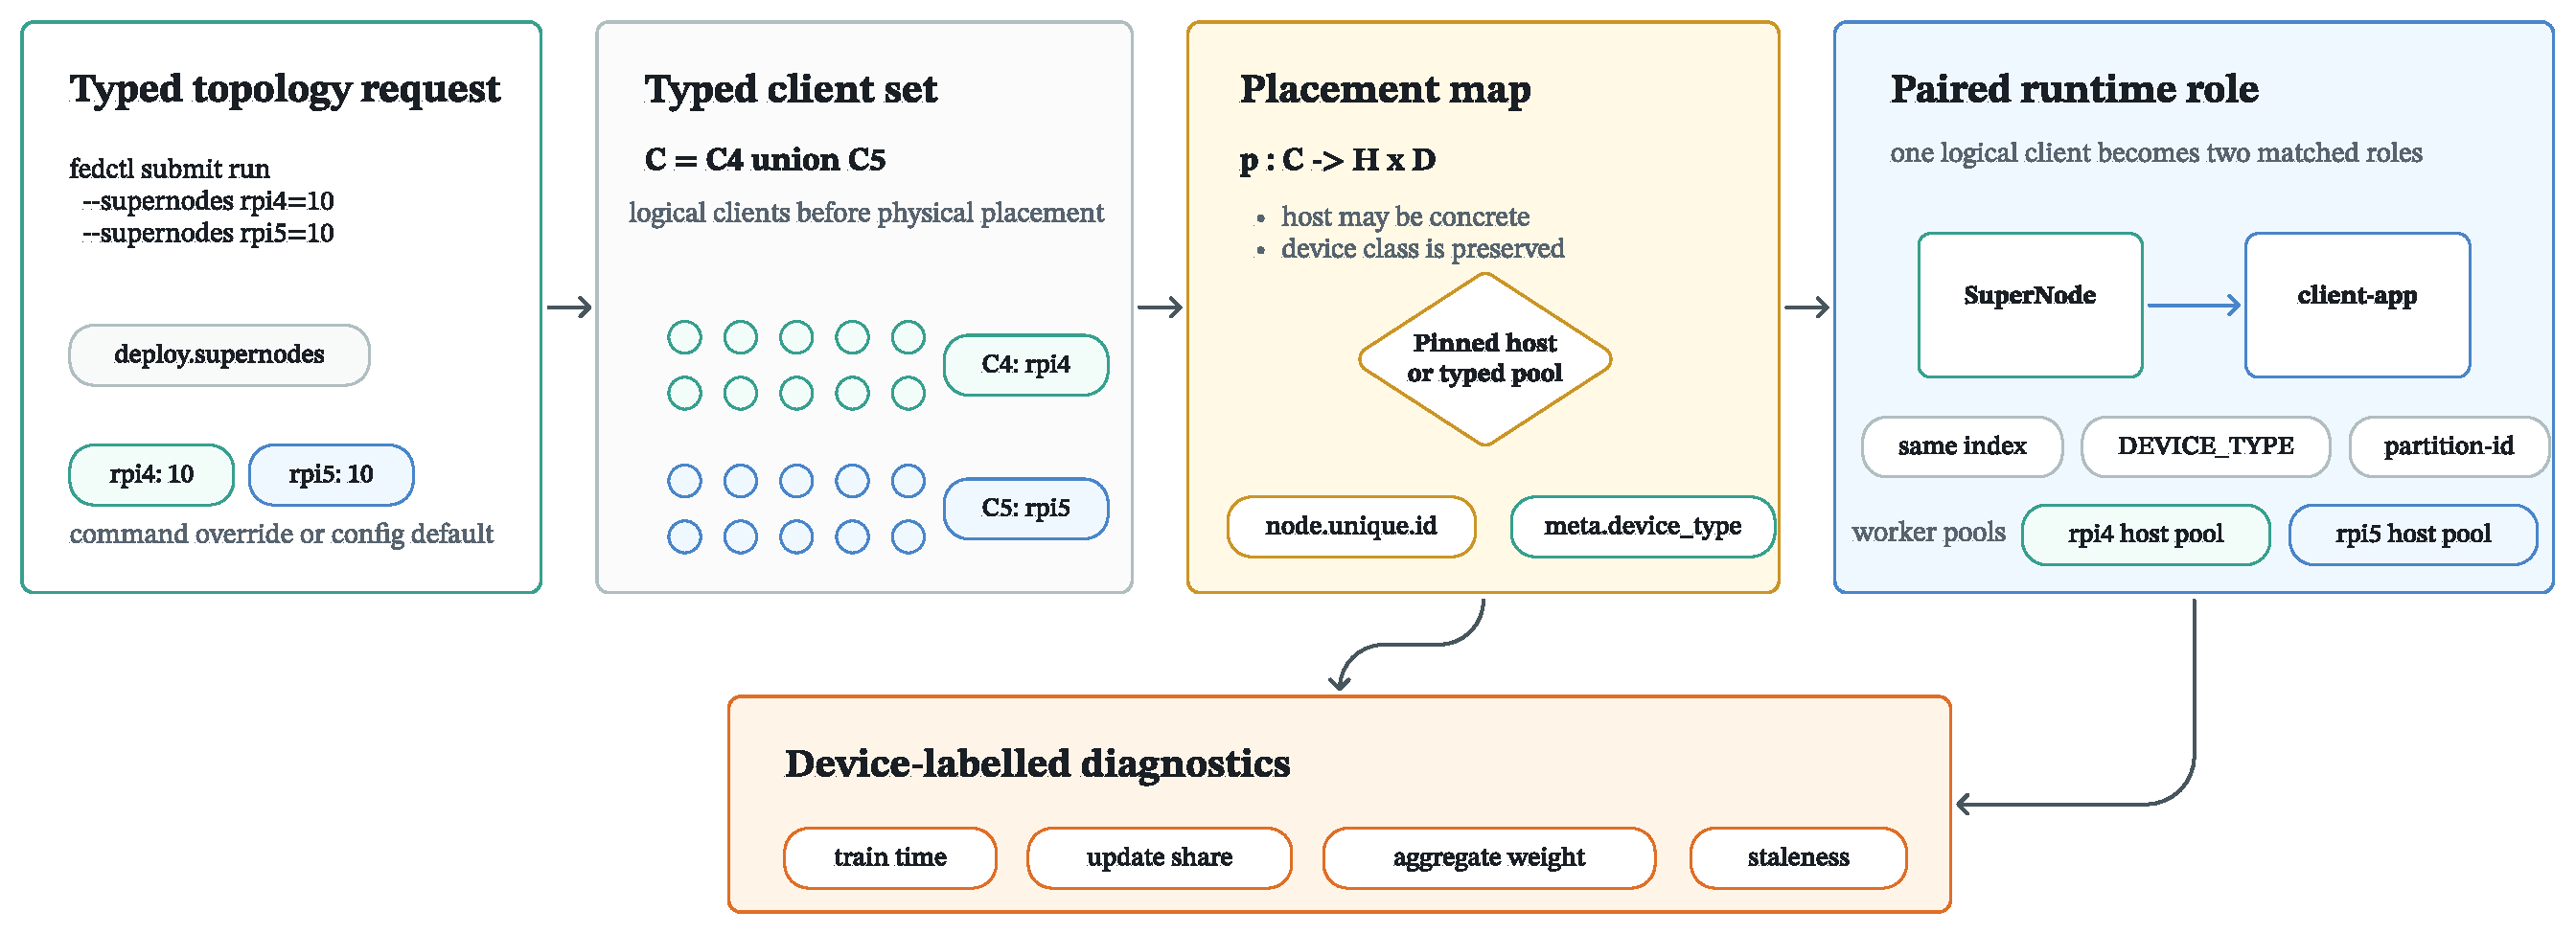
\includegraphics[width=\textwidth]{figures/device_placement_clean.pdf}%
}
\caption{\textbf{Device-aware placement and metadata flow.}}
\label{fig:device_placement}
\end{figure}

\paragraph{Typed SuperNodes.}
The interface is the \texttt{--supernodes} flag, which defines the logical topology as typed counts and overrides the deploy config \deployconf{} when present\footnote{If omitted, the same specification is read from \texttt{deploy.supernodes}. In both cases, the run records a typed SuperNode topology rather than a flat pool of interchangeable clients.}:
\begin{codeblock}{bash}
fedctl submit run <project>
  --supernodes rpi4=10, rpi5=10
\end{codeblock}


\paragraph{Deployment realisation.}
At deployment time, typed SuperNodes are mapped onto physical nodes by matching the requested type to \implterm{fedstalebrown}{Nomad node metadata}. Placement can be strictly pinned, constrained by device class, or expressed as a soft affinity. \footnote{It is enforced either by pinning to \texttt{node.unique.id} or by constraining \texttt{meta.device\_type}.}

\paragraph{Execution pairing.}
Each typed SuperNode is realised as a paired runtime: a Flower SuperNode communication endpoint and a corresponding client execution job. The pair shares a device-class constraint and a common instance index, so each logical SuperNode corresponds to exactly one communication endpoint and one execution context.

\paragraph{Evaluation linkage.}
Device type and instance identity are exposed to the application via environment variables, and are recorded with client metrics. This links deployment to evaluation: compute-heterogeneity experiments assign different model rates to \texttt{rpi4} and \texttt{rpi5}, while diagnostics such as training time, update share, aggregation weight, and staleness are analysed by device class.

\FloatBarrier
\subsection[Network impairment]{Network impairment \impltaghead{implcomp:dep}{darkblue}{dep}\impltaghead{implcomp:deploy}{paletteGreen}{nomad}}

Network impairment exposes communication heterogeneity as a deployment variable rather than a property of the FL method implementation. The deploy config \deployconf{} assigns a named impairment profile to each logical SuperNode. When a profile is active, \texttt{fedctl} renders the corresponding SuperNode task so that \texttt{flower-supernode} starts through a generated wrapper. The wrapper installs Linux traffic-control rules, verifies the resulting configuration, and then executes the normal SuperNode process. The research application and aggregation code therefore observe the same Flower runtime interface, while the deployment layer controls the network path.

\texttt{netem} is Linux's network-emulation facility for adding delay, jitter, packet loss, and bandwidth shaping; Appendix~\ref{def:network_evidence} gives the short definition used in this dissertation. Figure~\ref{fig:network_impairment} summarises the path from profile definition to logical assignment, Nomad rendering, wrapper setup, and ingress/egress enforcement.

\begin{figure}[!htbp]
\centering
\makebox[\textwidth][c]{%
  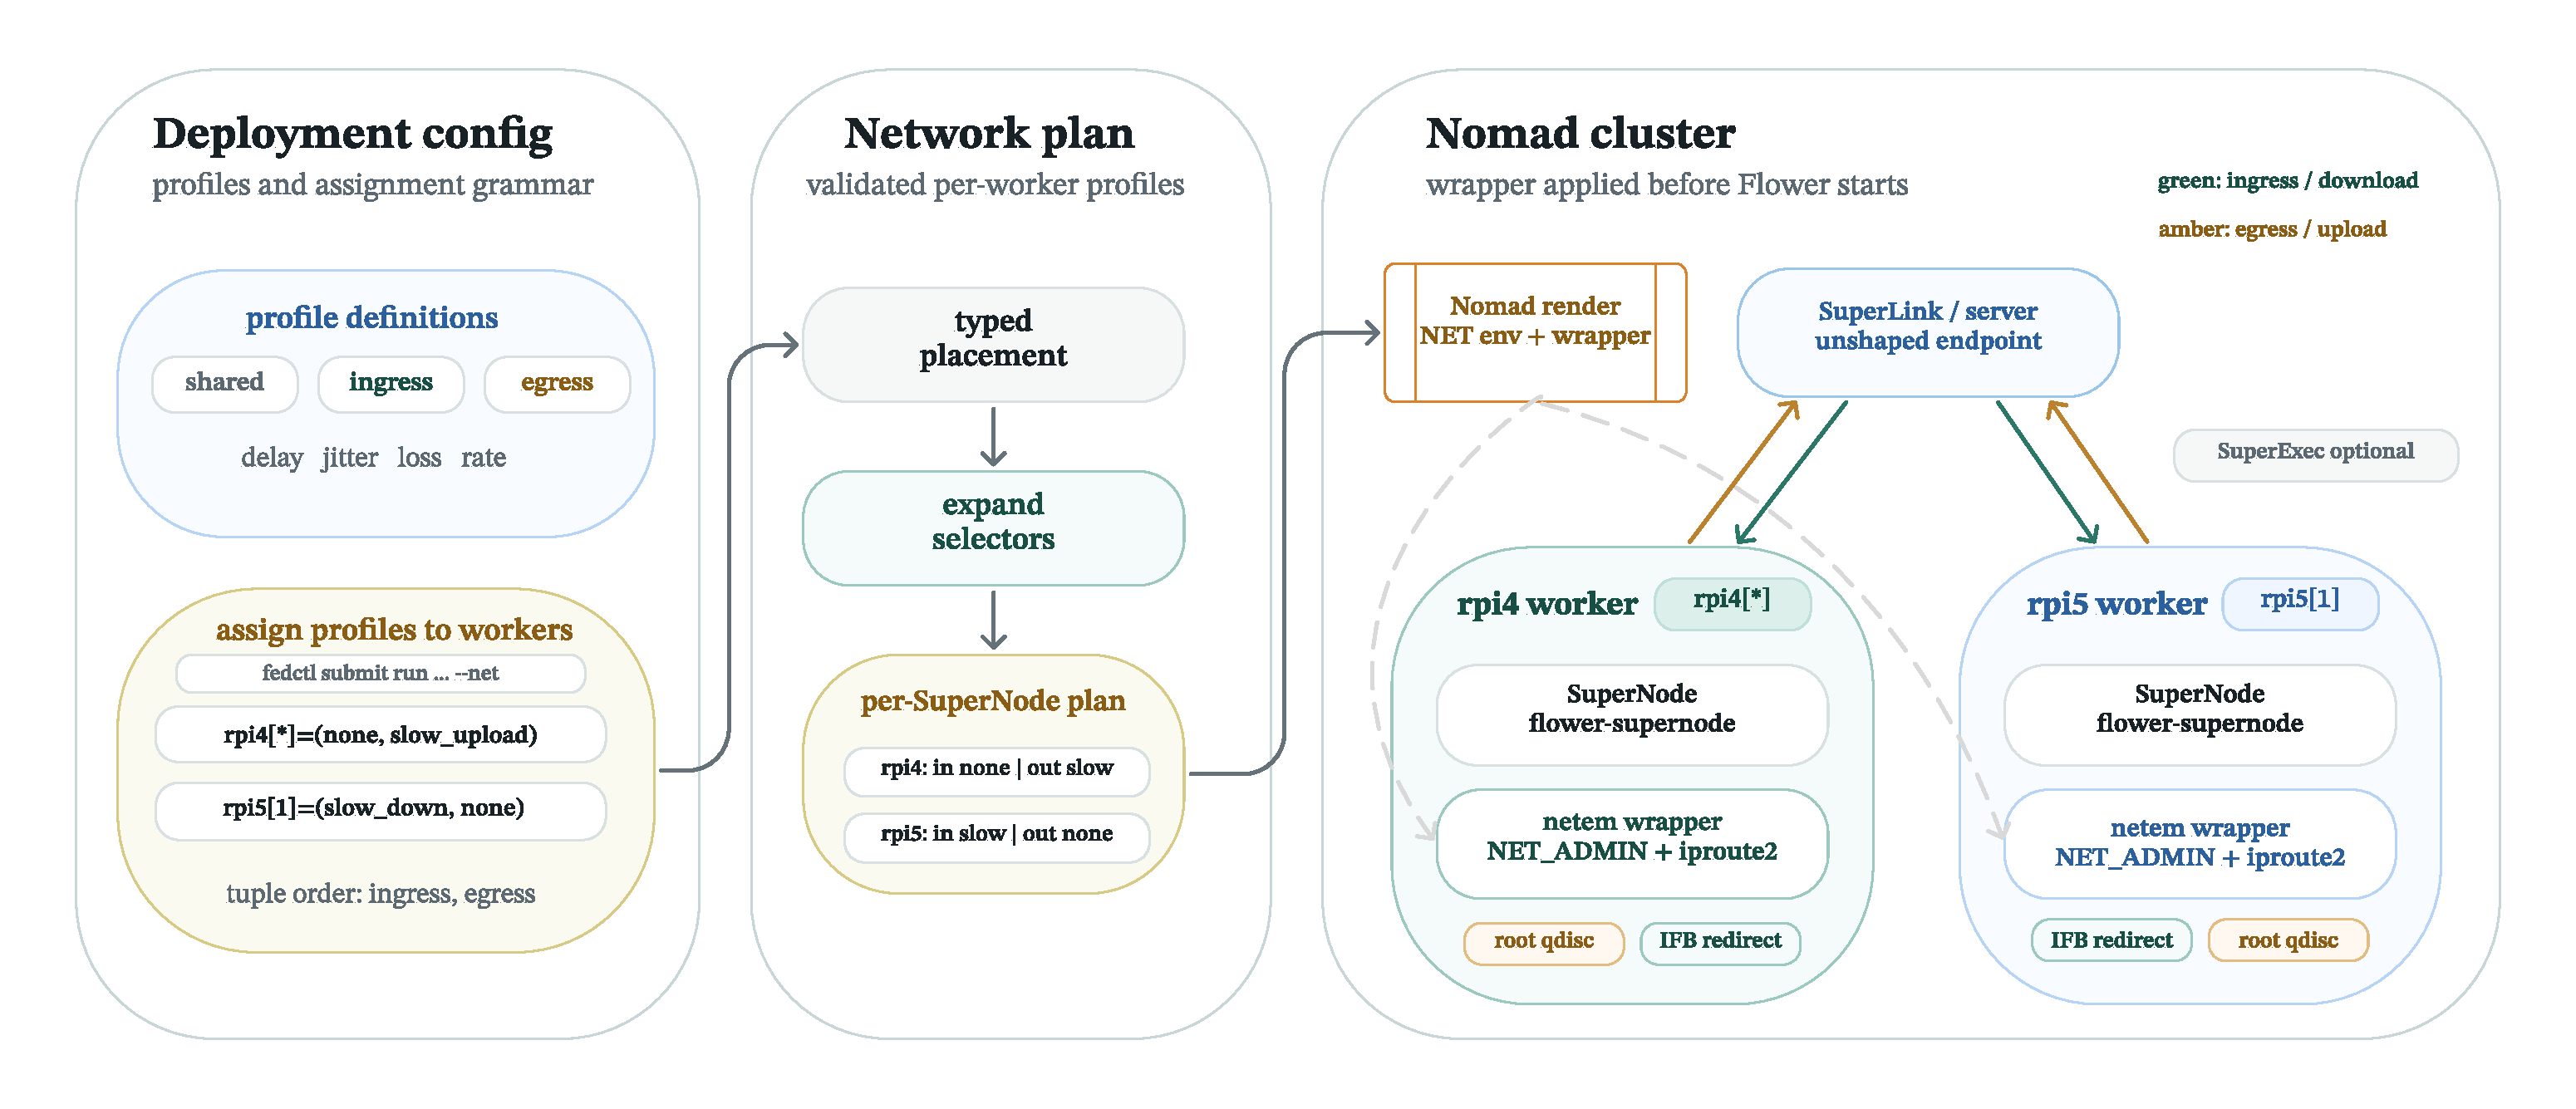
\includegraphics[width=1.08\textwidth]{figures/network_impairment_clean.pdf}%
}
\caption{\textbf{Network profile resolution and enforcement.}}
\label{fig:network_impairment}
\end{figure}

\paragraph{Profiles and assignment.}
A network profile is a named collection of traffic-shaping parameters consumed by the wrapper; \hyperlink{example:concrete-deploy-config}{\underline{the earlier deploy-config example}} gives one \texttt{mild} profile. Profiles may be symmetric or direction-specific, with \texttt{default\_profile} supplying the fallback when no explicit assignment is given. Assignments are resolved after typed placement, so selectors such as \texttt{rpi4[*]} or \texttt{rpi5[1]} refer to logical SuperNodes rather than physical hostnames. Direction-specific mappings use the tuple order \texttt{(ingress, egress)}, and the submit-time \texttt{--net} flag can override the deploy-config default.

\begin{table}[!htbp]
\centering
\small
\renewcommand{\arraystretch}{1.12}
\begin{tabularx}{\textwidth}{@{}>{\raggedright\arraybackslash}p{0.26\textwidth}>{\raggedright\arraybackslash}X@{}}
\toprule
\textbf{Parameter} & \textbf{Effect in the rendered task} \\
\midrule
\texttt{delay\_ms} & Adds base latency using \texttt{netem delay}. \\
\texttt{jitter\_ms} & Adds variation around the configured base latency. \\
\texttt{loss\_pct} & Drops the configured percentage of packets. \\
\texttt{rate\_mbit} & Adds a token-bucket bandwidth cap before delay/loss rules. \\
\texttt{rate\_latency\_ms} & Sets the token-bucket latency bound used with \texttt{rate\_mbit}. \\
\texttt{rate\_burst\_kbit} & Sets the token-bucket burst size used with \texttt{rate\_mbit}. \\
\bottomrule
\end{tabularx}
\caption{Traffic-shaping parameters consumed by the network-impairment wrapper. The same fields can define symmetric profiles or separate ingress and egress profiles.}
\label{tab:impl_network_profiles}
\end{table}

\paragraph{Wrapper enforcement.}
At deployment time, \texttt{fedctl} validates the selected profiles, expands typed selectors, and renders each affected SuperNode task to run as \texttt{root} with Docker \texttt{NET\_ADMIN}. The task receives \texttt{NET\_*} variables and starts through the generated wrapper script. Egress impairment attaches \texttt{tc qdisc} rules directly to the task interface. Ingress impairment redirects packets through an \texttt{ifb} device before applying the same token-bucket and \texttt{netem} controls. The wrapper then \texttt{exec}s \texttt{flower-supernode}, so the deployed FL application continues to use the normal Flower interface.

% \paragraph{Experimental scope.}
% The reported network experiments apply impairment at the SuperNode role. This targets the communication path between logical clients and the Flower federation while keeping server and client application code unchanged. The same wrapper mechanism could also be enabled for ServerApp or ClientApp SuperExec roles, but those extensions are not used in the dissertation experiments.

\FloatBarrier
\section{Flower Application and Method Layer}
\label{sec:impl_flower_application}

The dissertation-specific FL logic is implemented in the \implterm{paletteOrange}{research app} \researchapp{}. It resolves run configs, constructs tasks and models, loads partitions, executes local client work, coordinates server-side methods, and records method-level outputs. Figure~\ref{fig:application_method_layer} shows the boundary between deployment metadata, shared server/client task code, and the evidence consumed by Chapter~\ref{chap:evaluation}.

\begin{figure}[!htbp]
\centering
\makebox[\textwidth][c]{%
  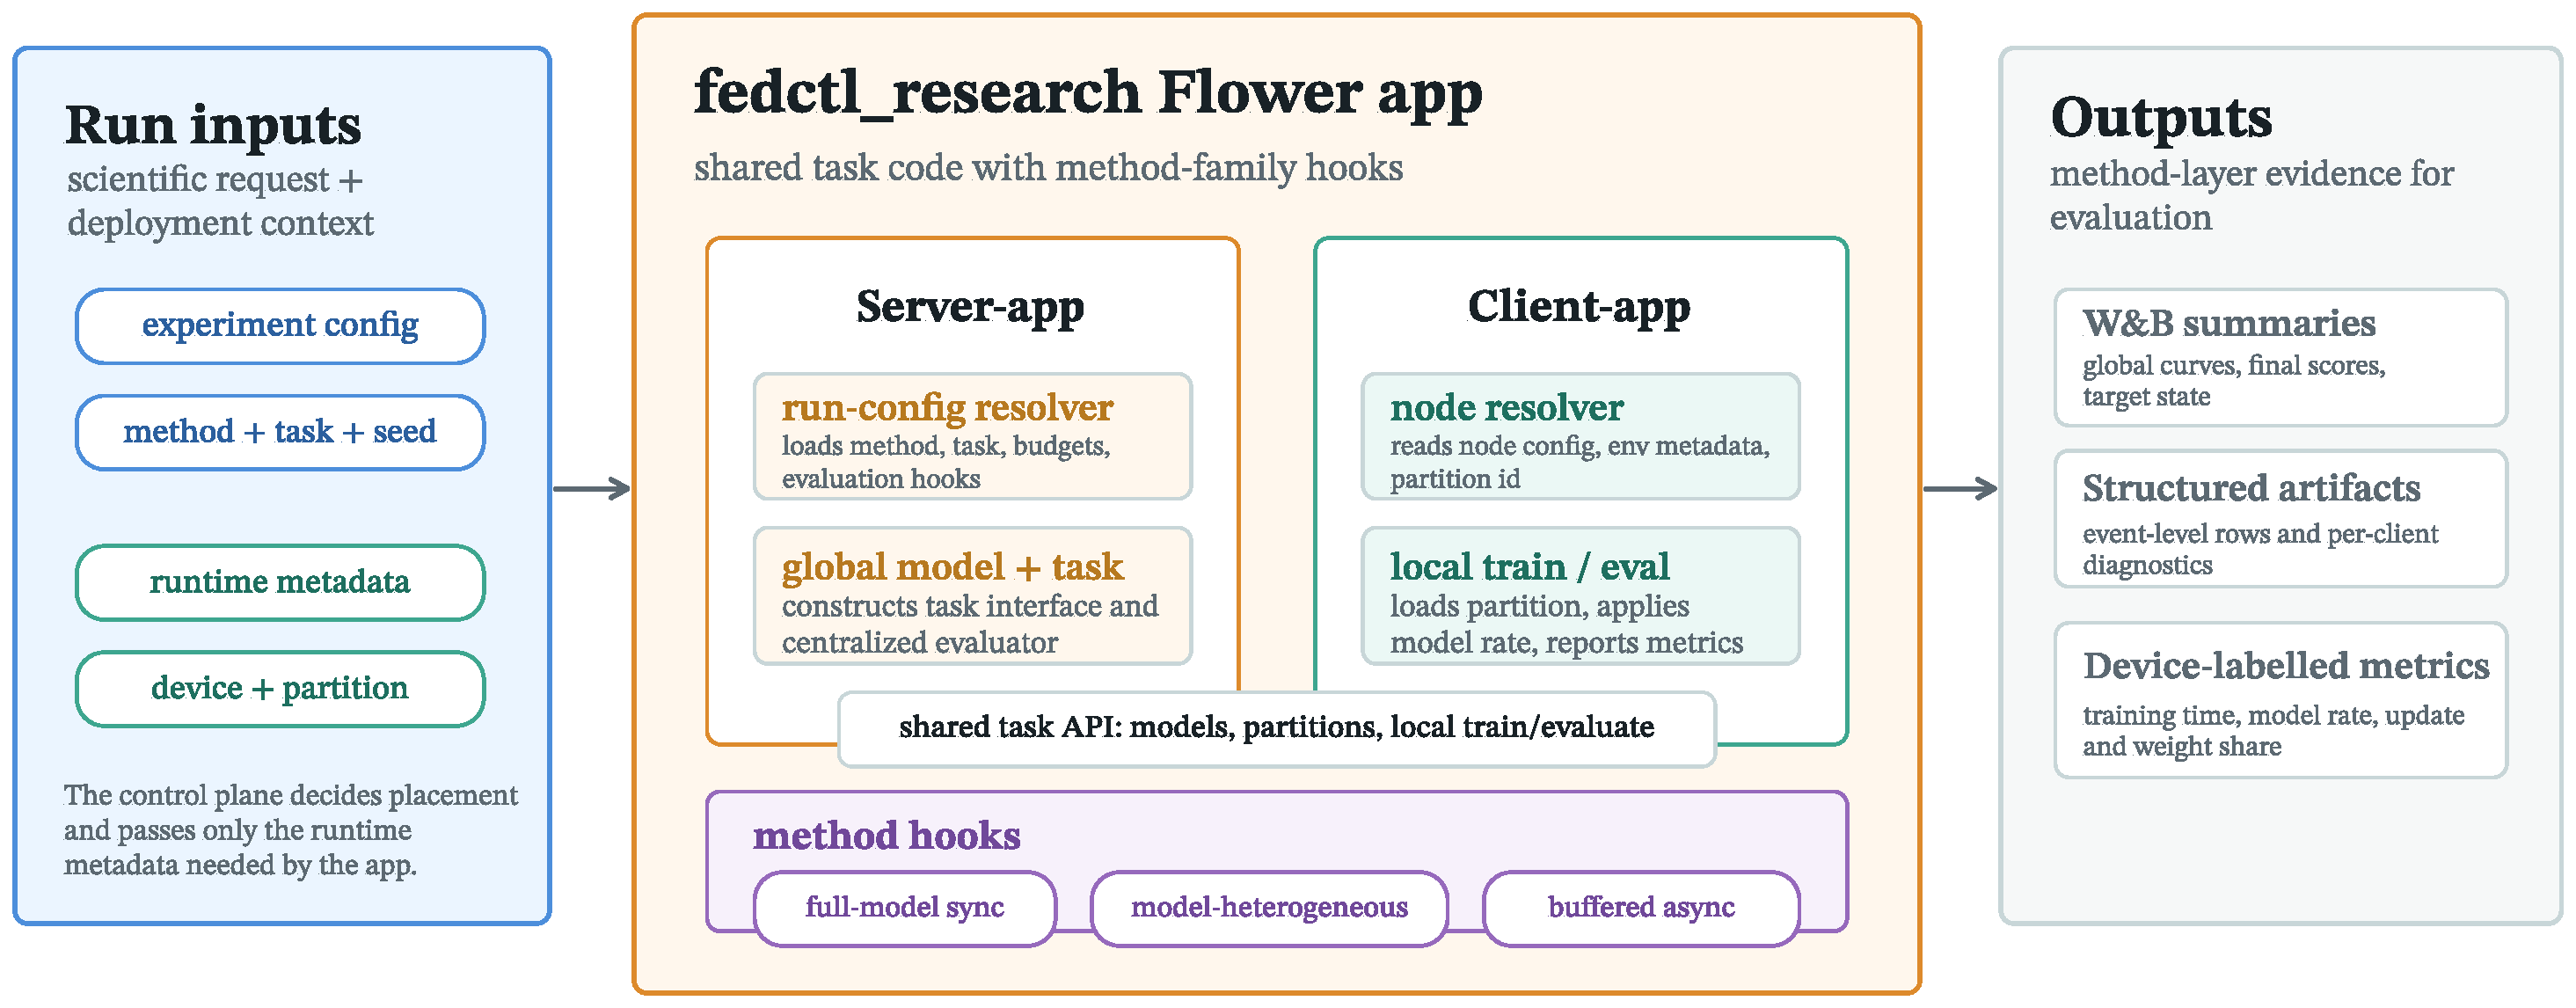
\includegraphics[width=\textwidth]{figures/application_method_layer.pdf}%
}
\caption{\textbf{Research application and method layer.}}
\label{fig:application_method_layer}
\end{figure}

\subsection[Research-app interface]{Research-app interface \impltaghead{implcomp:runtime}{paletteOrange}{app}}

The server and client entry points share one task interface. A run config selects the task, model, partitioner, method, optimizer settings, local budget, and evaluation path; the task implementation then supplies model construction, partition loading, local training, local evaluation, and centralized evaluation. Appendix~\ref{appendix:evaluation_tasks} summarises the evaluation datasets and task models instantiated through this interface.

Clients return updated parameters together with loss, example count, timing, throughput, device type, model rate, and partition identity. The server records target attainment, centralized evaluation, asynchronous staleness, accepted-update metadata, and method-specific diagnostics. This evidence path is what lets Chapter~\ref{chap:evaluation} relate accuracy, runtime, submodel quality, and slow-device influence back to the deployment choices fixed by \texttt{fedctl}.

\FloatBarrier
\subsection{Implemented method families}

The method layer implements the families evaluated in Chapter~\ref{chap:evaluation}. Chapter~\ref{chap:related_work} gives prior-method context, and Appendix~\ref{appendix:algorithms} gives unified pseudocode; here the emphasis is on the implementation distinctions needed for deployed experiments.

\paragraph{Full-model synchronous training.}
\texttt{FedAvg} is the full-model synchronous baseline. The server broadcasts the same global model to selected clients, waits for the configured replies, and aggregates returned models by example count.

\paragraph{Submodel training.}
\texttt{HeteroFL}, \texttt{FedRolex}, and \texttt{FIARSE} share one partial-training pipeline: select the client-visible parameter subset, train locally, scatter returned updates back into the global model, and aggregate only covered regions. They differ in the selection rule: fixed nested slices for \texttt{HeteroFL}, rolling windows for \texttt{FedRolex}, and sparse importance masks for \texttt{FIARSE}. \texttt{FIARSE} follows the paper's sparse-mask training mechanism, but executes those masks through dense PyTorch kernels on worker CPUs, so improved submodel quality does not necessarily translate into measured wall-clock speedup.

\paragraph{Buffered asynchronous training.}
\texttt{FedBuff} and \texttt{FedStaleWeight} use a custom buffered asynchronous server loop so the implementation can control in-flight concurrency, buffering, staleness, and accepted-update logging. \texttt{FedStaleWeight} changes only the buffer weighting rule, using the stale-aware weighting described in Section~\ref{sec:fedstaleweight_related}. The server records both update share and weight share, separating arrival frequency from aggregate influence.

\paragraph{Asynchronous submodel FL.}
\texttt{FedCover} combines the buffered asynchronous loop with HeteroFL-style nested submodels. Each reply carries its model rate and trained parameter slice, allowing the server to scatter the returned delta into the global parameter space and measure which parameters were covered. Section~\ref{sec:fedcover_impl} introduces the resulting coverage-aware aggregation algorithm.

\FloatBarrier
\section{\texttt{FedCover}: Coverage-Aware Buffered Aggregation}
\label{sec:fedcover_impl}

This section defines \texttt{FedCover} for asynchronous submodel FL, the setting introduced in Section~\ref{sec:async_submodel_related}. The base path combines \texttt{FedBuff}-style buffering with \texttt{HeteroFL}-style nested slicing; \texttt{FedCover} keeps that path and adds only a capped inverse-coverage correction to each aggregated parameter delta.

\paragraph{Buffered submodel replies.}
At server step \(s\), let \(\mathcal{B}_s\) be the accepted buffer, let \(\alpha_i\) be the stale-update weight for reply \(i\), and let \(I_i\) be the submodel parameter set trained by that reply. The shared asynchronous sign convention is \(\Delta_i=w^{[v_i]}-\tilde{w}_i\), with local component \(\Delta_{i,j}\) defined when \(j \in I_i\).

\paragraph{Parameter-level coverage.}
The buffered partial-model delta for parameter \(j\) is
\[
    \bar{\Delta}_j^{[s]}
    =
    \sum_{i \in \mathcal{B}_s}
    \alpha_i \mathbf{1}[j \in I_i]\Delta_{i,j}.
\]
FedCover also measures the observed coverage mass,
\[
    c_j^{[s]} =
    \sum_{i \in \mathcal{B}_s}
    \alpha_i \mathbf{1}[j \in I_i].
\]
The weights \(\alpha_i\) are normalized over the accepted buffer, so \(0 \le c_j^{[s]} \le 1\). The coverage mass is the stale-weighted accepted mass whose submodel contains \(j\), not a count of buffered replies. Thus, under-covered parameters receive a smaller effective update even when the buffer itself is full.

\paragraph{Inverse-coverage gain.}
Figure~\ref{fig:fedcover_coverage_gain} illustrates coverage mass for one parameter and the resulting gain curve.

\begin{figure}[!htbp]
\centering
\begin{adjustbox}{max width=\textwidth}
\begin{tikzpicture}[
  font=\scriptsize,
  >=Latex,
  cell/.style={minimum width=1.06cm, minimum height=0.58cm, draw=gray!45, line width=0.3pt, align=center},
  covered/.style={cell, fill=paletteGreen!16, draw=paletteGreen!65!black, text=paletteGreen!35!black},
  missing/.style={cell, fill=gray!7, draw=gray!40, text=gray!60},
  note/.style={align=center, text=gray!75!black},
  paneltitle/.style={font=\small\bfseries, align=center}
]
  \node[paneltitle] at (2.55,3.85) {Accepted buffer for one parameter \(j\)};
  \node[note] at (2.55,3.42) {\(\sum_{i\in\mathcal{B}_s}\alpha_i=1\), but not every reply covers \(j\)};

  \node[anchor=east, font=\scriptsize\bfseries] at (-0.70,2.74) {reply};
  \node[anchor=east, font=\scriptsize\bfseries] at (-0.70,2.06) {\(\alpha_i\)};
  \node[anchor=east, font=\scriptsize\bfseries] at (-0.70,1.38) {covers \(j\)};

  \foreach \x/\name/\weight/\state in {
    0/{1}/0.25/yes,
    1.18/{2}/0.20/no,
    2.36/{3}/0.20/yes,
    3.54/{4}/0.20/no,
    4.72/{5}/0.15/yes
  } {
    \node[cell, fill=gray!3] at (\x,2.74) {\(i=\name\)};
    \node[cell, fill=gray!3] at (\x,2.06) {\(\weight\)};
  }
  \node[covered] at (0,1.38) {yes\\\(+0.25\)};
  \node[missing] at (1.18,1.38) {no\\\(+0\)};
  \node[covered] at (2.36,1.38) {yes\\\(+0.20\)};
  \node[missing] at (3.54,1.38) {no\\\(+0\)};
  \node[covered] at (4.72,1.38) {yes\\\(+0.15\)};

  \draw[->, line width=0.5pt, paletteGreen!80!black]
    (2.36,0.80) -- (2.36,0.24);
  \node[
    rounded corners=2pt,
    draw=paletteGreen!60!black,
    fill=paletteGreen!8,
    align=center,
    inner sep=4pt,
    minimum width=4.8cm
  ] at (2.36,-0.32)
    {\(c_j^{[s]}=0.25+0.20+0.15=0.60\)\\observed coverage mass};

  \draw[gray!35, line width=0.4pt] (6.35,-0.80) -- (6.35,4.05);

  \node[paneltitle] at (10.25,3.85) {Capped inverse-coverage gain};
  \node[note] at (10.25,3.42) {example: \(\gamma=0.5,\ \kappa_{\max}=2\), so \(c_{\mathrm{cap}}=\kappa_{\max}^{-1/\gamma}=0.25\)};

  \coordinate (origin) at (8.05,0.10);
  \draw[->, line width=0.45pt] (origin) -- (12.65,0.10);
  \draw[->, line width=0.45pt] (origin) -- (8.05,2.80)
    node[above, font=\scriptsize] {\(\kappa(c)\)};

  \foreach \cx/\lab in {0/{0},0.25/{\(c_{\mathrm{cap}}\)},0.60/{0.60},1/{1}} {
    \draw[gray!55] ({8.05+4.15*\cx},0.10) -- ({8.05+4.15*\cx},0.00);
    \node[below, font=\scriptsize] at ({8.05+4.15*\cx},0.09) {\lab};
  }
  \foreach \ky/\lab in {1/{1},1.29/{1.29},2/{2}} {
    \draw[gray!55] (8.05,{0.10+2.25*(\ky-1)}) -- (7.95,{0.10+2.25*(\ky-1)});
    \node[left, font=\scriptsize] at (7.91,{0.10+2.25*(\ky-1)}) {\lab};
  }

  \draw[gray!20, line width=0.25pt] (8.05,0.10) grid[xstep=0.83, ystep=0.5625] (12.20,2.35);
  \draw[paletteOrange!90!black, very thick]
    plot[domain=0:0.25, samples=2] ({8.05+4.15*\x},{0.10+2.25});
  \draw[paletteOrange!90!black, very thick]
    plot[domain=0.25:1, samples=70] ({8.05+4.15*\x},{0.10+2.25*(1/sqrt(\x)-1)});

  \draw[dashed, paletteGreen!80!black]
    ({8.05+4.15*0.60},0.10) -- ({8.05+4.15*0.60},{0.10+2.25*(1/sqrt(0.60)-1)});
  \draw[dashed, paletteGreen!80!black]
    (8.05,{0.10+2.25*(1/sqrt(0.60)-1)}) -- ({8.05+4.15*0.60},{0.10+2.25*(1/sqrt(0.60)-1)});
  \fill[paletteGreen!80!black] ({8.05+4.15*0.60},{0.10+2.25*(1/sqrt(0.60)-1)}) circle (1.8pt);
  \node[
    rounded corners=2pt,
    draw=paletteGreen!60!black,
    fill=paletteGreen!8,
    align=center,
    inner sep=3pt,
    anchor=west
  ] at (10.75,1.33) {\(c=0.60\)\\\(\kappa=0.60^{-0.5}=1.29\)};

  \node[align=center, text=gray!75!black] at (10.10,-0.50) {observed coverage mass \(c\)};
  \node[anchor=north west, align=left, text=gray!75!black] at (8.00,-0.78)
    {\(\kappa(c)=\min(\kappa_{\max},c^{-\gamma})\), applied only when \(c>0\)};
\end{tikzpicture}
\end{adjustbox}
\caption{FedCover converts partial-model coverage into an inverse-coverage gain. The left panel shows one accepted buffer in which parameter \(j\) is present in only three replies, giving \(c_j^{[s]}=0.60\). The right panel shows the corresponding gain curve for an illustrative hyperparameter choice; the flat region is the gain cap, not an additional coverage threshold.}
\label{fig:fedcover_coverage_gain}
\end{figure}

Under nested submodels, shared prefix parameters have high coverage mass, while outer blocks used only by larger model rates have lower coverage mass. The server converts coverage mass directly into a capped inverse-coverage gain,
\[
    \kappa_j^{[s]}
    =
    \min\!\left(\kappa_{\max}, (c_j^{[s]})^{-\gamma}\right)
    \quad \text{for } c_j^{[s]} > 0.
\]

\paragraph{Corrected server update.}
The server applies
\[
    w_j^{[s+1]}
    =
    w_j^{[s]} - \eta_s \kappa_j^{[s]}\bar{\Delta}_j^{[s]}
    \quad \text{when } c_j^{[s]} > 0,
\]
and leaves \(w_j\) unchanged when the buffer contains no update for that parameter. The correction only rescales parameters that appear in the accepted buffer; it does not impute updates for parameters with \(c_j^{[s]}=0\). Full coverage gives \(\kappa_j^{[s]}=1\); lower coverage increases the update by an inverse-coverage factor, with \(\gamma\) controlling the correction strength and \(\kappa_{\max}\) preventing excessive amplification. If all clients train the full model, \texttt{FedCover} reduces to ordinary buffered asynchronous aggregation; setting \(\gamma=0\) recovers the coverage-disabled asynchronous \texttt{HeteroFL} baseline.

\FloatBarrier
% \section{Repository Organisation}
% \label{sec:impl_repo_overview}

% Figure~\ref{fig:repo_overview} maps the implementation mechanisms to the repository.

% \begin{figure}[!htbp]
% \centering
% \begin{adjustbox}{max width=\textwidth}
% \begin{minipage}{0.92\textwidth}
% \footnotesize
% \renewcommand*\DTstyle{\ttfamily}
% \renewcommand*\DTstylecomment{\normalfont\scriptsize\color{gray}}
% \DTsetlength{0.2em}{1.0em}{0.25em}{0.35pt}{1.2pt}
% \dirtree{%
% .1 fedctl/.
% .2 \textcolor{darkblue}{src/fedctl/}\DTcomment{generic control plane}.
% .3 \textcolor{darkblue}{commands/}\DTcomment{CLI entry points}.
% .3 \textcolor{darkblue}{build/}\DTcomment{image construction and reuse}.
% .3 \textcolor{darkblue}{deploy/}\DTcomment{Nomad planning, rendering, placement, netem}.
% .3 \textcolor{darkblue}{submit/}\DTcomment{submit-runner and artifact reporting}.
% .2 \textcolor{paletteGreen}{submit\_service/}\DTcomment{queue, dispatcher, UI, inspection APIs}.
% .2 \textcolor{fedrolexpurple}{apps/fedctl\_research/}\DTcomment{dissertation Flower app}.
% .3 \textcolor{fedrolexpurple}{src/fedctl\_research/}\DTcomment{tasks, methods, runtime, artifacts}.
% .3 \textcolor{fedrolexpurple}{run\_configs/}\DTcomment{Flower run-config definitions}.
% .3 \textcolor{fedrolexpurple}{deploy\_configs/}\DTcomment{deploy config presets used by fedctl}.
% .2 \textcolor{paletteOrange}{templates/}\DTcomment{Nomad and submit-runner templates}.
% .2 \textcolor{paletteOrange}{ansible/}\DTcomment{cluster provisioning}.
% .2 \textcolor{paletteOrange}{plot/}\DTcomment{figure/table generation}.
% .2 \textcolor{paletteOrange}{writeup/}\DTcomment{dissertation source and figures}.
% }
% \end{minipage}
% \end{adjustbox}
% \caption{\textbf{\texttt{fedctl} repository organisation.}}
% \label{fig:repo_overview}
% \end{figure}

% \texttt{src/fedctl} contains the \implterm{darkblue}{CLI and control-plane code} for packaging, building, deploying, submitting, and inspecting Flower workloads. \texttt{submit\_service} is the \implterm{paletteGreen}{queue, dispatcher, UI, and inspection layer}. \texttt{apps/fedctl\_research} is the \implterm{fedrolexpurple}{dissertation FL logic}: tasks, partitioners, methods, runtime helpers, run configs, deploy config presets, and result artifacts. \texttt{plot} and \texttt{writeup} support reproducible figures and thesis artifacts.

% Overall, the implementation turns heterogeneous worker hardware into an explicit experimental platform. The configuration split separates workload choices from execution conditions; the control plane packages and deploys runs reproducibly; typed placement and network profiles control compute heterogeneity and straggler-induced heterogeneity; and the research application emits the metrics used in Chapter~\ref{chap:evaluation}.

% !TeX root = main.tex
\chapter{Evaluation}
\label{chap:evaluation}

\providecommand{\evalqanchor}[1]{\hypertarget{eval:#1}{\textbf{#1}}}
\providecommand{\evalqref}[1]{\hyperlink{eval:#1}{\textbf{#1}}}

This chapter uses \texttt{fedctl} to evaluate heterogeneous FL methods under real hardware and network effects rather than abstract delay or capacity models. The evaluation considers three complementary axes. First, compute heterogeneity asks whether weaker devices should train smaller subnetworks. Second, straggler-induced heterogeneity asks whether asynchronous coordination reduces time-to-target, defined as the elapsed wall-clock time required to reach a fixed validation-accuracy threshold, when clients return updates at uneven rates. Third, asynchronous submodel FL combines both forms of heterogeneity by studying asynchronous aggregation over heterogeneous submodel updates.

The chapter is organised around nine evaluation objectives:

\begin{enumerate}[leftmargin=*]
  \item \textbf{Compute heterogeneity.}
  \begin{itemize}[leftmargin=1.5em, nosep]
    \item \evalqanchor{C1}: Motivation for submodel FL under real-world heterogeneity.
    \item \evalqanchor{C2}: Quality, runtime, and bottlenecks of submodel FL on mixed devices.
    \item \evalqanchor{C3}: Client-side quality of trained submodels.
    \item \evalqanchor{C4}: Sensitivity to the client-capability mix.
  \end{itemize}
  \item \textbf{Straggler-induced heterogeneity.}
  \begin{itemize}[leftmargin=1.5em, nosep]
    \item \evalqanchor{S1}: Behaviour of asynchronous FL across data and device heterogeneity.
    \item \evalqanchor{S2}: Speed and slow-device representation under network perturbations.
    \item \evalqanchor{S3}: Stale-aware weighting under device-correlated skew.
  \end{itemize}
  \item \textbf{Asynchronous submodel FL.}
  \begin{itemize}[leftmargin=1.5em, nosep]
    \item \evalqanchor{A1}: Feasibility of asynchronous submodel FL across tasks and data regimes.
    \item \evalqanchor{A2}: Coverage-aware aggregation with \texttt{FedCover}.
  \end{itemize}
\end{enumerate}

% The first two sections isolate the method families before combining them. The compute-heterogeneity section evaluates the quality--speed and client-side submodel trade-offs of \texttt{HeteroFL}, \texttt{FedRolex}, and \texttt{FIARSE}. The straggler-induced heterogeneity section evaluates \texttt{FedAsync}, \texttt{FedBuff}, and \texttt{FedStaleWeight} as standard asynchronous baselines, using client trips, wall-clock time, staleness, update share, and aggregate weight share to separate speed from representation. The final section then evaluates \texttt{FedCover}. This makes the chapter's contribution two-level: it first measures asynchronous submodel FL, then tests the proposed coverage correction designed specifically for that setting.

\FloatBarrier
\section{Compute Heterogeneity}
\label{sec:eval_compute_heterogeneity}

Compute heterogeneity changes both what a client can train and what comparison is meaningful: smaller submodels may reduce wall-clock cost, but can also change global accuracy and client-side model quality. Original submodel-FL evaluations mainly report accuracy with model-size, FLOP, or storage proxies; the cluster runs here add measured wall-clock time, client timing, and local submodel quality on real edge devices. Building on the heterogeneity in Section~\ref{sec:background_compute_heterogeneity} and the submodel FL methods reviewed in Section~\ref{sec:related_model_heterogeneous_fl}, this section evaluates \texttt{HeteroFL}, \texttt{FedRolex}, and \texttt{FIARSE}. The evaluation first motivates reduced-rate participation with a weak-client inclusion decision, then measures submodel-FL quality, runtime, and bottlenecks, client-side submodel quality, and sensitivity to the client-capability mix.

\FloatBarrier
\subsection{Weak-Client Inclusion Decision}

\paragraph{Setup.}
Reflecting edge deployments where lower-capability devices may be more numerous than high-performance clients, the experiment models \(15\) logical clients: \(5\) placed on stronger \texttt{rpi5} devices and \(10\) placed on weaker \texttt{rpi4} devices, with non-IID data assigned to every client. This subsection addresses \evalqref{C1}: the deployment trade-off between excluding the weaker majority, training those clients with full models, or including them through reduced-capacity submodels. This choice affects both runtime and whether clients placed on weaker devices can feasibly train the assigned model. A useful method should therefore \textbf{retain the weak clients' data while avoiding the synchronous-round cost and memory pressure of full-model training}.
\begin{figure}[!htbp]
\centering
\begin{tikzpicture}[
  labstrong/.style={circle, draw=paletteGreen!80!black, fill=paletteGreen!13, minimum size=6.2mm, inner sep=0pt},
  labweak/.style={circle, draw=paletteOrange!95!black, fill=paletteOrange!18, minimum size=6.2mm, inner sep=0pt},
  decision/.style={rounded corners=2pt, draw=black!35, fill=gray!4, align=center, text width=3.95cm, minimum height=2.65cm, inner sep=3pt, font=\small},
  arrow/.style={-Latex, line width=0.65pt, draw=black!55},
]
\node[font=\bfseries] at (0, 3) {Realistic non-IID deployment};
\node[align=center, font=\small, text width=7.4cm] at (0, 2.15) {\(15\) clients hold valuable local data, but weaker-device clients are the majority.};

\foreach \x/\y in {-3.45/1.2,-2.75/1.20,-2.05/1.20,-1.35/1.20,-0.65/1.20} {
  \node[labstrong] at (\x,\y) {};
}
\foreach \x/\y in {0.65/1.20,1.35/1.20,2.05/1.20,2.75/1.20,3.45/1.20,0.65/0.55,1.35/0.55,2.05/0.55,2.75/0.55,3.45/0.55} {
  \node[labweak] at (\x,\y) {};
}
\node[font=\footnotesize, align=center] at (0,-0.05) {\textcolor{paletteGreen!70!black}{\(5\) stronger-device clients} \quad+\quad \textcolor{paletteOrange!90!black}{\(10\) weaker-device clients}};

\coordinate (split) at (0,-0.45);
\node[decision] (exclude) at (-4.5,-3) {\textbf{A: Exclude}\\weak clients\\[0.2em]\(5/15\) data\\[0.2em]\footnotesize fastest, but loses non-IID coverage};
\node[decision] (full) at (0,-3) {\textbf{B: Full inclusion}\\all clients rate \(1.0\)\\[0.2em]\(15/15\) data\\[0.2em]\footnotesize direct baseline, but often infeasible};
\node[decision, text width=4.55cm] (submodel) at (4.65,-3) {\textbf{C--E: Submodel}\\\textbf{inclusion}\\weak clients rate \(1/8\)\\[0.2em]\(15/15\) data\\[0.2em]\footnotesize practical inclusion path};

\draw[arrow] (split) -- (exclude.north);
\draw[arrow] (split) -- (full.north);
\draw[arrow] (split) -- (submodel.north);
\end{tikzpicture}
% Notes: the schematic abstracts a 15-client non-IID deployment where 5 clients are placed on stronger devices and 10 weaker-device clients still hold valuable data.
% The ablation compares excluding weak clients, full-model inclusion, and reduced-rate inclusion.
\caption{\textbf{Deployment decision behind the slow-client inclusion ablation.}}
\label{fig:compute_slow_majority_scenario}
\end{figure}

Figure~\ref{fig:compute_slow_majority_scenario} summarises the deployment choice. The CIFAR-10 non-IID experiment uses \(20\) server rounds, \(3\) local epochs, and a shared \(15\)-partition data universe. Case~A excludes the ten weaker-device clients and trains only on the five \texttt{rpi5} partitions. Cases~B--E use all clients: full-model \texttt{FedAvg} trains everyone at rate \(1.0\), while \texttt{HeteroFL}, \texttt{FedRolex}, and \texttt{FIARSE} assign the ten \texttt{rpi4} clients rate \(1/8\). Case~B shows the full-model alternative, where weak clients keep all data but must train the full model.

\definecolor{slowcaseA}{HTML}{0C5DA5}
\definecolor{slowcaseB}{HTML}{00B945}
\definecolor{slowcaseC}{HTML}{FF9500}
\definecolor{slowcaseD}{HTML}{FF2C00}
\definecolor{slowcaseE}{HTML}{845B97}

\begin{table}[!htbp]
\centering
\footnotesize
% Notes: all runs use 20 server rounds and 3 local epochs.
% Values are mean +/- one standard deviation over seeds 1337--1339.
% Accuracy is centralized test accuracy in percent.
% Runtime is end-to-end server runtime; Mean train round is mean logged synchronous train-round duration.
\caption{\textbf{Slow-client inclusion trade-off on CIFAR-10 (non-IID).} Values are mean \(\pm\) standard deviation over three seeds; runtime is end-to-end server time.}
\label{tab:compute_slow_majority}
\begin{adjustbox}{max width=\textwidth}
\begin{tabular}{cllccrrr}
\toprule
Case & Clients & Method & Data used & \texttt{rpi4} rate & Accuracy & \makecell{Runtime\\(min)} & \makecell{Mean train\\round (s)} \\
\midrule
\textcolor{slowcaseA}{\textbf{A}} & \(5\) \texttt{rpi5} & \texttt{FedAvg}   & \(5/15\) & excluded & \(63.59\pm2.69\) & \(38.8\pm3.9\)   & \(76.1\pm11.5\)   \\
\textcolor{slowcaseB}{\textbf{B}} & \(5\) \texttt{rpi5}+\(10\) \texttt{rpi4} & \texttt{FedAvg}   & \(15/15\) & \(1.0\)  & \(73.12\pm0.95\) & \(137.5\pm8.5\) & \(373.4\pm17.5\) \\
\textcolor{slowcaseC}{\textbf{C}} & \(5\) \texttt{rpi5}+\(10\) \texttt{rpi4} & \texttt{HeteroFL} & \(15/15\) & \(1/8\)  & \evalsecond{\(64.30\pm2.35\)} & \evalbest{\(56.5\pm15.2\)}  & \(125.9\pm25.6\)   \\
\textcolor{slowcaseD}{\textbf{D}} & \(5\) \texttt{rpi5}+\(10\) \texttt{rpi4} & \texttt{FedRolex} & \(15/15\) & \(1/8\)  & \(62.74\pm2.87\) & \evalsecond{\(60.8\pm17.6\)}  & \(127.8\pm29.5\)   \\
\textcolor{slowcaseE}{\textbf{E}} & \(5\) \texttt{rpi5}+\(10\) \texttt{rpi4} & \texttt{FIARSE}   & \(15/15\) & \(1/8\)  & \evalbest{\(67.83\pm1.71\)} & \(155.1\pm14.9\) & \(425.2\pm32.9\) \\
\bottomrule
\end{tabular}
\end{adjustbox}
\par\vspace{0.5em}
{\centering\scriptsize \textcolor{evalBestText}{\textbf{Red bold}} text marks the \textbf{best} value and \textcolor{evalSecondText}{blue} text the \textbf{second-best} value among comparable entries.\par}
\end{table}

\paragraph{Interpretation.}
Table~\ref{tab:compute_slow_majority} makes the trade-off explicit. Case~A is fastest at \(38.8\) minutes because it trains only on the strong-device partitions, but it uses only \(5/15\) partitions and stops nearly ten percentage points below full-model inclusion. Case~B gives the highest final accuracy at \(73.12\%\), but is slowest at \(137.5\) minutes and can be impractical on weak devices because full-model training needs more memory. Reduced-rate inclusion is the practical middle ground: \texttt{HeteroFL} and \texttt{FedRolex} keep all partitions while finishing in \(56\)--\(61\) minutes, and \texttt{FIARSE} gives the best reduced-rate accuracy at \(67.83\%\). Its sparse masks are executed by dense PyTorch kernels in this deployment, however, so testing the paper's wall-clock efficiency argument would require sparse kernels or hardware-supported sparse execution.

% \begin{figure}[!htbp]
% \centering
% 
\includegraphics[width=0.98\textwidth]{figures/compute_slow_majority_tradeoff.pdf}
% % Notes: curves report across-seed mean centralized CIFAR-10 test accuracy against mean wall-clock time.
% % Shaded bands denote +/- one standard deviation over seeds 1337--1339.
% % Case A excludes the ten rpi4 partitions; Case B includes all data with full rpi4 models; Cases C--E use all data with reduced rpi4 rates.
% \caption{\textbf{Accuracy--time trade-off for slow-client inclusion.}}
% \label{fig:compute_slow_majority_tradeoff}
% \end{figure}

\paragraph{Takeaways.}
\begin{itemize}[leftmargin=*, nosep]
  \item Excluding slow clients is fastest, but it discards \(10/15\) non-IID partitions and loses almost \(10\) percentage points against full inclusion.
  \item Full-model inclusion gives the best final accuracy, \(73.12\%\), but costs \(137.5\) minutes and can be impractical for weak devices due to memory constraints.
  \item Reduced-rate inclusion is the practical middle ground: \texttt{HeteroFL} and \texttt{FedRolex} retain all partitions and finish in about \(1\) hour, while \texttt{FIARSE} gives stronger reduced-rate accuracy without realised sparse-kernel speedup.
\end{itemize}

\FloatBarrier
\subsection{Submodel FL on Mixed Devices: Quality and Runtime}

\paragraph{Setup.}
The previous subsection showed why reduced-rate inclusion is the relevant deployment choice: excluding weak clients loses data, while full-model inclusion is slow and can exceed weak-device memory budgets. This subsection addresses \evalqref{C2} by asking whether that choice remains useful beyond the motivating CIFAR-10 case. It sweeps \texttt{HeteroFL}, \texttt{FedRolex}, and \texttt{FIARSE} across tasks and data regimes on a mixed \texttt{rpi4}/\texttt{rpi5} testbed, measuring global quality, client-side submodel quality, end-to-end runtime, and client-level bottlenecks.

The benchmark uses a \(20\)-node mixed-device testbed, \(10\times\texttt{rpi4}+10\times\texttt{rpi5}\), for California Housing, Fashion-MNIST, and CIFAR-10. Appendix~\ref{appendix:evaluation_tasks} describes these datasets and task models; using a fixed testbed keeps cross-task comparisons consistent.

Submodel clients receive one of four model rates, \(0.125,0.25,0.5,1.0\), where the rate is the fraction of the full trainable parameter budget available locally. As shown in Figure~\ref{fig:compute_model_rate_assignment}, smaller rates are assigned to \texttt{rpi4} clients and larger rates to \texttt{rpi5} clients, with \(5\) clients in each group. The remaining run settings are listed in Appendix~\ref{appendix:evaluation_settings}.

The main metrics are client-side submodel quality, end-to-end runtime, and client-level timing. California Housing is a light-workload control where orchestration and evaluation should dominate; Fashion-MNIST is a smaller image task; CIFAR-10 is the most compute-bound workload and should benefit most from model-rate reduction.


\begin{figure}[!htbp]
\centering
\begin{tikzpicture}[
  font=\small,
  fullmodel/.style={draw=black!45, line width=0.45pt, fill=white},
  active/.style={draw=paletteGreen!80!black, line width=0.5pt, fill=paletteGreen!28},
  device/.style={draw=black!35, rounded corners=2pt, fill=black!4, align=center, minimum height=0.65cm},
  note/.style={font=\footnotesize, align=center, text=black!70}
]
\def\fullside{1.45}
\newcommand{\ratecard}[5]{%
  \begin{scope}[shift={(#1,0)}]
    \node[font=\footnotesize\bfseries] at (0.725,2.08) {#2};
    \draw[fullmodel] (0,0.42) rectangle ++(\fullside,\fullside);
    \draw[active] (0,0.42) rectangle ++(#3,#3);
    \node[note] at (0.725,0.08) {#4};
    \node[note] at (0.725,-0.28) {#5};
  \end{scope}
}
\ratecard{0.0}{rate \(0.125\)}{0.51}{\(5\) clients}{\texttt{rpi4}}
\ratecard{1.9}{rate \(0.25\)}{0.73}{\(5\) clients}{\texttt{rpi4}}
\ratecard{4.3}{rate \(0.5\)}{1.03}{\(5\) clients}{\texttt{rpi5}}
\ratecard{6.2}{rate \(1.0\)}{1.45}{\(5\) clients}{\texttt{rpi5}}

\node[device, minimum width=2.8cm] at (1.68,-0.95) {\texttt{rpi4}: smaller rates};
\node[device, minimum width=2.8cm] at (5.98,-0.95) {\texttt{rpi5}: larger rates};
\draw[-{Latex[length=2.2mm]}, paletteGreen!80!black, line width=0.5pt] (1.68,-0.58) -- (1.68,-0.37);
\draw[-{Latex[length=2.2mm]}, paletteGreen!80!black, line width=0.5pt] (5.98,-0.58) -- (5.98,-0.37);
\node[note] at (3.83,2.45) {Shaded area is proportional to the configured parameter-budget fraction};
\end{tikzpicture}
\caption{\textbf{Device-aware model-rate assignment for the compute heterogeneous runs.} Each outline denotes the full model; shaded area denotes parameter-budget fraction.}
\label{fig:compute_model_rate_assignment}
\end{figure}


\begin{table}[H]
\centering
\scriptsize
\renewcommand{\arraystretch}{1.06}
\setlength{\tabcolsep}{2pt}
% Notes: both task blocks report mean +/- standard deviation over seeds 1337--1339.
% Local is the peak client-side evaluation score observed during training.
% Model(.) is the post-training score of the extracted submodel on the global test dataset.
% Global is the peak full-model score on the global test dataset.
% CIFAR-10 entries are accuracies; California Housing entries are R^2.
% Fashion-MNIST entries are accuracies.
% Blank cells denote pending experiments; dashes denote non-applicable method--metric combinations.
\caption{\textbf{Compute-heterogeneity results by task and data regime.} Local, submodel, and global scores are reported; image tasks use accuracy and California Housing uses \(R^2\).}
\label{tab:compute_main_results}
\begin{adjustbox}{max width=\textwidth} 
\begin{tabular}{@{}lllcccccc@{}}
\toprule
Task & Data & Method & Local & \makecell[c]{M (1/8)} & \makecell[c]{M (1/4)} & \makecell[c]{M (1/2)} & \makecell[c]{M (1.0)} & Global \\
\midrule
\multirow{8}{*}{\makecell[l]{California\\Housing}} & \multirow{4}{*}{IID} & \cellcolor{black!8}\texttt{FedAvg} & \cellcolor{black!8}0.723$\pm$0.001 & \cellcolor{black!8}-- & \cellcolor{black!8}-- & \cellcolor{black!8}-- & \cellcolor{black!8}-- & \cellcolor{black!8}0.724$\pm$0.001 \\
& & \texttt{HeteroFL} & \evalsecond{0.612$\pm$0.008} & \evalsecond{0.479$\pm$0.028} & \evalsecond{0.629$\pm$0.010} & \evalsecond{0.659$\pm$0.005} & \evalsecond{0.693$\pm$0.006} & \evalsecond{0.693$\pm$0.006} \\
& & \texttt{FedRolex} & 0.562$\pm$0.011 & 0.359$\pm$0.033 & 0.581$\pm$0.010 & 0.639$\pm$0.006 & 0.679$\pm$0.003 & 0.679$\pm$0.003 \\
& & \texttt{FIARSE} & \evalbest{0.688$\pm$0.002} & \evalbest{0.665$\pm$0.002} & \evalbest{0.686$\pm$0.006} & \evalbest{0.706$\pm$0.001} & \evalbest{0.710$\pm$0.002} & \evalbest{0.710$\pm$0.002} \\
\cmidrule(lr){2-9}
& \multirow{4}{*}{Non-IID} & \cellcolor{black!8}\texttt{FedAvg} & \cellcolor{black!8}0.654$\pm$0.024 & \cellcolor{black!8}-- & \cellcolor{black!8}-- & \cellcolor{black!8}-- & \cellcolor{black!8}-- & \cellcolor{black!8}0.711$\pm$0.007 \\
& & \texttt{HeteroFL} & \evalsecond{0.562$\pm$0.015} & \evalsecond{0.540$\pm$0.017} & \evalsecond{0.601$\pm$0.030} & \evalbest{0.657$\pm$0.023} & \evalbest{0.689$\pm$0.005} & \evalbest{0.689$\pm$0.005} \\
& & \texttt{FedRolex} & 0.404$\pm$0.039 & 0.242$\pm$0.096 & 0.482$\pm$0.027 & 0.514$\pm$0.027 & 0.597$\pm$0.017 & 0.597$\pm$0.017 \\
& & \texttt{FIARSE} & \evalbest{0.668$\pm$0.025} & \evalbest{0.621$\pm$0.008} & \evalbest{0.681$\pm$0.015} & \evalsecond{0.643$\pm$0.061} & \evalsecond{0.614$\pm$0.070} & \evalsecond{0.614$\pm$0.070} \\
\midrule
\multirow{8}{*}{CIFAR-10} & \multirow{4}{*}{IID} & \cellcolor{black!8}\texttt{FedAvg} & \cellcolor{black!8}77.43$\pm$0.13 & \cellcolor{black!8}-- & \cellcolor{black!8}-- & \cellcolor{black!8}-- & \cellcolor{black!8}-- & \cellcolor{black!8}79.38$\pm$0.25 \\
& & \texttt{HeteroFL} & \evalsecond{66.21$\pm$0.29} & \evalsecond{59.39$\pm$1.00} & \evalsecond{66.55$\pm$0.39} & \evalsecond{72.19$\pm$0.33} & \evalsecond{74.95$\pm$0.41} & \evalsecond{74.95$\pm$0.41} \\
& & \texttt{FedRolex} & 63.69$\pm$0.53 & 55.07$\pm$1.23 & 64.22$\pm$0.72 & 70.27$\pm$0.49 & 74.16$\pm$0.39 & 74.24$\pm$0.27 \\
& & \texttt{FIARSE} & \evalbest{71.65$\pm$6.30} & \evalbest{71.47$\pm$8.48} & \evalbest{73.28$\pm$8.00} & \evalbest{74.65$\pm$6.49} & \evalbest{76.43$\pm$2.08} & \evalbest{76.43$\pm$2.08} \\
\cmidrule(lr){2-9}
& \multirow{4}{*}{Non-IID} & \cellcolor{black!8}\texttt{FedAvg} & \cellcolor{black!8}69.02$\pm$0.44 & \cellcolor{black!8}-- & \cellcolor{black!8}-- & \cellcolor{black!8}-- & \cellcolor{black!8}-- & \cellcolor{black!8}75.93$\pm$0.67 \\
& & \texttt{HeteroFL} & \evalsecond{60.12$\pm$0.31} & \evalsecond{49.61$\pm$5.04} & \evalsecond{55.09$\pm$3.22} & 55.48$\pm$8.77 & 59.02$\pm$6.25 & 64.86$\pm$2.03 \\
& & \texttt{FedRolex} & 56.10$\pm$0.76 & 40.62$\pm$1.39 & 53.98$\pm$1.70 & \evalsecond{59.09$\pm$3.19} & \evalsecond{61.93$\pm$1.00} & \evalsecond{65.72$\pm$0.66} \\
& & \texttt{FIARSE} & \evalbest{64.57$\pm$2.56} & \evalbest{71.91$\pm$1.33} & \evalbest{70.85$\pm$0.47} & \evalbest{69.31$\pm$1.64} & \evalbest{69.43$\pm$1.54} & \evalbest{70.55$\pm$1.75} \\
\midrule
\multirow{8}{*}{\makecell[l]{Fashion\\MNIST}} & \multirow{4}{*}{IID} & \cellcolor{black!8}\texttt{FedAvg} & \cellcolor{black!8}82.84$\pm$0.20 & \cellcolor{black!8}-- & \cellcolor{black!8}-- & \cellcolor{black!8}-- & \cellcolor{black!8}-- & \cellcolor{black!8}83.88$\pm$0.15 \\
& & \texttt{HeteroFL} & \evalsecond{74.28$\pm$0.62} & \evalsecond{66.81$\pm$2.63} & \evalsecond{74.92$\pm$0.35} & \evalsecond{79.11$\pm$1.03} & \evalsecond{81.95$\pm$0.46} & \evalsecond{81.95$\pm$0.46} \\
& & \texttt{FedRolex} & 61.83$\pm$1.98 & 44.28$\pm$5.72 & 63.48$\pm$4.56 & 70.42$\pm$2.01 & 77.31$\pm$1.09 & 77.31$\pm$1.09 \\
& & \texttt{FIARSE} & \evalbest{81.95$\pm$0.43} & \evalbest{81.87$\pm$0.50} & \evalbest{83.01$\pm$0.16} & \evalbest{83.72$\pm$0.24} & \evalbest{83.57$\pm$0.20} & \evalbest{83.57$\pm$0.20} \\
\cmidrule(lr){2-9}
& \multirow{4}{*}{Non-IID} & \cellcolor{black!8}\texttt{FedAvg} & \cellcolor{black!8}76.95$\pm$1.66 & \cellcolor{black!8}-- & \cellcolor{black!8}-- & \cellcolor{black!8}-- & \cellcolor{black!8}-- & \cellcolor{black!8}80.86$\pm$3.00 \\
& & \texttt{HeteroFL} & \evalbest{69.10$\pm$6.53} & \evalsecond{51.28$\pm$4.59} & \evalsecond{67.03$\pm$3.01} & \evalsecond{70.09$\pm$5.96} & \evalsecond{69.73$\pm$4.73} & \evalsecond{69.73$\pm$4.73} \\
& & \texttt{FedRolex} & 51.18$\pm$15.45 & 37.74$\pm$5.90 & 55.10$\pm$4.66 & 59.74$\pm$8.27 & 64.13$\pm$6.89 & 64.13$\pm$6.89 \\
& & \texttt{FIARSE} & \evalsecond{68.09$\pm$3.62} & \evalbest{75.75$\pm$2.19} & \evalbest{75.91$\pm$3.05} & \evalbest{77.08$\pm$4.65} & \evalbest{76.38$\pm$4.04} & \evalbest{76.38$\pm$4.04} \\
\bottomrule
\end{tabular}
\end{adjustbox}
\par\vspace{0.5em}
{\centering\scriptsize \textcolor{evalBestText}{\textbf{Red bold}} text marks the \textbf{best} value and \textcolor{evalSecondText}{blue} text the \textbf{second-best} value among comparable entries.\par}
\end{table}


\begin{table}[H]
\centering
\scriptsize
\renewcommand{\arraystretch}{1.05}
\setlength{\tabcolsep}{2.9pt}
% Notes: entries report mean +/- standard deviation over seeds 1337--1339.
% Runtime is end-to-end server-observed training time from runtime/total_server_s.
% Training columns separate round-level synchronous latency from the client-reported local training distribution.
% Evaluation columns report synchronous client-evaluation and centralized server-evaluation latency.
% Lower is better for timing columns; lightly shaded rows denote the full-model FedAvg baseline.
\caption{\textbf{Compute-heterogeneity runtime and bottleneck decomposition.}}
\label{tab:compute_main_runtime}
\begin{adjustbox}{max width=\textwidth}
\begin{tabular}{@{}lllrrrrrr@{}}
\toprule
\multicolumn{3}{c}{\textbf{Setting}} &
\multicolumn{2}{c}{\textbf{End-to-end}} &
\multicolumn{2}{c}{\textbf{Training bottleneck}} &
\multicolumn{2}{c}{\textbf{Evaluation overhead}} \\
\cmidrule(lr){1-3}\cmidrule(lr){4-5}\cmidrule(lr){6-7}\cmidrule(l){8-9}
Task & Data & Method &
\makecell[c]{Runtime\\(min)} & Rel. &
\makecell[c]{Train\\round\\(s)} &
\makecell[c]{Client train\\\(\mu/\sigma\)\\(s)} &
\makecell[c]{Client\\eval\\(s)} &
\makecell[c]{Server\\eval\\(s)} \\
\midrule
\multirow{8}{*}{\makecell[l]{California\\Housing}}
& \multirow{4}{*}{IID}
& \cellcolor{black!5}\texttt{FedAvg} & \cellcolor{black!5}25.5$\pm$0.6 & \cellcolor{black!5}1.00$\times$ & \cellcolor{black!5}36.5$\pm$1.3 & \cellcolor{black!5}0.2 / 0.2 & \cellcolor{black!5}35.7$\pm$0.9 & \cellcolor{black!5}0.1$\pm$0.0 \\
& & \texttt{HeteroFL}  & \evalbest{25.6$\pm$1.8} & 1.00$\times$ & 36.3$\pm$1.0  & 0.2 / 0.1 & 35.9$\pm$1.2   & 0.1$\pm$0.0 \\
& & \texttt{FedRolex}  & \evalsecond{26.1$\pm$1.5} & 1.02$\times$ & 37.1$\pm$0.3  & 0.2 / 0.1 & 36.5$\pm$0.2   & 0.1$\pm$0.0 \\
& & \texttt{FIARSE}    & 26.2$\pm$1.4          & 1.03$\times$ & 37.5$\pm$0.0  & 0.3 / 0.3 & 36.3$\pm$0.1   & 0.1$\pm$0.0 \\
\cmidrule(lr){2-9}
& \multirow{4}{*}{Non-IID}
& \cellcolor{black!5}\texttt{FedAvg} & \cellcolor{black!5}37.0$\pm$0.7 & \cellcolor{black!5}1.00$\times$ & \cellcolor{black!5}26.7$\pm$2.7 & \cellcolor{black!5}0.2 / 0.2 & \cellcolor{black!5}26.8$\pm$2.2 & \cellcolor{black!5}0.1$\pm$0.0 \\
& & \texttt{HeteroFL}  & 38.5$\pm$3.0          & 1.04$\times$ & 28.5$\pm$1.7  & 0.2 / 0.1 & 27.0$\pm$0.9   & 0.1$\pm$0.0 \\
& & \texttt{FedRolex}  & \evalbest{37.4$\pm$2.1} & 1.01$\times$ & 26.0$\pm$2.1  & 0.2 / 0.1 & 27.8$\pm$0.8   & 0.1$\pm$0.0 \\
& & \texttt{FIARSE}    & \evalsecond{37.9$\pm$1.1} & 1.02$\times$ & 28.3$\pm$0.4  & 0.3 / 0.2 & 26.3$\pm$0.3   & 0.1$\pm$0.0 \\
\midrule
\multirow{8}{*}{\makecell[l]{Fashion\\MNIST}}
& \multirow{4}{*}{IID}
& \cellcolor{black!5}\texttt{FedAvg} & \cellcolor{black!5}37.8$\pm$1.2 & \cellcolor{black!5}1.19$\times$ & \cellcolor{black!5}65.8$\pm$0.5 & \cellcolor{black!5}12.5 / 9.6 & \cellcolor{black!5}36.4$\pm$0.1 & \cellcolor{black!5}6.5$\pm$0.1 \\
& & \texttt{HeteroFL}  & \evalsecond{31.9$\pm$0.3} & 1.00$\times$ & 50.1$\pm$1.0 & 7.1 / 4.4 & 35.3$\pm$0.1 & 6.7$\pm$0.0 \\
& & \texttt{FedRolex}  & \evalbest{31.8$\pm$0.4} & 1.00$\times$ & 50.4$\pm$0.9 & 7.2 / 4.6 & 34.8$\pm$0.4 & 6.7$\pm$0.1 \\
& & \texttt{FIARSE}    & 39.2$\pm$0.1 & 1.23$\times$ & 70.9$\pm$0.1 & 14.2 / 11.3 & 36.2$\pm$0.1 & 6.5$\pm$0.0 \\
\cmidrule(lr){2-9}
& \multirow{4}{*}{Non-IID}
& \cellcolor{black!5}\texttt{FedAvg} & \cellcolor{black!5}61.6$\pm$2.5 & \cellcolor{black!5}1.25$\times$ & \cellcolor{black!5}57.4$\pm$4.7 & \cellcolor{black!5}13.9 / 11.3 & \cellcolor{black!5}27.0$\pm$1.4 & \cellcolor{black!5}6.6$\pm$0.1 \\
& & \texttt{HeteroFL}  & \evalbest{49.2$\pm$3.3} & 1.00$\times$ & 38.9$\pm$4.2 & 7.7 / 5.4 & 26.3$\pm$1.1 & 6.6$\pm$0.1 \\
& & \texttt{FedRolex}  & \evalsecond{50.2$\pm$1.7} & 1.02$\times$ & 40.4$\pm$2.5 & 7.5 / 5.2 & 26.3$\pm$1.5 & 6.6$\pm$0.1 \\
& & \texttt{FIARSE}    & 65.7$\pm$3.5 & 1.34$\times$ & 63.1$\pm$6.0 & 15.9 / 13.2 & 26.6$\pm$0.9 & 6.6$\pm$0.1 \\
\midrule
\multirow{8}{*}{CIFAR-10}
& \multirow{4}{*}{IID}
& \cellcolor{black!5}\texttt{FedAvg} & \cellcolor{black!5}260.0$\pm$55.6 & \cellcolor{black!5}2.34$\times$ & \cellcolor{black!5}694.3$\pm$158.7 & \cellcolor{black!5}131.4 / 135.7 & \cellcolor{black!5}229.2$\pm$288.6 & \cellcolor{black!5}20.9$\pm$0.2 \\
& & \texttt{HeteroFL}  & \evalbest{111.1$\pm$11.7} & 1.00$\times$ & 252.9$\pm$37.4  & 59.6 / 47.4 & 119.6$\pm$118.9 & 21.5$\pm$0.2 \\
& & \texttt{FedRolex}  & \evalsecond{120.4$\pm$8.7} & 1.08$\times$ & 273.0$\pm$28.4  & 62.1 / 48.5 & 148.5$\pm$173.7 & 22.6$\pm$0.2 \\
& & \texttt{FIARSE}    & 208.6$\pm$81.5        & 1.88$\times$ & 539.5$\pm$242.7 & 127.2 / 115.3 & 335.3$\pm$277.0 & 22.1$\pm$0.9 \\
\cmidrule(lr){2-9}
& \multirow{4}{*}{Non-IID}
& \cellcolor{black!5}\texttt{FedAvg} & \cellcolor{black!5}305.9$\pm$24.7 & \cellcolor{black!5}2.27$\times$ & \cellcolor{black!5}392.4$\pm$35.4 & \cellcolor{black!5}125.5 / 107.1 & \cellcolor{black!5}176.8$\pm$236.8 & \cellcolor{black!5}22.8$\pm$0.4 \\
& & \texttt{HeteroFL}  & \evalsecond{148.6$\pm$10.1} & 1.10$\times$ & 157.7$\pm$15.3 & 47.0 / 34.5 & 195.9$\pm$15.8  & 23.2$\pm$1.3 \\
& & \texttt{FedRolex}  & \evalbest{135.0$\pm$10.8} & 1.00$\times$ & 139.8$\pm$16.6 & 43.3 / 29.7 & 175.5$\pm$15.9  & 22.9$\pm$1.2 \\
& & \texttt{FIARSE}    & 356.2$\pm$30.3        & 2.64$\times$ & 467.2$\pm$47.5 & 140.3 / 132.4 & 505.7$\pm$47.0  & 22.2$\pm$0.6 \\
\bottomrule
\end{tabular}
\end{adjustbox}
\par\vspace{0.2em}
{\centering\scriptsize Client train \(\mu/\sigma\) reports the average within-round client-training mean and standard deviation; other timing entries report mean \(\pm\) standard deviation over seeds.\par}
\end{table}


\paragraph{Interpretation.}
\texttt{FedAvg} remains the strongest full-model quality reference, reaching \(83.88\%\) on IID Fashion-MNIST, \(79.38\%\) on IID CIFAR-10, and \(R^2=0.724\) on IID California Housing. Among the heterogeneous methods, \texttt{FIARSE} gives the strongest image-task quality profile: on non-IID Fashion-MNIST it reaches \(76.38\%\) global accuracy, compared with \(69.73\%\) for \texttt{HeteroFL} and \(64.13\%\) for \texttt{FedRolex}; on non-IID CIFAR-10 it reaches \(70.55\%\), compared with \(64.86\%\) and \(65.72\%\). California Housing is the exception: under non-IID data, \texttt{HeteroFL} gives the strongest heterogeneous-method global score.



Runtime depends on task size. California Housing runtimes cluster around \(25\)--\(38\) minutes because sub-second local training is dominated by orchestration and evaluation. On Fashion-MNIST, \texttt{HeteroFL} and \texttt{FedRolex} reduce IID runtime from \(37.8\) minutes to about \(32\) minutes, and reduce non-IID runtime from \(61.6\) minutes to about \(50\) minutes. CIFAR-10 shows the largest compute-bound effect: \texttt{HeteroFL} and \texttt{FedRolex} reduce non-IID runtime from \(305.9\) minutes to \(148.6\) and \(135.0\) minutes. \texttt{FIARSE}'s quality result aligns with its paper motivation, but its dense PyTorch execution path prevents that quality advantage from becoming a wall-clock advantage here.

\begin{figure}[!htbp]
\centering
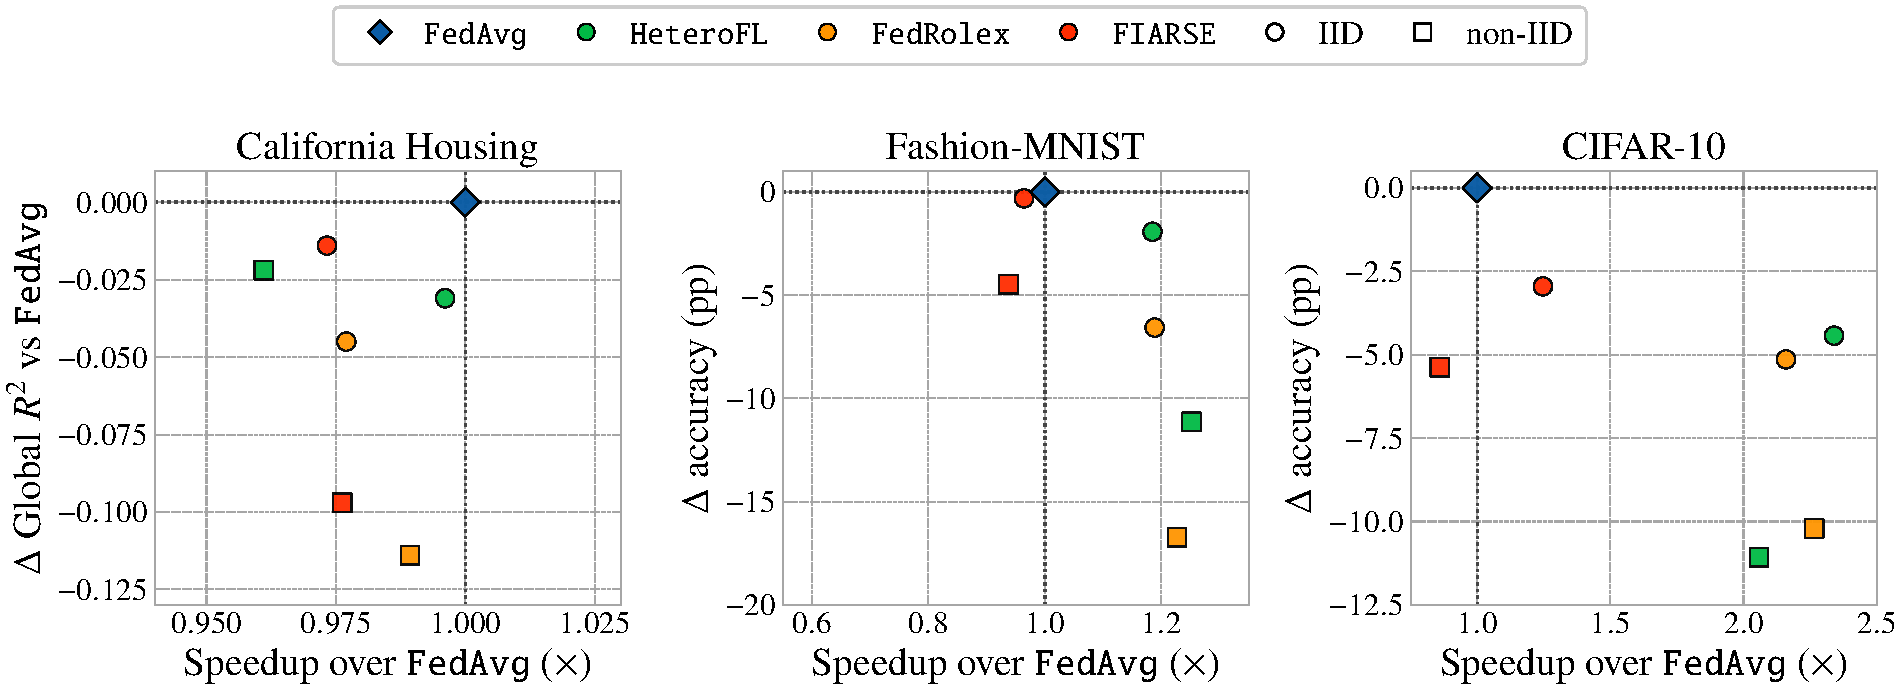
\includegraphics[width=0.95\textwidth]{figures/compute_main_quality_speed_tradeoff.pdf}
% Notes: points use mean global score and mean end-to-end runtime from Tables~\ref{tab:compute_main_results} and~\ref{tab:compute_main_runtime}.
% CIFAR-10 and Fashion-MNIST quality changes are percentage-point accuracy deltas; California Housing quality changes are raw R^2 deltas.
% The FedAvg diamond marks the reference point at 1x speedup and zero quality change in each task panel.
\caption{\textbf{Quality--speed trade-off relative to \texttt{FedAvg}.} Axes report wall-clock speedup and global-score change against the matching \texttt{FedAvg} baseline.}
% Non-baseline points compare a heterogeneous method against the matching \texttt{FedAvg} baseline for the same task and data regime; the \texttt{FedAvg} diamond marks the shared reference at \((1\times,0)\). The x-axis reports wall-clock speedup over \texttt{FedAvg}; the y-axis reports the change in global score, using \(R^2\) for California Housing and accuracy percentage points for CIFAR-10. Points to the right of \(1\times\) are faster than \texttt{FedAvg}, while points above zero improve global quality.}
\label{fig:compute_main_quality_speed_tradeoff}
\end{figure}

Figure~\ref{fig:compute_main_quality_speed_tradeoff} summarises the trade-off. California Housing stays near \(1\times\) speedup with lower quality. Fashion-MNIST shows moderate speedups for \texttt{HeteroFL} and \texttt{FedRolex}, but the quality loss is larger under non-IID data. CIFAR-10 separates the methods most strongly: \texttt{HeteroFL} and \texttt{FedRolex} give roughly \(2\times\) speedup, while \texttt{FIARSE} gives better submodel quality without realised wall-clock speedup on the dense-kernel execution path.



The client timing diagnostic in Figure~\ref{fig:compute_cifar10_client_train_time} shows why. \texttt{HeteroFL} and \texttt{FedRolex} keep the \texttt{rpi4} groups slower than \texttt{rpi5}, but the gap is moderate. \texttt{FIARSE} has much wider bands and higher \texttt{rpi4} training times, especially under non-IID sampling. This is an execution-level limitation: the current \texttt{FIARSE} path applies sparse masks inside dense PyTorch kernels rather than using sparse kernels or hardware-supported sparsity, so the algorithmic sparsity argument is not fully exercised by this wall-clock measurement \parencite{wu2024fiarse, hoefler2021sparsity}. Appendix~\ref{appendix:fashion_mnist_client_train_time} gives the corresponding Fashion-MNIST timing diagnostic.

\paragraph{Takeaways.}
\begin{itemize}[leftmargin=*, nosep]
  \item \texttt{FedAvg} remains the full-model quality control, reaching \(83.88\%\) IID Fashion-MNIST and \(79.38\%\) IID CIFAR-10 accuracy.
  \item \texttt{FIARSE} gives the strongest image-task quality profile among heterogeneous methods, including \(76.38\%\) non-IID Fashion-MNIST and \(70.55\%\) non-IID CIFAR-10 global accuracy.
  \item Runtime gains scale with local compute cost: \texttt{HeteroFL} and \texttt{FedRolex} give the clearest CIFAR-10 savings, while \texttt{FIARSE}'s sparse-mask quality benefit does not translate into wall-clock speedup on the dense PyTorch execution path.
\end{itemize}


\begin{figure}[H]
\centering
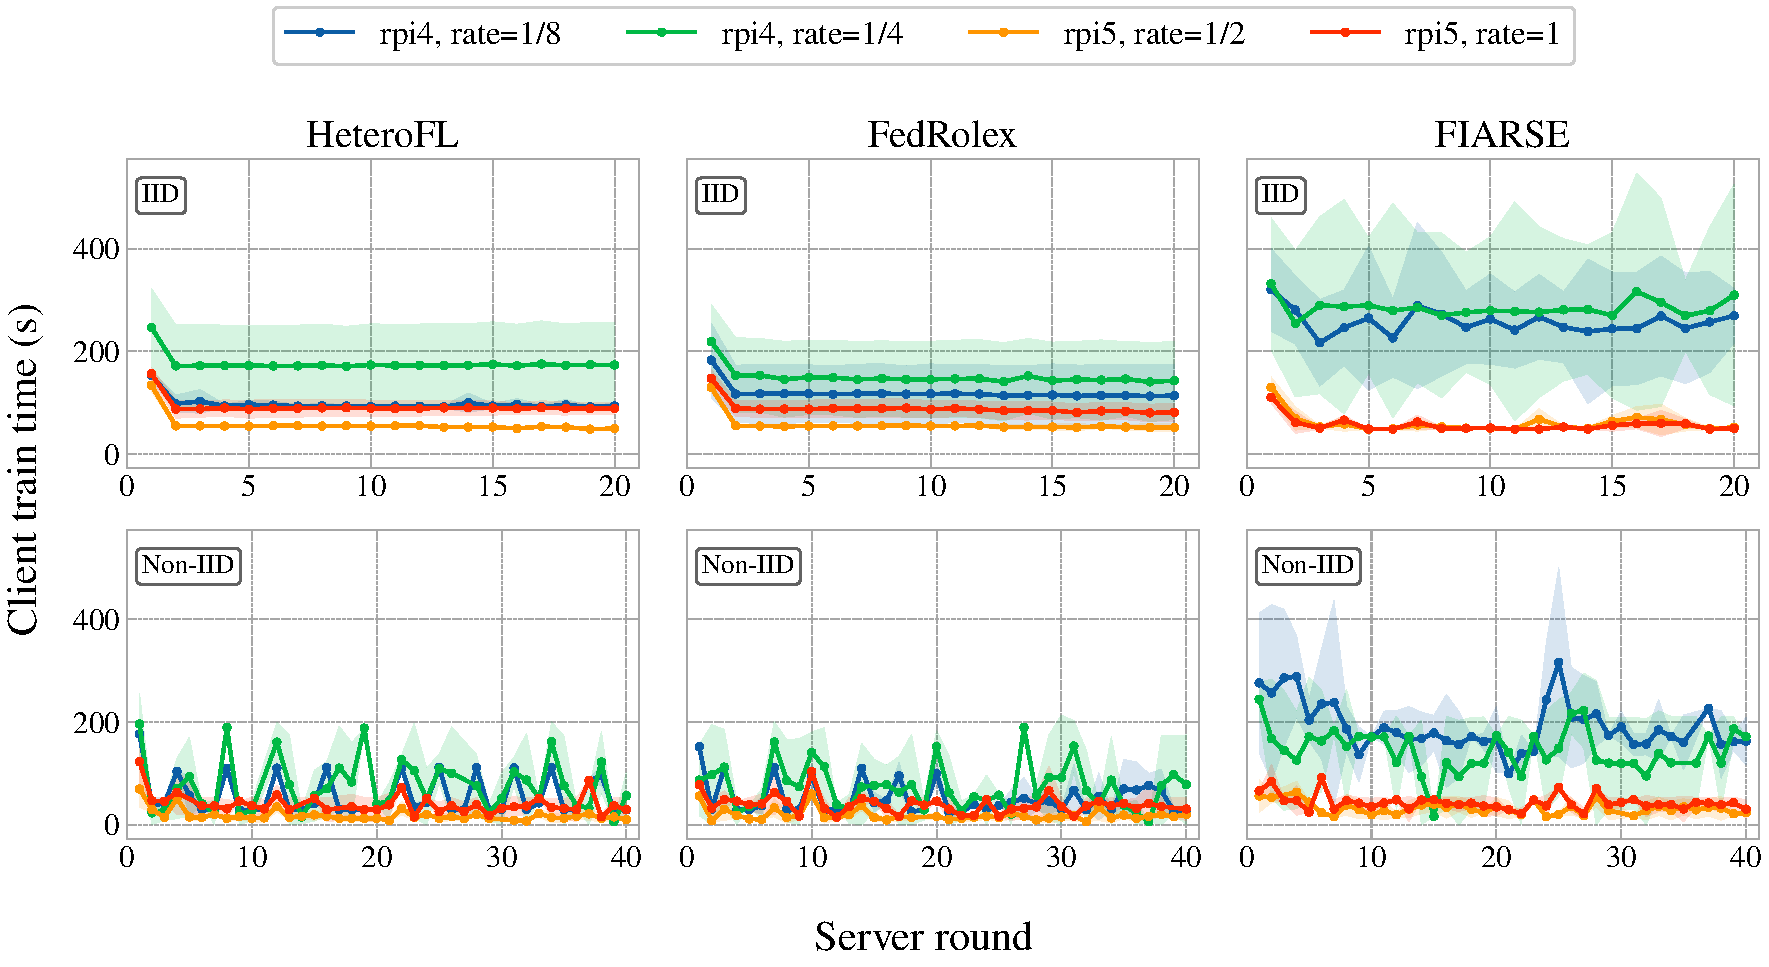
\includegraphics[width=0.98\textwidth]{figures/compute_main_cifar10_seed1340_client_train_time.pdf}
% Notes: rows are IID/non-IID and columns are HeteroFL, FedRolex, and FIARSE.
% Curves show mean update_train_duration_s for each device/rate group per server round.
% Shaded bands show within-group standard deviation across clients.
% IID reruns contain 20 rounds; non-IID reruns contain 40 rounds.
\caption{\textbf{Per-round client training time on CIFAR-10.} Curves split device/rate groups to show which clients gate synchronous rounds.}
\label{fig:compute_cifar10_client_train_time}
\end{figure}

\FloatBarrier
\subsection{Client-Side Submodel Quality}

\paragraph{Setup.}
This subsection addresses \evalqref{C3} by checking whether aggregate quality hides weak client-side submodels. To measure this, the final server model is converted into each rate-specific submodel, sent to every client, and evaluated on that client's local evaluation partition; the figures plot these per-client scores rather than centralized test scores. Figure~\ref{fig:compute_cifar10_seed1340_local_submodel_grid} reports the CIFAR-10 diagnostic, Figure~\ref{fig:compute_california_local_submodel_dist} reports the corresponding California Housing diagnostic, and Appendix~\ref{appendix:fashion_mnist_local_submodel_dist} gives the Fashion-MNIST counterpart.

\begin{figure}[!htbp]
\centering
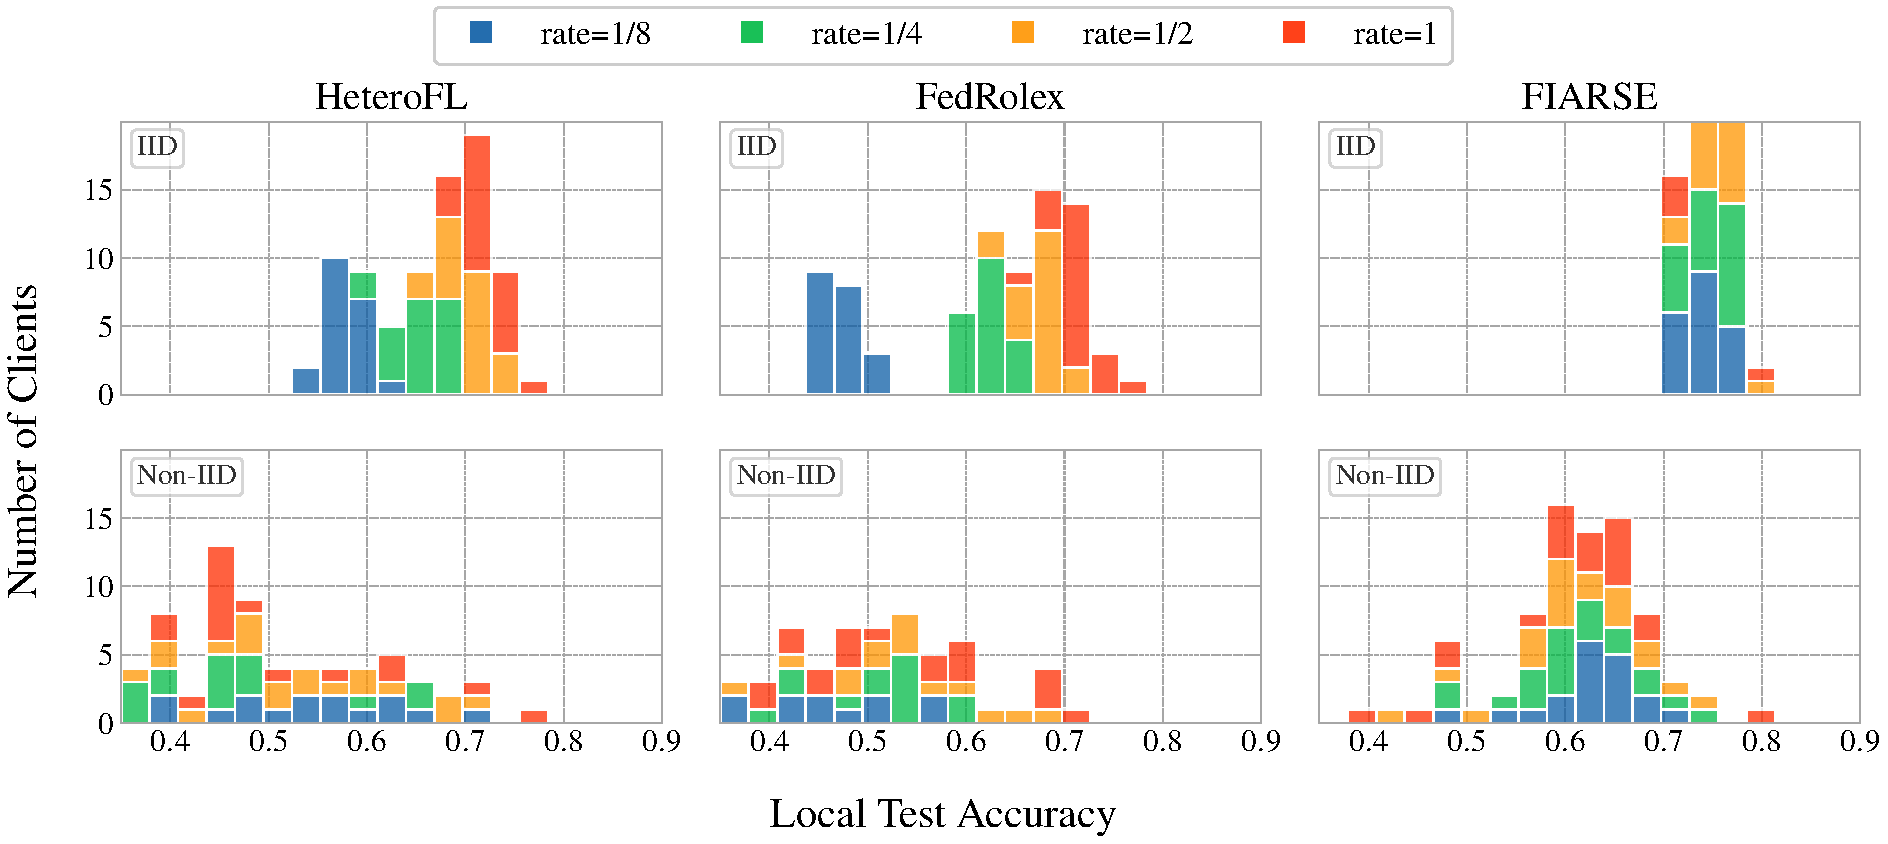
\includegraphics[width=0.98\textwidth]{figures/compute_main_cifar10_seed1340_local_submodel_grid.pdf}
% Notes: rows are IID/non-IID and columns are HeteroFL, FedRolex, and FIARSE.
% Each panel overlays final-round local test accuracy for rates 0.125, 0.25, 0.5, and 1.0 across 20 clients.
% Accuracy is measured on each client's local evaluation partition, not the global test set.
\caption{\textbf{Client-level CIFAR-10 local submodel accuracy distributions.}}
\label{fig:compute_cifar10_seed1340_local_submodel_grid}
\end{figure}

\paragraph{Interpretation.}
In IID CIFAR-10, \texttt{HeteroFL} and \texttt{FedRolex} show a clear rate-based performance gap: lower-rate submodels sit in lower accuracy bands than higher-rate submodels. This is a client-side fairness issue because weaker devices receive systematically weaker deployed models. \texttt{FIARSE} narrows this cross-rate spread, keeping low-rate and high-rate submodels closer together in a higher-accuracy band. Under non-IID data, \texttt{HeteroFL} and \texttt{FedRolex} become more dispersed and left-shifted; \texttt{FIARSE} remains more concentrated around \(60\)--\(70\%\).

\begin{figure}[!htbp]
\centering

\includegraphics[width=0.97\textwidth]{figures/compute_main_california_local_submodel_distributions.pdf}
% Notes: columns are HeteroFL, FedRolex, and FIARSE; rows are IID and non-IID.
% Each panel pools local-client tables from seeds 1337, 1338, and 1339 for that branch.
% The y-axis is clipped at -0.2 for readability; downward markers and annotations report clipped counts and minima.
\caption{\textbf{Client-level California Housing local submodel \(R^2\) distributions.} Panels pool local-client evaluations across seeds.}
\label{fig:compute_california_local_submodel_dist}
\end{figure}

The California Housing IID panels show similar ordering for \texttt{HeteroFL} and \texttt{FedRolex}; \texttt{FIARSE} is already strong at rate \(1/8\). Under non-IID partitioning, central performance remains usable for \texttt{HeteroFL} and \texttt{FIARSE}, but the lower tail becomes heavier and includes clipped negative outliers. \texttt{FedRolex} is especially weak at small rates. Aggregate accuracy and \(R^2\) therefore need to be read with client-level distributions.

\paragraph{Takeaways.}
\begin{itemize}[leftmargin=*, nosep]
  \item Aggregate scores are not enough for submodel FL because each weak client ultimately relies on a rate-specific submodel, not only the global network.
  \item \texttt{FIARSE} gives the most stable CIFAR-10 local-submodel distribution in the inspected reruns, especially under non-IID data.
  \item California Housing shows a residual robustness problem: even when central \(R^2\) is usable, some local submodels have poor tails.
\end{itemize}

\FloatBarrier
\subsection{Client-Capability Mix Sensitivity}

\paragraph{Setup.}
This subsection addresses \evalqref{C4}: whether the compute-heterogeneity result depends on the client-capability mix. The two-rate client-mix sweep varies the proportion of higher-capability clients from \(10\%\) to \(90\%\) while holding two model-rate levels at a time. The three columns in Figure~\ref{fig:compute_fixed_pair_triptych} compare rate \(1\) with rate \(1/4\), rate \(1\) with rate \(1/16\), and rate \(1/4\) with rate \(1/16\).


\paragraph{Interpretation.}
In the \(1\) vs \(1/4\) and \(1\) vs \(1/16\) columns, accuracy improves as the fraction of rate-\(1\) clients increases, but the curves flatten after the early mixture points. \texttt{FIARSE} is strongest when full-capacity clients are present, but dense-kernel execution keeps client training cost high and nearly flat. In the \(1/4\) vs \(1/16\) column, where no full-capacity clients are present, its accuracy advantage mostly disappears. \texttt{HeteroFL} and \texttt{FedRolex} therefore preserve the cleaner realised accuracy--time trade-off.


\begin{figure}[H]
\centering
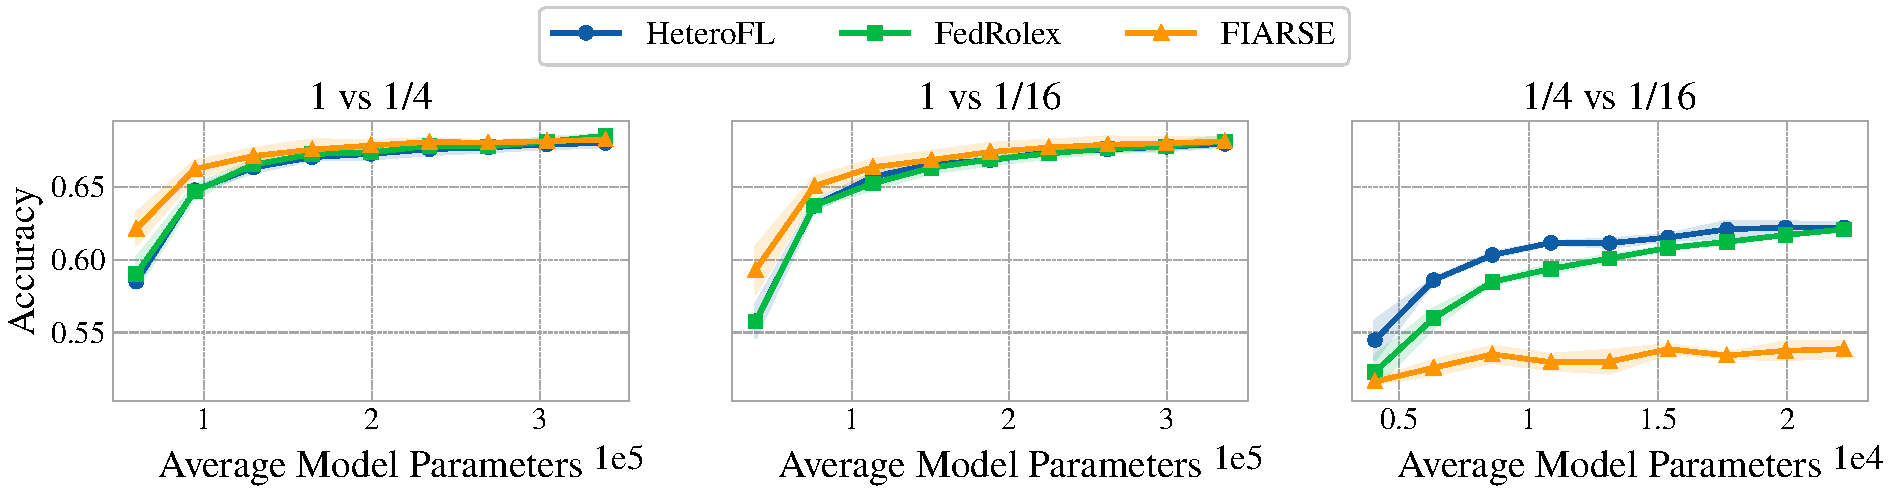
\includegraphics[width=\textwidth]{figures/fixed_pair_interpolation_triptych_methods.pdf}
% Notes: each column varies the proportion of higher-capability clients from 10% to 90%.
% Columns compare model-rate pairs 1 vs 1/4, 1 vs 1/16, and 1/4 vs 1/16.
% The top row reports final global accuracy against average client-side model parameters.
% Points aggregate seeds 1337--1339.
\caption{\textbf{Two-rate client-mix sweep on CIFAR-10 (IID).} Columns vary the client mix between two fixed model-rate levels.}
\label{fig:compute_fixed_pair_triptych}
\end{figure}



\paragraph{Takeaways.}
\begin{itemize}[leftmargin=*, nosep]
  \item The benefit of higher-capability clients is nonlinear: early capacity increases help most.
  \item \texttt{FIARSE}'s quality advantage depends on access to full-capacity clients; sparse-kernel support remains a separate requirement for testing its intended CIFAR-10 runtime benefit.
  \item When only reduced-rate clients are present, \texttt{HeteroFL} and \texttt{FedRolex} give the cleaner realised accuracy--time trade-off.
\end{itemize}

\FloatBarrier
\section{Straggler-Induced Heterogeneity}
\label{sec:eval_network_heterogeneity}

Straggler-induced heterogeneity changes when updates arrive, how stale they are when applied, and how often slower devices influence the server model, as introduced in Section~\ref{sec:background_straggler_heterogeneity}. Previous asynchronous-FL evaluations often simulate staleness or client delay; the cluster runs here measure completion time, staleness, update share, and aggregate weight share directly. The corresponding method family is asynchronous FL, reviewed in Section~\ref{sec:related_async_fl}. This section evaluates asynchronous FL before Section~\ref{sec:eval_async_submodel_fl} combines it with submodel training.

\FloatBarrier
\subsection{Asynchronous FL Across Data and Device Heterogeneity}

\paragraph{Setup.}
This subsection addresses \evalqref{S1}: how asynchronous FL behaves across data regimes and device placements. The CIFAR-10 benchmark crosses \texttt{IID} versus \texttt{non-IID} data with two placements: a homogeneous all-\texttt{rpi5} baseline and a mixed \texttt{rpi4}/\texttt{rpi5} straggler setting. Since all clients train the same model capacity, the placement contrast reflects straggler-induced timing rather than submodel-capacity effects. The methods are \texttt{FedAvg}, \texttt{FedAsync}, \texttt{FedBuff}, and \texttt{FedStaleWeight}, abbreviated as \texttt{FedSW} in compact tables and figures; Appendix~\ref{appendix:evaluation_settings}, Table~\ref{tab:appendix_straggler_settings}, lists their run budgets, buffer sizes, and concurrency settings.

The endpoint is the first server evaluation reaching \(60\%\) accuracy. Time-to-target reports elapsed wall-clock time, while trips to target counts completed client updates to the same threshold; slow-device update share and aggregate-weight share diagnose representation. Figure~\ref{fig:network_main_setup_matrix} summarises the setup and shared stopping rule. Reporting both time and trips separates faster update arrival from better data efficiency, which matters when deployed FL methods are chosen for usable models under a wall-clock budget.

% The mixed-topology rows are completed reruns under the intended placement; earlier submissions had inherited the packed all-\texttt{rpi5} deploy config.

\begin{figure}[!htbp]
\centering
\makebox[\textwidth][c]{%
\hspace*{-0.25cm}%
\begin{tikzpicture}[
  font=\small,
  cell/.style={draw=black!25, rounded corners=2pt, fill=black!3, minimum width=4.35cm, minimum height=1.55cm, align=center},
  header/.style={font=\footnotesize\bfseries, align=center, text=black!75},
  rowlab/.style={font=\footnotesize\bfseries, align=right, text=black!75},
  note/.style={font=\scriptsize, align=center, text=black!70},
  infobox/.style={draw=black!25, rounded corners=2pt, fill=white, minimum width=3.95cm, minimum height=0.8cm, text width=3.55cm, align=center},
  targetbox/.style={draw=paletteGreen!55!black, rounded corners=2pt, fill=paletteGreen!9, minimum width=3.95cm, minimum height=1.0cm, text width=3.55cm, align=center},
  dotrpi5/.style={circle, draw=paletteGreen!80!black, fill=paletteGreen!20, minimum size=4.8mm, inner sep=0pt},
  dotrpi4/.style={circle, draw=paletteOrange!90!black, fill=paletteOrange!22, minimum size=4.8mm, inner sep=0pt},
  arrow/.style={-Latex, line width=0.5pt, draw=black!48}
]
\node[header] at (2.55,4.25) {Control topology\\packed all-\texttt{rpi5}};
\node[header] at (7.25,4.25) {Treatment topology\\mixed \texttt{rpi5}/\texttt{rpi4}};
\node[header, align=left] at (12.05,4.25) {Common run budget\\and endpoint};

\node[cell] (iid5) at (2.55,2.75) {};
\node[cell] (iidm) at (7.25,2.75) {};
\node[cell] (non5) at (2.55,0.45) {};
\node[cell] (nonm) at (7.25,0.45) {};
\node[rowlab] at (-0.3,2.75) {\texttt{IID}\\data};
\node[rowlab] at (-0.4,0.45) {\texttt{non-IID}\\data};

\foreach \n in {iid5,non5} {
  \node[dotrpi5] at ($(\n.center)+(-0.55,0.30)$) {};
  \node[note, text=paletteGreen!70!black] at ($(\n.center)+(0.35,0.30)$) {\(15\times\texttt{rpi5}\)};
  \node[note, text width=3.55cm] at ($(\n.center)+(0,-0.42)$) {homogeneous timing};
}
\foreach \n in {iidm,nonm} {
  \node[dotrpi5] at ($(\n.center)+(-0.70,0.36)$) {};
  \node[note, text=paletteGreen!70!black] at ($(\n.center)+(0.16,0.36)$) {\(10\times\texttt{rpi5}\)};
  \node[dotrpi4] at ($(\n.center)+(-0.70,-0.06)$) {};
  \node[note, text=paletteOrange!90!black] at ($(\n.center)+(0.16,-0.06)$) {\(5\times\texttt{rpi4}\)};
  \node[note, text width=3.55cm] at ($(\n.center)+(0,-0.55)$) {straggler-prone timing};
}

\node[note, infobox]
  (methods) at (12.05,2.75)
  {\texttt{FedAvg}: \(50\) rounds\\
   asynchronous methods: \(100\) server steps};
\node[note, targetbox]
  (target) at (12.05,0.45)
  {first \(60\%\) CIFAR-10 validation accuracy\\
   reported as client trips and wall-clock time};

\draw[arrow] (iidm.east) -- (methods.west);
\draw[arrow] (nonm.east) -- (target.west);
\draw[arrow] (methods.south) -- (target.north);
\end{tikzpicture}%
}
\caption{\textbf{Straggler-induced heterogeneity setup.} Data regime is crossed with topology; the mixed column is the slow-client treatment.}
\label{fig:network_main_setup_matrix}
\end{figure}

% The representation diagnostic is the \texttt{rpi4} update and aggregate-weight share relative to its \(33.3\%\) population share.


\begin{table}[H]
\centering
\scriptsize
% Notes: no-impairment 2x2 matrix over data regime and topology; entries are mean +/- standard deviation over seeds 1337--1339.
% Target-attainment columns report the first point reaching 60% validation accuracy in client trips, wall-clock seconds, and derived throughput.
% Lower is better for trips/time; highlighted target-attainment cells rank the asynchronous methods within each setting.
% Daggered target-attainment cells are lower-bound aggregates: one or more seeds did not reach target, so the final observed client trips or wall-clock time was substituted.
% Diagnostics report accepted-update share, normalized aggregate weight share, and mean staleness in server steps; staleness and throughput cells report means only.
% Daggered values are structural baselines inferred from topology rather than measured asynchronous summaries.
\caption{\textbf{Straggler-induced heterogeneity target-attainment and diagnostics on CIFAR-10.} Columns report trips/time to \(60\%\), update and weight share, and staleness.}
\label{tab:network_main_target_matrix}

\setlength{\tabcolsep}{2.2pt}
\begin{adjustbox}{max width=\textwidth}
\begin{tabular}{@{}lllcccccc@{}}
\toprule
& & & \multicolumn{3}{c}{Target attainment} & \multicolumn{3}{c}{Diagnostics} \\
\cmidrule(lr){4-6}\cmidrule(l){7-9}
Data & Topology & Method
& \makecell{Trips\\to target}
& \makecell{Time to\\target (s)}
& \makecell{Trips/s\\to target}
& \makecell{\texttt{rpi4}\\update \%}
& \makecell{\texttt{rpi4}\\weight \%}
& \makecell{Staleness\\\texttt{rpi4}/\texttt{rpi5}} \\
\midrule
\multirow{8}{*}{IID}
 & \multirow{4}{*}{all-\texttt{rpi5}} & \texttt{FedAvg} & \(195 \pm 0\) & \(651 \pm 34\) & \(0.300\) & \(0.0^\dagger\) & \(0.0^\dagger\) & -- / \(0^\dagger\) \\
 & & \texttt{FedAsync} & \evalbest{\(257 \pm 12\)} & \evalsecond{\(722 \pm 29\)} & \(0.355\) & \(0.0^\dagger\) & \(0.0^\dagger\) & -- / \(13.54\) \\
 & & \texttt{FedBuff} & \(343 \pm 90\) & \(880 \pm 210\) & \(0.390\) & \(0.0^\dagger\) & \(0.0^\dagger\) & -- / \(1.34\) \\
 & & \texttt{FedSW} & \evalsecond{\(273 \pm 6\)} & \evalbest{\(715 \pm 4\)} & \(0.382\) & \(0.0^\dagger\) & \(0.0^\dagger\) & -- / \(1.33\) \\
\cmidrule(lr){2-9}
 & \multirow{4}{*}{mixed} & \texttt{FedAvg} & \(195 \pm 0\) & \(2097 \pm 5\) & \(0.093\) & \(33.3^\dagger\) & \(33.3^\dagger\) & \(0^\dagger\) / \(0^\dagger\) \\
 & & \texttt{FedAsync} & \evalbest{\(137 \pm 6\)} & \evalbest{\(622 \pm 9\)} & \(0.220\) & \(11.9 \pm 0.8\) & \(6.7 \pm 0.7\) & \(35.68\) / \(9.90\) \\
 & & \texttt{FedBuff} & \(387 \pm 15\) & \(1138 \pm 77\) & \(0.340\) & \(13.8 \pm 0.6\) & \(10.1 \pm 0.7\) & \(3.23\) / \(1.05\) \\
 & & \texttt{FedSW} & \evalsecond{\(280 \pm 0\)} & \evalsecond{\(865 \pm 31\)} & \(0.324\) & \(13.8 \pm 0.8\) & \(27.9 \pm 0.7\) & \(3.16\) / \(1.03\) \\
\midrule
\multirow{8}{*}{Non-IID}
 & \multirow{4}{*}{all-\texttt{rpi5}} & \texttt{FedAvg} & \(425 \pm 69\) & \(1320 \pm 205\) & \(0.322\) & \(0.0^\dagger\) & \(0.0^\dagger\) & -- / \(0^\dagger\) \\
 & & \texttt{FedAsync} & \evalsecond{\evalcensored{953 \pm 57}} & \evalcensored{2394 \pm 127} & \(0.398\) & \(0.0^\dagger\) & \(0.0^\dagger\) & -- / \(13.88\) \\
 & & \texttt{FedBuff} & \evalcensored{973 \pm 46} & \evalsecond{\evalcensored{2293 \pm 109}} & \(0.424\) & \(0.0^\dagger\) & \(0.0^\dagger\) & -- / \(1.38\) \\
 & & \texttt{FedSW} & \evalbest{\(620 \pm 85\)} & \evalbest{\(1486 \pm 181\)} & \(0.417\) & \(0.0^\dagger\) & \(0.0^\dagger\) & -- / \(1.37\) \\
\cmidrule(lr){2-9}
 & \multirow{4}{*}{mixed} & \texttt{FedAvg} & \(420 \pm 78\) & \(4043 \pm 437\) & \(0.104\) & \(33.3^\dagger\) & \(33.3^\dagger\) & \(0^\dagger\) / \(0^\dagger\) \\
 & & \texttt{FedAsync} & \evalbest{\(390 \pm 44\)} & \evalbest{\(1264 \pm 111\)} & \(0.309\) & \(12.9 \pm 0.7\) & \(7.5 \pm 0.7\) & \(35.99\) / \(10.33\) \\
 & & \texttt{FedBuff} & \(913 \pm 84\) & \(2388 \pm 128\) & \(0.382\) & \(14.6 \pm 0.7\) & \(10.7 \pm 0.6\) & \(3.27\) / \(1.05\) \\
 & & \texttt{FedSW} & \evalsecond{\(633 \pm 55\)} & \evalsecond{\(1771 \pm 132\)} & \(0.357\) & \(14.6 \pm 0.6\) & \(29.7 \pm 0.3\) & \(3.17\) / \(1.06\) \\
\bottomrule
\end{tabular}
\end{adjustbox}
\par\vspace{0.2em}
{\centering\scriptsize \(\ddagger\) lower-bound aggregate: at least one seed did not reach target.\\\textcolor{evalBestText}{\textbf{Red bold}} text marks the \textbf{best} value and \textcolor{evalSecondText}{blue} text the \textbf{second-best} value among comparable entries. \par}
\end{table}

% \par\vspace{0.5em}
% {\centering\scriptsize \textcolor{evalBestText}{\textbf{Red bold}} text marks the \textbf{best} value and \textcolor{evalSecondText}{blue} text the \textbf{second-best} value among comparable entries.\par}

\paragraph{Interpretation.}
The all-\texttt{rpi5} rows are the negative control: \texttt{FedAvg} reaches the target first in both IID and non-IID settings, while some asynchronous non-IID seeds do not reach target within the trip budget. Mixed topology reverses the wall-clock result. In IID mixed runs, \texttt{FedAsync} reaches target in \(137\pm6\) client trips and \(622\pm9\) s, compared with \(195\pm0\) trips and \(2097\pm5\) s for \texttt{FedAvg}; it is also fastest in non-IID mixed runs. Asynchrony therefore helps under mixed completion times, not simply under non-IID data.


Figure~\ref{fig:network_main_accuracy_combined} shows that asynchronous methods are not consistently more data-efficient. In the all-\texttt{rpi5} panels, \texttt{FedAvg} reaches \(60\%\) with fewer completed trips. The deployment advantage appears only in the wall-clock row: the mixed \texttt{FedAvg} curves are stretched far to the right because synchronous rounds wait for slow devices. \texttt{FedAsync} is fastest, but its speed has a representation cost: \texttt{rpi4} clients provide only about \(12\)--\(13\%\) of accepted updates and roughly \(7\%\) of aggregate weight. \texttt{FedStaleWeight} is slower but raises \texttt{rpi4} aggregate weight to roughly \(28\)--\(30\%\), much closer to the \(5/15\) population share.



\begin{figure}[H]
\centering
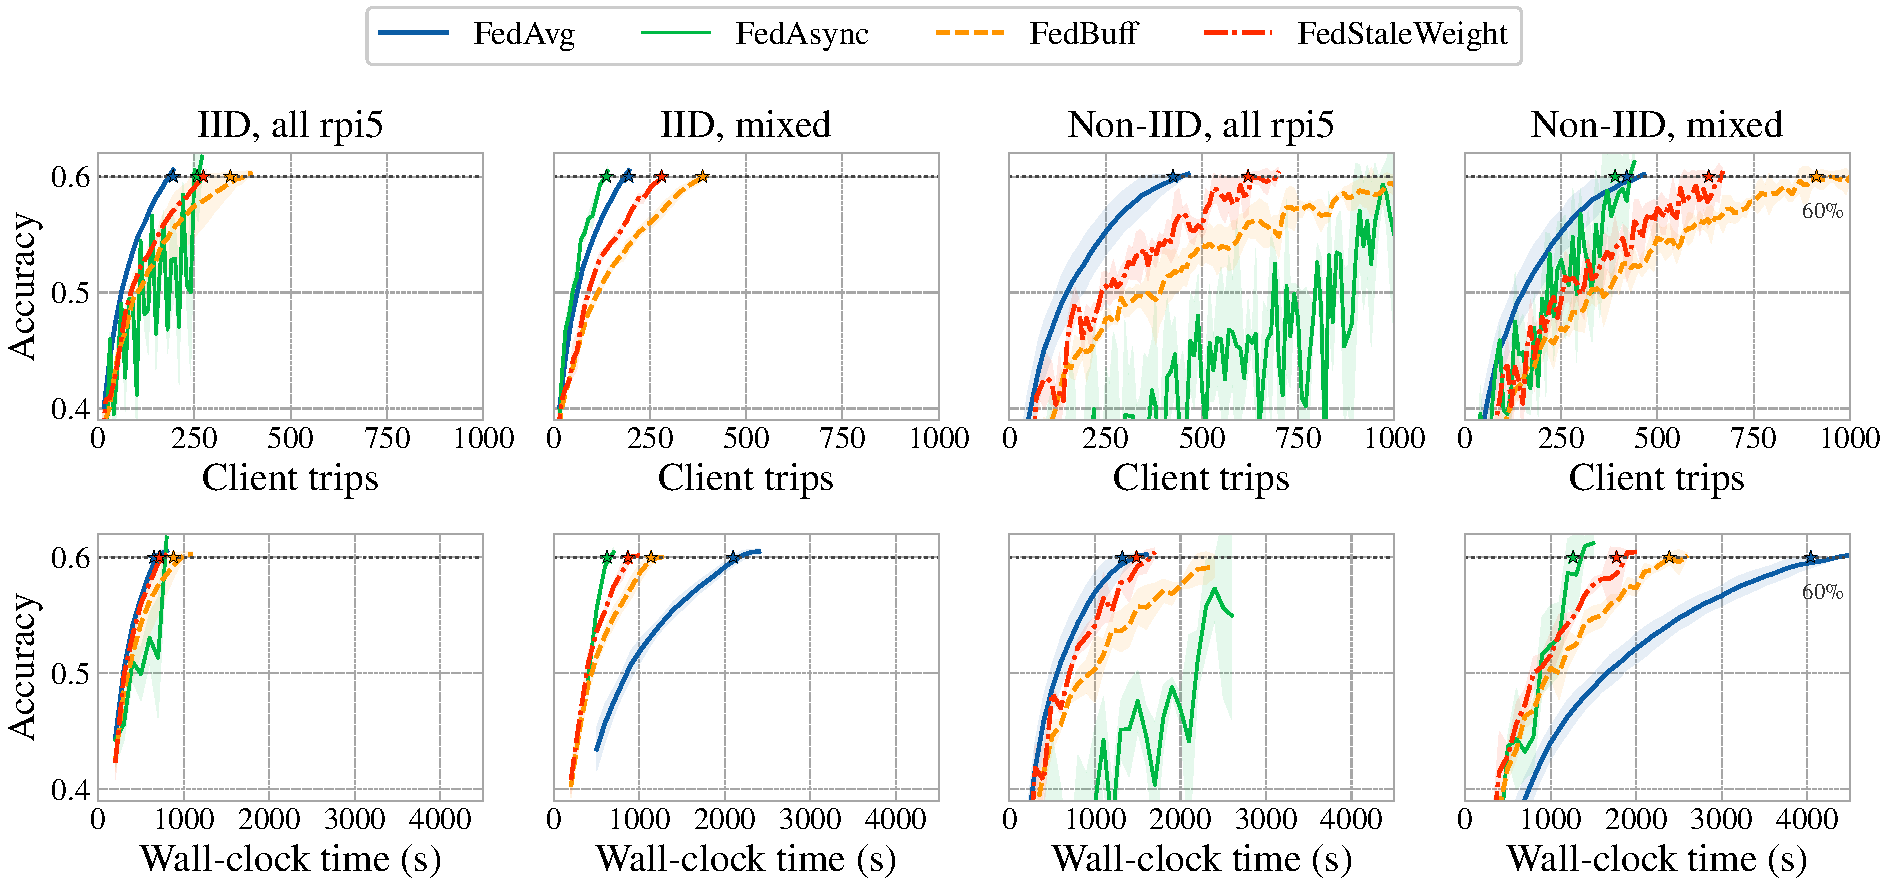
\includegraphics[width=\textwidth]{figures/network_main_accuracy_combined.pdf}
% Notes: top row plots completed client trips; bottom row plots elapsed wall-clock time. Curves show three-seed means with +/- one-standard-deviation bands; the dotted line marks the 60% target.
\caption{\textbf{Straggler-induced heterogeneity accuracy by completed client trips and elapsed wall-clock time.} The dotted horizontal line marks the \(60\%\) target.}
\label{fig:network_main_accuracy_combined}
\end{figure}


\paragraph{Takeaways.}
\begin{itemize}[leftmargin=*, nosep]
  \item In homogeneous all-\texttt{rpi5} runs, synchrony is the better control: \texttt{FedAvg} reaches the target with fewer client trips.
  \item In mixed topology, \texttt{FedAsync} is the fastest wall-clock method, reaching target in \(622\pm9\) s for IID and \(1264\pm111\) s for non-IID.
  \item The speed gain carries a representation cost, while \texttt{FedStaleWeight} trades speed for \texttt{rpi4} aggregate weight closer to population share.
\end{itemize}

\FloatBarrier
\subsection{Network Perturbations: Speed and Representation}

\paragraph{Setup.}
This subsection addresses \evalqref{S2}: how network perturbations affect asynchronous speed and slow-device representation when completion times are mixed. The no-impairment profile is the control; the \texttt{netem} profiles add delay, jitter, loss, and asymmetric bandwidth limits without changing the run config. The experiment also adds \(K=5\) variants for \texttt{FedBuff} and \texttt{FedStaleWeight}, reported in Table~\ref{tab:network_stressor_sweep} as \texttt{FedBuff}\(_5\) and \texttt{FedSW}\(_5\); the main buffered runs use \(K=10\). Smaller buffers test whether buffer-fill latency or update diversity dominates target time under these perturbations.


\begin{figure}[!htbp]
\centering
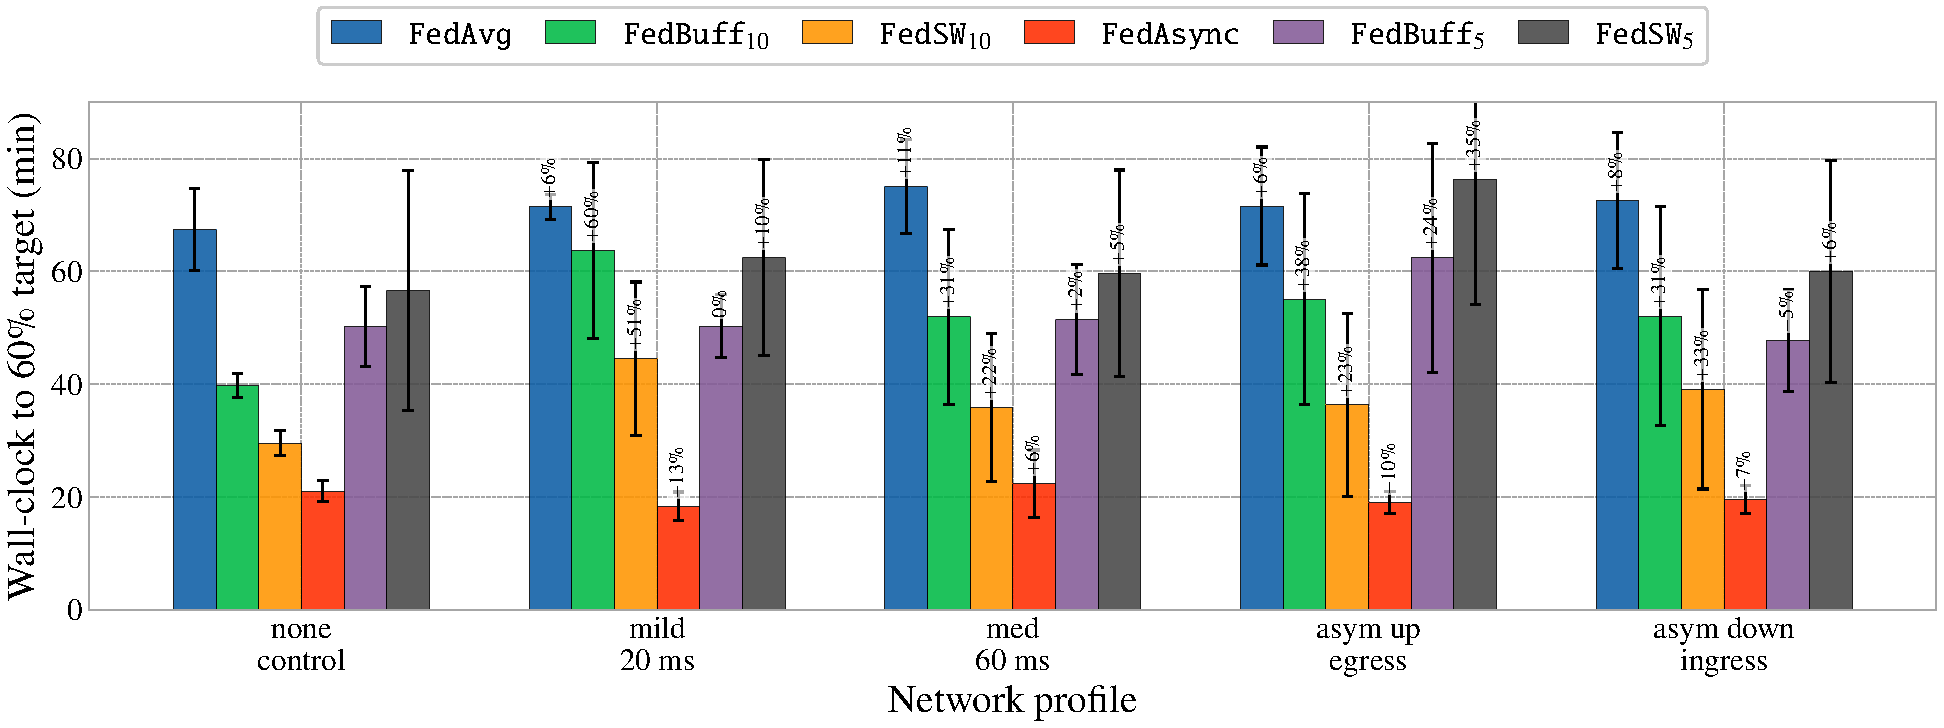
\includegraphics[width=\textwidth]{figures/network_stressor_profile_bars.pdf}
% Notes: bars aggregate seeds 1337--1339. Labels above stressed-profile bars show percentage change from the same method under no added impairment. When a seed did not reach target, its final observed wall-clock time is substituted in the aggregate.
\caption{\textbf{Wall-clock target time across network-stressor profiles.} Labels above stressed-profile bars show percentage change compared to the no-impairment baseline.}
\label{fig:network_stressor_profile_bars}
\end{figure}



\begin{table}[!htbp]
\centering
\scriptsize
% Notes: all runs use 10 rpi5 + 5 rpi4, full local models, and a 60% target.
% Values aggregate seeds 1337, 1338, and 1339.
% The none rows for FedAvg, FedBuff_10, FedSW_10, and FedAsync reuse corresponding main straggler-induced heterogeneity mixed non-IID runs.
% Other rows come from the network_stressor_sweep W&B group.
% Daggered target-attainment cells are lower-bound aggregates: one or more seeds did not reach target, so the final observed client trips or wall-clock time was substituted.
% Diagnostic columns are shown only for asynchronous runs.
\caption{\textbf{Network-stressor sweep on non-IID CIFAR-10 mixed topology.} Rows compare no-impairment and \texttt{netem} profiles, with \(K=10\) and \(K=5\) buffered runs.}
\label{tab:network_stressor_sweep}
\setlength{\tabcolsep}{2.2pt}
\begin{adjustbox}{max width=\textwidth}
\begin{tabular}{@{}p{3.5cm}lrrrrrrr@{}}
\toprule
& & \multicolumn{3}{c}{Target attainment} & \multicolumn{4}{c}{Diagnostics} \\
\cmidrule(lr){3-5}\cmidrule(l){6-9}
\makecell{Profile  /\\Impairment} & Method
& \makecell{Trips\\to target}
& \makecell{Time to\\target (s)}
& \makecell{Final\\acc.}
& \makecell{\texttt{rpi4}\\update \%}
& \makecell{\texttt{rpi4}\\weight \%}
& \makecell{Staleness\\\texttt{rpi4}/\texttt{rpi5}}
& \makecell{Updates/s} \\
\midrule
\multirow{6}{=}{\centering \texttt{none}\\[0.25em]No added impairment}
 & \texttt{FedAvg} & \(420 \pm 78\) & \(4043 \pm 437\) & \(60.2 \pm 0.2\) & -- & -- & -- / -- & -- \\
 & \texttt{FedBuff}\(_{10}\) & \(913 \pm 84\) & \(2388 \pm 128\) & \(60.1 \pm 0.2\) & \(14.6 \pm 0.7\) & \(10.7 \pm 0.6\) & \(3.27\) / \(1.05\) & \(0.382\) \\
 & \texttt{FedSW}\(_{10}\) & \(633 \pm 55\) & \evalsecond{\(1771 \pm 132\)} & \(60.5 \pm 0.2\) & \(14.6 \pm 0.6\) & \(29.7 \pm 0.3\) & \(3.17\) / \(1.06\) & \(0.357\) \\
 & \texttt{FedAsync} & \evalbest{\(390 \pm 44\)} & \evalbest{\(1264 \pm 111\)} & \(61.2 \pm 1.3\) & \(12.9 \pm 0.7\) & \(7.5 \pm 0.7\) & \(35.99\) / \(10.33\) & \(0.308\) \\
 & \texttt{FedBuff}\(_{5}\) & \evalsecond{\(587 \pm 50\)} & \(3014 \pm 423\) & \(60.6 \pm 0.3\) & \(21.4 \pm 1.4\) & \(17.6 \pm 1.7\) & \(4.38\) / \(2.31\) & \(0.198\) \\
 & \texttt{FedSW}\(_{5}\) & \evalcensored{645 \pm 130} & \evalcensored{3396 \pm 1277} & \(53.9 \pm 11.8\) & \(20.5 \pm 1.8\) & \(30.0 \pm 1.1\) & \(4.58\) / \(2.28\) & \(0.199\) \\
\midrule
\multirow{6}{=}{\centering \texttt{mild}\\[0.25em]20 ms, 5 ms jitter\\100 Mbit/s}
 & \texttt{FedAvg} & \(425 \pm 69\) & \(4286 \pm 136\) & \(60.2 \pm 0.1\) & -- & -- & -- / -- & -- \\
 & \texttt{FedBuff}\(_{10}\) & \(900 \pm 104\) & \(3825 \pm 936\) & \(60.4 \pm 0.4\) & \(19.0 \pm 3.4\) & \(15.6 \pm 3.7\) & \(2.54\) / \(1.12\) & \(0.252\) \\
 & \texttt{FedSW}\(_{10}\) & \(617 \pm 40\) & \evalsecond{\(2672 \pm 815\)} & \(60.4 \pm 0.3\) & \(18.9 \pm 4.0\) & \(31.7 \pm 0.7\) & \(2.59\) / \(1.11\) & \(0.253\) \\
 & \texttt{FedAsync} & \evalbest{\(360 \pm 56\)} & \evalbest{\(1101 \pm 152\)} & \(62.2 \pm 1.9\) & \(13.7 \pm 0.7\) & \(8.3 \pm 0.8\) & \(33.49\) / \(10.41\) & \(0.326\) \\
 & \texttt{FedBuff}\(_{5}\) & \evalsecond{\(595 \pm 65\)} & \(3018 \pm 336\) & \(60.3 \pm 0.2\) & \(20.8 \pm 1.9\) & \(17.0 \pm 2.1\) & \(4.47\) / \(2.30\) & \(0.200\) \\
 & \texttt{FedSW}\(_{5}\) & \evalcensored{717 \pm 58} & \evalcensored{3746 \pm 1040} & \(53.5 \pm 8.9\) & \(21.1 \pm 2.4\) & \(30.3 \pm 1.2\) & \(4.48\) / \(2.31\) & \(0.199\) \\
\midrule
\multirow{6}{=}{\centering \texttt{med}\\[0.25em]60 ms, 15 ms jitter\\0.5\% loss, 50 Mbit/s}
 & \texttt{FedAvg} & \(425 \pm 69\) & \(4500 \pm 498\) & \(60.2 \pm 0.1\) & -- & -- & -- / -- & -- \\
 & \texttt{FedBuff}\(_{10}\) & \(923 \pm 121\) & \(3119 \pm 930\) & \(60.4 \pm 0.4\) & \(16.2 \pm 4.1\) & \(12.6 \pm 4.4\) & \(3.05\) / \(1.08\) & \(0.317\) \\
 & \texttt{FedSW}\(_{10}\) & \(620 \pm 69\) & \evalsecond{\(2155 \pm 787\)} & \(60.5 \pm 0.4\) & \(16.3 \pm 4.1\) & \(30.9 \pm 1.0\) & \(3.00\) / \(1.07\) & \(0.313\) \\
 & \texttt{FedAsync} & \evalbest{\(360 \pm 20\)} & \evalbest{\(1341 \pm 359\)} & \(61.0 \pm 0.9\) & \(13.6 \pm 1.2\) & \(8.2 \pm 1.2\) & \(33.96\) / \(10.39\) & \(0.280\) \\
 & \texttt{FedBuff}\(_{5}\) & \evalsecond{\(603 \pm 28\)} & \(3084 \pm 584\) & \(60.4 \pm 0.4\) & \(20.8 \pm 2.1\) & \(17.1 \pm 2.3\) & \(4.49\) / \(2.30\) & \(0.201\) \\
 & \texttt{FedSW}\(_{5}\) & \evalcensored{692 \pm 101} & \evalcensored{3582 \pm 1097} & \(53.2 \pm 7.9\) & \(20.8 \pm 2.3\) & \(29.8 \pm 1.6\) & \(4.52\) / \(2.30\) & \(0.201\) \\
\midrule
\multirow{6}{=}{\centering \makecell[c]{\texttt{asym up}}\\[0.25em]Egress only\\90 ms, 20 ms jitter\\0.5\% loss, 20 Mbit/s}
 & \texttt{FedAvg} & \(420 \pm 65\) & \(4295 \pm 627\) & \(60.1 \pm 0.1\) & -- & -- & -- / -- & -- \\
 & \texttt{FedBuff}\(_{10}\) & \(960 \pm 92\) & \(3306 \pm 1123\) & \(60.2 \pm 0.1\) & \(16.2 \pm 4.2\) & \(12.5 \pm 4.5\) & \(3.04\) / \(1.08\) & \(0.314\) \\
 & \texttt{FedSW}\(_{10}\) & \(617 \pm 55\) & \evalsecond{\(2179 \pm 973\)} & \(60.1 \pm 0.1\) & \(16.0 \pm 4.2\) & \(31.0 \pm 1.5\) & \(3.09\) / \(1.07\) & \(0.315\) \\
 & \texttt{FedAsync} & \evalbest{\(380 \pm 44\)} & \evalbest{\(1141 \pm 115\)} & \(61.2 \pm 1.5\) & \(13.6 \pm 0.8\) & \(8.2 \pm 0.9\) & \(33.88\) / \(10.42\) & \(0.333\) \\
 & \texttt{FedBuff}\(_{5}\) & \evalsecond{\(582 \pm 72\)} & \(3745 \pm 1218\) & \(60.4 \pm 0.3\) & \(21.6 \pm 1.2\) & \(17.8 \pm 1.4\) & \(4.38\) / \(2.30\) & \(0.165\) \\
 & \texttt{FedSW}\(_{5}\) & \evalcensored{735 \pm 26} & \evalcensored{4580 \pm 1329} & \(46.5 \pm 12.2\) & \(21.3 \pm 1.3\) & \(30.6 \pm 0.4\) & \(4.41\) / \(2.32\) & \(0.170\) \\
\midrule
\multirow{6}{=}{\centering \makecell[c]{\texttt{asym down}}\\[0.25em]Ingress only\\90 ms, 20 ms jitter\\0.5\% loss, 20 Mbit/s}
 & \texttt{FedAvg} & \(425 \pm 69\) & \(4351 \pm 722\) & \(60.2 \pm 0.1\) & -- & -- & -- / -- & -- \\
 & \texttt{FedBuff}\(_{10}\) & \(913 \pm 67\) & \(3125 \pm 1163\) & \(60.4 \pm 0.3\) & \(16.6 \pm 4.0\) & \(13.0 \pm 4.2\) & \(2.96\) / \(1.08\) & \(0.319\) \\
 & \texttt{FedSW}\(_{10}\) & \(667 \pm 23\) & \evalsecond{\(2348 \pm 1062\)} & \(60.4 \pm 0.5\) & \(16.5 \pm 4.0\) & \(31.0 \pm 1.0\) & \(2.99\) / \(1.07\) & \(0.317\) \\
 & \texttt{FedAsync} & \evalbest{\(393 \pm 57\)} & \evalbest{\(1173 \pm 152\)} & \(61.9 \pm 2.0\) & \(13.3 \pm 0.5\) & \(8.0 \pm 0.7\) & \(34.56\) / \(10.38\) & \(0.335\) \\
 & \texttt{FedBuff}\(_{5}\) & \evalsecond{\(555 \pm 78\)} & \(2867 \pm 543\) & \(60.4 \pm 0.3\) & \(20.7 \pm 2.0\) & \(16.9 \pm 2.2\) & \(4.51\) / \(2.29\) & \(0.198\) \\
 & \texttt{FedSW}\(_{5}\) & \evalcensored{693 \pm 98} & \evalcensored{3600 \pm 1178} & \(54.8 \pm 6.2\) & \(21.0 \pm 1.7\) & \(30.2 \pm 0.9\) & \(4.51\) / \(2.30\) & \(0.202\) \\
\bottomrule
\end{tabular}
\end{adjustbox}
\par\vspace{0.2em}
{\centering\scriptsize \(\ddagger\) lower-bound aggregate: at least one seed did not reach target. \\ \textcolor{evalBestText}{\textbf{Red bold}} text marks the \textbf{best} value and \textcolor{evalSecondText}{blue} text the \textbf{second-best} value among comparable entries. \par}

\end{table}

\paragraph{Interpretation.}
For synchronous \texttt{FedAvg}, impairment mainly stretches round duration rather than changing optimization progress: the target remains near \(420\)--\(425\) client trips, while mean wall-clock time rises from \(4043\) s with no added impairment to \(4286\)--\(4500\) s under the stressed profiles. The medium profile is the slowest \texttt{FedAvg} case, but the two asymmetric profiles are close to the mild profile, so impairment severity is not captured by latency alone.

\texttt{FedAsync} remains the fastest method in every profile, usually reaching target in \(360\)--\(393\) trips and \(1100\)--\(1340\) s under impairment, but it keeps \texttt{rpi4} aggregate weight near \(8\%\). Its profile-to-profile variation is smaller than the gap to the synchronous baseline, indicating that asynchronous progress is robust to deployment-side network perturbations.

\texttt{FedStaleWeight} with \(K=10\) is the strongest buffered setting: it is slower than \texttt{FedAsync}, but reaches target in every seed and keeps \texttt{rpi4} weight near \(30\%\). The buffered methods are also where the profiles matter most. For \(K=10\), the mild profile is the slowest \texttt{FedBuff} and \texttt{FedStaleWeight} condition, while the medium and asymmetric profiles are closer to each other. This suggests that buffer-fill timing and arrival ordering, not only raw network severity, determine wall-clock target time. Reducing the buffer to \(K=5\) helps \texttt{FedBuff} more reliably than \texttt{FedStaleWeight}; \texttt{FedStaleWeight} with \(K=5\) has large accuracy variance and often fails to reach target under impairment.

Figure~\ref{fig:network_async_participation_staleness} tests the arrival mechanism directly. Across all buffered panels, rows \(11\)--\(15\) are darker and less frequent than rows \(1\)--\(10\), showing that \texttt{rpi4} clients contribute fewer accepted updates and those updates arrive with higher staleness. The \(K=5\) panels have higher absolute staleness for both device classes, while \(K=10\) makes the device-class contrast sharper because most \texttt{rpi5} updates are near-fresh but accepted \texttt{rpi4} updates remain stale. Thus the representation issue is not only how often slow clients arrive, but also how much influence their stale updates receive after aggregation weighting. The corresponding \texttt{FedAsync}-only trace is included as Figure~\ref{fig:appendix_network_fedasync_participation_staleness} in Appendix~\ref{appendix:additional_figures}.



\begin{figure}[H]
\centering

\includegraphics[width=\textwidth]{figures/network_async_participation_staleness.pdf}
% Notes: panels show the first 60 server steps for FedBuff and FedSW with K=5 and K=10.
% Rows 1--10 are rpi5 client slots; rows 11--15 are rpi4 client slots.
% White cells indicate no accepted update; darker cells indicate larger accepted-update staleness.
\caption{\textbf{Accepted asynchronous client updates in mixed non-IID runs.} Rows \(1\)--\(10\) are \texttt{rpi5} client slots and rows \(11\)--\(15\) are \texttt{rpi4}; white cells indicate no accepted update, and darker cells indicate larger accepted-update staleness.}
\label{fig:network_async_participation_staleness}
\end{figure}



\begin{figure}[H]
\centering
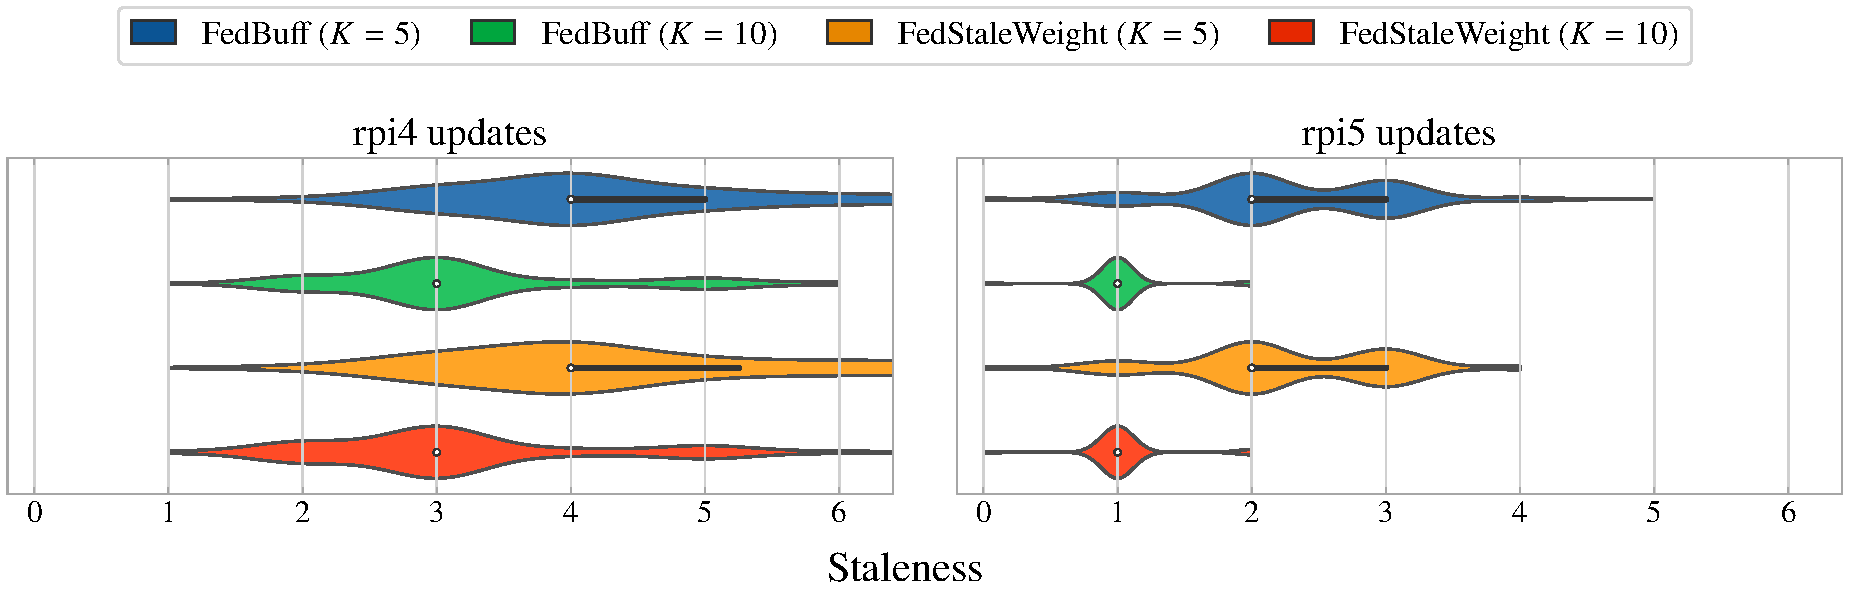
\includegraphics[width=0.98\textwidth]{figures/network_async_staleness_violin.pdf}
% Notes: panels split accepted updates by device class; each violin is one method--buffer setting.
% Inner bars show the interquartile range and the central marker shows the median.
% Distributions pool the first 60 server steps from seeds 1337--1339 for every method--buffer setting.
\caption{\textbf{Accepted-update staleness distributions in mixed non-IID runs.} Violins split accepted updates by device class and buffer setting.}
\label{fig:network_async_staleness_violin}
\end{figure}

Figure~\ref{fig:network_async_staleness_violin} confirms that \texttt{rpi4} updates are systematically staler than \texttt{rpi5} updates. \texttt{FedBuff} and \texttt{FedStaleWeight} have similar staleness distributions at the same \(K\), so their different behaviour comes mainly from the aggregation weights assigned after staleness weighting.


\begin{figure}[H]
\centering
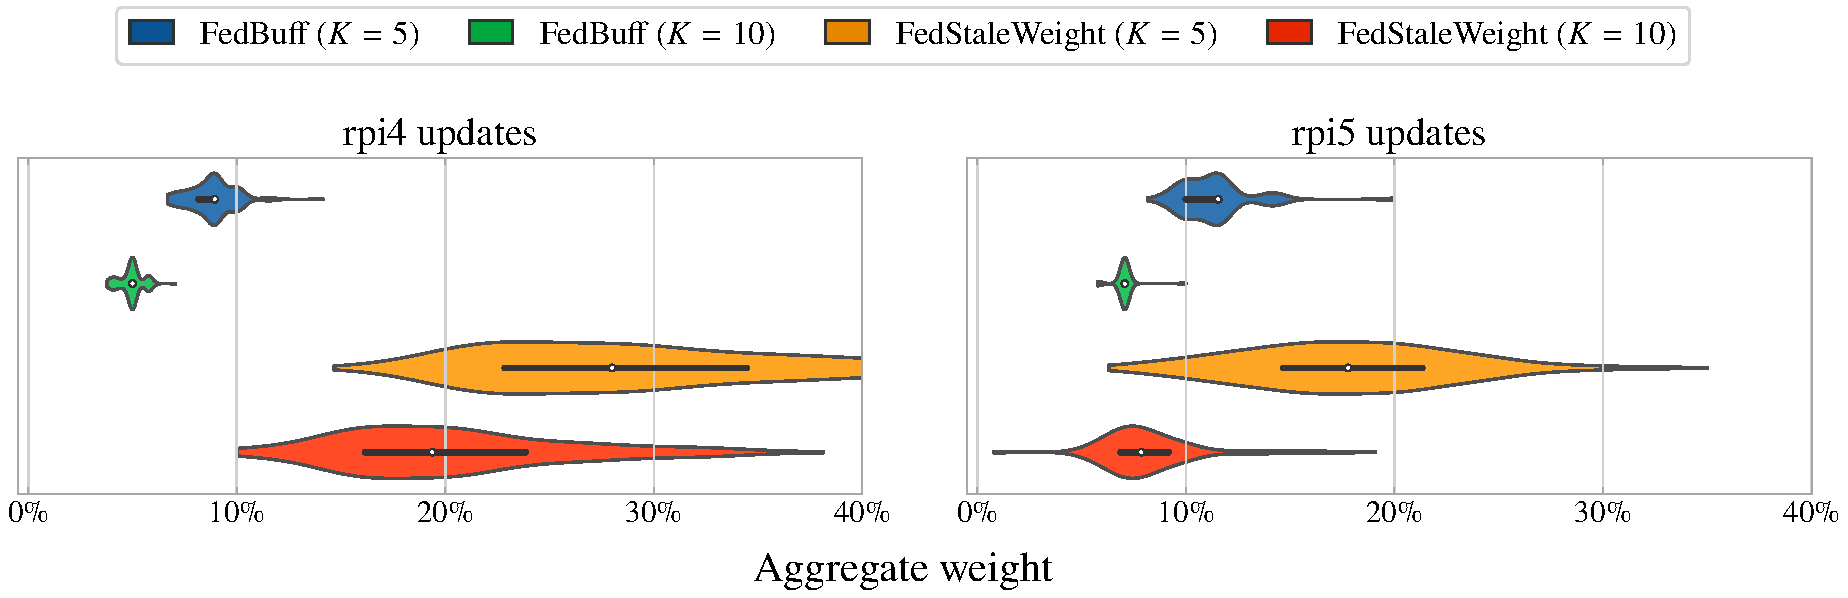
\includegraphics[width=0.98\textwidth]{figures/network_async_weight_violin.pdf}
% Notes: panels split accepted updates by device class.
% The x-axis shows the final aggregation weight assigned after the method-specific staleness rule.
% This separates update arrival frequency from server influence after weighting; seed coverage matches Figure~\ref{fig:network_async_staleness_violin}.
\caption{\textbf{Per-update aggregation weights in mixed non-IID runs.} Violins show the final weight assigned to each accepted update after method-specific staleness weighting, separating update frequency from server influence after weighting.}
\label{fig:network_async_weight_violin}
\end{figure}


Figure~\ref{fig:network_async_weight_violin} shows the difference: \texttt{FedBuff} gives accepted \texttt{rpi4} updates small weights, while \texttt{FedStaleWeight} shifts them into the \(20\)--\(30\%\) range. For \texttt{FedStaleWeight} with \(K=5\), that correction is broad and sometimes over-concentrated on a small set of stale updates, matching its instability in Table~\ref{tab:network_stressor_sweep}.


\paragraph{Takeaways.}
\begin{itemize}[leftmargin=*, nosep]
  \item Network stress mainly increases wall-clock time, but not client-trip count.
  \item \texttt{FedAsync} remains fastest to target under every stress profile, but its \texttt{rpi4} aggregate weight stays near \(8\%\) across profiles.
  \item \texttt{FedStaleWeight} with \(K=10\) is the best buffered representation compromise, while \(K=5\) makes \texttt{FedStaleWeight} unstable in this setting.
\end{itemize}

\FloatBarrier
\subsection{Stale-Aware Weighting Under Device-Correlated Skew}
\label{sec:eval_device_correlated_skew}

\paragraph{Setup.}
This subsection addresses \evalqref{S3} by testing \texttt{FedStaleWeight}'s core motivation: stale-aware weighting should offset slow-client under-representation when slower clients hold different data \parencite{ma2024fedstaleweight}. The ablation ties hardware speed to data: \texttt{rpi4} clients hold CIFAR-10 classes \(0\)--\(4\), while \texttt{rpi5} clients hold classes \(5\)--\(9\). This creates the case targeted by \texttt{FedStaleWeight}: slow clients arrive less often but carry distinct data, so stale-aware reweighting should increase their effective influence.

Table~\ref{tab:network_device_correlated} reports fixed-budget outcomes. \texttt{FedAvg} uses \(50\) rounds with \(15\) clients per round, for \(750\) completed trips; the asynchronous methods use \(150\) server steps with \(K=10\), for \(1500\) completed trips. This gives the asynchronous runs twice as many accepted updates, but \texttt{FedAvg} still takes longer in wall-clock time because each round waits for the slow clients.

\begin{table}[!htbp]
\centering
\scriptsize
% Notes: deployment uses 10 rpi5 + 5 rpi4 with no network impairment and device-correlated data heterogeneity.
% Results report mean +/- standard deviation over seeds 1337--1339.
% Class-group accuracies use seeds 1338--1339 only due to instrumentation availability.
% Accuracy is final centralized test accuracy at the configured budget.
% Class-group accuracies use held-out subsets corresponding to data predominantly assigned to rpi4 and rpi5 clients.
% Diagnostics report rpi4 accepted-update share, rpi4 aggregate-weight share, mean staleness by device, and updates per second; staleness and throughput cells report means only.
% Daggered values are structural synchronous values where update shares match population proportions and staleness is zero.
\caption{\textbf{Device-correlated non-IID fixed-budget ablation on CIFAR-10.} Outcomes are paired with class-group accuracies for labels held mainly by \texttt{rpi4} or \texttt{rpi5} clients.}
\label{tab:network_device_correlated}

\setlength{\tabcolsep}{2.9pt}
\begin{adjustbox}{max width=\textwidth}
\begin{tabular}{@{}lrrrrrrrrrr@{}}
\toprule
& \multicolumn{2}{c}{Fixed-budget outcome}
& \multicolumn{2}{c}{Class-group acc.}
& \multicolumn{2}{c}{\texttt{rpi4}}
& \multicolumn{2}{c}{Staleness}
& \\
\cmidrule(lr){2-3}
\cmidrule(lr){4-5}
\cmidrule(lr){6-7}
\cmidrule(lr){8-9}
Method
& \makecell{Wall\\clock (s)}
& \makecell{Final\\acc.}
& \makecell{\texttt{rpi4}\\held}
& \makecell{\texttt{rpi5}\\held}
& \makecell{update\\\%}
& \makecell{weight\\\%}
& \texttt{rpi4}
& \texttt{rpi5}
& \makecell{Updates/s} \\
\midrule
\texttt{FedAvg} & 8915 $\pm$ 596 & 40.8 $\pm$ 1.6 & 5.6 $\pm$ 2.6 & 75.8 $\pm$ 2.3 & 33.3$^\dagger$ & 33.3$^\dagger$ & 0$^\dagger$ & 0$^\dagger$ & 0.084 \\
\texttt{FedBuff} & \evalsecond{5840 $\pm$ 1613} & 40.8 $\pm$ 1.8 & 0.0 $\pm$ 0.0 & 80.6 $\pm$ 5.7 & 15.9 $\pm$ 2.5 & 12.2 $\pm$ 2.7 & 3.02 & 1.09 & 0.275 \\
\texttt{FedStaleWeight} & \evalbest{5813 $\pm$ 1588} & \evalbest{45.9 $\pm$ 1.3} & 12.9 $\pm$ 7.3 & 79.7 $\pm$ 5.9 & 15.7 $\pm$ 2.8 & 31.0 $\pm$ 0.3 & 3.08 & 1.09 & 0.276 \\
\texttt{FedAsync} & 7070 $\pm$ 19 & \evalsecond{43.0 $\pm$ 1.5} & 0.0 $\pm$ 0.0 & 86.1 $\pm$ 3.0 & 17.5 $\pm$ 0.1 & 11.9 $\pm$ 0.1 & 27.33 & 11.07 & 0.213 \\
\bottomrule
\end{tabular}
\end{adjustbox}
\end{table}

\paragraph{Interpretation.}
Despite being given twice as many completed trips, the asynchronous methods finish in less wall-clock time than \texttt{FedAvg}; device-correlated skew nevertheless remains hard. \texttt{FedStaleWeight} gives the best global accuracy at \(45.9 \pm 1.3\%\) and is the only method to noticeably improve the \texttt{rpi4}-held group, reaching \(12.9 \pm 7.3\%\). Even so, the device gap remains large: the \texttt{rpi5}-held group reaches roughly \(76\)--\(86\%\) accuracy, while the \texttt{rpi4}-held group is \(5.6 \pm 2.6\%\) for \texttt{FedAvg} and \(0.0 \pm 0.0\%\) for both \texttt{FedBuff} and \texttt{FedAsync}.

\begin{figure}[!htbp]
\centering
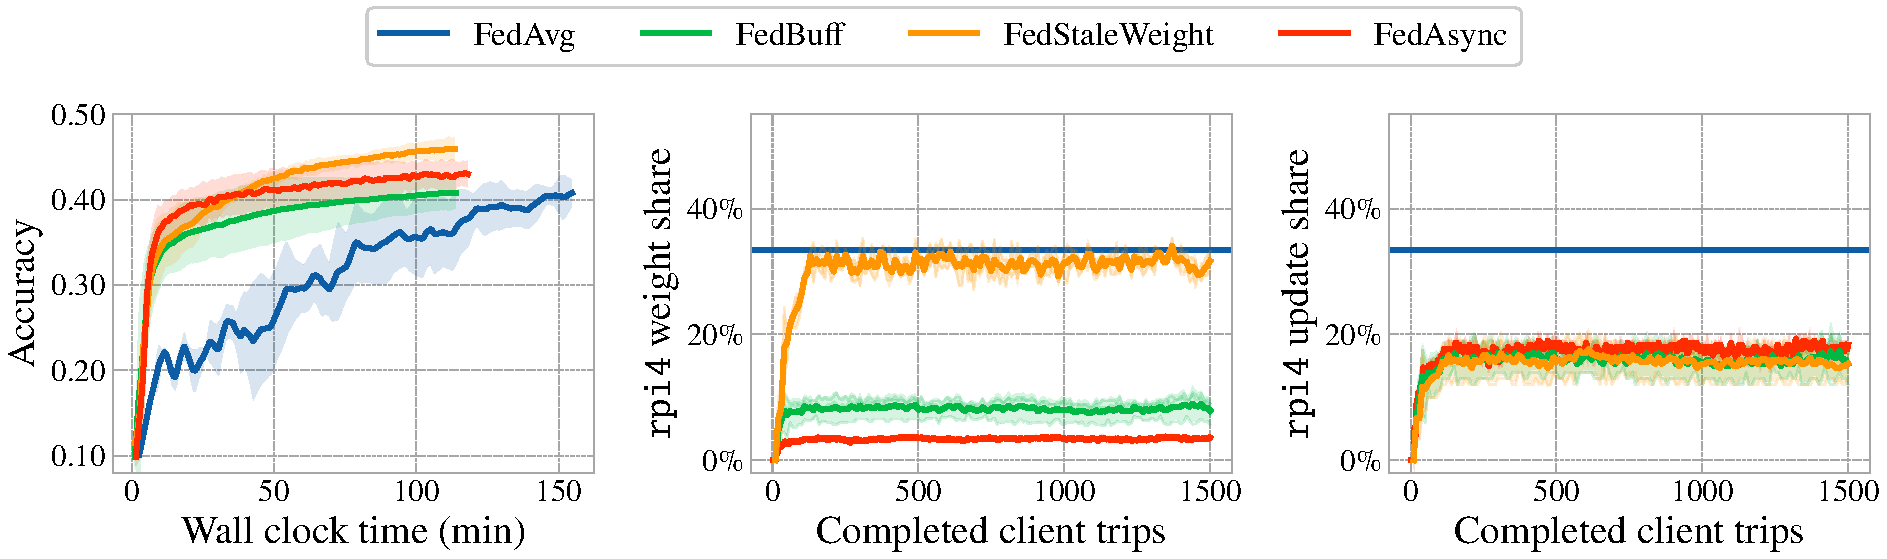
\includegraphics[width=\textwidth]{figures/network_device_correlated.pdf}
% Notes: the left panel shows three-seed mean centralized accuracy against wall-clock time with +/- one-standard-deviation bands.
% The middle and right panels show rpi4 weight and accepted-update shares over completed client trips.
% Faint traces are per-seed rolling means over a matched client-trip window; solid traces are their mean; shaded bands show +/- one standard deviation.
% The horizontal reference line in the share panels marks the structural rpi4 population share 5/15.
\caption{\textbf{Device-correlated non-IID accuracy and device-share diagnostics.} Traces separate slow-device update frequency from aggregate influence.}
\label{fig:network_device_correlated}
\end{figure}

Figure~\ref{fig:network_device_correlated} separates update frequency from aggregate influence. All asynchronous methods receive an \texttt{rpi4} update share below the \(33.3\%\) population share. \texttt{FedStaleWeight} raises \texttt{rpi4} aggregate weight close to population share and improves global accuracy, but it does not increase slow-client arrival frequency or recover strong \texttt{rpi4}-held class accuracy.

\paragraph{Takeaways.}
\begin{itemize}[leftmargin=*, nosep]
  \item Device-correlated skew is the hardest setting in this straggler-induced study: global accuracy remains low and the \texttt{rpi4}-held class group is poorly learned.
  \item \texttt{FedStaleWeight} improves global accuracy and slow-device aggregate influence, but the \texttt{rpi4}-held class group remains weak.
  \item Weighting stale updates helps representation but cannot replace more frequent slow-client participation or data-aware correction.
\end{itemize}

\FloatBarrier
\section{Asynchronous Submodel Federated Learning}
\label{sec:eval_async_submodel_fl}

The previous sections evaluate synchronous submodel training and standard asynchronous training separately. This section combines them and tests \texttt{FedCover} from Section~\ref{sec:fedcover_impl}, using accepted asynchronous submodel buffers to measure parameter coverage during aggregation.

\FloatBarrier
\subsection{Feasibility Across Tasks and Data Regimes}

\paragraph{Setup.}
This subsection addresses \evalqref{A1}: whether asynchronous submodel FL is feasible across tasks and data regimes. The comparison uses the same \(20\)-node mixed deployment and nested \texttt{HeteroFL} rate assignment as the compute benchmark. Methods are synchronous \texttt{HeteroFL}, coverage-disabled asynchronous \texttt{HeteroFL} labelled \texttt{Async-HeteroFL}, \texttt{FedCover}, and \texttt{FedBuff}; \texttt{Async-HeteroFL} is the direct buffered composition isolating \texttt{FedCover}'s coverage correction. Unlike workload-adaptive approaches such as \texttt{TimelyFL}, this experiment keeps the nested rate assignment fixed and tests aggregation-side coverage. Appendix~\ref{appendix:evaluation_settings}, Table~\ref{tab:appendix_fedcover_settings}, lists run settings. All \texttt{FedCover} rows use \(\kappa_{\max}=3\), so sweep differences reflect \(\gamma\), not the correction cap.

\paragraph{Interpretation.}
The table shows that the combined setting is operationally feasible rather than merely a conceptual composition. Asynchronous submodel variants reach target in all CIFAR-10 runs, including the non-IID regime where synchronous \texttt{HeteroFL} reaches the \(60\%\) target for only \(2/3\) seeds. Fashion-MNIST shows the same feasibility pattern under IID data and a harder non-IID case: every cap-matched \texttt{FedCover} setting reaches the \(75\%\) target for every seed, while the synchronous and coverage-disabled baselines each have at least one censored seed. \texttt{FedBuff} is retained as an asynchronous reference, but it is not capacity-matched to the submodel methods and is therefore unranked.


\paragraph{Takeaways.}
\begin{itemize}[leftmargin=*, nosep]
  \item Asynchronous submodel FL is feasible across the CIFAR-10 and Fashion-MNIST settings.
  \item Non-IID Fashion-MNIST is the hardest feasibility case, with censored seeds for the synchronous and coverage-disabled baselines.
  \item \texttt{Async-HeteroFL} is the controlled coverage-disabled baseline for the next subsection; \texttt{FedBuff} remains contextual because it is not capacity-matched.
\end{itemize}

\begin{table}[H]
\centering
\scriptsize
\renewcommand{\arraystretch}{1.02}
\setlength{\tabcolsep}{2pt}
% Notes: values are mean +/- standard deviation over seeds 1337--1339.
% The target is first centralized accuracy >= the task/data target stated in the surrounding paragraph.
% Daggered trip/time cells are lower-bound aggregates: one or more seeds did not reach target, so the final observed run point was substituted.
% Post-warm-up time subtracts the first 20 completed client trips: one synchronous HeteroFL round or five async buffered server steps.
% rpi4 weight share is aggregate server weight assigned to rpi4 updates; synchronous HeteroFL has the structural 50% share.
% Coverage gain is the mean FedCover multiplicative correction; the daggered async-HeteroFL value is the disabled-correction baseline.
% All FedCover rows use kappa_max = 3; gamma is the swept coverage-power parameter.
% FedBuff is a higher-capacity full-model asynchronous reference, not a capacity-matched baseline.
\caption{\textbf{Asynchronous submodel FL with coverage-aware aggregation.} Target metrics use task-specific IID/non-IID thresholds; all \texttt{FedCover} rows use \(\kappa_{\max}=3\).}  
\label{tab:fedcover_async_submodel}
\begin{adjustbox}{max width=\textwidth}
\begin{tabular}{@{}lllccccc@{}}
\toprule
Task & Data & Method & \makecell{Trips\\to target} & \makecell{Time to\\target (min)} & \makecell{Post-warm-up\\target (min)} & \makecell{\texttt{rpi4}\\weight (\%)} & \makecell{Coverage\\gain} \\
\midrule
\multirow{14}{*}{\makecell[l]{CIFAR-10}} & \multirow{7}{*}{IID} & \texttt{FedBuff}\(^*\) & \(120\pm0\) & \(35.7\pm7.5\) & \(19.8\pm0.3\) & \(34.3\pm0.7\) & -- \\
 &  & \texttt{HeteroFL} & \(193\pm12\) & \(24.2\pm2.9\) & \(18.3\pm2.7\) & \(50.0\pm0.0\) & -- \\
 &  & \texttt{Async-HeteroFL} & \(227\pm12\) & \(33.9\pm16.0\) & \(18.4\pm1.8\) & \(44.5\pm0.3\) & \(1.00^\dagger\) \\
 &  & \texttt{FedCover} \((\gamma=0.25)\) & \(193\pm12\) & \(19.9\pm0.6\) & \(15.2\pm1.4\) & \(44.9\pm0.5\) & \(1.23\pm0.11\) \\
 &  & \texttt{FedCover} \((\gamma=0.5)\) & \(167\pm12\) & \(17.1\pm0.9\) & \(12.7\pm1.1\) & \(44.0\pm2.8\) & \(2.03\pm0.56\) \\
 &  & \texttt{FedCover} \((\gamma=1.0)\) & \evalsecond{\(133\pm12\)} & \evalsecond{\(13.8\pm0.6\)} & \evalsecond{\(9.7\pm0.9\)} & \(43.6\pm1.3\) & \(2.65\pm0.06\) \\
 &  & \texttt{FedCover} \((\gamma=1.5)\) & \evalbest{\(127\pm12\)} & \evalbest{\(13.7\pm2.1\)} & \evalbest{\(9.3\pm1.1\)} & \(42.6\pm0.6\) & \(2.73\pm0.17\) \\
\cmidrule(l){2-8}
 & \multirow{7}{*}{Non-IID} & \texttt{FedBuff}\(^*\) & \(133\pm12\) & \(30.2\pm3.3\) & \(19.1\pm3.5\) & \(32.6\pm1.4\) & -- \\
 &  & \texttt{HeteroFL} & \evalcensored{420\pm80} & \evalcensored{51.6\pm19.2} & \evalcensored{39.3\pm12.5} & \(50.0\pm0.0\) & -- \\
 &  & \texttt{Async-HeteroFL} & \(400\pm35\) & \(38.2\pm9.1\) & \(29.2\pm3.9\) & \(45.0\pm2.3\) & \(1.00^\dagger\) \\
 &  & \texttt{FedCover} \((\gamma=0.25)\) & \(380\pm151\) & \(31.3\pm11.4\) & \(27.5\pm11.4\) & \(43.6\pm1.1\) & \(1.27\pm0.08\) \\
 &  & \texttt{FedCover} \((\gamma=0.5)\) & \(273\pm31\) & \(23.1\pm2.7\) & \(19.4\pm2.7\) & \(45.0\pm1.5\) & \(2.22\pm0.36\) \\
 &  & \texttt{FedCover} \((\gamma=1.0)\) & \evalsecond{\(220\pm92\)} & \evalsecond{\(18.8\pm7.1\)} & \evalsecond{\(15.3\pm7.1\)} & \(43.3\pm1.4\) & \(2.81\pm0.10\) \\
 &  & \texttt{FedCover} \((\gamma=1.5)\) & \evalbest{\(187\pm12\)} & \evalbest{\(16.3\pm0.3\)} & \evalbest{\(12.8\pm0.4\)} & \(44.2\pm2.6\) & \(2.91\pm0.08\) \\
\midrule
\multirow{14}{*}{\makecell[l]{Fashion\\MNIST}} & \multirow{7}{*}{IID} & \texttt{FedBuff}\(^*\) & \(160\pm20\) & \(7.2\pm0.7\) & \(5.3\pm0.7\) & \(36.1\pm0.8\) & -- \\
 &  & \texttt{HeteroFL} & \(273\pm23\) & \(12.9\pm1.1\) & \(12.0\pm1.1\) & \(50.0\pm0.0\) & -- \\
 &  & \texttt{Async-HeteroFL} & \(347\pm42\) & \(11.8\pm1.4\) & \(10.1\pm1.4\) & \(41.2\pm0.6\) & \(1.00^\dagger\) \\
 &  & \texttt{FedCover} \((\gamma=0.25)\) & \(307\pm12\) & \(10.6\pm0.4\) & \(8.9\pm0.4\) & \(42.1\pm0.8\) & \(1.42\pm0.10\) \\
 &  & \texttt{FedCover} \((\gamma=0.5)\) & \(240\pm20\) & \(8.6\pm0.7\) & \(6.9\pm0.7\) & \(40.3\pm1.5\) & \(1.99\pm0.51\) \\
 &  & \texttt{FedCover} \((\gamma=1.0)\) & \evalsecond{\(167\pm12\)} & \evalsecond{\(6.2\pm0.3\)} & \evalsecond{\(4.5\pm0.3\)} & \(39.4\pm0.4\) & \(2.93\pm0.04\) \\
 &  & \texttt{FedCover} \((\gamma=1.5)\) & \evalbest{\(160\pm20\)} & \evalbest{\(6.0\pm0.7\)} & \evalbest{\(4.4\pm0.6\)} & \(38.6\pm0.6\) & \(2.93\pm0.06\) \\
\cmidrule(l){2-8}
 & \multirow{7}{*}{Non-IID} & \texttt{FedBuff}\(^*\) & \(180\pm40\) & \(7.7\pm1.5\) & \(5.9\pm1.5\) & \(35.6\pm3.0\) & -- \\
 &  & \texttt{HeteroFL} & \evalcensored{473\pm46} & \evalcensored{22.6\pm2.8} & \evalcensored{21.8\pm2.9} & \(50.0\pm0.0\) & -- \\
 &  & \texttt{Async-HeteroFL} & \evalcensored{613\pm167} & \evalcensored{20.5\pm6.4} & \evalcensored{18.8\pm6.4} & \(38.7\pm1.5\) & \(1.00^\dagger\) \\
 &  & \texttt{FedCover} \((\gamma=0.25)\) & \(607\pm214\) & \(19.4\pm6.3\) & \(17.8\pm6.2\) & \(39.3\pm2.3\) & \(1.45\pm0.11\) \\
 &  & \texttt{FedCover} \((\gamma=0.5)\) & \(467\pm76\) & \evalsecond{\(15.2\pm2.3\)} & \(13.5\pm2.3\) & \(39.8\pm1.3\) & \(1.71\pm0.12\) \\
 &  & \texttt{FedCover} \((\gamma=1.0)\) & \evalsecond{\(460\pm296\)} & \(15.5\pm9.9\) & \evalsecond{\(13.4\pm9.0\)} & \(39.9\pm2.9\) & \(2.46\pm0.53\) \\
 &  & \texttt{FedCover} \((\gamma=1.5)\) & \evalbest{\(327\pm76\)} & \evalbest{\(11.0\pm2.3\)} & \evalbest{\(9.3\pm2.3\)} & \(39.9\pm1.0\) & \(2.90\pm0.12\) \\
\bottomrule
\end{tabular}
\end{adjustbox}
\par\vspace{0.2em}
{\centering\scriptsize \(\ddagger\) lower-bound aggregate: at least one seed did not reach target. \\ \(^*\)\texttt{FedBuff} is a full-model, higher-capacity asynchronous baseline reference and is thus unranked.\par}
\end{table}


\FloatBarrier
\subsection{Coverage-Aware Aggregation with FedCover}
\label{sec:eval_coverage_mismatch}

\paragraph{Setup.}
Building on the same runs reported in Table~\ref{tab:fedcover_async_submodel}, this subsection addresses \evalqref{A2}: whether \texttt{FedCover}'s coverage correction improves asynchronous submodel FL. The capacity-matched comparison is synchronous \texttt{HeteroFL}, coverage-disabled asynchronous \texttt{HeteroFL}, and \texttt{FedCover} across \(\gamma\) values. \texttt{FedBuff} remains an asynchronous reference rather than a capacity-matched baseline.

\paragraph{Interpretation.}
On CIFAR-10 IID, \texttt{FedCover} gives the clearest target-time improvement among capacity-matched methods: \(\gamma=1.5\) reduces mean time to target from \(24.2\) minutes for synchronous \texttt{HeteroFL} and \(33.9\) minutes for coverage-disabled asynchronous \texttt{HeteroFL} to \(13.7\) minutes, with the lowest trip count and post-warm-up target time. With the cap fixed, \(\gamma=1.0\) is now close behind at \(13.8\) minutes and \(9.7\) post-warm-up minutes. The non-IID setting strengthens the need for the larger correction: \(\gamma=1.5\) reaches the \(60\%\) target in \(16.3\) minutes, compared with \(38.2\) minutes for the coverage-disabled asynchronous baseline and \(18.8\) minutes for \(\gamma=1.0\).

Fashion-MNIST repeats the same main pattern on a second image task. In IID, \(\gamma=1.5\) reaches the \(80\%\) target in \(6.0\) minutes and reduces post-warm-up time to \(4.4\) minutes, only slightly ahead of \(\gamma=1.0\). In non-IID, \(\gamma=1.5\) is again the strongest target-time setting; \(\gamma=1.0\) has the second-best post-warm-up mean, while \(\gamma=0.5\) is marginally second on total target time.

Figure~\ref{fig:fedcover_post_warmup_speedup} makes the post-warm-up pattern clearer. Every \(\gamma\) setting has positive mean speedup over coverage-disabled \texttt{Async-HeteroFL} after warm-up. The IID panels show the cleanest trend: larger \(\gamma\) and larger observed coverage gain \(\bar{\kappa}\) give consistent speedup, with \(\gamma=1.0\) close to \(\gamma=1.5\). The non-IID panels are more seed-sensitive for weaker corrections, but \(\gamma=1.5\) gives the largest average speedup in both tasks, reaching roughly \(56\%\) on CIFAR-10 and \(48\%\) on Fashion-MNIST. This supports the interpretation that \texttt{FedCover} is compensating for under-covered parameter blocks after warm-up, while also showing that the strongest correction matters most under data skew. Its \texttt{rpi4} aggregate weight remains close to the coverage-disabled asynchronous baseline, so the improvement comes from coverage-aware aggregation rather than simply increasing slow-device aggregate weight.

\begin{figure}[!htbp]
\centering
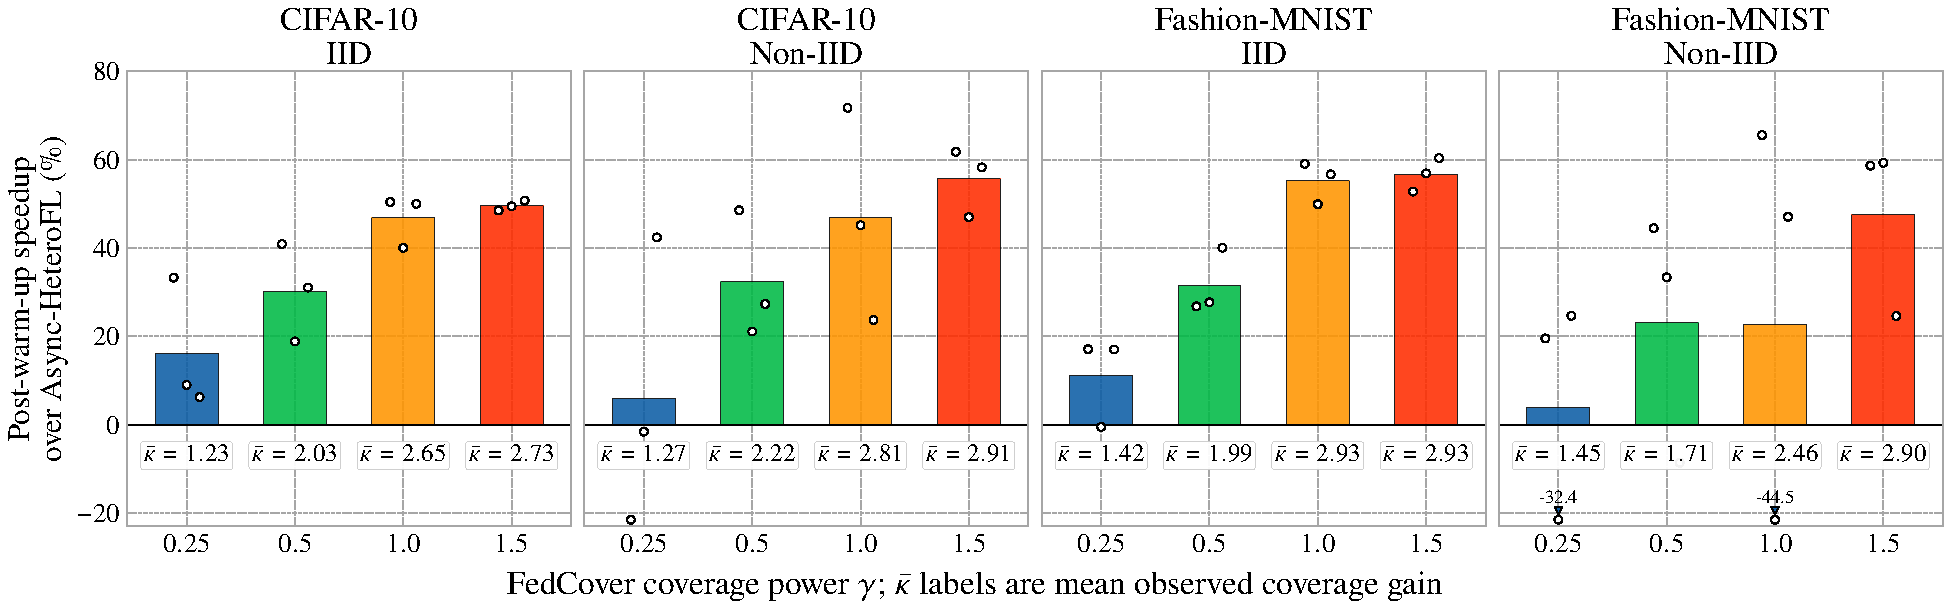
\includegraphics[width=\textwidth]{figures/fedcover_post_warmup_speedup.pdf}
\caption{\textbf{Post-warm-up speedup from coverage-aware aggregation.} Bars show mean paired-seed speedup over coverage-disabled \texttt{Async-HeteroFL}; open circles show seeds.}
\label{fig:fedcover_post_warmup_speedup}
\end{figure}

\paragraph{Takeaways.}

\begin{itemize}[leftmargin=*, nosep]
  \item \texttt{FedCover} improves the coverage-disabled \texttt{Async-HeteroFL} baseline across all task--regime pairs, especially in target time and post-warm-up time.
  \item With \(\kappa_{\max}\) fixed, \(\gamma=1.0\) nearly matches \(\gamma=1.5\) on IID data, while \(\gamma=1.5\) is strongest under non-IID data.
  \item The gains are not explained by slow-device reweighting: \texttt{rpi4} aggregate weight stays close to \texttt{Async-HeteroFL}, so the improvement is consistent with correcting under-covered parameter blocks.
\end{itemize}

\FloatBarrier
% \subsection{Platform and Reproducibility Evidence}

% The execution path is also part of the evaluated contribution. The headline compute-heterogeneity and straggler-induced heterogeneity evaluations were launched through the same \texttt{fedctl submit} path: a Flower run config defined the learning problem and method parameters, while a deploy config defined placement, device type, oversubscription, and optional \texttt{netem} impairment. This split is what made the controls above practical: the network-stressor sweep changed the deployment-side impairment while preserving the learning configuration, and the compute-heterogeneity experiments changed model-rate assignment while preserving the mixed rack.

% Each submission preserved the reconstructed request, run config, deploy config, Nomad jobs, logs, W\&B metrics, and result artifacts. This matters scientifically because failed, censored, or rerun experiments remain inspectable rather than disappearing as terminal cluster jobs. The corrected mixed-topology network reruns are the clearest example: the stored submission state made the placement error visible and allowed the affected runs to be repeated under the intended mixed topology.

% Overall, the evaluation supports three conclusions. First, submodel FL is useful on the live Raspberry Pi rack when local compute is a real bottleneck, but the best method depends on whether the objective is quality or speed: \texttt{FIARSE} gives stronger submodel quality, while \texttt{HeteroFL} and \texttt{FedRolex} give clearer wall-clock savings. Second, asynchronous coordination is not uniformly better than synchronous training; it helps mainly when completion times are heterogeneous, and its advantage is primarily a wall-clock effect rather than a universal reduction in client trips. Third, stale-aware weighting can restore the aggregate influence of slow devices, but it does not make those devices participate more often. Device-correlated data skew therefore remains difficult and is not solved by weighting alone.

% !TeX root = main.tex
\chapter{Conclusions}
\label{chap:conclusions}

This dissertation developed \texttt{fedctl}, built a Raspberry Pi cluster with \(30\) \texttt{rpi4} and \(20\) \texttt{rpi5} workers, evaluated heterogeneous FL methods under realistic deployment conditions, and proposed \texttt{FedCover} for asynchronous submodel FL. The central argument is that heterogeneous FL methods must be evaluated through both model performance and deployment behaviour, since deployment factors such as device capability, memory constraints, update timing, network conditions, submodel quality, and parameter coverage shape outcomes.

Taken together, the results support three claims. Firstly, compute and straggler-induced heterogeneity create trade-offs between wall-clock time, client participation, submodel quality, and fairness. Secondly, asynchronous submodel FL is feasible without redesigning either underlying method family, but partial, asynchronous replies make parameter coverage an important factor in aggregation. Thirdly, \texttt{FedCover}'s capped inverse-coverage correction improves time-to-target performance relative to uncorrected \texttt{Async-HeteroFL}.

\section{Work completed}

\paragraph{1. Developed \texttt{fedctl}: a tool for deployed FL evaluation.} \hangindent=2em
To fulfil main aim~\hyperref[aim:a]{(a)}, I designed and implemented \texttt{fedctl} as the tool used to run and inspect the experiments in Chapter~\ref{chap:evaluation}. It packages a Flower application, records the effective run and deploy configs, submits the request to a queued service, and launches the corresponding Nomad jobs on the Raspberry Pi cluster. The CLI and browser surfaces expose queue state, logs, artefacts, and results, while the run-config/deploy-config split keeps method choices separate from placement, resources, and network conditions. This made the evaluation reproducible rather than dependent on ad hoc launch scripts.

\paragraph{2. Built a heterogeneous Raspberry Pi cluster for deployed FL evaluation.} \hangindent=2em
To fulfil main aim~\hyperref[aim:b]{(b)}, I built and provisioned a Raspberry Pi cluster with \(30\) \texttt{rpi4} and \(20\) \texttt{rpi5} workers, configured with Ansible and orchestrated through Nomad. \texttt{fedctl} exposes the cluster as typed workers, applies controlled \texttt{netem} impairment, and records device-labelled diagnostics. The testbed turns physical heterogeneity into controlled experimental variables with a traceable evidence path through configuration, logs, W\&B metrics, artefacts, and runtime metadata.

\paragraph{3. Evaluated compute heterogeneity with submodel FL.} \hangindent=2em
To fulfil main aim~\hyperref[aim:c]{(c)}, I implemented and evaluated \texttt{FedAvg}, \texttt{HeteroFL}, \texttt{FedRolex}, and \texttt{FIARSE}, covering aim~\hyperref[aim:c.1]{(c.1)}--\hyperref[aim:c.3]{(c.3)}. Section~\ref{sec:eval_compute_heterogeneity} showed that submodel FL helps when local compute is the bottleneck, but the best method depends on the objective: \texttt{FedAvg} remains the full-model quality control, \texttt{FIARSE} gives the strongest deployable submodel quality, and \texttt{HeteroFL}/\texttt{FedRolex} give the clearest wall-clock savings.

\paragraph{4. Evaluated straggler-induced heterogeneity with asynchronous FL.} \hangindent=2em
To fulfil extension aims~\hyperref[eaim:a]{(a)} and \hyperref[eaim:b]{(b)}, I evaluated straggler-induced heterogeneity using synchronous \texttt{FedAvg} as a reference and asynchronous \texttt{FedAsync}, \texttt{FedBuff}, and \texttt{FedStaleWeight} under mixed completion times and controlled network conditions. Section~\ref{sec:eval_network_heterogeneity} showed that asynchronous updates are useful mainly when client completion times differ: in all-\texttt{rpi5} controls, synchronous \texttt{FedAvg} remains the stronger target-attainment baseline, while mixed \texttt{rpi4}/\texttt{rpi5} runs make \texttt{FedAsync} fastest and \texttt{FedStaleWeight} better at restoring slow-device influence.

\paragraph{5. Combined asynchronous FL with submodel FL and proposed \texttt{FedCover}.} \hangindent=2em
To fulfil extension aims~\hyperref[eaim:c]{(c)} and \hyperref[eaim:d]{(d)}, I evaluated buffered asynchronous aggregation over nested submodel updates and introduced \texttt{FedCover} in Section~\ref{sec:fedcover_impl}. Unlike workload-adaptive prior work \parencite{zhang2023timelyfl}, this dissertation fixes the nested model-rate assignment and isolates aggregation-side coverage correction. Section~\ref{sec:eval_async_submodel_fl} shows that the direct composition, \texttt{Async-HeteroFL}, is feasible, but stale-weighted buffers make parameter coverage dynamic. \texttt{FedCover}'s capped inverse-coverage correction improves time to target while leaving slow-device representation close to the uncorrected baseline.

\section{Future work}
\label{sec:future_work}

\paragraph{Broader workloads, devices, and runtimes.} \hangindent=2em
The evaluated workloads expose compute and runtime trade-offs on CPU-only Raspberry Pi clients, but leave broader tasks and heterogeneous devices open \parencite{caldas2018leaf,lai2022fedscale,li2021ditto}. Future work should test whether the same trade-offs hold on a wider client-device mix, including accelerators such as NVIDIA Jetson Nano devices and Raspberry Pi 5 QPU runtimes.

\paragraph{Representation-aware asynchronous training.} \hangindent=2em
Weighting stale updates can improve slow-device influence, but it cannot make slow clients arrive more often. Device-correlated skew therefore needs methods that combine staleness weighting with fairness-aware objectives, device-aware admission, client selection, or data-aware scheduling \parencite{li2019qffl,nishio2018fedcs,lai2021oort,chai2020tifl}.

\paragraph{Hardware-aware submodel execution.} \hangindent=2em
\texttt{FIARSE} improves submodel quality here, but executes sparse masks through dense PyTorch kernels on edge CPUs. Future work should separate the algorithmic value of sparse importance-selected submodels from the systems cost of executing them without sparse-kernel or hardware support.

\paragraph{Trace-driven straggler-induced heterogeneity evaluation.} \hangindent=2em
The \texttt{netem} make impairment reproducible, but they remain controlled approximations of real deployment conditions. Future work should replay measured edge-network traces through the same \texttt{fedctl} path, connecting controlled profiles with real path variability \parencite{bonawitz2019towards,lai2022fedscale}.

% This dissertation argues that FL systems should be evaluated as deployed distributed systems rather than idealised statistical abstractions.

\label{lastcontentpage}

\addcontentsline{toc}{chapter}{Bibliography}
\begingroup
\setlength{\emergencystretch}{2em}
\printbibliography
\endgroup

\appendix
% !TeX root = main.tex
\chapter{Notation Reference}
\label{chap:notation}

This appendix summarises the main notation used throughout the dissertation. The goal is not to restate every paper-specific symbol, but to keep the shared notation for the synchronous, submodel, and buffered-asynchronous methods in one place.

\section*{General Federated Learning}
\vspace{-1em}
\begin{longtable}{@{} p{0.18\linewidth} p{0.78\linewidth} @{}}
$\mathcal{K}$ & Set of all available clients. \\
$\mathcal{C}_t$ & Client set selected in synchronous round $t$. \\
$t$ & Synchronous communication-round index. \\
$s$ & Buffered-asynchronous server-step index. \\
$T$ & Total number of synchronous rounds. \\
$S$ & Total number of asynchronous server steps. \\
$w^{(t)}$ & Global model after synchronous round $t$. \\
$w^{[s]}$ & Global model after asynchronous server step $s$. \\
$[w]_j$ & Coordinate \(j\) of model \(w\); bracket notation distinguishes parameter coordinates from client-indexed models such as \(\tilde{w}_k\). \\
$D_k$ & Local training dataset stored on client $k$. \\
$n_k$ & Number of training examples used by client $k$. \\
$p_k$ & Client weight in the global objective; FedAvg normalisation over the selected client set is written explicitly over $\mathcal{C}_t$ in the main text. \\
$F_k(w)$ & Local objective of client $k$. \\
$F(w)$ & Global objective, typically $F(w)=\sum_{k \in \mathcal{K}} p_k F_k(w)$. \\
$\eta_\ell$ & Client-side learning rate for local optimisation. \\
$\eta_s$ & Server-side learning rate used in aggregation updates. \\
$E$ & Number of local epochs per synchronous round. \\
$\tilde{w}_k^{(t+1)}$ & Local model returned by client $k$ after training from synchronous global model $w^{(t)}$. \\
\end{longtable}

\section*{Submodel Training}
\vspace{-1em}
\begin{longtable}{@{} p{0.18\linewidth} p{0.78\linewidth} @{}}
$r_k$ & Fixed model rate assigned to client $k$. \\
$I_k^{(t)}$, $I_k^{[s]}$ & Parameter subset visible to client $k$ in synchronous round $t$ or asynchronous dispatch step $s$. \\
$w_{k,0}^{(t)}$ & Client-visible model or submodel used by client $k$ before local training. \\
$\mathcal{U}_j^{(t)}$ & Set of participating clients whose extracted submodels include global parameter $j$ at round $t$. \\
$\Psi$, $\Psi_{\mathcal{M}}$ & Method-specific extraction policy that maps a global model, model rate, and round index to the client-visible submodel indices. \\
$s_j^{(t)}$ & Magnitude-based importance score assigned to parameter $j$ for the \texttt{FIARSE} sparse mask in round \(t\). \\
\end{longtable}

\section*{Buffered-Asynchronous Training}
\vspace{-1em}
\begin{longtable}{@{} p{0.18\linewidth} p{0.78\linewidth} @{}}
$M$ & Maximum number of concurrent in-flight client requests in buffered asynchronous execution. \\
$K$ & Buffer size used by the server before applying an asynchronous update. \\
$\mathcal{B}$ & Mutable set of accepted updates currently stored in the async buffer. \\
$\mathcal{B}_s$ & Accepted buffer whose aggregate is applied at asynchronous server step $s$. \\
$v_i$ & Model version originally sent to the client that produced async update $i$. \\
$\Delta_i$ & Delta associated with async update $i$, using the sign convention $\Delta_i=w^{[v_i]}-\tilde{w}_i$. \\
$[\Delta_i]_j$, $[\bar{\Delta}^{[s]}]_j$ & Coordinate \(j\) of an individual async delta or buffered aggregate delta. \\
$\tau_i$ & Staleness of async update $i$, measured in server steps since version $v_i$. \\
$q_i$ & Nonnegative staleness score assigned to buffered async update $i$ before normalisation. \\
$\alpha_i$ & Normalised buffer weight applied to buffered async update $i$, usually $\alpha_i=q_i/\sum_{u\in\mathcal{B}_s}q_u$. \\
$g(\tau_i)$ & Staleness-weighting function used to construct a buffered score from update staleness. \\
\end{longtable}

\section*{Method-Specific Parameters}
\vspace{-1em}
\begin{longtable}{@{} p{0.18\linewidth} p{0.78\linewidth} @{}}
$a$ & Polynomial staleness-decay exponent for the weighted \texttt{FedBuff} variant. \\
$c_j^{[s]}$ & Observed stale-weighted coverage mass for parameter $j$ in accepted buffer $\mathcal{B}_s$. \\
$\gamma$ & FedCover coverage-gain exponent. \\
$\kappa_{\max}$ & Maximum FedCover inverse-coverage gain. \\
$\kappa_j^{[s]}$ & Capped inverse-coverage gain applied to parameter $j$ at server step $s$. \\
\end{longtable}

% !TeX root = main.tex
%TC:ignore
\chapter{Core Systems Concepts}
\label{appendix:systems_definitions}

This appendix defines the systems terms used in the implementation chapter. The definitions are intentionally operational: they explain how each concept is used in this dissertation, rather than documenting every feature of the underlying tool.

\section{Flower}
\label{def:flower}

\begin{definition}
\textbf{Flower.}
Flower is an open-source framework for defining and running federated-learning workloads \parencite{beutel2022flower}. In this dissertation, Flower is the layer in which the server-side coordination logic and client-side training logic are written; \texttt{fedctl} supplies the surrounding deployment path that places those roles on the cluster, configures them, and preserves the resulting evidence.
\end{definition}

Flower separates the project-specific learning logic from the runtime processes that connect a federation. A Flower project can therefore be run locally for development or connected to a remote federation in which server-side and client-side work execute as separate processes. \texttt{fedctl} uses this separation: it keeps the learning problem inside the Flower project, while controlling placement, network conditions, images, logs, and artifacts outside Flower.

\section{Flower Runtime Components}
\label{def:flower_components}

The implementation chapter refers to the following Flower-facing roles. The wording here is a dissertation-specific summary of Flower's deployment architecture,\footnote{\href{https://flower.ai/docs/framework/explanation-flower-architecture.html}{Flower architecture documentation}.} focused on the concepts needed to understand \texttt{fedctl}.

\begin{description}[leftmargin=2.8cm, style=nextline]
  \item[SuperLink] The central communication service for a Flower federation. It is the rendezvous point between server-side app execution and the connected client-side runtime endpoints; it routes run instructions and results, but does not contain the learning method.
  \item[SuperNode] The client-side runtime endpoint in a Flower federation. It connects to the SuperLink and exposes a client endpoint that can be selected for work during a run; it is the runtime presence of a client, not the client training code itself.
  \item[ServerApp] The project-specific server-side application for a run. It contains the logic that starts and coordinates the FL workload, including client selection, aggregation, global evaluation, and server-side metric logging.
  \item[ClientApp] The project-specific client-side application executed for selected client work. It loads the assigned local data, performs local training or evaluation, and returns model updates and metrics.
  \item[SuperExec] The executor process that runs a \texttt{ServerApp} or \texttt{ClientApp} and connects that app process to the corresponding Flower runtime endpoint. In \texttt{fedctl}, ServerApp and ClientApp SuperExec containers are the application jobs rendered into Nomad.
\end{description}

The term \emph{logical client} refers to the client identity used by the FL experiment. In this deployment, each logical client is realised by a paired SuperNode endpoint and ClientApp SuperExec job. A logical client need not be the same thing as a physical machine: \texttt{fedctl} maps logical clients to physical devices through deployment configuration and Nomad placement, then records the device label with the resulting metrics.

\section{Nomad}
\label{def:nomad}

\begin{definition}
\textbf{Nomad.}
Nomad is a cluster scheduler from HashiCorp used to place and run containerised jobs across a pool of machines \parencite{nomad}. In this dissertation, Nomad is the execution substrate beneath Flower: \texttt{fedctl} renders Flower roles into Nomad jobs, adds placement constraints and resource reservations, and submits those jobs to the Raspberry Pi cluster.
\end{definition}

The main Nomad terms used in Chapter~\ref{chap:implementation} are:

\begin{description}[leftmargin=2.8cm, style=nextline]
  \item[Job] A submitted unit of work. \texttt{fedctl} renders separate jobs for Flower runtime services, application executors, and submit-runner work.
  \item[Task group] A group of tasks that Nomad schedules together. \texttt{fedctl} uses task groups to represent repeated logical-client roles such as SuperNodes.
  \item[Allocation] A concrete placement of a task group on a physical Nomad client node.
  \item[Constraint] A scheduling rule. Device-aware placement uses constraints such as matching a requested worker type to Nomad node metadata.
  \item[Service] A named network endpoint registered by a running task. Flower roles discover each other through these services rather than through hard-coded IP addresses.
\end{description}

Nomad does not implement the FL algorithm. It decides where the runtime processes execute, reserves resources, exposes service addresses, and reports operational state. This is why the implementation chapter distinguishes the Flower method layer from the Nomad deployment layer.

\section{Containers, Registry, and Submit Runner}
\label{def:containers_registry_submit_runner}

\begin{definition}
\textbf{Container image and registry.}
A container image packages the code and dependencies required to run a process. A registry stores these images so cluster nodes can pull the same executable environment. In this dissertation, the SuperExec image contains the Flower project and research application used by ServerApp and ClientApp jobs.
\end{definition}

\begin{definition}
\textbf{Submit runner.}
The submit runner is a short-lived cluster job launched by the submit service. It downloads the submitted bundle, reconstructs the user request, builds or selects the SuperExec image, renders the Nomad jobs, and starts the Flower run.
\end{definition}

This extra runner layer keeps the user's laptop out of the critical path after submission. Once a run has been accepted, queueing, deployment, logging, and artifact capture proceed on the cluster side.

\section{Network Impairment and Evidence}
\label{def:network_evidence}

\begin{definition}
\textbf{\texttt{netem}.}
\texttt{netem} is the Linux network-emulation facility used to add controlled delay, jitter, packet loss, and bandwidth limits. \texttt{fedctl} applies \texttt{netem} through deployment-side network profiles so that network stress can change without modifying FL method code. Non-\texttt{none} profiles are enforced by a rendered wrapper around the affected Flower runtime container.
\end{definition}

\begin{definition}
\textbf{W\&B and structured artifacts.}
Weights \& Biases (W\&B) stores experiment metrics and run summaries. Structured artifacts are files emitted by the research application, such as event-level asynchronous-update logs and per-client diagnostic rows. Together with submit-service logs, they form the evidence path used to regenerate tables, figures, and failure diagnostics.
\end{definition}
%TC:endignore

% !TeX root = main.tex
\chapter[Federated Training Algorithms]{FL Algorithms}
\label{appendix:algorithms}

This appendix gives the federated learning methods used in the dissertation in a unified pseudocode style. It is intended for comparison and uses the notation collected in Appendix~\ref{chap:notation}. The pseudocode follows the implementation behaviour, with logging, centralised evaluation, and artefact collection omitted.


\section{Full-model synchronous training}

\begin{algorithm}[H]
\caption{\textcolor{fedavggreen}{\texttt{FedAvg}}}
\label{alg:fedavg}
\begin{algorithmic}[1]
\Require total clients $\mathcal{K}$, synchronous rounds $T$, local learning rate $\eta_\ell$, local epochs $E$
\Ensure final global model $w^{(T)}$
\Statex \textbf{Server initialisation:}
\State initialise global model $w^{(0)}$
\For{$t = 0$ to $T-1$}
    \State sample client set $\mathcal{C}_t \subseteq \mathcal{K}$
    \ForAll{$k \in \mathcal{C}_t$ \textbf{in parallel}}
        \State send $w^{(t)}$ to client $k$
    \EndFor

    \Statex
    \Statex \hspace{1em}\textbf{Client $k \in \mathcal{C}_t$:}
    \State initialise local model $w_k \gets w^{(t)}$
    \For{local epoch $e = 1$ to $E$}
        \State update $w_k$ with local SGD on client $k$'s data
    \EndFor
    \State return $\tilde{w}_k^{(t+1)} \gets w_k$

    \Statex
    \Statex \textbf{Server aggregation:}
    \State compute example-weighted mean over $\mathcal{C}_t$
    \[
        \bar{\Delta}^{(t)} \gets
        \frac{\sum_{k \in \mathcal{C}_t} n_k\left(\tilde{w}_k^{(t+1)} - w^{(t)}\right)}
             {\sum_{h \in \mathcal{C}_t} n_h}
    \]
    \State \textcolor{fedavggreen}{\textbf{FedAvg:} \hspace{0.4em} $w^{(t+1)} \gets w^{(t)} + \bar{\Delta}^{(t)}$}
\EndFor
\end{algorithmic}
\end{algorithm}

\section{Selective partial-training methods}

The three implemented submodel FL methods share the same overall structure: the server defines a client-visible trainable subset, clients train only that subset locally, and the server selectively aggregates only the parameters that each client actually updated. The methods differ in how the trainable subset is constructed and in how returned updates are combined.

\begin{algorithm}[H]
\caption{\textcolor{heteroflblue}{\texttt{HeteroFL}}, \textcolor{fedrolexpurple}{\texttt{FedRolex}}, and \textcolor{fiarsered}{\texttt{FIARSE}}}
\label{alg:partial_training_family}
\begin{algorithmic}[1]
\Require total clients $\mathcal{K}$, local example counts $\{n_k\}$, rounds $T$, local epochs $E$, model-rate lookup $\mathcal{A}$, extraction policy $\Psi$
\Ensure final global model $w^{(T)}$
\Statex \textbf{Server initialisation:}
\State initialise full global model $w^{(0)}$
\For{$t = 0$ to $T-1$}
    \State sample client set $\mathcal{C}_t \subseteq \mathcal{K}$
    \State look up fixed model rates $\{r_k : k \in \mathcal{C}_t\} \gets \mathcal{A}(\mathcal{C}_t)$
    \ForAll{$k \in \mathcal{C}_t$ \textbf{in parallel}}
        \State compute trainable subset $I_k^{(t)} \gets \Psi(w^{(t)}, r_k, t)$ \Comment{\textcolor{heteroflblue}{static nested} / \textcolor{fedrolexpurple}{rolling window} / \textcolor{fiarsered}{sparse mask}}
        \State construct client-visible model $w_{k,0}^{(t)}$ from $w^{(t)}$ and $I_k^{(t)}$
        \State send $w_{k,0}^{(t)}$ to client $k$
    \EndFor

    \Statex
    \Statex \hspace{1em}\textbf{Client $k \in \mathcal{C}_t$:}
    \State initialise local model $w_k \gets w_{k,0}^{(t)}$
    \For{local epoch $e = 1$ to $E$}
        \State update $w_k$ with local SGD on client $k$'s data
    \EndFor
    \State return $\tilde{w}_k^{(t+1)} \gets w_k$

    \Statex
    \Statex \textbf{Server selective aggregation:}
    \For{each global parameter index $j$}
        \State $\mathcal{U}_j^{(t)} \gets \{k \in \mathcal{C}_t : j \in I_k^{(t)}\}$
        \If{$\mathcal{U}_j^{(t)} \neq \emptyset$}
            \State $[w^{(t+1)}]_j \gets
            \dfrac{\sum_{k \in \mathcal{U}_j^{(t)}} n_k [\tilde{w}_k^{(t+1)}]_j}
                  {\sum_{h \in \mathcal{U}_j^{(t)}} n_h}$ \Comment{selective \texttt{FedAvg} over contributors}
        \Else
            \State $[w^{(t+1)}]_j \gets [w^{(t)}]_j$
        \EndIf
    \EndFor
\EndFor
\end{algorithmic}
\end{algorithm}

\subsection{Method instantiations}

Within the shared partial-training skeleton, the methods differ primarily in how they define the trainable subset. \textcolor{heteroflblue}{\texttt{HeteroFL}} uses a static nested extractor with example-weighted selective averaging, \textcolor{fedrolexpurple}{\texttt{FedRolex}} uses a rolling extractor and defaults to equal client weighting in the reference paper, and \textcolor{fiarsered}{\texttt{FIARSE}} uses sparse importance masks with nonzero-delta aggregation.

\paragraph{\textcolor{heteroflblue}{\texttt{HeteroFL}}.}
The extraction policy $\Psi$ uses a \textbf{static nested} selection rule: for each hidden layer, the client receives a prefix subnetwork at rate $r_k$, and the server uses example-weighted selective averaging over the clients that contributed each parameter.

\paragraph{\textcolor{fedrolexpurple}{\texttt{FedRolex}}.}
\texttt{FedRolex} replaces static extraction with a \textbf{rolling window} over eligible channels, so the selected submodel advances with round index $t$. In the implemented variant, selective averaging is \textbf{unweighted}, matching the reference paper's default equal-client weighting.

\paragraph{\textcolor{fiarsered}{\texttt{FIARSE}}}.
\texttt{FIARSE} replaces dense slicing with an \textbf{importance-aware sparse mask}. For each maskable parameter \(j\), the client computes the salience score
\[
    s_j^{(t)} \gets |[w^{(t)}]_j|,
\]
then keeps parameters above the model-rate threshold. Two threshold modes are implemented:
\begin{itemize}[topsep=4pt, itemsep=4pt]
    \item \textbf{Layerwise:} compute a separate top \(r_k\) fraction threshold within each maskable parameter tensor.
    \item \textbf{Global:} compute one top \(r_k\) fraction threshold across all maskable parameter tensors.
\end{itemize}
During local training, the binary mask is applied with the straight-through estimator used by the FIARSE reference mechanism. At aggregation, the server averages only nonzero returned deltas for each parameter and applies the configured server learning rate.

\section{Buffered asynchronous training}

\begin{algorithm}[H]
\caption{\textcolor{fedbuffteal}{\texttt{FedBuff}} and \textcolor{fedstalebrown}{\texttt{FedStaleWeight}}}
\label{alg:fedbuff}
\begin{algorithmic}[1]
\Require available clients $\mathcal{K}$, asynchronous server steps $S$, train concurrency $M$, buffer size $K$, local learning rate $\eta_\ell$, server learning rate $\eta_s$
\Ensure final global model $w^{[S]}$
\Statex \textbf{Server initialisation:}
\State initialise global model $w^{[0]}$
\State initialise buffered update set $\mathcal{B} \gets \emptyset$
\State initialise in-flight request set $\mathcal{Q} \gets \emptyset$
\State dispatch up to $M$ train requests tagged with model version $0$
\State set server step $s \gets 0$
\While{$s < S$}
    \State pull any replies that have arrived from requests in $\mathcal{Q}$
    \ForAll{valid arriving replies $i$}
        \State let $v_i$ be the model version originally sent to that client
        \State let $\tilde{w}_i$ be the returned local model
        \State compute local delta $\Delta_i \gets w^{[v_i]} - \tilde{w}_i$
        \State compute staleness $\tau_i \gets s - v_i$
        \State append $(\Delta_i,\tau_i)$ to $\mathcal{B}$
        \State dispatch another train request if an idle client is available and $|\mathcal{Q}| < M$
    \EndFor
    \If{$|\mathcal{B}| = K$}
        \State choose buffer weights $\{\alpha_i : i \in \mathcal{B}\}$ \Comment{\textcolor{fedbuffteal}{uniform/decay} or \textcolor{fedstalebrown}{fair}}
        \State compute buffered update
        \[
            \bar{\Delta}^{[s]} \gets \sum_{i \in \mathcal{B}} \alpha_i \Delta_i
        \]
        \State apply server update $w^{[s+1]} \gets w^{[s]} - \eta_s \bar{\Delta}^{[s]}$
        \State clear $\mathcal{B}$
        \State increment server step $s \gets s + 1$
        \State retain only the historical model versions still referenced by in-flight requests
    \EndIf
\EndWhile
\end{algorithmic}
\end{algorithm}

\subsection{Implemented weighting modes for buffered asynchronous aggregation}

The dissertation implementation supports three weighting modes for buffered async updates:
\begin{align*}
    \textcolor{fedbuffteal}{\texttt{none}}: \qquad
    &g(\tau_i) = 1,
    &\alpha_i = \frac{g(\tau_i)}{\sum_{u \in \mathcal{B}} g(\tau_u)} = \frac{1}{K}, \\
    \textcolor{fedbuffteal}{\texttt{polynomial}}: \qquad
    &g(\tau_i) = (1 + \tau_i)^{-a},
    &\alpha_i = \frac{g(\tau_i)}{\sum_{u \in \mathcal{B}} g(\tau_u)}, \\
    \textcolor{fedstalebrown}{\texttt{fair}}: \qquad
    &g(\tau_i) = \tau_i K + 1,
    &\alpha_i = \frac{g(\tau_i)}{\sum_{u \in \mathcal{B}} g(\tau_u)}.
\end{align*}

The final mode is the fairness weighting used by the implemented \texttt{FedStaleWeight} variant. It increases the effective contribution of staler buffered updates and is analysed as a separate fairness-oriented asynchronous method built on the same buffered execution core.

\section{Coverage-aware asynchronous partial training}

\begin{algorithm}[H]
% \footnotesize
\caption{\texttt{FedCover}}
\label{alg:fedcover}
\begin{algorithmic}[1]
\Require available clients $\mathcal{K}$, asynchronous server steps $S$, train concurrency $M$, buffer size $K$, model-rate lookup $\mathcal{A}$, nested extractor $\Psi$, server learning rate $\eta_s$, coverage power $\gamma$, maximum gain $\kappa_{\max}$
\Ensure final global model $w^{[S]}$
\State initialise full global model $w^{[0]}$
\For{$s = 0,\ldots,S-1$}
    \State keep at most $M$ asynchronous client trainings in flight using fixed rates $r_k \gets \mathcal{A}(k)$ and slices $I_k \gets \Psi(w^{[s]}, r_k, s)$
    \State collect the next buffer $\mathcal{B}_s$ of $K$ valid replies
    \ForAll{replies $i \in \mathcal{B}_s$}
        \State recover the sent version $v_i$, trained index set $I_i$, and returned submodel $\tilde{w}_i$
        \State compute slice delta $\Delta_i \gets \textsc{Slice}(w^{[v_i]}, I_i)-\tilde{w}_i$ and staleness $\tau_i \gets s-v_i$
        \State set staleness score $q_i \gets g(\tau_i)$
    \EndFor
    \State normalise buffer weights $\alpha_i \gets q_i / \sum_{u \in \mathcal{B}_s} q_u$
    \State set $w^{[s+1]} \gets w^{[s]}$
    \ForAll{parameter indices $j \in \bigcup_{i\in\mathcal{B}_s} I_i$}
        \State compute partial delta and coverage mass
        \[
            [\bar{\Delta}^{[s]}]_j =
            \sum_{i\in\mathcal{B}_s}\alpha_i\mathbf{1}[j\in I_i][\Delta_i]_j,
            \qquad
            c_j^{[s]} =
            \sum_{i\in\mathcal{B}_s}\alpha_i\mathbf{1}[j\in I_i]
        \]
        \State set $\kappa_j^{[s]} \gets \min\!\left(\kappa_{\max}, (c_j^{[s]})^{-\gamma}\right)$
        \State update $[w^{[s+1]}]_j \gets [w^{[s]}]_j - \eta_s \kappa_j^{[s]} [\bar{\Delta}^{[s]}]_j$
    \EndFor
\EndFor
\end{algorithmic}
\end{algorithm}

\texttt{FedCover} differs from uncorrected \texttt{Async-HeteroFL} only in the coverage-gain step. With $\gamma=0$ or $\kappa_{\max}=1$, the coverage gain is one and the method reduces to buffered asynchronous partial training with the same fixed model rates. With full-model clients, every trained parameter has $c_j=1$, so the coverage correction again disappears.

% !TeX root = main.tex
\chapter{Operational Evidence}
\label{appendix:observability_submit_ui}
\label{appendix:submit_service_ui}

This appendix records the evidence and browser-side inspection surfaces that support the implementation and evaluation chapters. The main implementation chapter focuses on the execution path; the details here explain how run state, metrics, artefacts, logs, and UI views are retained for inspection and repeatable execution.

\section{Physical Testbed}
\label{appendix:physical_testbed}

Figure~\ref{fig:cluster_physical_worker_pool} shows the physical worker pool behind the experiments. The evaluation uses logical deployment slices from this shared hardware rather than all visible devices in every run.

\begin{figure}[H]
\centering
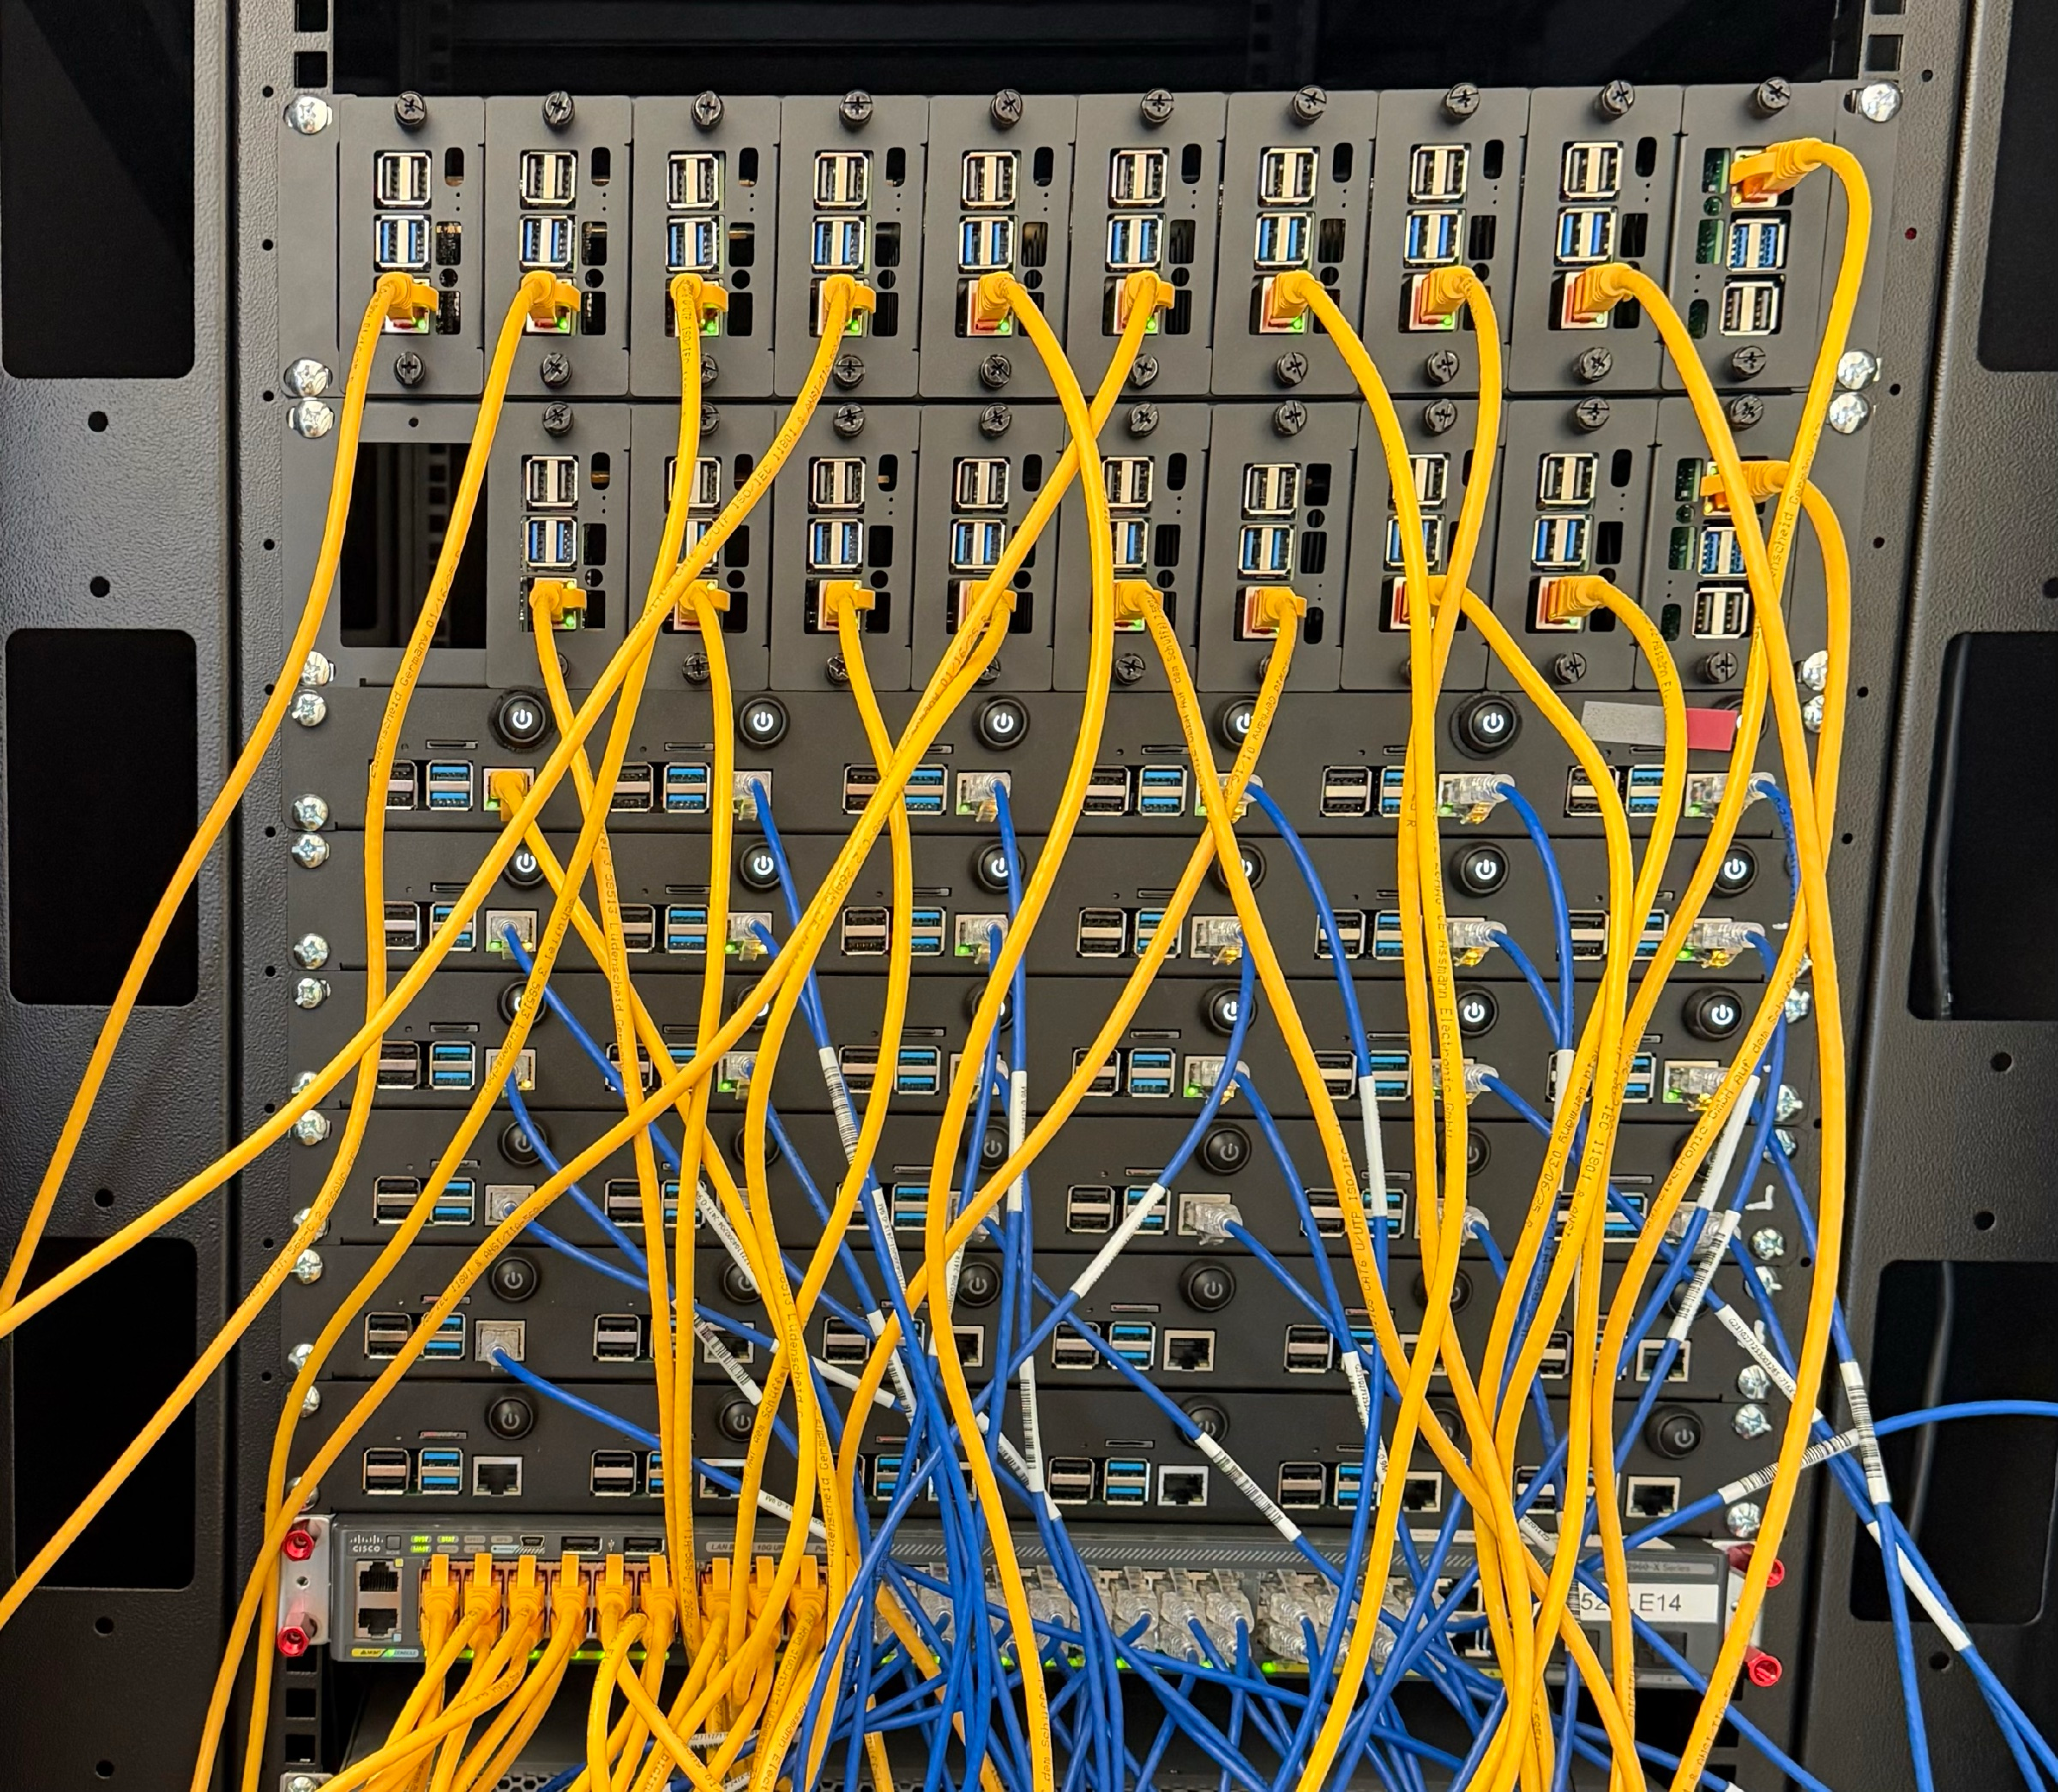
\includegraphics[width=0.72\textwidth]{figures/clusterpicture.pdf}
\caption{\textbf{Physical Raspberry Pi worker pool used for the experiments.} The cluster provides the mixed \texttt{rpi4}/\texttt{rpi5} substrate used by \texttt{fedctl}; individual experiments select logical deployment slices from this shared hardware.}
\label{fig:cluster_physical_worker_pool}
\end{figure}

\section{Observability and Reproducibility}
\label{appendix:observability_reproducibility}

The observability layer is organised around the questions that the evaluation and operator need to answer.

\paragraph{Did the run finish, and with which config/image?}
The submit service records submission identity, runner arguments, reconstructed command, status, errors, and result location. W\&B records method, task, profile tag, submission ID, and attempt metadata. Together these fields provide operational and scientific provenance.

\paragraph{Which physical devices participated?}
Nomad placement metadata and client-app environment variables are propagated into client logs and metrics. The research app records device type, node identity where available, partition ID, model rate, and typed-partition metadata.

\paragraph{How long did local training and evaluation take?}
Client replies include training duration, evaluation duration, examples per second, number of examples, and model rate. These metrics support the compute timing diagnostics in Table~\ref{tab:compute_main_runtime} and Figure~\ref{fig:compute_cifar10_client_train_time}.

\paragraph{Did asynchronous methods underrepresent \texttt{rpi4} clients?}
The asynchronous loop logs accepted updates with device type, staleness, queue latency, training duration, client trip, server step, and applied weight. These outputs support the participation, staleness, and weight-share analyses in Figures~\ref{fig:network_async_participation_staleness}--\ref{fig:network_async_weight_violin}.

\paragraph{Which artefacts regenerate the tables and figures?}
W\&B histories and summaries provide curves, final scores, runtime, target status, and fairness summaries. Structured artefacts provide event-level and per-client rows; submit-service log archives provide operational evidence for debugging and repeatable execution.

\section{Submit-Service Web Interface}
\label{appendix:submit_service_web_interface}

The deployed submit-service UI is available at \href{http://fedctl.cl.cam.ac.uk}{\texttt{fedctl.cl.cam.ac.uk}}. It is the browser companion to the \texttt{fedctl submit} command group, not a separate control path. The CLI creates, streams, and retrieves runs; the UI keeps submissions visible after the launching terminal has closed.

The UI preserves status, queue position, blocked reason, failure message, reconstructed \texttt{fedctl submit run} request, deployment inputs, Nomad jobs, live or archived logs, and result artefacts. These fields make the web record a durable inspection surface rather than only a status dashboard.

Failed and completed runs therefore remain inspectable and reproducible. Completed records link metric artefacts back to the command, deploy config, image, runtime metadata, and role logs; failed records retain enough context to distinguish application errors, queue-capacity problems, placement failures, and runtime crashes.

The node inventory page exposes the dispatcher's capacity model: typed capacity across roles and device classes, including \texttt{rpi4} and \texttt{rpi5}, plus the resource class blocking a waiting run.

The screenshots below show representative run-detail views: terminal state and artefacts, reconstructed request, Nomad role mapping, and role logs.

\begin{figure}[H]
\centering
\begin{subfigure}[t]{0.48\textwidth}
\vspace{0pt}
\centering
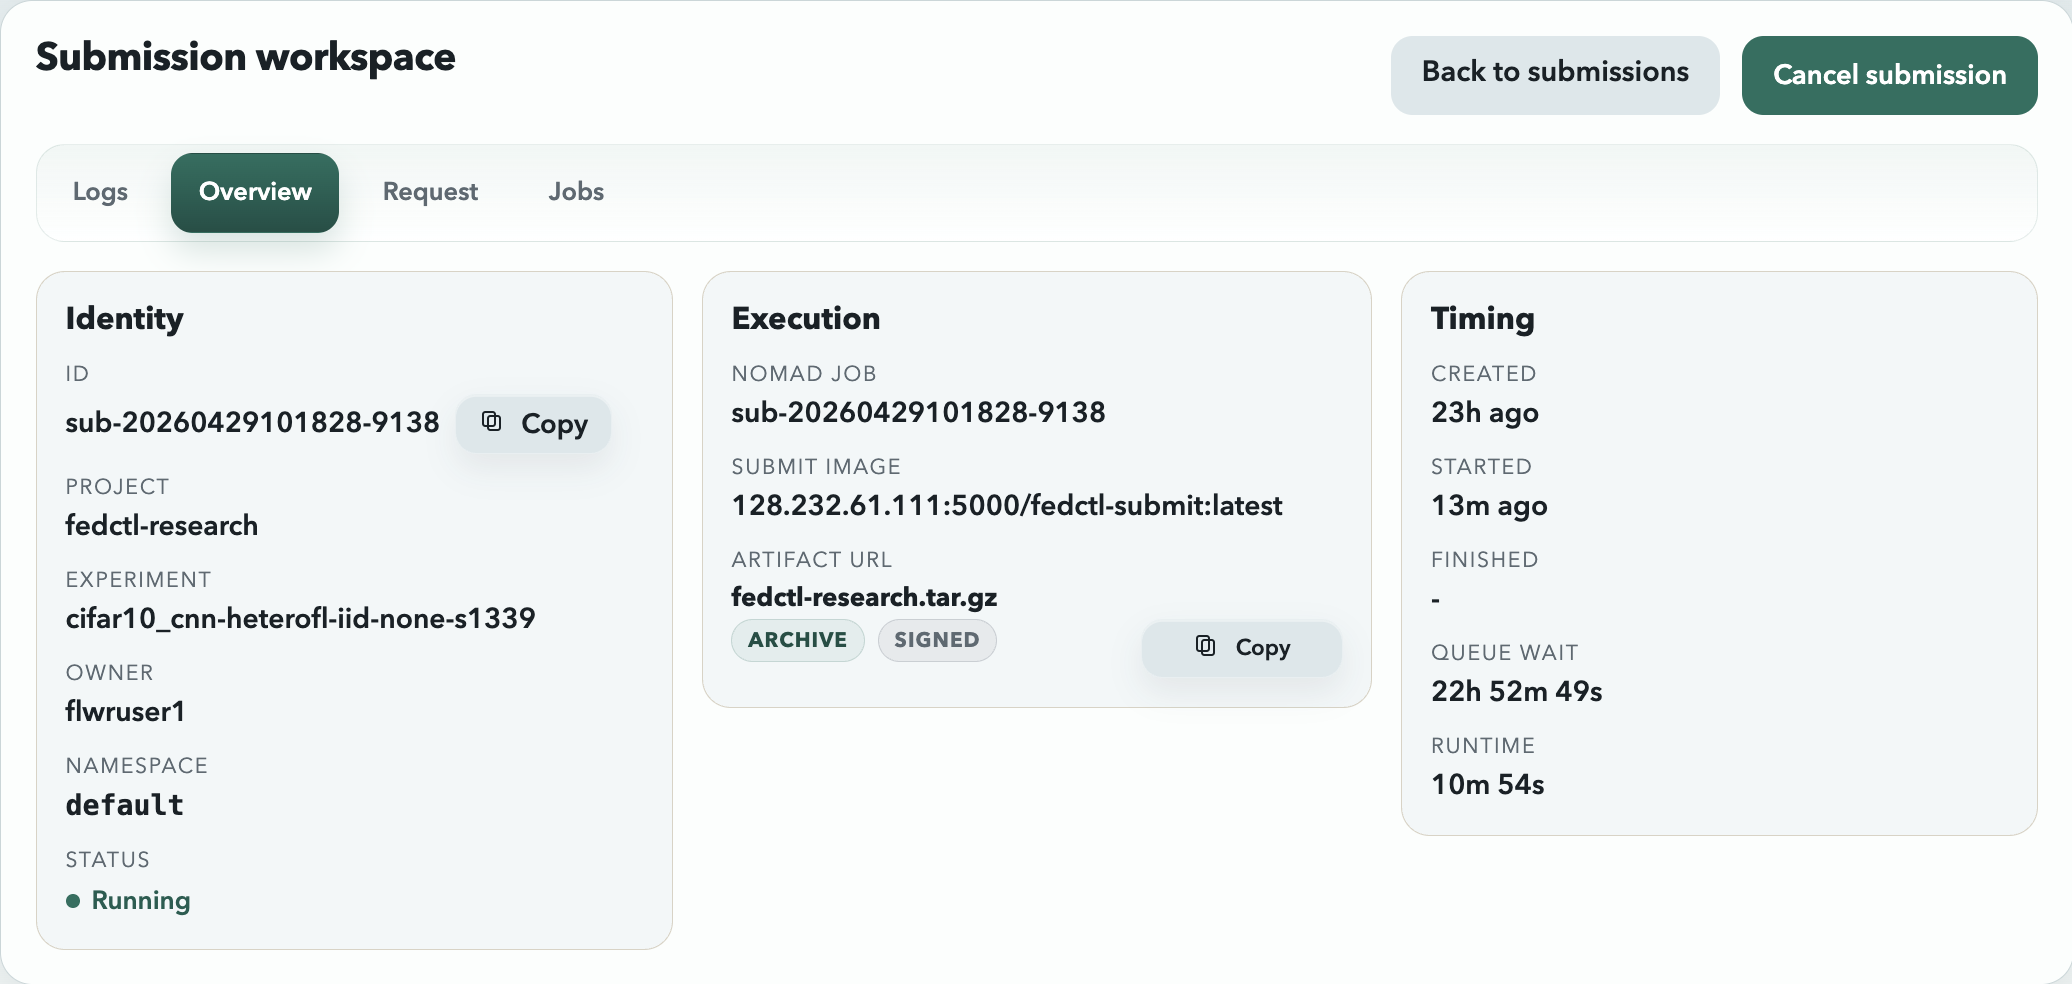
\includegraphics[width=\linewidth]{figures/detail_overview.png}
\caption{Run state and artefacts.}
\label{fig:submit_service_overview}
\end{subfigure}
\hfill
\begin{subfigure}[t]{0.48\textwidth}
\vspace{0pt}
\centering
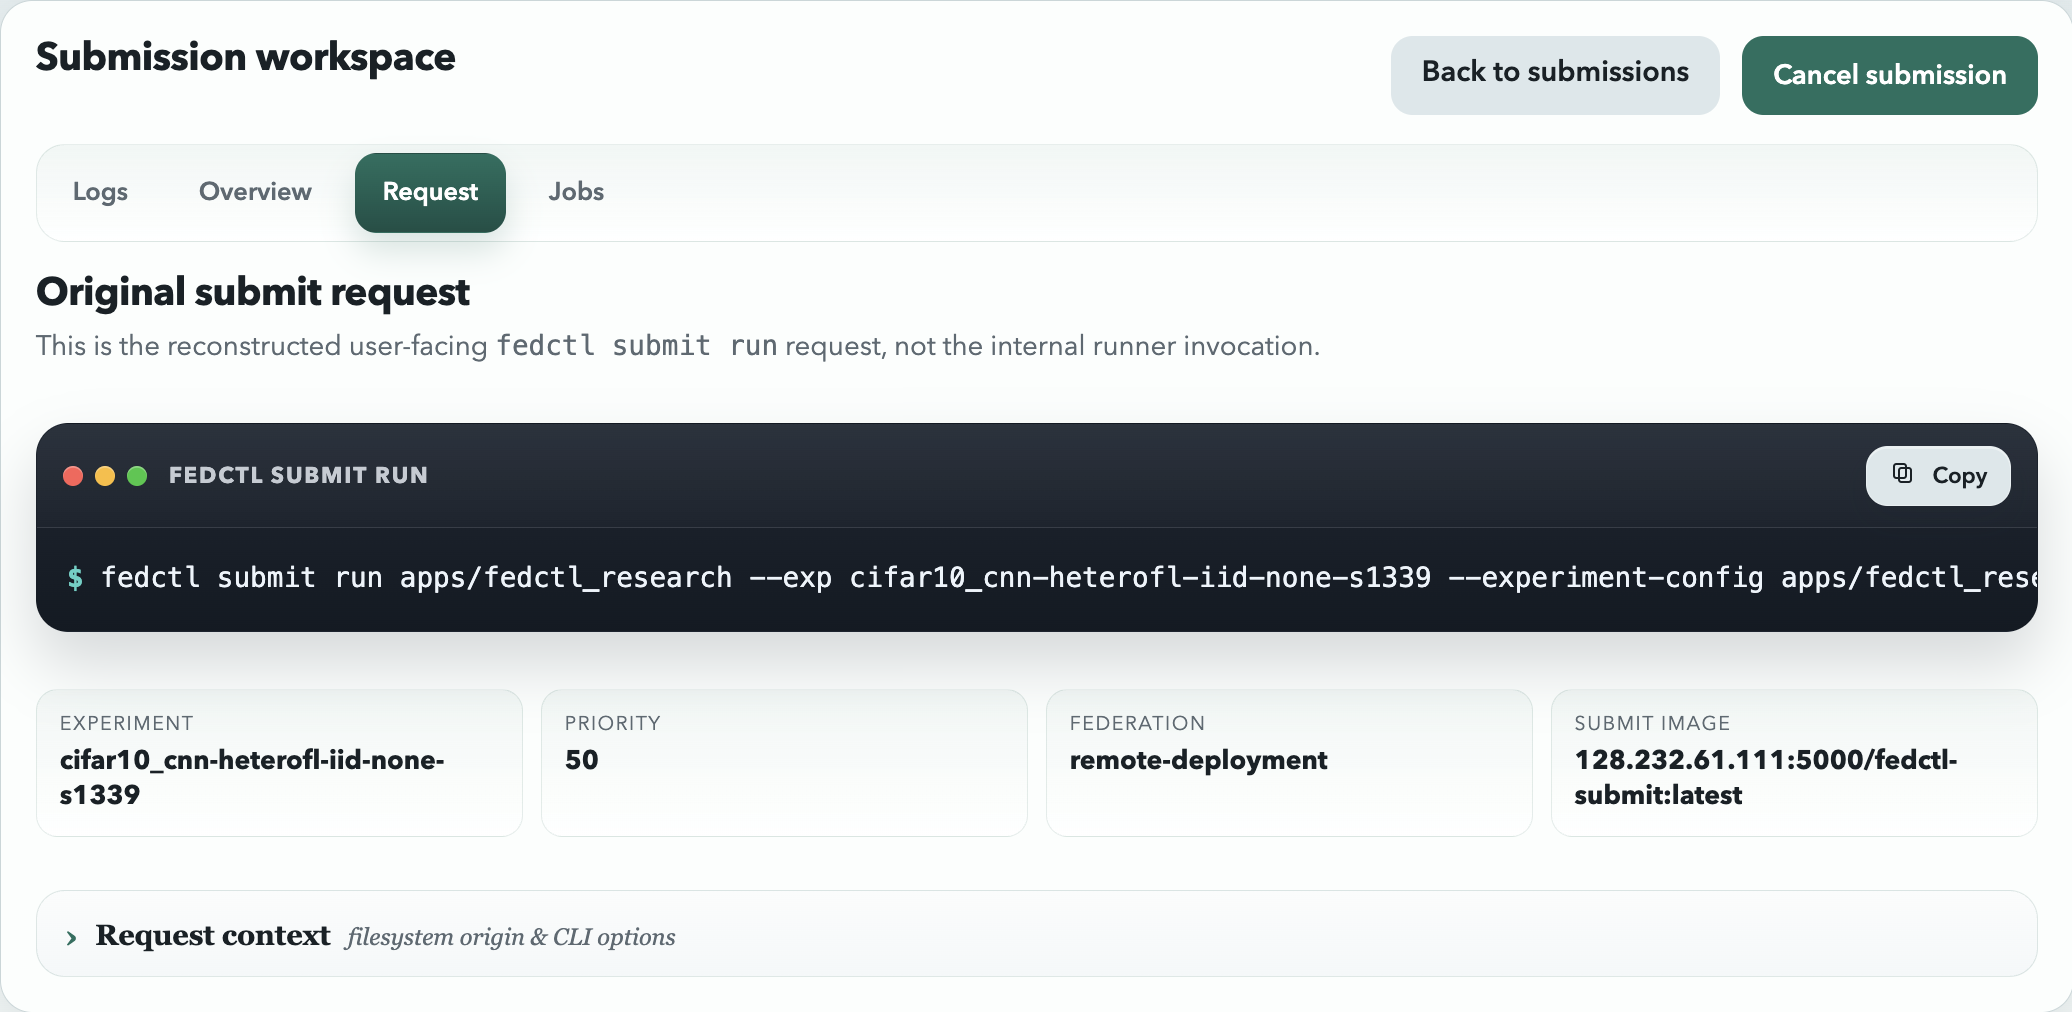
\includegraphics[width=\linewidth]{figures/detail_request.png}
\caption{Reconstructed request.}
\label{fig:submit_service_request}
\end{subfigure}
\par\vspace{0.6em}
\begin{subfigure}[t]{0.48\textwidth}
\vspace{0pt}
\centering
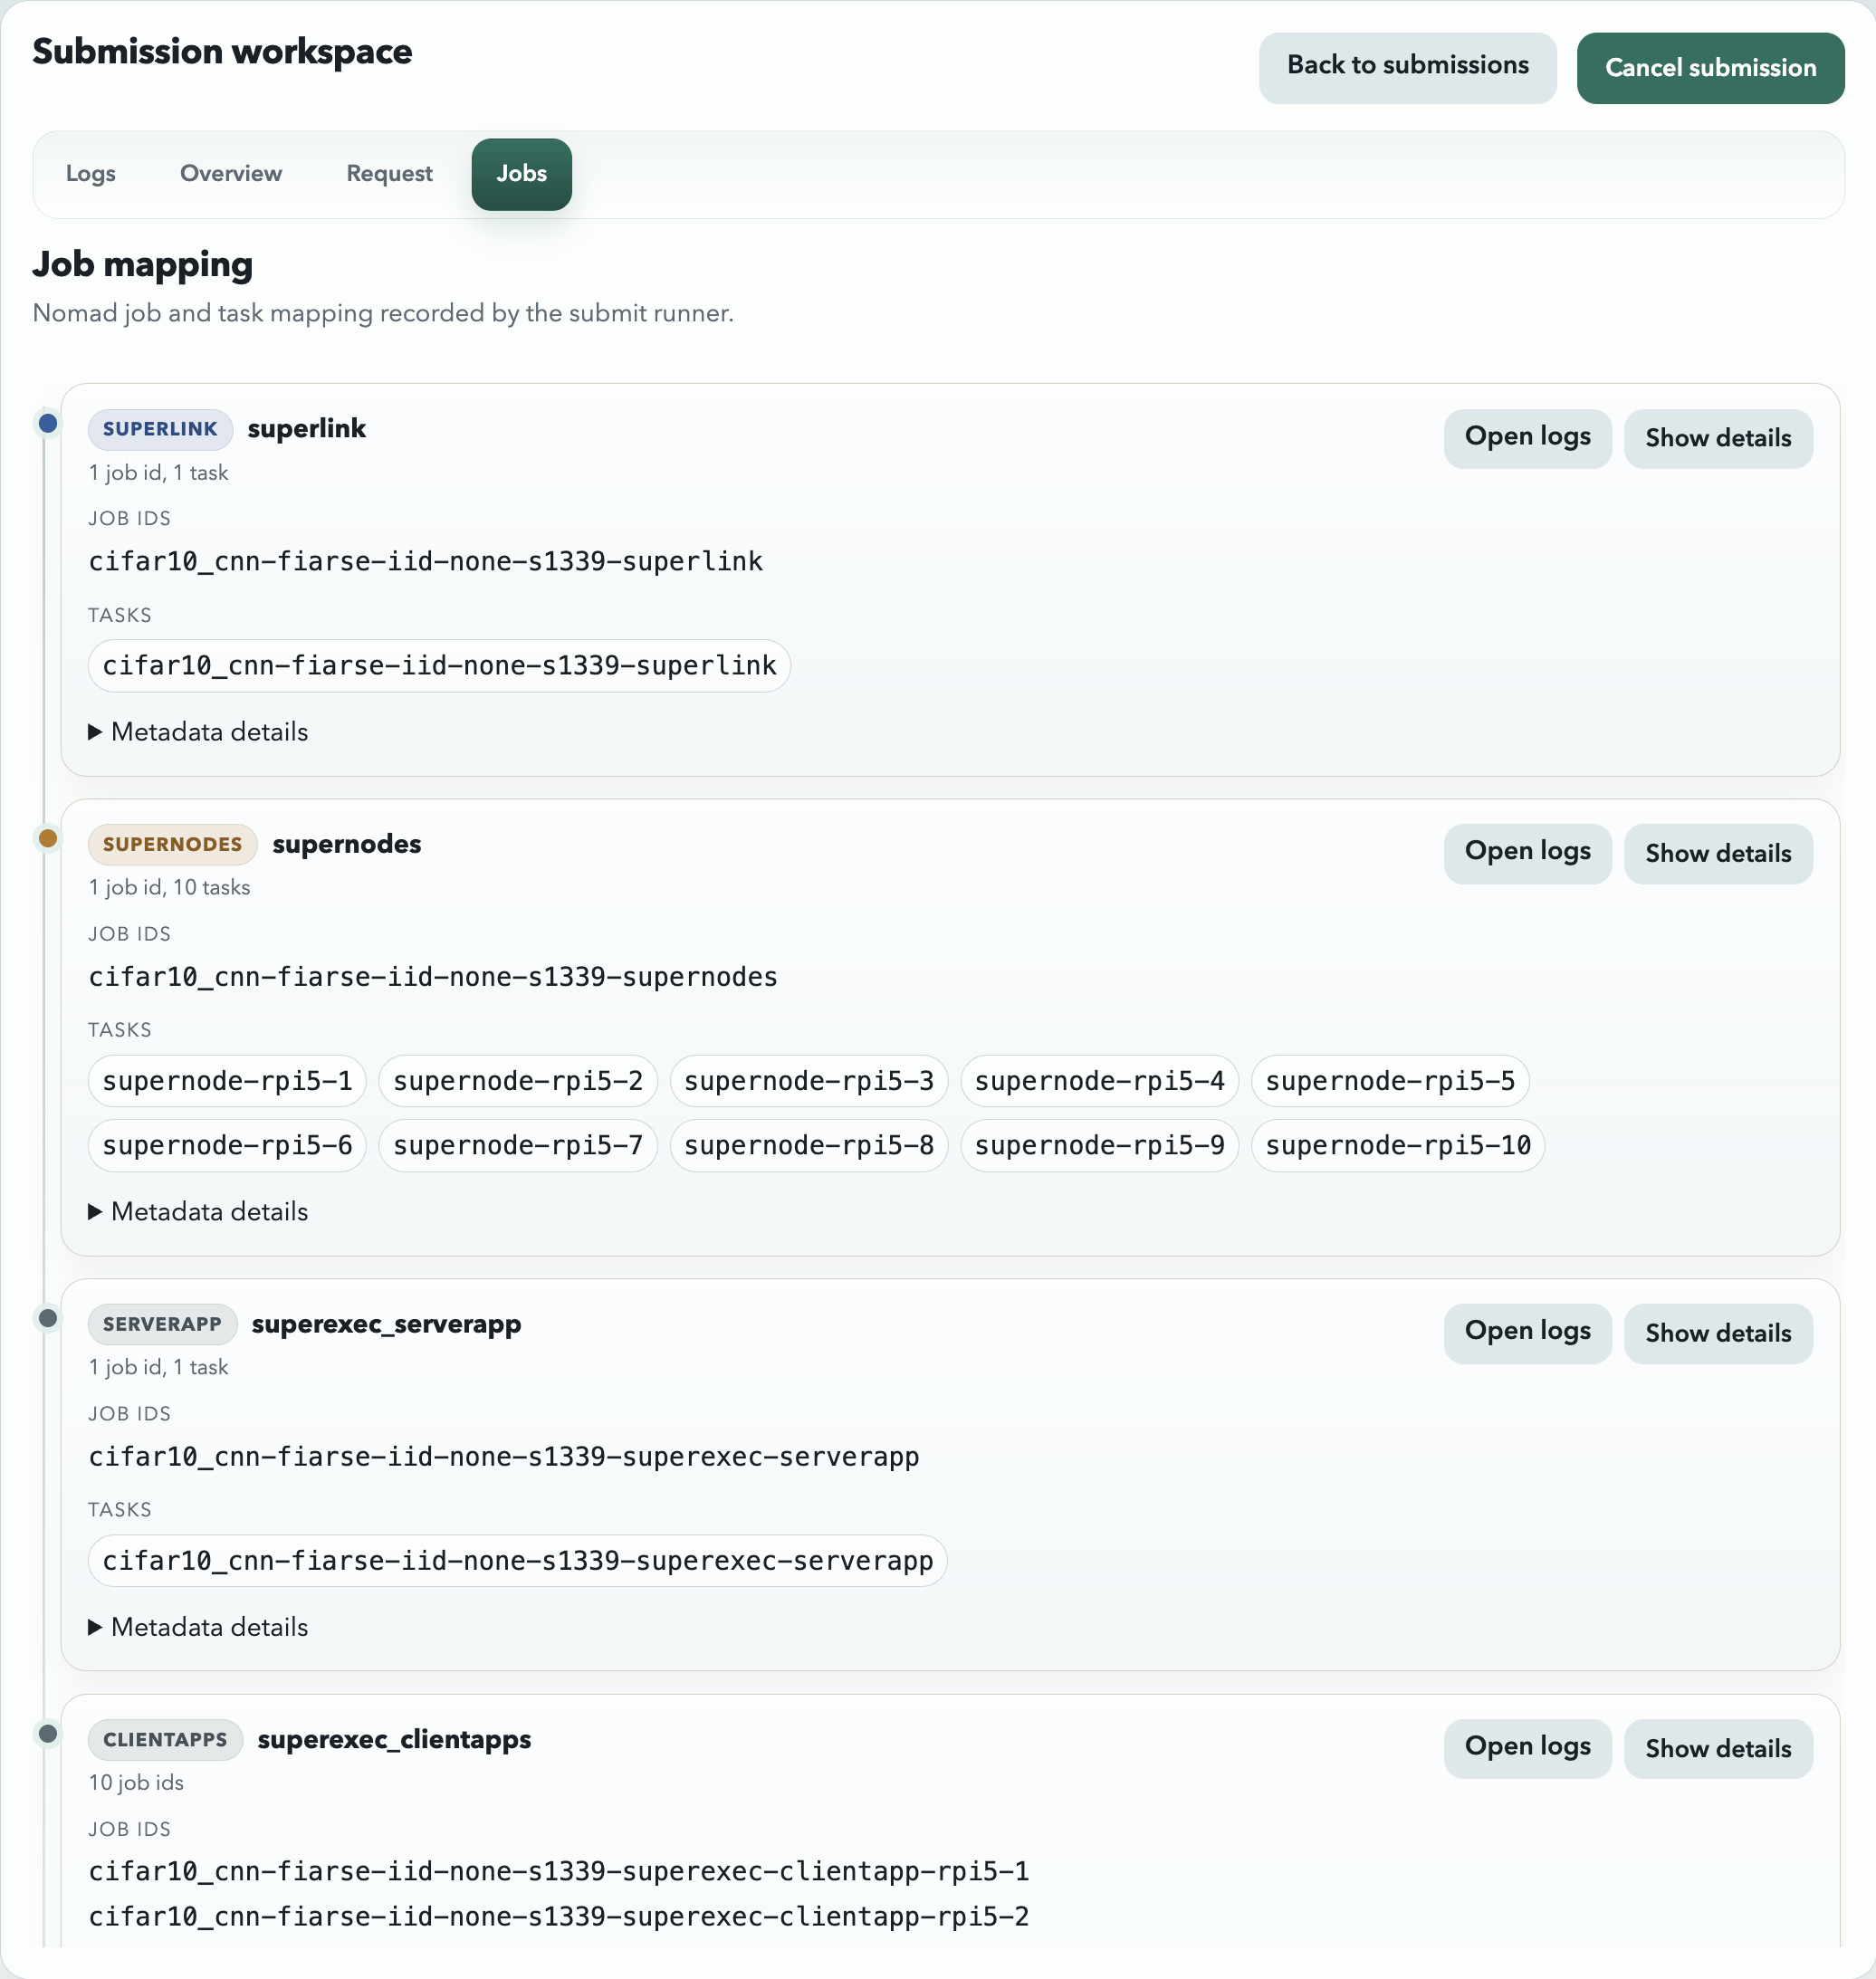
\includegraphics[width=\linewidth]{figures/detail_jobs.png}
\caption{Nomad role mapping.}
\label{fig:submit_service_jobs}
\end{subfigure}
\hfill
\begin{subfigure}[t]{0.48\textwidth}
\vspace{0pt}
\centering
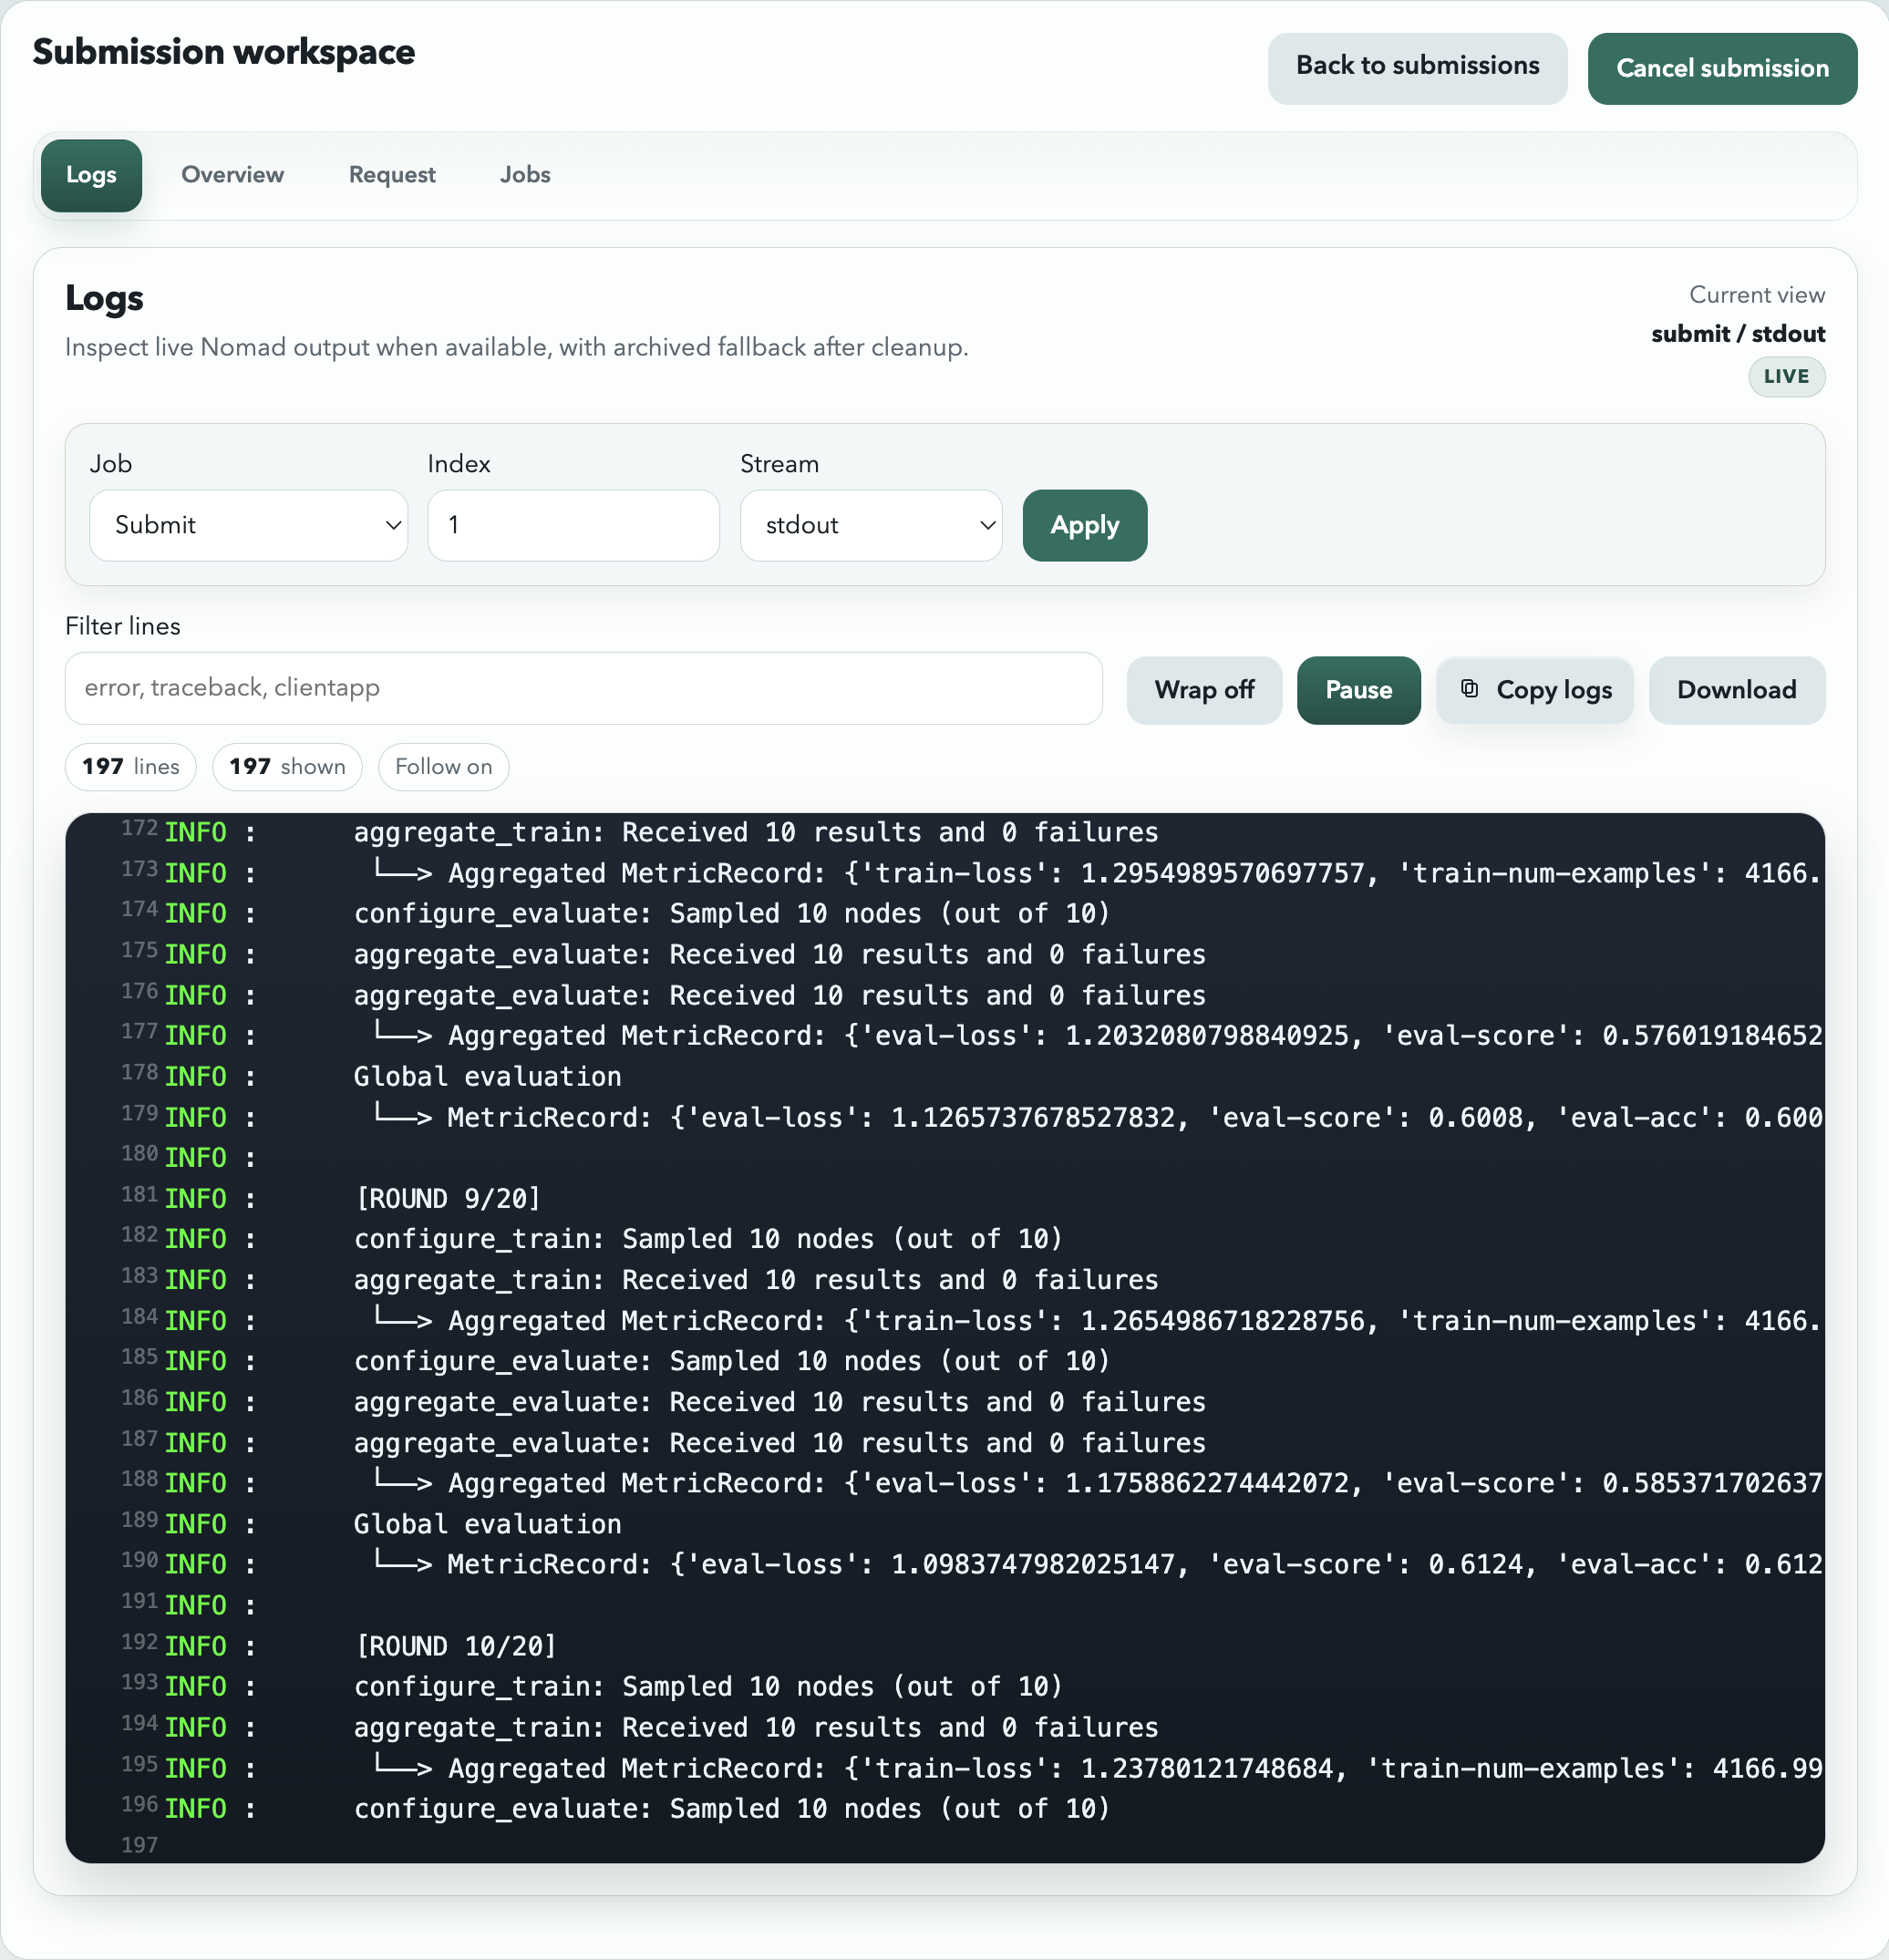
\includegraphics[width=\linewidth]{figures/detail_log.png}
\caption{Role logs.}
\label{fig:submit_service_logs}
\end{subfigure}
\caption{\textbf{Submit-service run-detail workspace.} The browser view keeps the state needed to reproduce, inspect, and debug a submitted run.}
\label{fig:submit_service_run_detail}
\end{figure}

% !TeX root = main.tex
\chapter{Evaluation Datasets}
\label{appendix:evaluation_tasks}

This appendix summarises the datasets and task models used in Chapter~\ref{chap:evaluation}. The purpose is to make the experimental workload clear without moving task-specific detail into the main systems and method narrative.

\section{Overview}

The evaluation uses three tasks. California Housing provides a lightweight tabular regression control, Fashion-MNIST provides a small image-classification workload, and CIFAR-10 provides the main compute-bound image-classification workload. All three are instantiated through the shared research-app task interface described in Chapter~\ref{chap:implementation}; the run configs then choose the partitioner, method, model-rate assignment, training budget, and deployment.

\section{California Housing Regression}
\label{appendix:california_housing_task}

\paragraph{Dataset.}
California Housing is a tabular regression dataset derived from California census block-group records \parencite{pace1997sparse}. Each example contains eight continuous attributes describing location, occupancy, rooms, population, and income. The prediction target is median house value. The dissertation uses the TensorFlow/Keras cached array with \(20{,}640\) examples, split into \(80\%\) training and \(20\%\) test data with a fixed seed. Features and targets are standardised using training-set statistics before model training.

\begin{figure}[H]
\centering
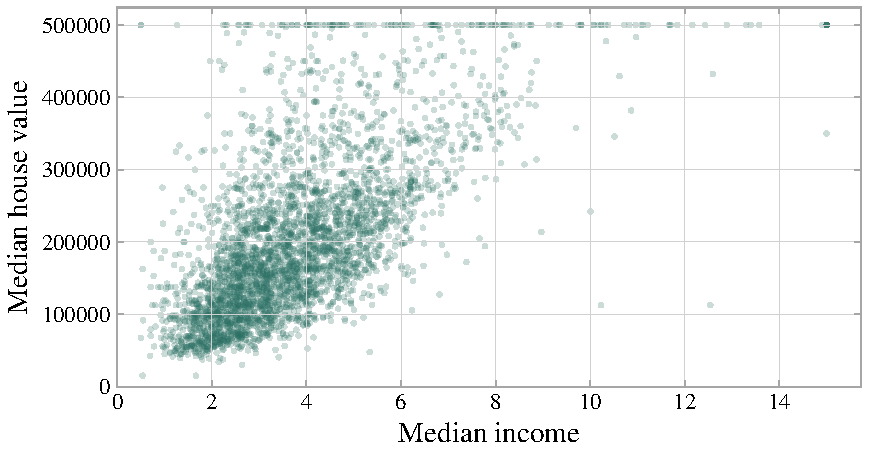
\includegraphics[width=0.56\textwidth]{figures/evaluation_task_california_housing_scatter.pdf}
\caption{\textbf{California Housing target relationship.} The scatter shows a deterministic sample of examples by median income and median house value before standardisation.}
\label{fig:appendix_california_housing_scatter}
\end{figure}

\paragraph{Model and partitioning.}
The task uses a width-scaled MLP with two hidden layers. At full rate, the hidden widths are \(128\) and \(64\); lower model rates reduce those widths while preserving the same input and output structure. IID runs split examples uniformly across clients. Non-IID runs use the continuous partitioner over a configured continuous feature, producing ordered partitions rather than label-skewed classification partitions.

\section{Fashion-MNIST Classification}
\label{appendix:fashion_mnist_task}

\paragraph{Dataset.}
Fashion-MNIST is a \(10\)-class image-classification dataset of clothing and accessory images \parencite{xiao2017fashionmnist}. Each example is a \(28\times28\) greyscale image. The dataset contains \(60{,}000\) training examples and \(10{,}000\) test examples. The implementation converts images to tensors and normalises them with mean \(0.2860\) and standard deviation \(0.3530\).

\begin{figure}[H]
\centering
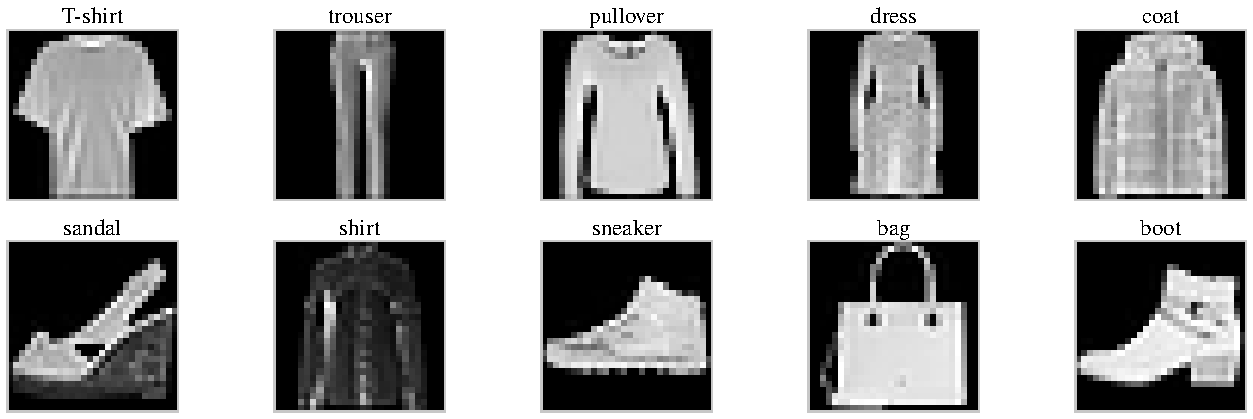
\includegraphics[width=0.64\textwidth]{figures/evaluation_task_fashion_mnist_samples.pdf}
\caption{\textbf{Sample Fashion-MNIST images.} One example is shown for each class.}
\label{fig:appendix_fashion_mnist_samples}
\end{figure}

\paragraph{Model and partitioning.}
The task uses a compact width-scaled CNN with two convolutional blocks and a linear classifier. At full rate, the convolutional widths are \(32\) and \(64\); lower model rates reduce the channel counts. IID runs split examples uniformly across clients. Non-IID runs use Dirichlet label-skew partitioning with \(\alpha=0.3\), matching the CIFAR-10 image-classification regime used for the main method comparisons.

\section{CIFAR-10 Classification}
\label{appendix:cifar10_task}

\paragraph{Dataset.}
CIFAR-10 is a standard \(10\)-class natural-image classification dataset \parencite{krizhevsky2009cifar}. Each example is a \(32\times32\) RGB image, and the dataset contains \(50{,}000\) training examples and \(10{,}000\) test examples. The implementation converts images to tensors and normalises channels with mean \((0.4914,0.4822,0.4465)\) and standard deviation \((0.2470,0.2435,0.2616)\).

\begin{figure}[H]
\centering
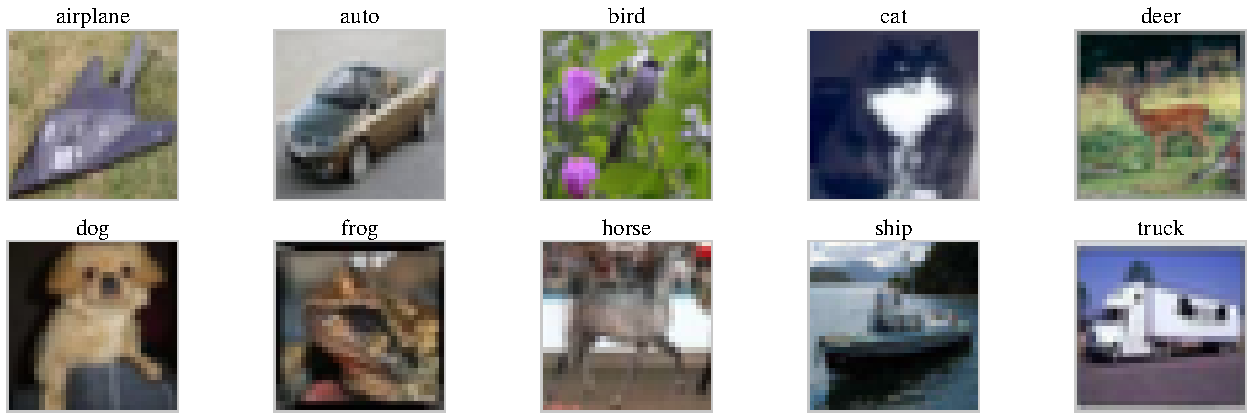
\includegraphics[width=0.64\textwidth]{figures/evaluation_task_cifar10_samples.pdf}
\caption{\textbf{Sample CIFAR-10 images.} One example is shown for each class.}
\label{fig:appendix_cifar10_samples}
\end{figure}

\paragraph{Model and partitioning.}
The task uses a width-scaled CNN with three convolutional blocks, adaptive average pooling, and a linear classifier. At full rate, the convolutional widths are \(64\), \(128\), and \(256\). This makes CIFAR-10 the most compute-bound workload in the evaluation and the clearest test of whether submodel FL reduces local training cost. IID runs split examples uniformly across clients, while non-IID runs use Dirichlet label-skew partitioning with \(\alpha=0.3\).

% !TeX root = main.tex
\chapter{Reproducibility Material}
\label{appendix:reproducibility_material}

This appendix records the current configuration families used to reproduce the dissertation experiments. It is intentionally limited to the active run and deployment surfaces: the older exploratory branches remain in the repository, but are not part of the main evaluation story in Chapter~\ref{chap:evaluation}.

\section{Evaluation Settings}
\label{appendix:evaluation_settings}

The tables below collect the main run settings that are referenced but not repeated in Chapter~\ref{chap:evaluation}. They are summaries of the resolved run and deploy configs, not a replacement for the archived artefacts attached to each submitted run.

\begin{table}[!htbp]
\centering
\caption{Main compute-heterogeneity benchmark settings.}
\label{tab:appendix_compute_settings}
\footnotesize
\begin{tabularx}{\textwidth}{>{\raggedright\arraybackslash}p{0.28\textwidth}X}
\toprule
Setting & Value \\
\midrule
Deployment & \(20\) logical clients on \(10\times\texttt{rpi4}+10\times\texttt{rpi5}\). \\
Tasks & \texttt{california\_housing\_mlp}, \texttt{fashion\_mnist\_cnn}, and \texttt{cifar10\_cnn}. \\
Methods & \texttt{FedAvg}, \texttt{HeteroFL}, \texttt{FedRolex}, and \texttt{FIARSE}. \\
Model-rate assignment & \(0.125,0.25\) on \texttt{rpi4}; \(0.5,1.0\) on \texttt{rpi5}; \(5\) clients per rate group. \\
Batch sizes & CIFAR-10 and Fashion-MNIST: \texttt{rpi4}=8, \texttt{rpi5}=32. California Housing: \texttt{rpi4}=32, \texttt{rpi5}=128. \\
Data regimes & IID with matched dataset caps; CIFAR-10 and Fashion-MNIST non-IID Dirichlet \(\alpha=0.3\); California Housing non-IID continuous-feature split. \\
Optimisation and metrics & Classification reports accuracy; regression uses \texttt{Adam} and reports \(R^2\). \\
Seeds & \(1337\)--\(1339\), unless a figure caption states a diagnostic rerun seed. \\
\bottomrule
\end{tabularx}
\end{table}

\begin{table}[!htbp]
\centering
\caption{Main straggler-induced heterogeneity benchmark settings.}
\label{tab:appendix_straggler_settings}
\footnotesize
\begin{tabularx}{\textwidth}{>{\raggedright\arraybackslash}p{0.28\textwidth}X}
\toprule
Setting & Value \\
\midrule
Task & \texttt{cifar10\_cnn}. \\
Design & \(2\times2\) matrix over data regime (IID/non-IID) and topology (all-\texttt{rpi5}/mixed). \\
Deployments & \(15\) logical clients. The homogeneous control uses \(15\times\texttt{rpi5}\); the mixed treatment uses \(10\times\texttt{rpi5}+5\times\texttt{rpi4}\). \\
Methods & \texttt{FedAvg}, \texttt{FedAsync}, \texttt{FedBuff}, and \texttt{FedStaleWeight}; compact tables abbreviate \texttt{FedStaleWeight} as \texttt{FedSW}. \\
Budgets & \texttt{FedAvg}: \(50\) rounds. Asynchronous methods: \(100\) server steps and \texttt{train-concurrency}=15. \\
Buffered settings & Main \texttt{FedBuff}/\texttt{FedStaleWeight} runs use \(K=10\); the network-stressor sweep also includes \(K=5\) variants. \\
Endpoint & First validation accuracy \(\ge 60\%\), reported by completed client trips and wall-clock time. \\
Seeds & \(1337\)--\(1339\). \\
\bottomrule
\end{tabularx}
\end{table}

\begin{table}[!htbp]
\centering
\caption{Asynchronous-submodel and \texttt{FedCover} benchmark settings.}
\label{tab:appendix_fedcover_settings}
\footnotesize
\begin{tabularx}{\textwidth}{>{\raggedright\arraybackslash}p{0.28\textwidth}X}
\toprule
Setting & Value \\
\midrule
Deployment & \(20\) logical clients on \(10\times\texttt{rpi4}+10\times\texttt{rpi5}\). \\
Tasks and data & CIFAR-10 and Fashion-MNIST under IID and Dirichlet non-IID \(\alpha=0.3\). \\
Submodel assignment & Nested \texttt{HeteroFL} rates \(0.125,0.25,0.5,1.0\), matched to the compute-heterogeneity assignment. \\
Methods & Synchronous \texttt{HeteroFL}, uncorrected \texttt{Async-HeteroFL}, \texttt{FedCover} with \(\gamma\in\{0.25,0.5,1.0,1.5\}\), and \texttt{FedBuff}. \\
Targets & CIFAR-10: \(70\%\) IID and \(60\%\) non-IID. Fashion-MNIST: \(80\%\) IID and \(75\%\) non-IID. \\
Warm-up adjustment & Post-warm-up time subtracts the first \(20\) completed client trips: one synchronous \texttt{HeteroFL} round or five \(K=4\) asynchronous buffer updates. \\
Seeds & \(1337\)--\(1339\). \\
\bottomrule
\end{tabularx}
\end{table}

\FloatBarrier
\section{Run-Config Families}

Application-side choices are stored under \path{apps/fedctl_research/run_configs/}. These TOML files use the sectioned run-config schema described in Chapter~\ref{chap:implementation}; \texttt{fedctl} lowers the sectioned form into the flat Flower run config passed to the application.

\begin{table}[!htbp]
\centering
\caption{Active run-config families for the dissertation evaluation.}
\label{tab:appendix_run_config_families}
\footnotesize
\begin{tabularx}{\textwidth}{>{\raggedright\arraybackslash}p{0.41\textwidth}X}
\toprule
Run-config family & Role in the evaluation \\
\midrule
\path{compute_heterogeneity/main/cifar10_cnn/} & Main compute-heterogeneity classification evaluation under IID and non-IID splits. \\
\path{compute_heterogeneity/main/california_housing_mlp/} & Main compute-heterogeneity tabular-regression evaluation under IID and non-IID splits. \\
\path{compute_heterogeneity/ablations/slow_minority/} & Slow-minority ablation comparing exclusion, full-model inclusion, and reduced-rate inclusion of slower devices. \\
\path{compute_heterogeneity/ablations/slow_majority/} & Slow-majority rerun family for the updated weak-client inclusion decision. \\
\path{network_heterogeneity/main/cifar10_cnn/} & Main asynchronous target-attainment matrix over IID/non-IID data and mixed/all-\texttt{rpi5} topologies. \\
\path{network_heterogeneity/ablations/network_stressor_sweep/cifar10_cnn/} & Network-stressor sweep used to separate straggler effects from artificial link impairment. \\
\path{network_heterogeneity/ablations/device_correlated_non_iid/cifar10_cnn/} & Device-correlated non-IID experiment where slower devices hold systematically different classes. \\
\path{compute_heterogeneity/ablations/fedcover_pilot/} & Asynchronous-submodel and \texttt{FedCover} evaluation under CIFAR-10 and Fashion-MNIST. \\
\bottomrule
\end{tabularx}
\end{table}

\FloatBarrier
\section{Deployment Presets}

Deploy config choices are stored under \path{apps/fedctl_research/deploy_configs/}. These YAML files fix the physical or logical device pool, placement policy, resource reservations, submit-service endpoint, and optional \texttt{netem} profiles. The main presets used by the evaluation are summarised in Table~\ref{tab:appendix_deploy_presets}.

\begin{table}[!htbp]
\centering
\caption{Representative deploy config presets used by the evaluation.}
\label{tab:appendix_deploy_presets}
\footnotesize
\begin{tabularx}{\textwidth}{>{\raggedright\arraybackslash}p{0.42\textwidth}>{\centering\arraybackslash}p{0.16\textwidth}X}
\toprule
Deployment preset & SuperNodes & Use \\
\midrule
\path{compute_heterogeneity/main/none.yaml} & \(10\) \texttt{rpi4} + \(10\) \texttt{rpi5} & Main compute-heterogeneity runs on the mixed Raspberry Pi testbed. \\
\path{compute_heterogeneity/ablations/slow_minority/mixed.yaml} & \(3\) \texttt{rpi4} + \(12\) \texttt{rpi5} & Slow-minority inclusion experiment. \\
\path{compute_heterogeneity/ablations/slow_minority/rpi5_only.yaml} & \(12\) \texttt{rpi5} & Slow-minority exclusion control. \\
\path{network_heterogeneity/main/mixed/none.yaml} & \(5\) \texttt{rpi4} + \(10\) \texttt{rpi5} & Mixed-topology no-impairment asynchronous target-attainment runs. \\
\path{network_heterogeneity/main/all_rpi5/none.yaml} & \(15\) \texttt{rpi5} & Packed all-\texttt{rpi5} no-impairment control runs. \\
\path{network_heterogeneity/ablations/network_stressor_sweep/*.yaml} & \(5\) \texttt{rpi4} + \(10\) \texttt{rpi5} & Dedicated network-stressor sweep presets. \\
\path{network_heterogeneity/ablations/device_correlated_non_iid/none.yaml} & \(5\) \texttt{rpi4} + \(10\) \texttt{rpi5} & Device-correlated non-IID fairness experiment. \\
\bottomrule
\end{tabularx}
\end{table}

\FloatBarrier
\section{Network Profiles}

The network-stressor sweep uses named \texttt{netem} profiles from the dedicated network-stressor deploy config presets. The default dissertation deployment applies impairment at the SuperNode role; SuperExec wrappers can be enabled separately but are disabled in these presets.

\begin{table}[!htbp]
\centering
\caption{Network-stressor profiles used in the asynchronous sweep.}
\label{tab:appendix_network_profiles}
\footnotesize
\begin{tabularx}{\textwidth}{>{\raggedright\arraybackslash}p{0.16\textwidth}>{\centering\arraybackslash}p{0.13\textwidth}>{\centering\arraybackslash}p{0.13\textwidth}>{\centering\arraybackslash}p{0.13\textwidth}>{\centering\arraybackslash}p{0.13\textwidth}X}
\toprule
Profile & Delay & Jitter & Loss & Rate & Direction \\
\midrule
\texttt{none} & -- & -- & -- & -- & No artificial impairment. \\
\texttt{mild} & \(20\) ms & \(5\) ms & \(0.0\%\) & \(100\) Mbit/s & Symmetric. \\
\texttt{med} & \(60\) ms & \(15\) ms & \(0.5\%\) & \(50\) Mbit/s & Symmetric. \\
\texttt{asym\_up} & \(90\) ms & \(20\) ms & \(0.5\%\) & \(20\) Mbit/s & Egress impaired, ingress left as \texttt{none}. \\
\texttt{asym\_down} & \(90\) ms & \(20\) ms & \(0.5\%\) & \(20\) Mbit/s & Ingress impaired, egress left as \texttt{none}. \\
\bottomrule
\end{tabularx}
\end{table}

\FloatBarrier
\section{Representative Commands}

The following commands show the reproducibility pattern rather than every submitted run. Multi-seed runs are encoded by the run config itself, and a single run can be forced with \verb|--seed| when needed.

\begin{codeblock}[minted options app={breaklines,breakanywhere,fontsize=\footnotesize}]{bash}
fedctl submit run apps/fedctl_research \
  --run-config apps/fedctl_research/run_configs/compute_heterogeneity/main/cifar10_cnn/iid/fedrolex.toml \
  --deploy-config apps/fedctl_research/deploy_configs/compute_heterogeneity/main/none.yaml \
  --stream
\end{codeblock}

\begin{codeblock}[minted options app={breaklines,breakanywhere,fontsize=\footnotesize}]{bash}
fedctl submit run apps/fedctl_research \
  --run-config apps/fedctl_research/run_configs/network_heterogeneity/main/cifar10_cnn/noniid/mixed/fedasync.toml \
  --deploy-config apps/fedctl_research/deploy_configs/network_heterogeneity/main/mixed/none.yaml \
  --stream
\end{codeblock}

\begin{codeblock}[minted options app={breaklines,breakanywhere,fontsize=\footnotesize}]{bash}
fedctl submit run apps/fedctl_research \
  --run-config apps/fedctl_research/run_configs/network_heterogeneity/ablations/network_stressor_sweep/cifar10_cnn/fedstaleweight.toml \
  --deploy-config apps/fedctl_research/deploy_configs/network_heterogeneity/ablations/network_stressor_sweep/med.yaml \
  --stream
\end{codeblock}

For archival runs, the submit artefact stores the resolved request, copied external run config as \path{.fedctl/run_config.toml} when applicable, deployment metadata, role logs, and result artefacts. This is the reproducibility surface used by the submit-service UI and by the result retrieval workflow.

% !TeX root = main.tex
\chapter{Additional Figures}
\label{appendix:additional_figures}

This appendix collects supporting diagnostic figures that are useful for interpreting Chapter~\ref{chap:evaluation}, but too detailed for the main evaluation flow.

\section{FedAsync Accepted-Update Staleness}
\label{appendix:fedasync_staleness_heatmap}

Figure~\ref{fig:appendix_network_fedasync_participation_staleness} gives the \texttt{FedAsync}-only accepted-update trace corresponding to the buffered asynchronous diagnostics in Section~\ref{sec:eval_network_heterogeneity}. Because \texttt{FedAsync} applies one reply at a time, its server step is also a completed client trip.

\begin{figure}[H]
\centering
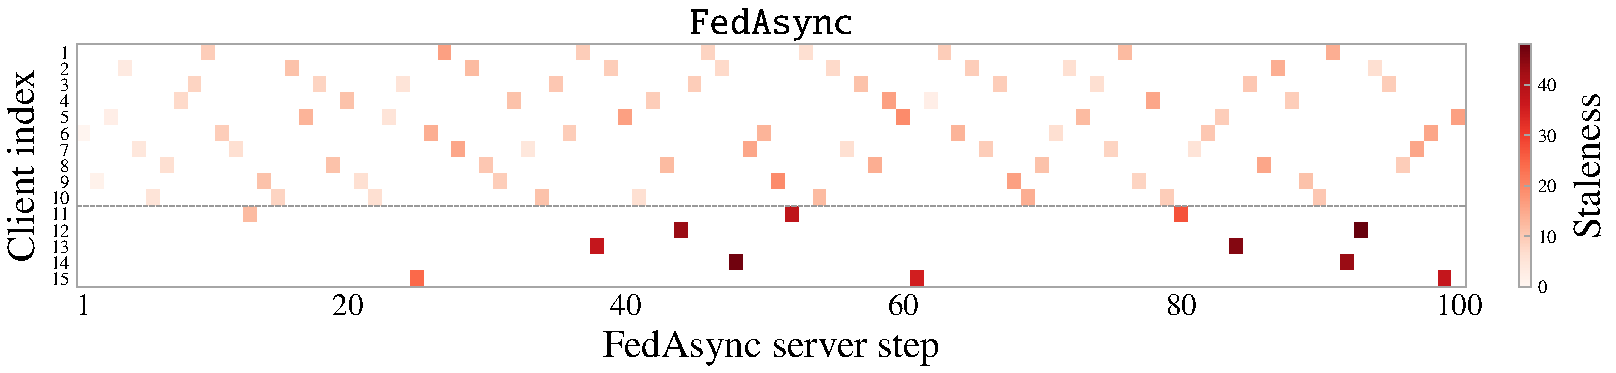
\includegraphics[width=\textwidth]{figures/network_fedasync_participation_staleness.pdf}
% Notes: rows 1--10 are rpi5 client slots; rows 11--15 are rpi4 client slots.
% White cells indicate no accepted update; darker blue indicates larger accepted-update staleness.
\caption{\textbf{\texttt{FedAsync} accepted client updates in mixed non-IID runs.} The heatmap shows the first \(100\) accepted updates on the mixed \texttt{rpi5}/\texttt{rpi4} topology, using the same device-slot convention as Figure~\ref{fig:network_async_participation_staleness}.}
\label{fig:appendix_network_fedasync_participation_staleness}
\end{figure}

\section{Fashion-MNIST Local Submodel Accuracy}
\label{appendix:fashion_mnist_local_submodel_dist}

Figure~\ref{fig:appendix_compute_fashion_mnist_local_submodel_grid} gives the Fashion-MNIST counterpart to the CIFAR-10 local-submodel diagnostic in Figure~\ref{fig:compute_cifar10_seed1340_local_submodel_grid}. It pools the per-client extracted-submodel evaluations from seeds \texttt{1337}, \texttt{1338}, and \texttt{1339}.

\begin{figure}[H]
\centering
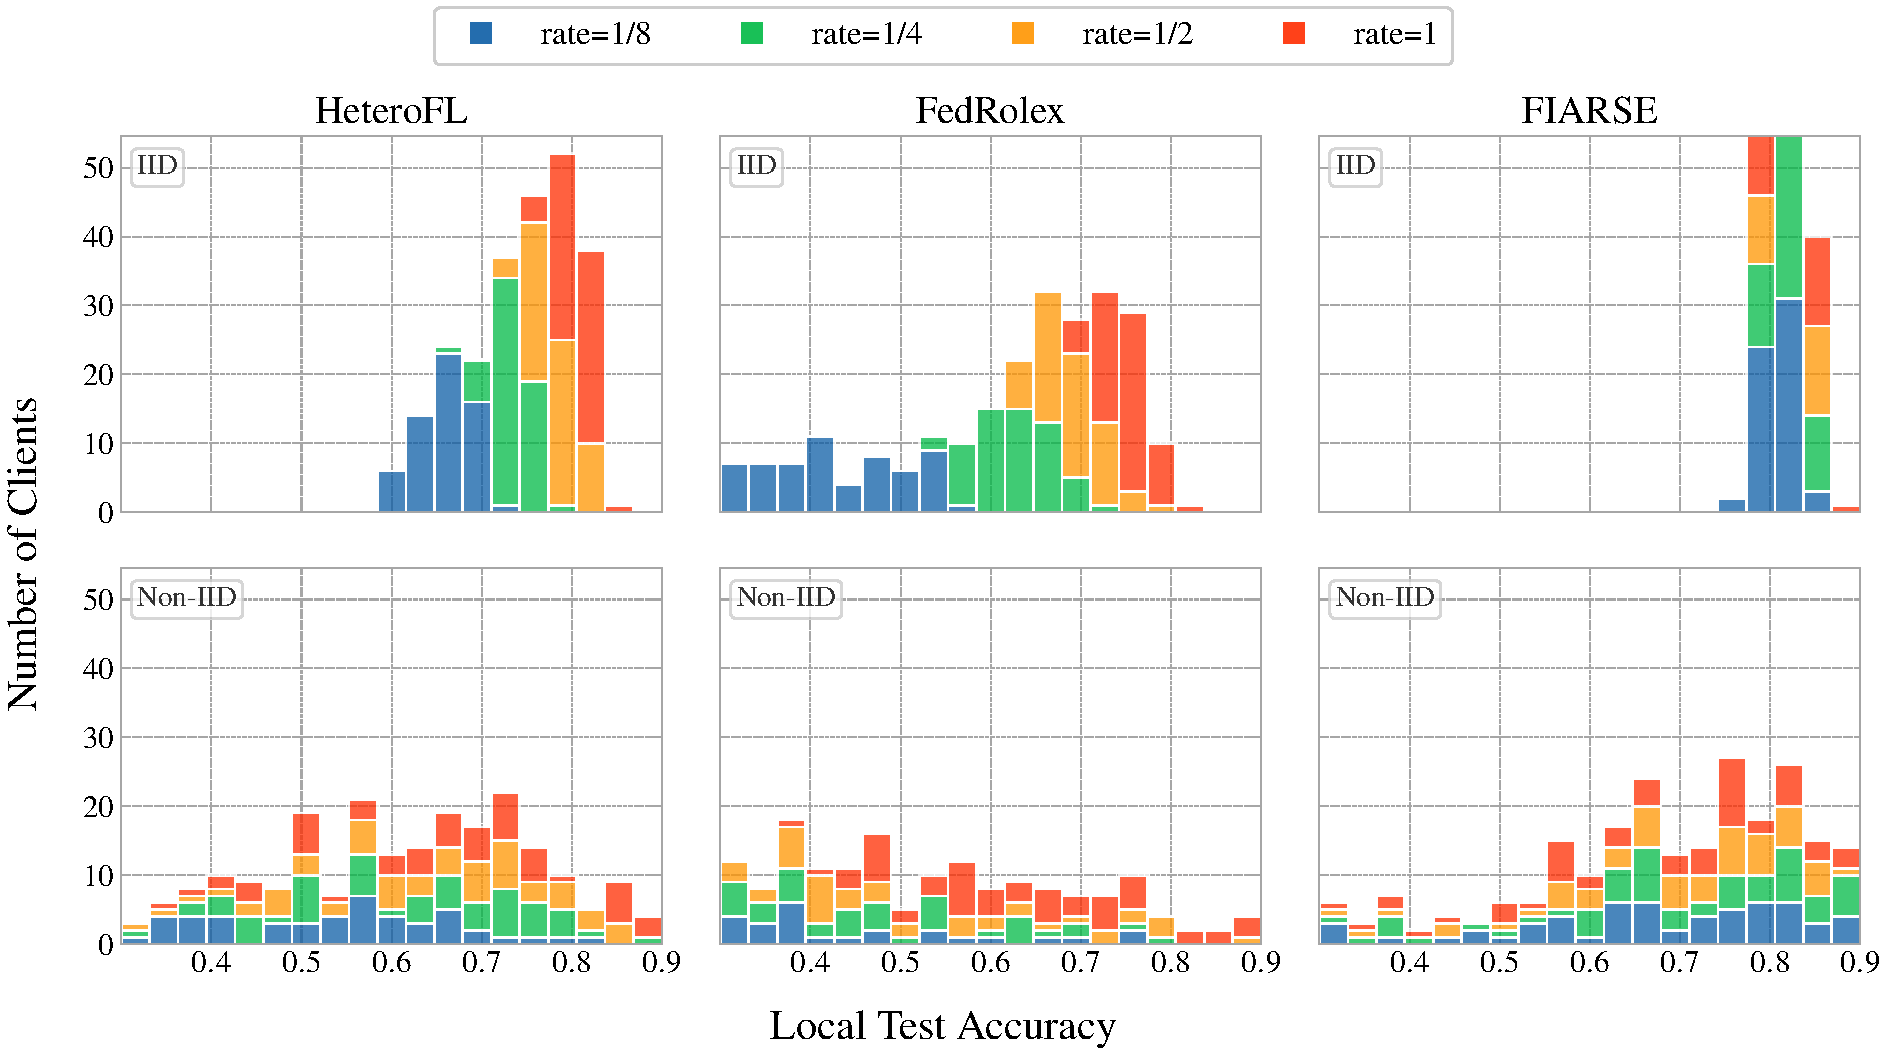
\includegraphics[width=0.98\textwidth]{figures/compute_main_fashion_mnist_local_submodel_grid.pdf}
% Notes: rows are IID/non-IID and columns are HeteroFL, FedRolex, and FIARSE.
% Each panel pools final local-submodel evaluations for rates 0.125, 0.25, 0.5, and 1.0 across seeds 1337, 1338, and 1339.
% Accuracy is measured on each client's local evaluation partition, not the global test set.
\caption{\textbf{Client-level Fashion-MNIST local submodel accuracy distributions.}}
\label{fig:appendix_compute_fashion_mnist_local_submodel_grid}
\end{figure}

\section{Fashion-MNIST Client Training Time}
\label{appendix:fashion_mnist_client_train_time}

Figure~\ref{fig:appendix_compute_fashion_mnist_client_train_time} gives the Fashion-MNIST counterpart to the CIFAR-10 timing diagnostic in Figure~\ref{fig:compute_cifar10_client_train_time}. It uses seed \texttt{1338} and the same device-rate grouping convention.

\begin{figure}[H]
\centering

\includegraphics[width=0.98\textwidth]{figures/compute_main_fashion_mnist_seed1338_client_train_time.pdf}
% Notes: rows are IID/non-IID and columns are HeteroFL, FedRolex, and FIARSE.
% Curves show mean update_train_duration_s for each device/rate group per server round.
% Shaded bands show within-group standard deviation across clients.
% IID runs contain 20 rounds; non-IID runs contain 40 rounds.
\caption{\textbf{Per-round client training time on Fashion-MNIST.}}
\label{fig:appendix_compute_fashion_mnist_client_train_time}
\end{figure}


\label{lastpage}
\end{document}
